\documentclass[twoside]{book}

% Packages required by doxygen
\usepackage{calc}
\usepackage{doxygen}
\usepackage{graphicx}
\usepackage[utf8]{inputenc}
\usepackage{makeidx}
\usepackage{multicol}
\usepackage{multirow}
\usepackage{textcomp}
\usepackage[table]{xcolor}

% Font selection
\usepackage[T1]{fontenc}
\usepackage{mathptmx}
\usepackage[scaled=.90]{helvet}
\usepackage{courier}
\usepackage{amssymb}
\usepackage{sectsty}
\renewcommand{\familydefault}{\sfdefault}
\allsectionsfont{%
  \fontseries{bc}\selectfont%
  \color{darkgray}%
}
\renewcommand{\DoxyLabelFont}{%
  \fontseries{bc}\selectfont%
  \color{darkgray}%
}

% Page & text layout
\usepackage{geometry}
\geometry{%
  a4paper,%
  top=2.5cm,%
  bottom=2.5cm,%
  left=2.5cm,%
  right=2.5cm%
}
\tolerance=750
\hfuzz=15pt
\hbadness=750
\setlength{\emergencystretch}{15pt}
\setlength{\parindent}{0cm}
\setlength{\parskip}{0.2cm}
\makeatletter
\renewcommand{\paragraph}{%
  \@startsection{paragraph}{4}{0ex}{-1.0ex}{1.0ex}{%
    \normalfont\normalsize\bfseries\SS@parafont%
  }%
}
\renewcommand{\subparagraph}{%
  \@startsection{subparagraph}{5}{0ex}{-1.0ex}{1.0ex}{%
    \normalfont\normalsize\bfseries\SS@subparafont%
  }%
}
\makeatother

% Headers & footers
\usepackage{fancyhdr}
\pagestyle{fancyplain}
\fancyhead[LE]{\fancyplain{}{\bfseries\thepage}}
\fancyhead[CE]{\fancyplain{}{}}
\fancyhead[RE]{\fancyplain{}{\bfseries\leftmark}}
\fancyhead[LO]{\fancyplain{}{\bfseries\rightmark}}
\fancyhead[CO]{\fancyplain{}{}}
\fancyhead[RO]{\fancyplain{}{\bfseries\thepage}}
\fancyfoot[LE]{\fancyplain{}{}}
\fancyfoot[CE]{\fancyplain{}{}}
\fancyfoot[RE]{\fancyplain{}{\bfseries\scriptsize Generated on Fri Jun 13 2014 00\-:51\-:36 for wwndesc by Doxygen }}
\fancyfoot[LO]{\fancyplain{}{\bfseries\scriptsize Generated on Fri Jun 13 2014 00\-:51\-:36 for wwndesc by Doxygen }}
\fancyfoot[CO]{\fancyplain{}{}}
\fancyfoot[RO]{\fancyplain{}{}}
\renewcommand{\footrulewidth}{0.4pt}
\renewcommand{\chaptermark}[1]{%
  \markboth{#1}{}%
}
\renewcommand{\sectionmark}[1]{%
  \markright{\thesection\ #1}%
}

% Indices & bibliography
\usepackage{natbib}
\usepackage[titles]{tocloft}
\setcounter{tocdepth}{3}
\setcounter{secnumdepth}{5}
\makeindex

% Custom commands
\newcommand{\clearemptydoublepage}{%
  \newpage{\pagestyle{empty}\cleardoublepage}%
}


%===== C O N T E N T S =====

\begin{document}

% Titlepage & ToC
\pagenumbering{roman}
\begin{titlepage}
\vspace*{7cm}
\begin{center}%
{\Large wwndesc \\[1ex]\large 1.\-0-\/33 }\\
\vspace*{1cm}
{\large Generated by Doxygen 1.8.6}\\
\vspace*{0.5cm}
{\small Fri Jun 13 2014 00:51:36}\\
\end{center}
\end{titlepage}
\clearemptydoublepage
\tableofcontents
\clearemptydoublepage
\pagenumbering{arabic}

%--- Begin generated contents ---
\chapter{Java\-Doc A\-P\-I Markup for wwndesc}
\label{index}\section*{wwndesc }

W\-W\-N\-Desc is a tool I use to give functional usable nicknames/aliases to devices present on a S\-A\-N when a customer may not have them but needs identifiers quickly. In some cases, these names are used as the canonical names\-: cases involving very large organizations where the name isn't a huge deal, but having a name is.

\section*{B\-U\-I\-L\-D\-I\-N\-G }

This is a standard Auto\-Tools build, so\-:

1) autoreconf -\/vfi

2) make install (or \char`\"{}make check\char`\"{} to include that plus run the tests)

3) make rpm (if so inclined)

java/wwndesc.\-jar is the proper built jar file; convjars is where \char`\"{}convenience jars\char`\"{} are built if you're less concerned with license purity and more concerned with\-:

1) your tests are bogus. Let me test exactly what you tested; or

2) I need it working like yesterday. Holy crap please help me. Gimme something to download immediately to make the pain stop.

We've all been there. In both cases. grab convjars/wwndesc.\-jar, it's not sanitary, but it works.

\section*{U\-S\-A\-G\-E }

Example usage at\-: \begin{DoxyVerb}java -jar wwndesc.jar -H
\end{DoxyVerb}


Example Search for an Alias/\-Description\-: \begin{DoxyVerb}String wwn = "50000972081349ad";
WWNDescription desc = new WWNDescription();

WWNDesc alias;

if (null != (alias = desc.getWWNDescriptor(wwn)))
    System.out.println(alias.toString());
else
    System.out.println("no alias generated from "+wwn);
\end{DoxyVerb}


\section*{D\-E\-V\-E\-L\-O\-P\-M\-E\-N\-T }

There are a few \char`\"{}housekeeping\char`\"{} items in the codebase, such as pkg/\-Doxyfile.\-in, the G\-I\-T\-D\-E\-S\-C\-R\-I\-P\-T\-I\-O\-N stuff in the Makefile.\-am, etc.

A bit more unusual\-: \doxyref{java/version.\-java}{p.}{version_8java_source} ({\tt http\-://chickenandpork.\-github.\-io/wwndesc/classorg\-\_\-1\-\_\-1smallfoot\-\_\-1\-\_\-1wwn\-\_\-1\-\_\-1version.\-html}) is created from java/version.\-java.\-in to include the version in a simple parseable output to ensure that the jar file is read, and the version itself can be read, interpreted, and passed forth in autoconf-\/generated configure scripts in dependent projects.

The basic structure of this project is where W\-W\-N\-Description's ({\tt http\-://chickenandpork.\-github.\-io/wwndesc/classorg\-\_\-1\-\_\-1smallfoot\-\_\-1\-\_\-1wwn\-\_\-1\-\_\-1\-W\-W\-N\-Description.\-html}) get\-W\-W\-N\-Descriptor(\-String wwn) searches through a maintained list of W\-W\-N\-Desc descendents for a O\-U\-I or pattern that matches; the W\-W\-N\-Desc descendent is instantiated, and returned, or get\-W\-W\-N\-Description() returns a null.

\begin{DoxySeeAlso}{See Also}
\doxyref{org.\-smallfoot.\-wwn.\-W\-W\-N\-Description.\-get\-W\-W\-N\-Descriptor}{p.}{classorg_1_1smallfoot_1_1wwn_1_1WWNDescription_a44589ea01f3c2e5a8fbe84cb249ec404}
\end{DoxySeeAlso}
Adding new W\-W\-N patterns herein is a case of either extending the existing patterns as manufacturers evolve their usage, or adding new descendent classes of W\-W\-N\-Desc, and adding their classnames to the get\-W\-W\-N\-Descriptor() class. You can see that the get\-W\-W\-N\-Descriptor() function call is relatively simple at this point\-: the logic for whether a W\-W\-N\-Desc descendent matches a given pattern is moved to static function calls. For example, if Net\-Add\-Description\-::get\-Desc(boolean, boolean, String) decides that the given W\-W\-N matches, it'll return an instance of itself; otherwise, it'll return a null. This was done to allow more than one pattern to be represented in the W\-W\-N\-Desc for later expansion\-: for example, a H\-D\-S super-\/class that returns configured subclasses, or configures instances of itself for different personalities. 
\chapter{R\-E\-A\-D\-M\-E}
\label{md_htdocs_README}
\input{md_htdocs_README}
\chapter{Todo List}
\label{todo}

\begin{DoxyRefList}
\item[\label{todo__todo000001}%
Global \doxyref{H\+D\+S\+V\+S\+P\+Description.to\+String}{p.}{classorg_1_1smallfoot_1_1wwn_1_1HDSVSPDescription_ad146fa8579a5f8a876c4688cc5a68520} ()]50060e8\+: 005\+: U\+S\+P-\/\+V\+: {\tt http\+://www.\+hitachi-\/storage.\+com/content/how-\/decode-\/usp-\/v-\/wwn} 00/5\+: U\+S\+P-\/\+V\+: brionetka.\+com/linux/?p=38 breaks it up as N\+O\+O\+O\+O\+O\+O\+F\+F\+S\+S\+S\+S\+C\+P (N=5, O\+O\+O\+O\+O\+O = O\+U\+I, F\+F = Family \{01=7700/\+Lightning, 02=9900/\+Thunder\}, S\+S\+S\+S=Serial, C = Cluster, P=Port (0-\/\+F=A-\/\+Q skipping \char`\"{}\+I\char`\"{}) note article confuses N\+A\+A marker as \char`\"{}50\char`\"{} need to check against {\tt http\+://p2v.\+it/tools/wwndec/index.\+php?input=50060\+E8010277210} need to check {\tt http\+://p2v.\+it/tools/wwndec/index.\+php?input=50060e8016624800} 
\end{DoxyRefList}
\chapter{Hierarchical Index}
\section{Class Hierarchy}
This inheritance list is sorted roughly, but not completely, alphabetically\+:\begin{DoxyCompactList}
\item \contentsline{section}{Dev\+Role}{\pageref{classorg_1_1smallfoot_1_1wwn_1_1DevRole}}{}
\item \contentsline{section}{version}{\pageref{classorg_1_1smallfoot_1_1wwn_1_1version}}{}
\item \contentsline{section}{W\+W\+N\+Desc}{\pageref{classorg_1_1smallfoot_1_1wwn_1_1WWNDesc}}{}
\begin{DoxyCompactList}
\item \contentsline{section}{W\+W\+N\+Desc.\+W\+W\+N\+Desc\+Initiator}{\pageref{classorg_1_1smallfoot_1_1wwn_1_1WWNDesc_1_1WWNDescInitiator}}{}
\begin{DoxyCompactList}
\item \contentsline{section}{A\+I\+X\+L\+P\+A\+R\+Server\+Description}{\pageref{classorg_1_1smallfoot_1_1wwn_1_1AIXLPARServerDescription}}{}
\item \contentsline{section}{H\+P\+Virtual\+Server\+Description}{\pageref{classorg_1_1smallfoot_1_1wwn_1_1HPVirtualServerDescription}}{}
\end{DoxyCompactList}
\item \contentsline{section}{W\+W\+N\+Desc.\+W\+W\+N\+Desc\+Switch}{\pageref{classorg_1_1smallfoot_1_1wwn_1_1WWNDesc_1_1WWNDescSwitch}}{}
\begin{DoxyCompactList}
\item \contentsline{section}{Cisco\+Switch\+Description}{\pageref{classorg_1_1smallfoot_1_1wwn_1_1CiscoSwitchDescription}}{}
\item \contentsline{section}{Cisco\+U\+C\+S\+Server\+Description}{\pageref{classorg_1_1smallfoot_1_1wwn_1_1CiscoUCSServerDescription}}{}
\end{DoxyCompactList}
\item \contentsline{section}{W\+W\+N\+Desc.\+W\+W\+N\+Desc\+Target}{\pageref{classorg_1_1smallfoot_1_1wwn_1_1WWNDesc_1_1WWNDescTarget}}{}
\begin{DoxyCompactList}
\item \contentsline{section}{E\+M\+C\+Clariion\+Description}{\pageref{classorg_1_1smallfoot_1_1wwn_1_1EMCClariionDescription}}{}
\item \contentsline{section}{E\+M\+C\+Symmetrix\+Description}{\pageref{classorg_1_1smallfoot_1_1wwn_1_1EMCSymmetrixDescription}}{}
\item \contentsline{section}{E\+M\+C\+V\+M\+A\+X\+Description}{\pageref{classorg_1_1smallfoot_1_1wwn_1_1EMCVMAXDescription}}{}
\item \contentsline{section}{E\+M\+C\+V\+P\+L\+E\+X\+Description}{\pageref{classorg_1_1smallfoot_1_1wwn_1_1EMCVPLEXDescription}}{}
\item \contentsline{section}{H\+D\+S\+Modular\+Description}{\pageref{classorg_1_1smallfoot_1_1wwn_1_1HDSModularDescription}}{}
\item \contentsline{section}{H\+D\+S\+V\+S\+P\+Description}{\pageref{classorg_1_1smallfoot_1_1wwn_1_1HDSVSPDescription}}{}
\item \contentsline{section}{H\+P3\+Par\+Description}{\pageref{classorg_1_1smallfoot_1_1wwn_1_1HP3ParDescription}}{}
\item \contentsline{section}{H\+P\+Dot\+Hill\+Description}{\pageref{classorg_1_1smallfoot_1_1wwn_1_1HPDotHillDescription}}{}
\item \contentsline{section}{I\+B\+M3700\+Description}{\pageref{classorg_1_1smallfoot_1_1wwn_1_1IBM3700Description}}{}
\item \contentsline{section}{I\+B\+M500507630\+Description}{\pageref{classorg_1_1smallfoot_1_1wwn_1_1IBM500507630Description}}{}
\item \contentsline{section}{I\+B\+M\+Description}{\pageref{classorg_1_1smallfoot_1_1wwn_1_1IBMDescription}}{}
\item \contentsline{section}{I\+B\+M\+S\+V\+C\+Description}{\pageref{classorg_1_1smallfoot_1_1wwn_1_1IBMSVCDescription}}{}
\item \contentsline{section}{Net\+App\+Description}{\pageref{classorg_1_1smallfoot_1_1wwn_1_1NetAppDescription}}{}
\item \contentsline{section}{Oracle\+Pillar\+Description}{\pageref{classorg_1_1smallfoot_1_1wwn_1_1OraclePillarDescription}}{}
\item \contentsline{section}{Pure\+Storage\+Description}{\pageref{classorg_1_1smallfoot_1_1wwn_1_1PureStorageDescription}}{}
\item \contentsline{section}{Symbios\+Description}{\pageref{classorg_1_1smallfoot_1_1wwn_1_1SymbiosDescription}}{}
\end{DoxyCompactList}
\item \contentsline{section}{W\+W\+N\+Description.\+Demo\+Test\+Desc}{\pageref{classorg_1_1smallfoot_1_1wwn_1_1WWNDescription_1_1DemoTestDesc}}{}
\end{DoxyCompactList}
\item \contentsline{section}{W\+W\+N\+Description}{\pageref{classorg_1_1smallfoot_1_1wwn_1_1WWNDescription}}{}
\end{DoxyCompactList}

\chapter{Data Structure Index}
\section{Data Structures}
Here are the data structures with brief descriptions\+:\begin{DoxyCompactList}
\item\contentsline{section}{{\bf Cisco\+Switch\+Description} \\*\doxyref{Cisco\+Switch\+Description}{p.}{classorg_1_1smallfoot_1_1wwn_1_1CiscoSwitchDescription} (ie Cisco-\/001560-\/0123456\+:0) breaks out the uniqueness number and port index from the W\+W\+P\+N }{\pageref{classorg_1_1smallfoot_1_1wwn_1_1CiscoSwitchDescription}}{}
\item\contentsline{section}{{\bf W\+W\+N\+Description.\+Demo\+Test\+Desc} \\*Test case\+: this matches a single item known to exist in the Demo Database }{\pageref{classorg_1_1smallfoot_1_1wwn_1_1WWNDescription_1_1DemoTestDesc}}{}
\item\contentsline{section}{{\bf Dev\+Role} \\*This class seeks to provide simple bitfield type-\/checking of a device in a fabric so that I can use type-\/specific actions in a dependent project }{\pageref{classorg_1_1smallfoot_1_1wwn_1_1DevRole}}{}
\item\contentsline{section}{{\bf E\+M\+C\+Clariion\+Description} \\*\doxyref{E\+M\+C\+Clariion\+Description}{p.}{classorg_1_1smallfoot_1_1wwn_1_1EMCClariionDescription} (ie C\+L-\/01234567-\/\+S\+P\+B1) describes the serial and C\+L of a Clariion; E\+M\+C doesn't seem to include any additional data in the W\+W\+P\+N }{\pageref{classorg_1_1smallfoot_1_1wwn_1_1EMCClariionDescription}}{}
\item\contentsline{section}{{\bf E\+M\+C\+Symmetrix\+Description} \\*\doxyref{E\+M\+C\+Symmetrix\+Description}{p.}{classorg_1_1smallfoot_1_1wwn_1_1EMCSymmetrixDescription} (ie Symm-\/187900328-\/03d\+B or Symm-\/0328-\/03d\+B) breaks out the serial and F\+A port from the W\+W\+P\+N }{\pageref{classorg_1_1smallfoot_1_1wwn_1_1EMCSymmetrixDescription}}{}
\item\contentsline{section}{{\bf E\+M\+C\+V\+M\+A\+X\+Description} \\*\doxyref{E\+M\+C\+V\+M\+A\+X\+Description}{p.}{classorg_1_1smallfoot_1_1wwn_1_1EMCVMAXDescription} (ie V\+Max-\/\+H\+K192601234-\/12g\+B or V\+Max-\/1234-\/12g\+B) breaks out the country of manufacturer, serial and F\+A port from the W\+W\+P\+N }{\pageref{classorg_1_1smallfoot_1_1wwn_1_1EMCVMAXDescription}}{}
\item\contentsline{section}{{\bf E\+M\+C\+V\+P\+L\+E\+X\+Description} \\*\doxyref{E\+M\+C\+V\+P\+L\+E\+X\+Description}{p.}{classorg_1_1smallfoot_1_1wwn_1_1EMCVPLEXDescription} (ie V\+Plex-\/07a3b-\/\+A0-\/\+F\+C00) breaks out the serial and F\+E/\+B\+E port from the W\+W\+P\+N }{\pageref{classorg_1_1smallfoot_1_1wwn_1_1EMCVPLEXDescription}}{}
\item\contentsline{section}{{\bf H\+D\+S\+V\+S\+P\+Description} \\*\doxyref{H\+D\+S\+V\+S\+P\+Description}{p.}{classorg_1_1smallfoot_1_1wwn_1_1HDSVSPDescription} (ie U\+S\+P\+V-\/10098-\/\+C\+L2\+A) breaks out the model type, serial, and F\+A port from the W\+W\+P\+N }{\pageref{classorg_1_1smallfoot_1_1wwn_1_1HDSVSPDescription}}{}
\item\contentsline{section}{{\bf H\+P3\+Par\+Description} \\*\doxyref{H\+P3\+Par\+Description}{p.}{classorg_1_1smallfoot_1_1wwn_1_1HP3ParDescription} (ie 3\+Par-\/1234\+:0\+:0\+:1) breaks out the serial, chassis, node, and port information from the W\+W\+P\+N }{\pageref{classorg_1_1smallfoot_1_1wwn_1_1HP3ParDescription}}{}
\item\contentsline{section}{{\bf H\+P\+Dot\+Hill\+Description} \\*\doxyref{H\+P\+Dot\+Hill\+Description}{p.}{classorg_1_1smallfoot_1_1wwn_1_1HPDotHillDescription} (ie P2000-\/123456-\/\+B1) breaks out a unique code and the port information from the W\+W\+P\+N of a Dot Hill Systems Modular Smart Array P2000 which H\+P resells }{\pageref{classorg_1_1smallfoot_1_1wwn_1_1HPDotHillDescription}}{}
\item\contentsline{section}{{\bf I\+B\+M3700\+Description} \\*\doxyref{I\+B\+M3700\+Description}{p.}{classorg_1_1smallfoot_1_1wwn_1_1IBM3700Description} (ie Ram\+San-\/\+G8332-\/\+F\+C-\/2\+B) breaks out the serial and port information from the Texas Memory Systems hardware initially called Ram\+San }{\pageref{classorg_1_1smallfoot_1_1wwn_1_1IBM3700Description}}{}
\item\contentsline{section}{{\bf I\+B\+M\+S\+V\+C\+Description} \\*\doxyref{I\+B\+M\+S\+V\+C\+Description}{p.}{classorg_1_1smallfoot_1_1wwn_1_1IBMSVCDescription} (ie S\+V\+Ce0\+\_\+\+Node0\+E\+\_\+\+Port1) breaks out the S\+V\+C number, node, and port of a W\+W\+P\+N; it does not see where two nodes of a S\+V\+C are related }{\pageref{classorg_1_1smallfoot_1_1wwn_1_1IBMSVCDescription}}{}
\item\contentsline{section}{{\bf Net\+App\+Description} \\*\doxyref{Net\+App\+Description}{p.}{classorg_1_1smallfoot_1_1wwn_1_1NetAppDescription} (ie Net\+App-\/123456-\/i\+Grp1-\/0a) breaks out the serial, I\+O Group, and port information from the W\+W\+P\+N }{\pageref{classorg_1_1smallfoot_1_1wwn_1_1NetAppDescription}}{}
\item\contentsline{section}{{\bf Oracle\+Pillar\+Description} \\*Descriptor for (Oracle) Pillar Data Systems' Service Lifecycle Management devices }{\pageref{classorg_1_1smallfoot_1_1wwn_1_1OraclePillarDescription}}{}
\item\contentsline{section}{{\bf Pure\+Storage\+Description} \\*\doxyref{Pure\+Storage\+Description}{p.}{classorg_1_1smallfoot_1_1wwn_1_1PureStorageDescription} (ie Pure-\/0123456-\/\+C\+T0.\+F\+C0) breaks out the serial number and port information from the W\+W\+P\+N }{\pageref{classorg_1_1smallfoot_1_1wwn_1_1PureStorageDescription}}{}
\item\contentsline{section}{{\bf version} \\*Version is used to allow a package that uses this package to be able to \char`\"{}ask\char`\"{} the jar file what version it is }{\pageref{classorg_1_1smallfoot_1_1wwn_1_1version}}{}
\item\contentsline{section}{{\bf W\+W\+N\+Desc} \\*\doxyref{W\+W\+N\+Desc}{p.}{classorg_1_1smallfoot_1_1wwn_1_1WWNDesc} is the basic generic class from which each vendor-\/specific pattern is built upon; similar to an abstract parent but populated methods }{\pageref{classorg_1_1smallfoot_1_1wwn_1_1WWNDesc}}{}
\item\contentsline{section}{{\bf W\+W\+N\+Desc.\+W\+W\+N\+Desc\+Initiator} \\*Simple pass-\/thru class to define internal value for a Initiator in an idempotent way }{\pageref{classorg_1_1smallfoot_1_1wwn_1_1WWNDesc_1_1WWNDescInitiator}}{}
\item\contentsline{section}{{\bf W\+W\+N\+Description} \\*In situations where nicknames simply are not present, but we need descriptors in short-\/order, the \char`\"{}-\/-\/wwn=\char`\"{} or \char`\"{}-\/w\char`\"{} ooption can be used to get a description of what the most likely Nickname would be }{\pageref{classorg_1_1smallfoot_1_1wwn_1_1WWNDescription}}{}
\item\contentsline{section}{{\bf W\+W\+N\+Desc.\+W\+W\+N\+Desc\+Switch} \\*Simple pass-\/thru class to define internal value for a Switch in an idempotent way }{\pageref{classorg_1_1smallfoot_1_1wwn_1_1WWNDesc_1_1WWNDescSwitch}}{}
\item\contentsline{section}{{\bf W\+W\+N\+Desc.\+W\+W\+N\+Desc\+Target} \\*Simple pass-\/thru class to define internal value for a Target in an idempotent way }{\pageref{classorg_1_1smallfoot_1_1wwn_1_1WWNDesc_1_1WWNDescTarget}}{}
\end{DoxyCompactList}

\chapter{File Index}
\section{File List}
Here is a list of all documented files with brief descriptions\+:\begin{DoxyCompactList}
\item\contentsline{section}{java/{\bfseries A\+I\+X\+L\+P\+A\+R\+Server\+Description.\+java} }{\pageref{AIXLPARServerDescription_8java}}{}
\item\contentsline{section}{java/{\bfseries Cisco\+Switch\+Description.\+java} }{\pageref{CiscoSwitchDescription_8java}}{}
\item\contentsline{section}{java/{\bfseries Cisco\+U\+C\+S\+Server\+Description.\+java} }{\pageref{CiscoUCSServerDescription_8java}}{}
\item\contentsline{section}{java/{\bf Dev\+Role.\+java} }{\pageref{DevRole_8java}}{}
\item\contentsline{section}{java/{\bf E\+M\+C\+Clariion\+Description.\+java} }{\pageref{EMCClariionDescription_8java}}{}
\item\contentsline{section}{java/{\bf E\+M\+C\+Symmetrix\+Description.\+java} }{\pageref{EMCSymmetrixDescription_8java}}{}
\item\contentsline{section}{java/{\bf E\+M\+C\+V\+M\+A\+X\+Description.\+java} }{\pageref{EMCVMAXDescription_8java}}{}
\item\contentsline{section}{java/{\bf E\+M\+C\+V\+P\+L\+E\+X\+Description.\+java} }{\pageref{EMCVPLEXDescription_8java}}{}
\item\contentsline{section}{java/{\bf H\+D\+S\+V\+S\+P\+Description.\+java} }{\pageref{HDSVSPDescription_8java}}{}
\item\contentsline{section}{java/{\bf H\+P3\+Par\+Description.\+java} }{\pageref{HP3ParDescription_8java}}{}
\item\contentsline{section}{java/{\bf H\+P\+Dot\+Hill\+Description.\+java} }{\pageref{HPDotHillDescription_8java}}{}
\item\contentsline{section}{java/{\bfseries H\+P\+Virtual\+Server\+Description.\+java} }{\pageref{HPVirtualServerDescription_8java}}{}
\item\contentsline{section}{java/{\bf I\+B\+M3700\+Description.\+java} }{\pageref{IBM3700Description_8java}}{}
\item\contentsline{section}{java/{\bf I\+B\+M500507630\+Description.\+java} }{\pageref{IBM500507630Description_8java}}{}
\item\contentsline{section}{java/{\bf I\+B\+M\+Description.\+java} }{\pageref{IBMDescription_8java}}{}
\item\contentsline{section}{java/{\bf I\+B\+M\+S\+V\+C\+Description.\+java} }{\pageref{IBMSVCDescription_8java}}{}
\item\contentsline{section}{java/{\bf Net\+App\+Description.\+java} }{\pageref{NetAppDescription_8java}}{}
\item\contentsline{section}{java/{\bf Oracle\+Pillar\+Description.\+java} }{\pageref{OraclePillarDescription_8java}}{}
\item\contentsline{section}{java/{\bfseries Pure\+Storage\+Description.\+java} }{\pageref{PureStorageDescription_8java}}{}
\item\contentsline{section}{java/{\bf Symbios\+Description.\+java} }{\pageref{SymbiosDescription_8java}}{}
\item\contentsline{section}{java/{\bf version.\+java} }{\pageref{version_8java}}{}
\item\contentsline{section}{java/{\bf W\+W\+N\+Desc.\+java} \\*W\+W\+N\+Desc is the basic abstract ancestor\+: every descriptor is a descendent class extending this one, adding logic to the to\+String() function's output }{\pageref{WWNDesc_8java}}{}
\item\contentsline{section}{java/{\bf W\+W\+N\+Description.\+java} }{\pageref{WWNDescription_8java}}{}
\end{DoxyCompactList}

\chapter{Data Structure Documentation}
\section{W\+W\+N\+Description.\+Demo\+Test\+Desc Class Reference}
\label{classorg_1_1smallfoot_1_1wwn_1_1WWNDescription_1_1DemoTestDesc}\index{W\+W\+N\+Description.\+Demo\+Test\+Desc@{W\+W\+N\+Description.\+Demo\+Test\+Desc}}


test case\+: this matches a single item known to exist in the Demo Database  




Inheritance diagram for W\+W\+N\+Description.\+Demo\+Test\+Desc\+:\nopagebreak
\begin{figure}[H]
\begin{center}
\leavevmode
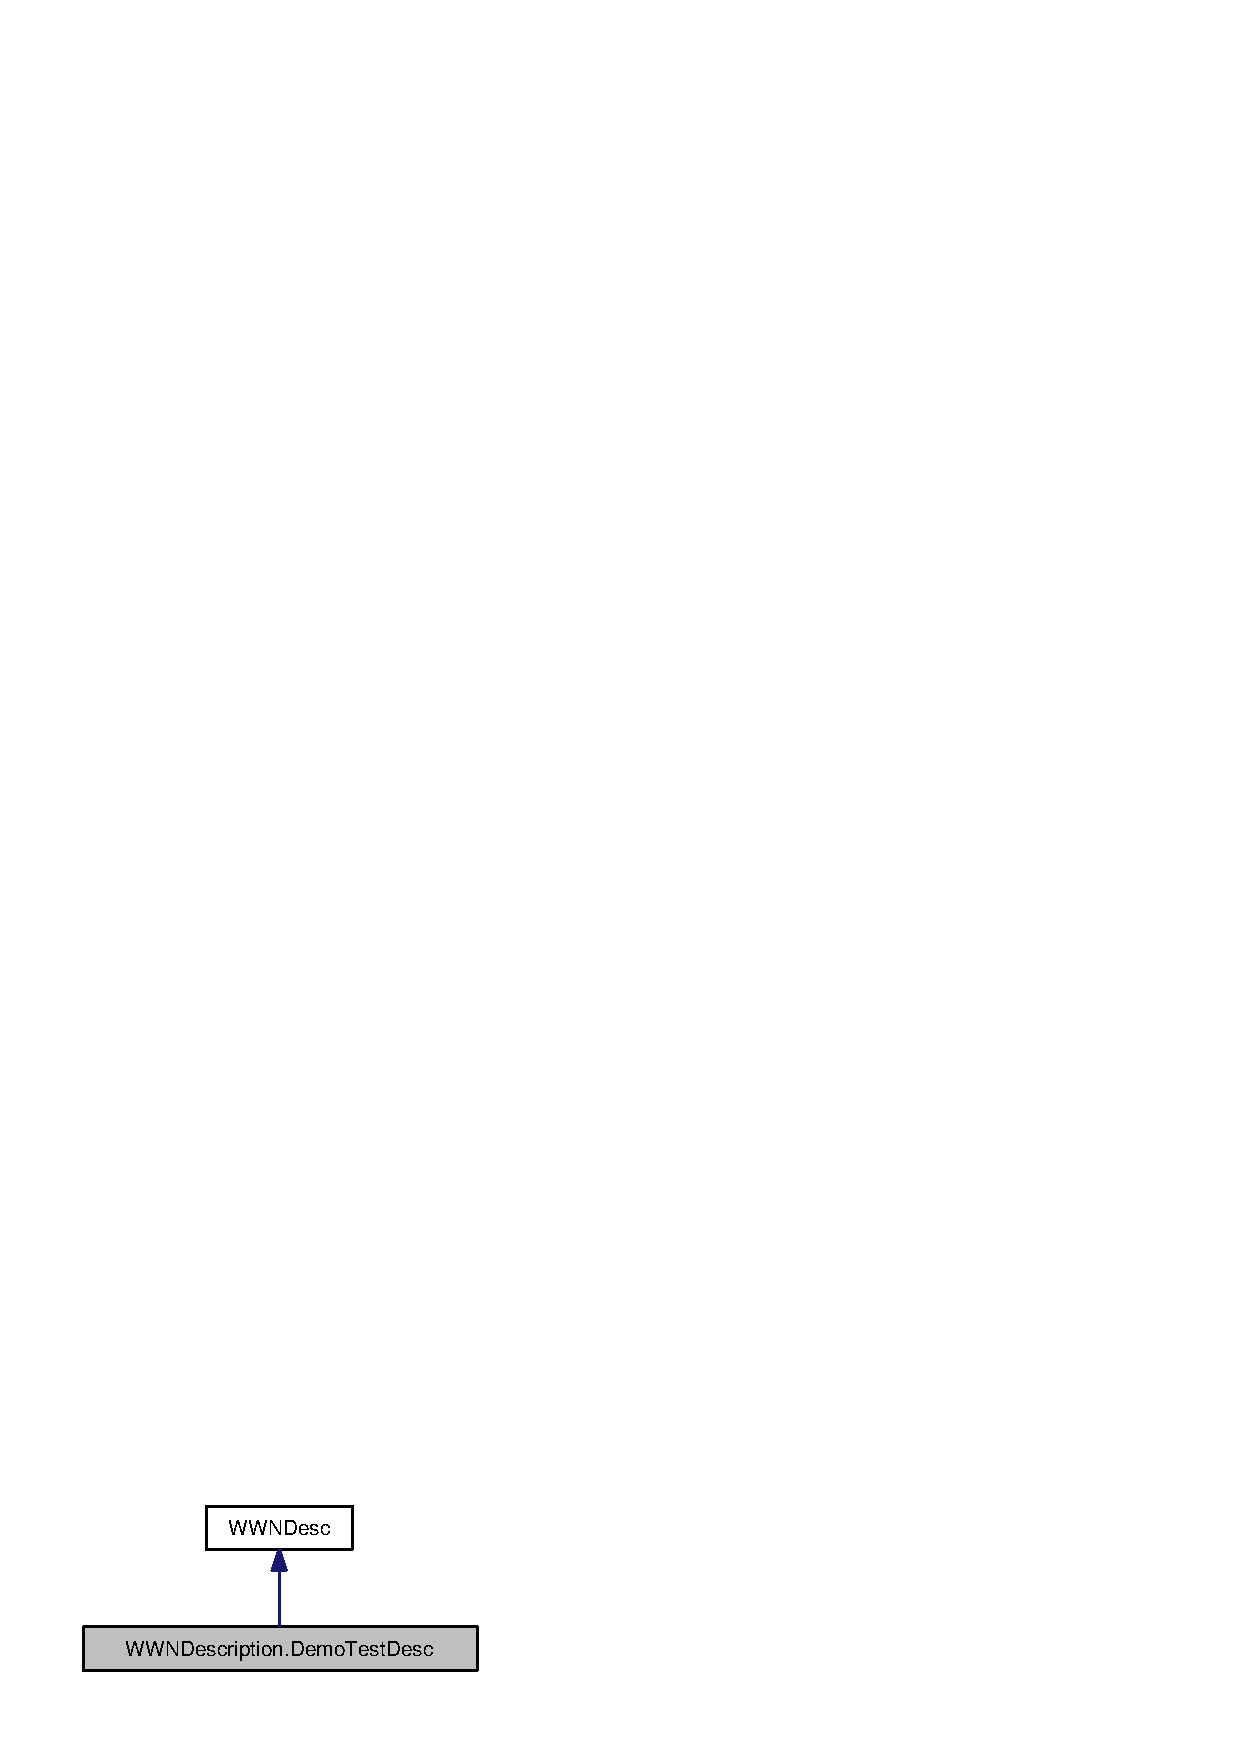
\includegraphics[width=232pt]{classorg_1_1smallfoot_1_1wwn_1_1WWNDescription_1_1DemoTestDesc__inherit__graph}
\end{center}
\end{figure}


Collaboration diagram for W\+W\+N\+Description.\+Demo\+Test\+Desc\+:\nopagebreak
\begin{figure}[H]
\begin{center}
\leavevmode
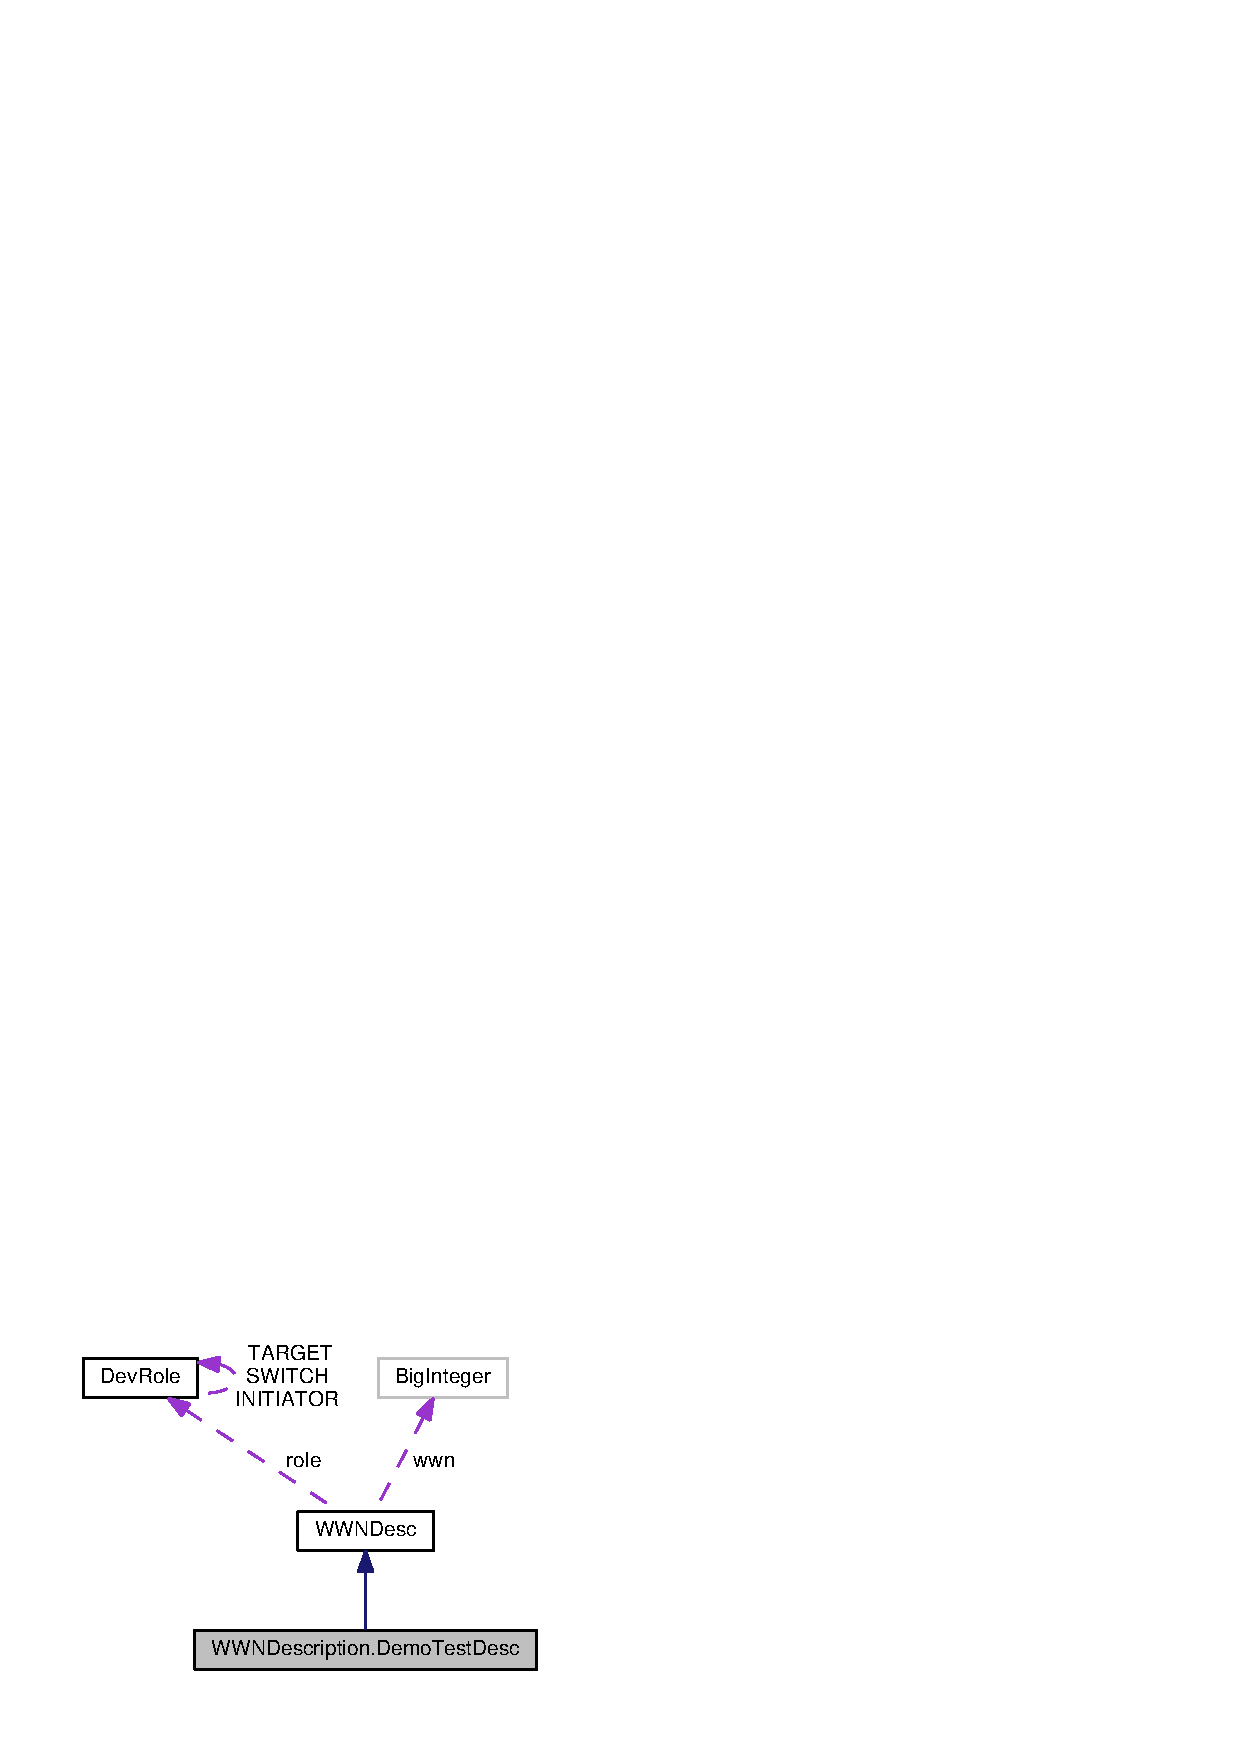
\includegraphics[width=258pt]{classorg_1_1smallfoot_1_1wwn_1_1WWNDescription_1_1DemoTestDesc__coll__graph}
\end{center}
\end{figure}
\subsection*{Public Member Functions}
\begin{DoxyCompactItemize}
\item 
{\bf Demo\+Test\+Desc} (String {\bf wwn})
\begin{DoxyCompactList}\small\item\em create an instance with \doxyref{brief}{p.}{classorg_1_1smallfoot_1_1wwn_1_1WWNDesc_adbebed411e8c47d43338efa3edaa13f8} set to false. \end{DoxyCompactList}\item 
String {\bf to\+String} ()
\begin{DoxyCompactList}\small\item\em generates a test description or alias for this test class \end{DoxyCompactList}\end{DoxyCompactItemize}
\subsection*{Additional Inherited Members}


\subsection{Detailed Description}
test case\+: this matches a single item known to exist in the Demo Database 

Definition at line 34 of file W\+W\+N\+Description.\+java.



\subsection{Constructor \& Destructor Documentation}
\index{org\+::smallfoot\+::wwn\+::\+W\+W\+N\+Description\+::\+Demo\+Test\+Desc@{org\+::smallfoot\+::wwn\+::\+W\+W\+N\+Description\+::\+Demo\+Test\+Desc}!Demo\+Test\+Desc@{Demo\+Test\+Desc}}
\index{Demo\+Test\+Desc@{Demo\+Test\+Desc}!org\+::smallfoot\+::wwn\+::\+W\+W\+N\+Description\+::\+Demo\+Test\+Desc@{org\+::smallfoot\+::wwn\+::\+W\+W\+N\+Description\+::\+Demo\+Test\+Desc}}
\subsubsection[{Demo\+Test\+Desc}]{\setlength{\rightskip}{0pt plus 5cm}{\bf Demo\+Test\+Desc} (
\begin{DoxyParamCaption}
\item[{String}]{wwn}
\end{DoxyParamCaption}
)\hspace{0.3cm}{\ttfamily [inline]}}\label{classorg_1_1smallfoot_1_1wwn_1_1WWNDescription_1_1DemoTestDesc_a20afdb6486eb08bfa269663b13272327}


create an instance with \doxyref{brief}{p.}{classorg_1_1smallfoot_1_1wwn_1_1WWNDesc_adbebed411e8c47d43338efa3edaa13f8} set to false. 

This is a convenience function to support the older constructor model


\begin{DoxyExceptions}{Exceptions}
{\em java.\+lang.\+Null\+Pointer\+Exception} & if the given wwn is null\\
\hline
\end{DoxyExceptions}

\begin{DoxyParams}{Parameters}
{\em wwn} & the W\+W\+N to evaluate and describe \\
\hline
\end{DoxyParams}


Definition at line 37 of file W\+W\+N\+Description.\+java.



\subsection{Member Function Documentation}
\index{org\+::smallfoot\+::wwn\+::\+W\+W\+N\+Description\+::\+Demo\+Test\+Desc@{org\+::smallfoot\+::wwn\+::\+W\+W\+N\+Description\+::\+Demo\+Test\+Desc}!to\+String@{to\+String}}
\index{to\+String@{to\+String}!org\+::smallfoot\+::wwn\+::\+W\+W\+N\+Description\+::\+Demo\+Test\+Desc@{org\+::smallfoot\+::wwn\+::\+W\+W\+N\+Description\+::\+Demo\+Test\+Desc}}
\subsubsection[{to\+String}]{\setlength{\rightskip}{0pt plus 5cm}String to\+String (
\begin{DoxyParamCaption}
{}
\end{DoxyParamCaption}
)\hspace{0.3cm}{\ttfamily [inline]}}\label{classorg_1_1smallfoot_1_1wwn_1_1WWNDescription_1_1DemoTestDesc_ad146fa8579a5f8a876c4688cc5a68520}


generates a test description or alias for this test class 

\begin{DoxyReturn}{Returns}
\char`\"{}\+Test\+Device\char`\"{} always 
\end{DoxyReturn}


Definition at line 46 of file W\+W\+N\+Description.\+java.



The documentation for this class was generated from the following file\+:\begin{DoxyCompactItemize}
\item 
java/{\bf W\+W\+N\+Description.\+java}\end{DoxyCompactItemize}

\section{E\-M\-C\-Clariion\-Description Class Reference}
\label{classorg_1_1smallfoot_1_1wwn_1_1EMCClariionDescription}\index{E\-M\-C\-Clariion\-Description@{E\-M\-C\-Clariion\-Description}}


Inheritance diagram for E\-M\-C\-Clariion\-Description\-:\nopagebreak
\begin{figure}[H]
\begin{center}
\leavevmode
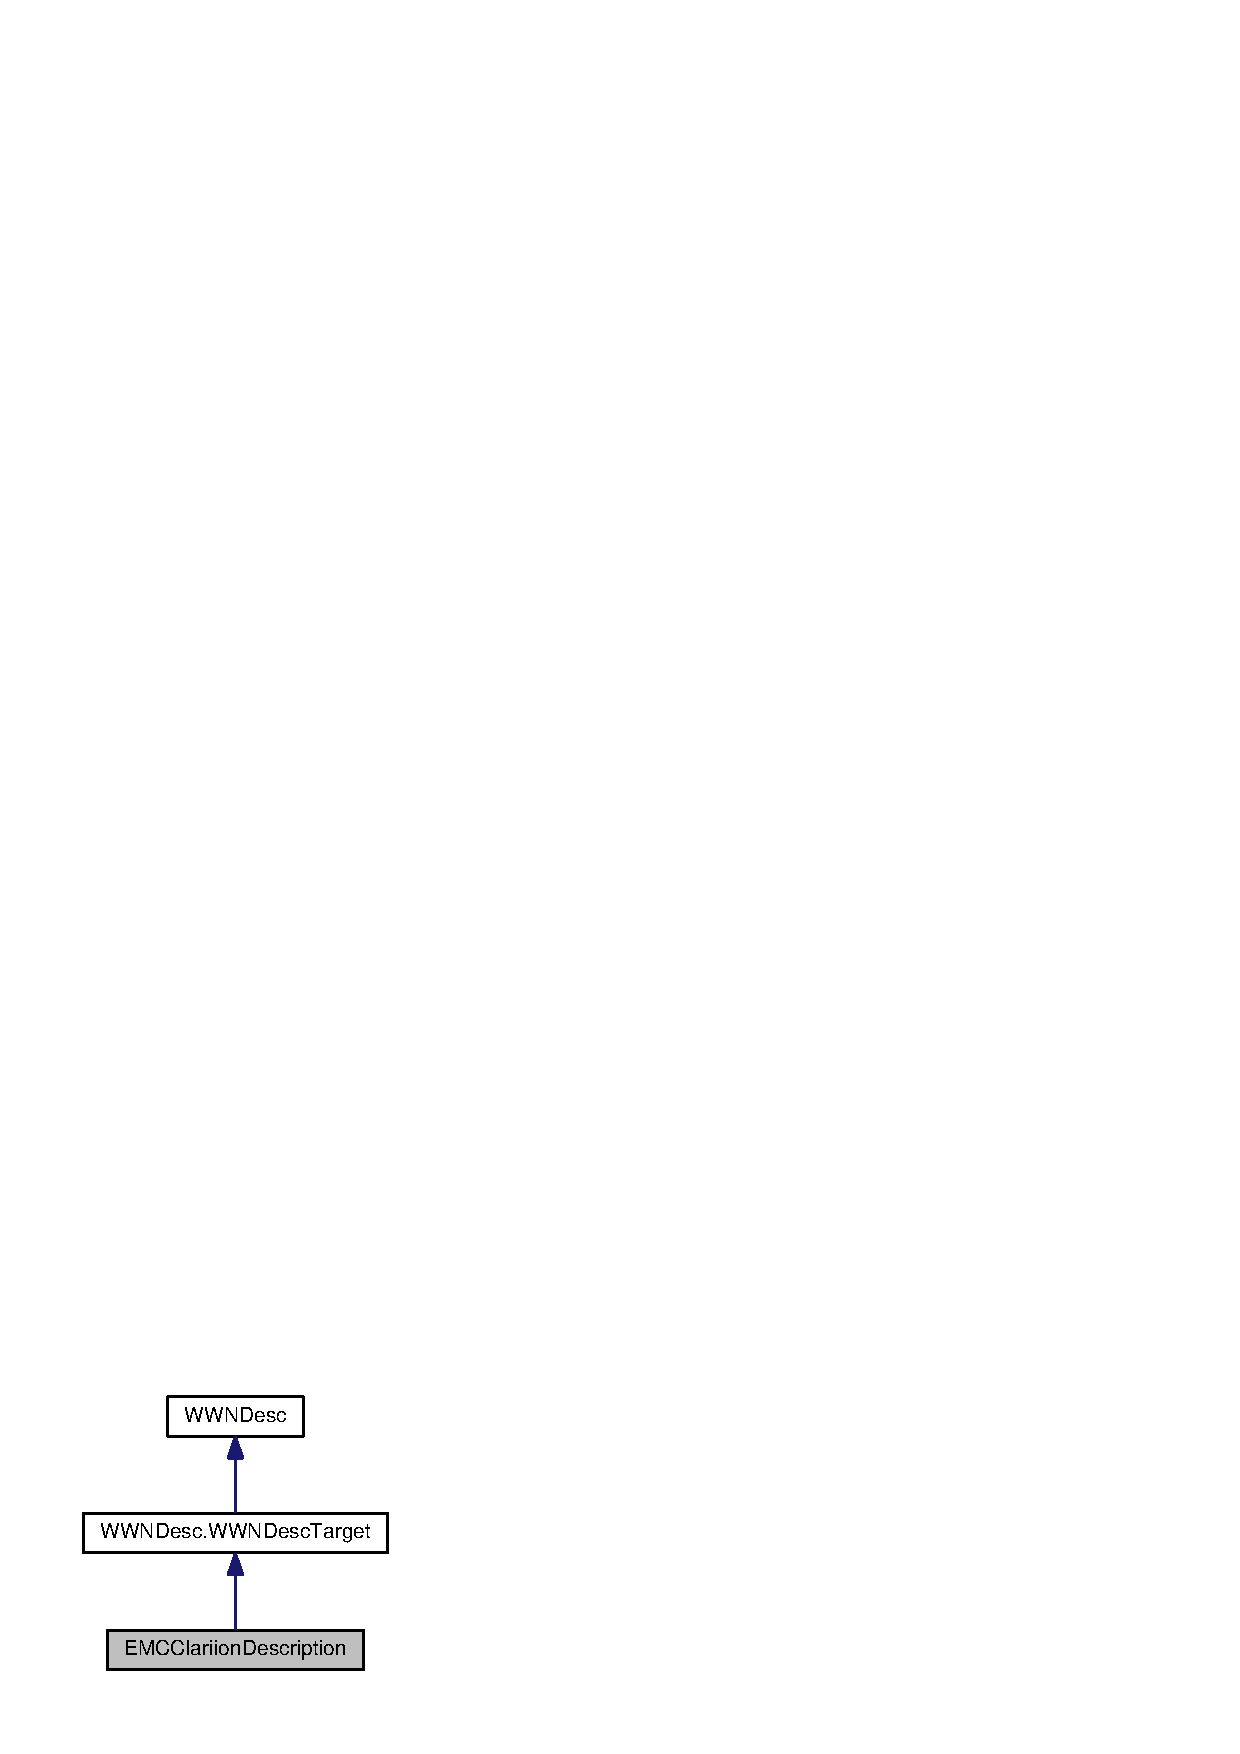
\includegraphics[width=186pt]{classorg_1_1smallfoot_1_1wwn_1_1EMCClariionDescription__inherit__graph}
\end{center}
\end{figure}


Collaboration diagram for E\-M\-C\-Clariion\-Description\-:\nopagebreak
\begin{figure}[H]
\begin{center}
\leavevmode
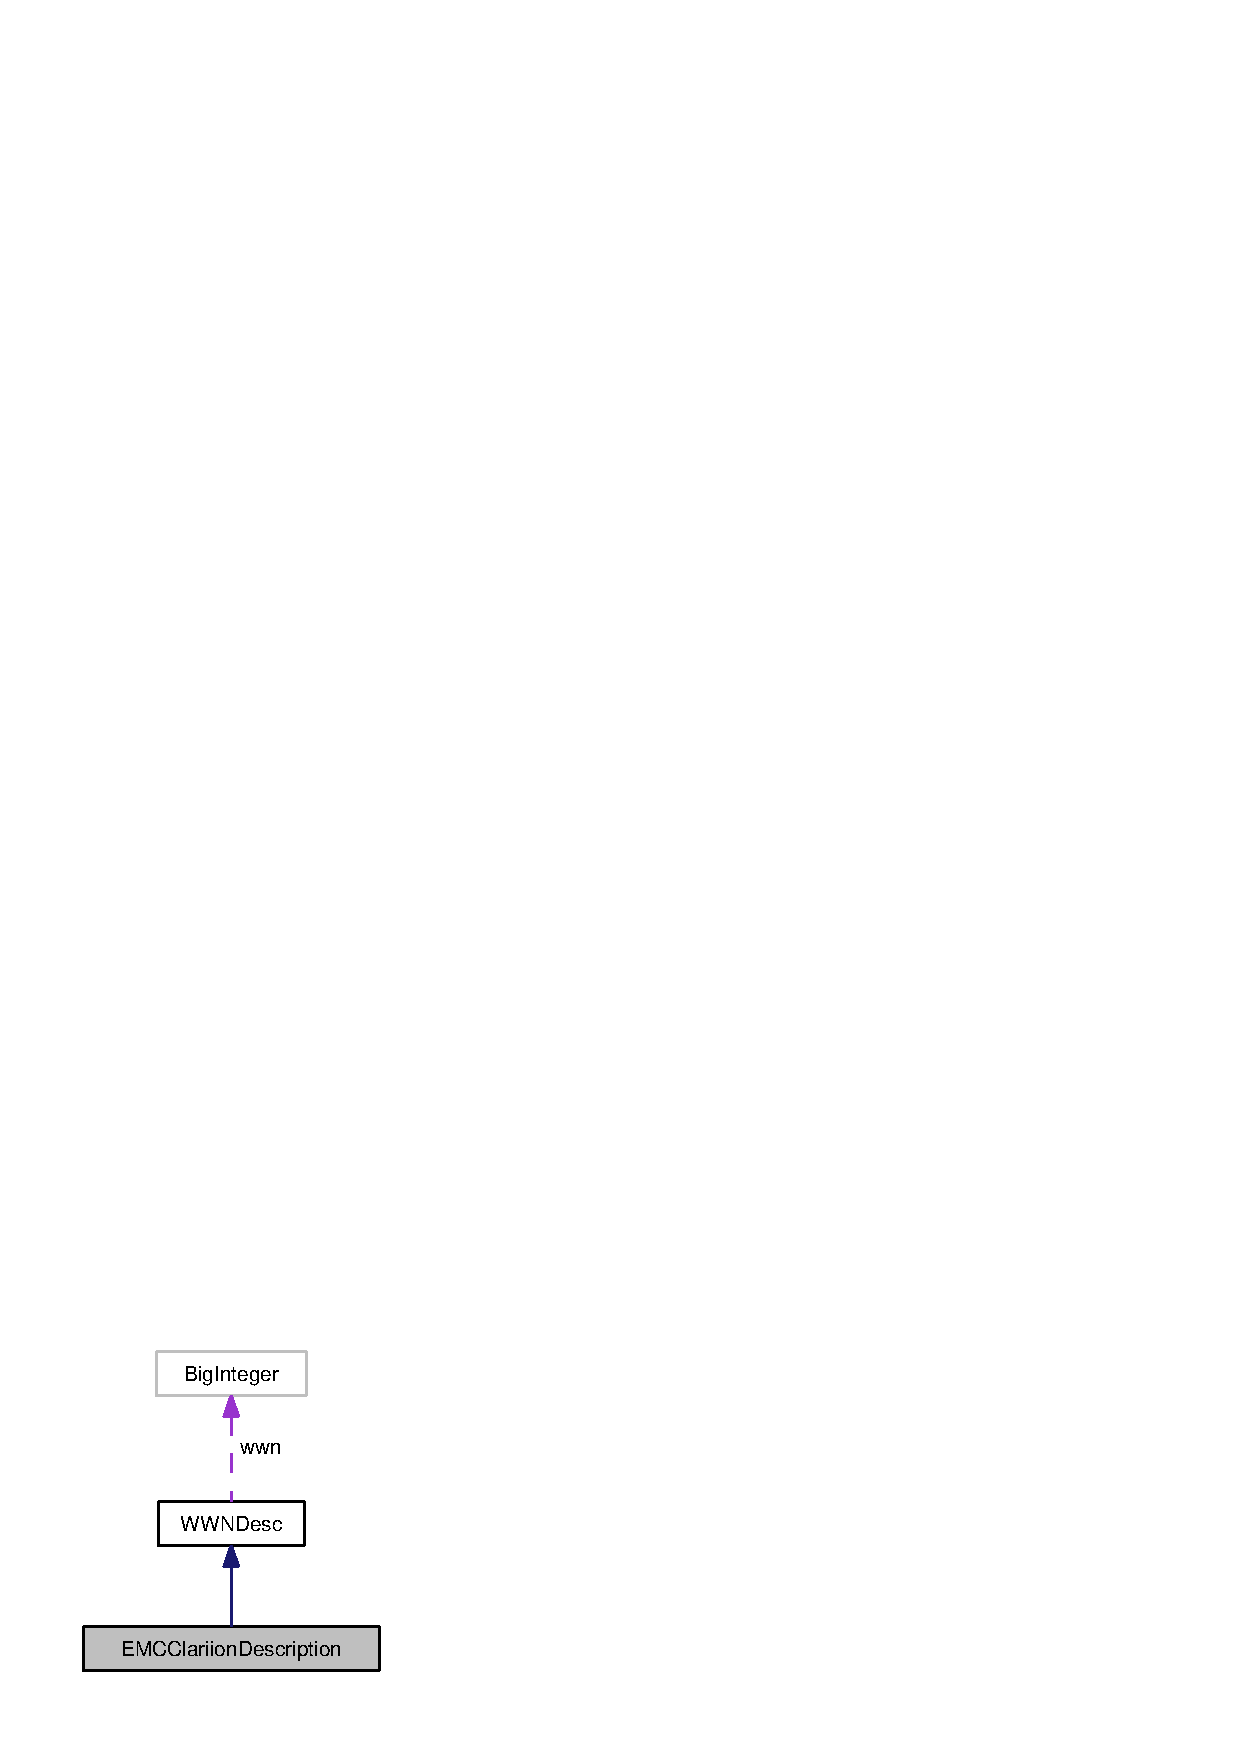
\includegraphics[width=186pt]{classorg_1_1smallfoot_1_1wwn_1_1EMCClariionDescription__coll__graph}
\end{center}
\end{figure}
\subsection*{Public Member Functions}
\begin{DoxyCompactItemize}
\item 
{\bf E\-M\-C\-Clariion\-Description} (String wwn)
\begin{DoxyCompactList}\small\item\em create an instance with this.\-brief set to false. \end{DoxyCompactList}\item 
String {\bf to\-String} ()
\begin{DoxyCompactList}\small\item\em return a description or alias for this W\-W\-N \end{DoxyCompactList}\end{DoxyCompactItemize}
\subsection*{Static Public Member Functions}
\begin{DoxyCompactItemize}
\item 
static {\bf W\-W\-N\-Desc} {\bf get\-Desc} (boolean strong, boolean brief, String wwn)
\begin{DoxyCompactList}\small\item\em If this class matches or describes the given W\-W\-N, returns a new instance of this class loaded with the given W\-W\-N. \end{DoxyCompactList}\end{DoxyCompactItemize}


\subsection{Detailed Description}


Definition at line 10 of file E\-M\-C\-Clariion\-Description.\-java.



\subsection{Constructor \& Destructor Documentation}
\index{org\-::smallfoot\-::wwn\-::\-E\-M\-C\-Clariion\-Description@{org\-::smallfoot\-::wwn\-::\-E\-M\-C\-Clariion\-Description}!E\-M\-C\-Clariion\-Description@{E\-M\-C\-Clariion\-Description}}
\index{E\-M\-C\-Clariion\-Description@{E\-M\-C\-Clariion\-Description}!org::smallfoot::wwn::EMCClariionDescription@{org\-::smallfoot\-::wwn\-::\-E\-M\-C\-Clariion\-Description}}
\subsubsection[{E\-M\-C\-Clariion\-Description}]{\setlength{\rightskip}{0pt plus 5cm}{\bf E\-M\-C\-Clariion\-Description} (
\begin{DoxyParamCaption}
\item[{String}]{wwn}
\end{DoxyParamCaption}
)\hspace{0.3cm}{\ttfamily [inline]}}\label{classorg_1_1smallfoot_1_1wwn_1_1EMCClariionDescription_a6bc5999432db0b6ceae07085b17901f2}


create an instance with this.\-brief set to false. 

This is a convenience function to support the older constructor model


\begin{DoxyParams}{Parameters}
{\em wwn} & the W\-W\-N to evaluate and describe \\
\hline
\end{DoxyParams}


Definition at line 13 of file E\-M\-C\-Clariion\-Description.\-java.



Referenced by E\-M\-C\-Clariion\-Description.\-get\-Desc().



\subsection{Member Function Documentation}
\index{org\-::smallfoot\-::wwn\-::\-E\-M\-C\-Clariion\-Description@{org\-::smallfoot\-::wwn\-::\-E\-M\-C\-Clariion\-Description}!get\-Desc@{get\-Desc}}
\index{get\-Desc@{get\-Desc}!org::smallfoot::wwn::EMCClariionDescription@{org\-::smallfoot\-::wwn\-::\-E\-M\-C\-Clariion\-Description}}
\subsubsection[{get\-Desc}]{\setlength{\rightskip}{0pt plus 5cm}static {\bf W\-W\-N\-Desc} get\-Desc (
\begin{DoxyParamCaption}
\item[{boolean}]{strong, }
\item[{boolean}]{brief, }
\item[{String}]{wwn}
\end{DoxyParamCaption}
)\hspace{0.3cm}{\ttfamily [inline]}, {\ttfamily [static]}}\label{classorg_1_1smallfoot_1_1wwn_1_1EMCClariionDescription_a7e34be4d9bd11a9971c007c6231b8c01}


If this class matches or describes the given W\-W\-N, returns a new instance of this class loaded with the given W\-W\-N. 

\begin{DoxyReturn}{Returns}
new instance of this class, or null if the given wwn does not match this class 
\end{DoxyReturn}

\begin{DoxyParams}{Parameters}
{\em strong} & is ignored\-: this class is a strong representation, not a weak one based on empirical matching, hence can always be used with confidence \\
\hline
{\em brief} & is ignored\-: this class has only one representation of the W\-W\-N description or alias \\
\hline
{\em wwn} & the W\-W\-N (W\-W\-P\-N or W\-W\-N\-N, but typically W\-W\-P\-N) to match \\
\hline
\end{DoxyParams}


Definition at line 26 of file E\-M\-C\-Clariion\-Description.\-java.



References E\-M\-C\-Clariion\-Description.\-E\-M\-C\-Clariion\-Description().



Referenced by W\-W\-N\-Description.\-get\-W\-W\-N\-Descriptor().



Here is the call graph for this function\-:\nopagebreak
\begin{figure}[H]
\begin{center}
\leavevmode
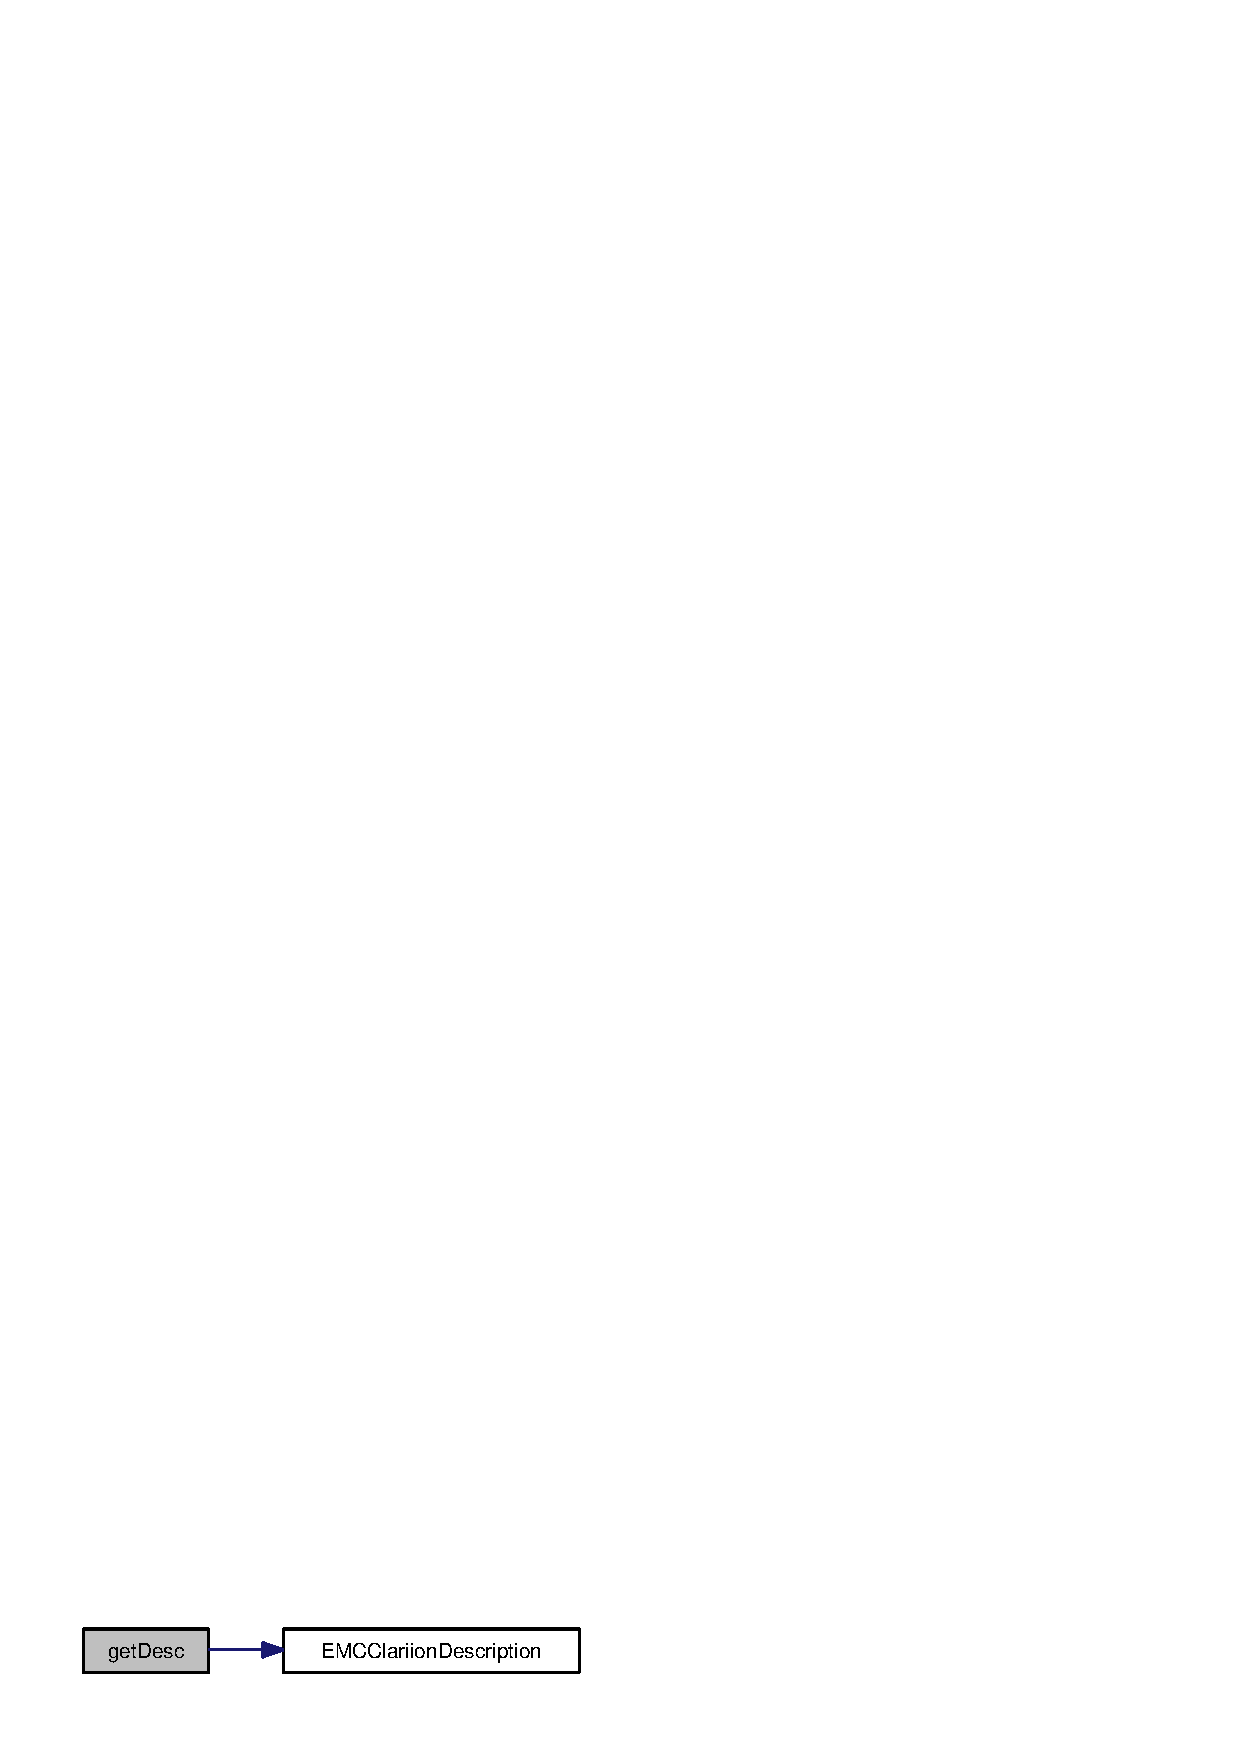
\includegraphics[width=282pt]{classorg_1_1smallfoot_1_1wwn_1_1EMCClariionDescription_a7e34be4d9bd11a9971c007c6231b8c01_cgraph}
\end{center}
\end{figure}


\index{org\-::smallfoot\-::wwn\-::\-E\-M\-C\-Clariion\-Description@{org\-::smallfoot\-::wwn\-::\-E\-M\-C\-Clariion\-Description}!to\-String@{to\-String}}
\index{to\-String@{to\-String}!org::smallfoot::wwn::EMCClariionDescription@{org\-::smallfoot\-::wwn\-::\-E\-M\-C\-Clariion\-Description}}
\subsubsection[{to\-String}]{\setlength{\rightskip}{0pt plus 5cm}String to\-String (
\begin{DoxyParamCaption}
{}
\end{DoxyParamCaption}
)\hspace{0.3cm}{\ttfamily [inline]}}\label{classorg_1_1smallfoot_1_1wwn_1_1EMCClariionDescription_ad146fa8579a5f8a876c4688cc5a68520}


return a description or alias for this W\-W\-N 

\begin{DoxyReturn}{Returns}
generated alias or nickname for the W\-W\-N 
\end{DoxyReturn}


Definition at line 39 of file E\-M\-C\-Clariion\-Description.\-java.



The documentation for this class was generated from the following file\-:\begin{DoxyCompactItemize}
\item 
java/{\bf E\-M\-C\-Clariion\-Description.\-java}\end{DoxyCompactItemize}

\section{E\+M\+C\+Symmetrix\+Description Class Reference}
\label{classorg_1_1smallfoot_1_1wwn_1_1EMCSymmetrixDescription}\index{E\+M\+C\+Symmetrix\+Description@{E\+M\+C\+Symmetrix\+Description}}


\doxyref{E\+M\+C\+Symmetrix\+Description}{p.}{classorg_1_1smallfoot_1_1wwn_1_1EMCSymmetrixDescription} (ie Symm-\/187900328-\/03d\+B or Symm-\/0328-\/03d\+B) breaks out the serial and F\+A port from the W\+W\+P\+N.  




Inheritance diagram for E\+M\+C\+Symmetrix\+Description\+:\nopagebreak
\begin{figure}[H]
\begin{center}
\leavevmode
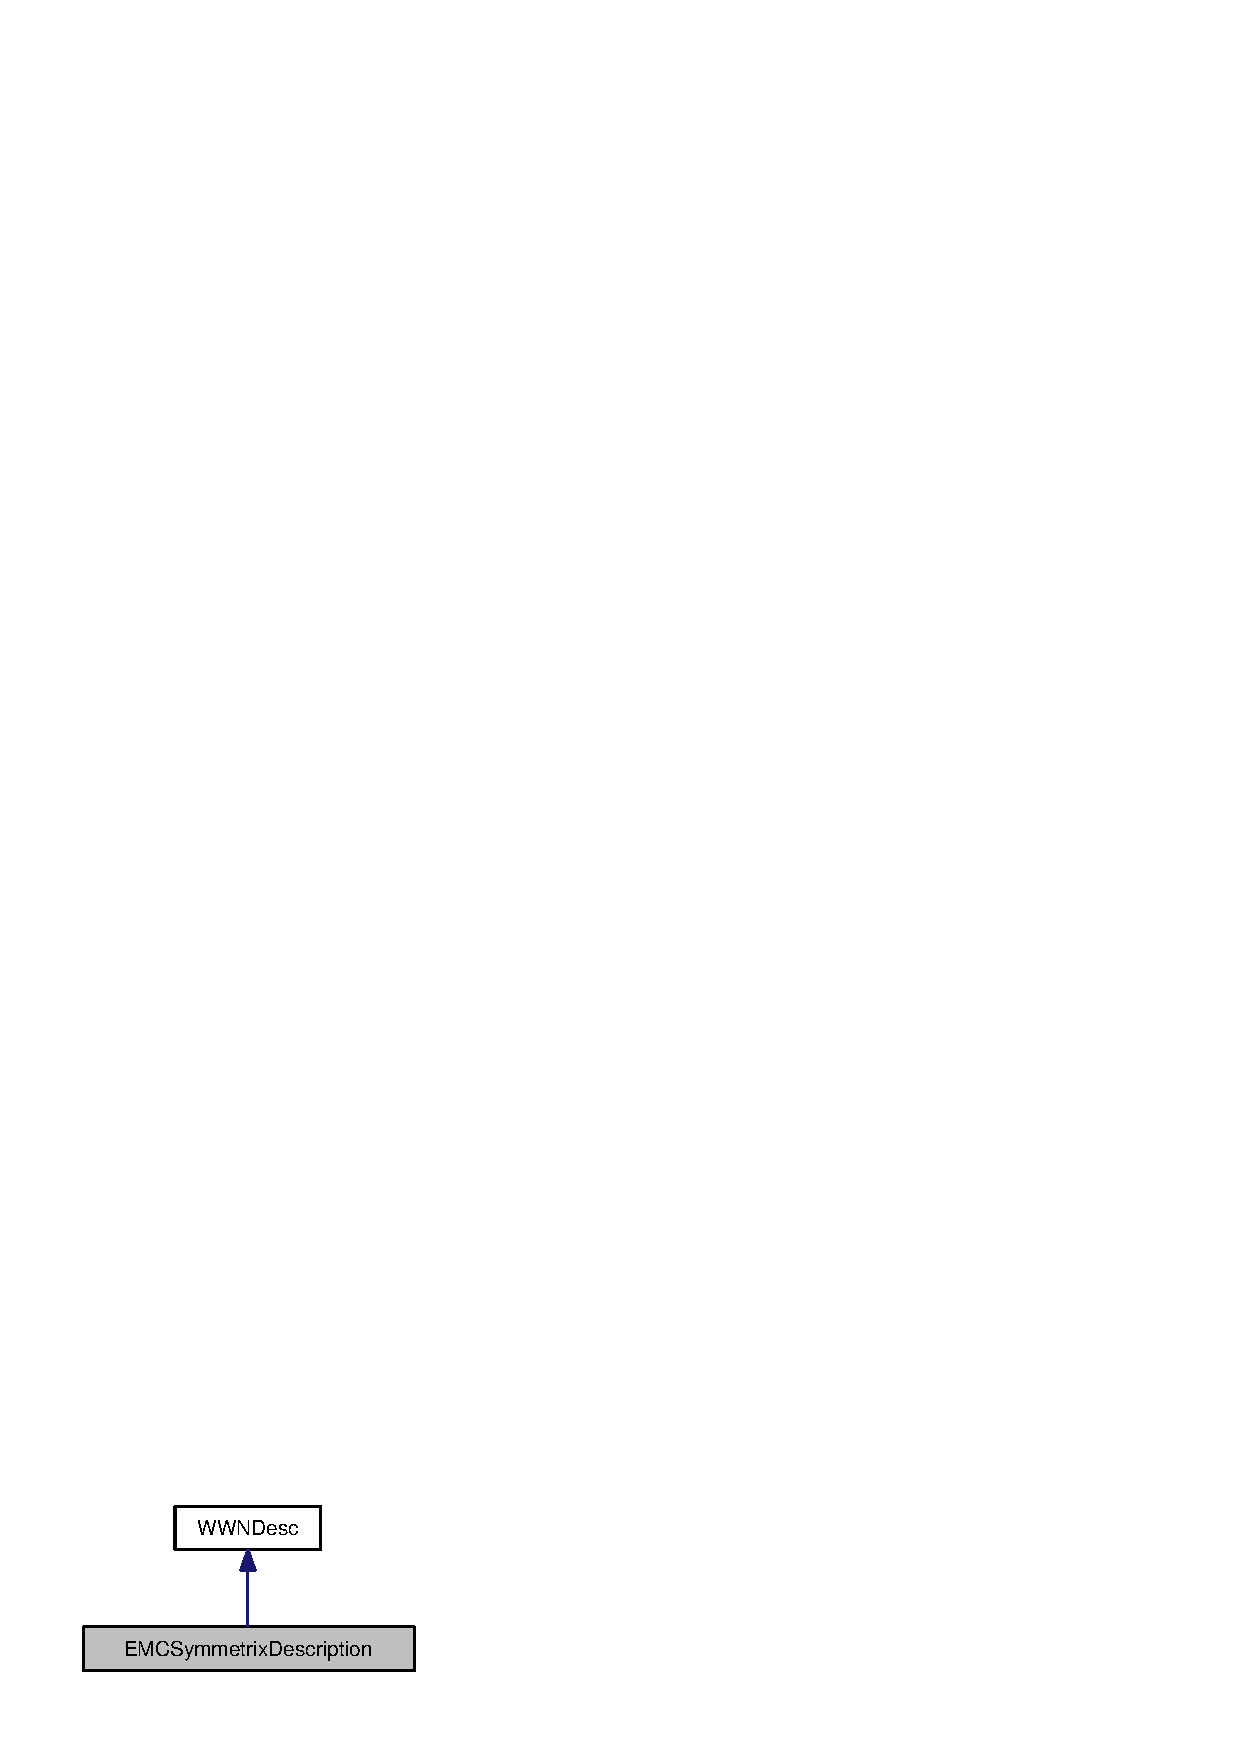
\includegraphics[width=188pt]{classorg_1_1smallfoot_1_1wwn_1_1EMCSymmetrixDescription__inherit__graph}
\end{center}
\end{figure}


Collaboration diagram for E\+M\+C\+Symmetrix\+Description\+:\nopagebreak
\begin{figure}[H]
\begin{center}
\leavevmode
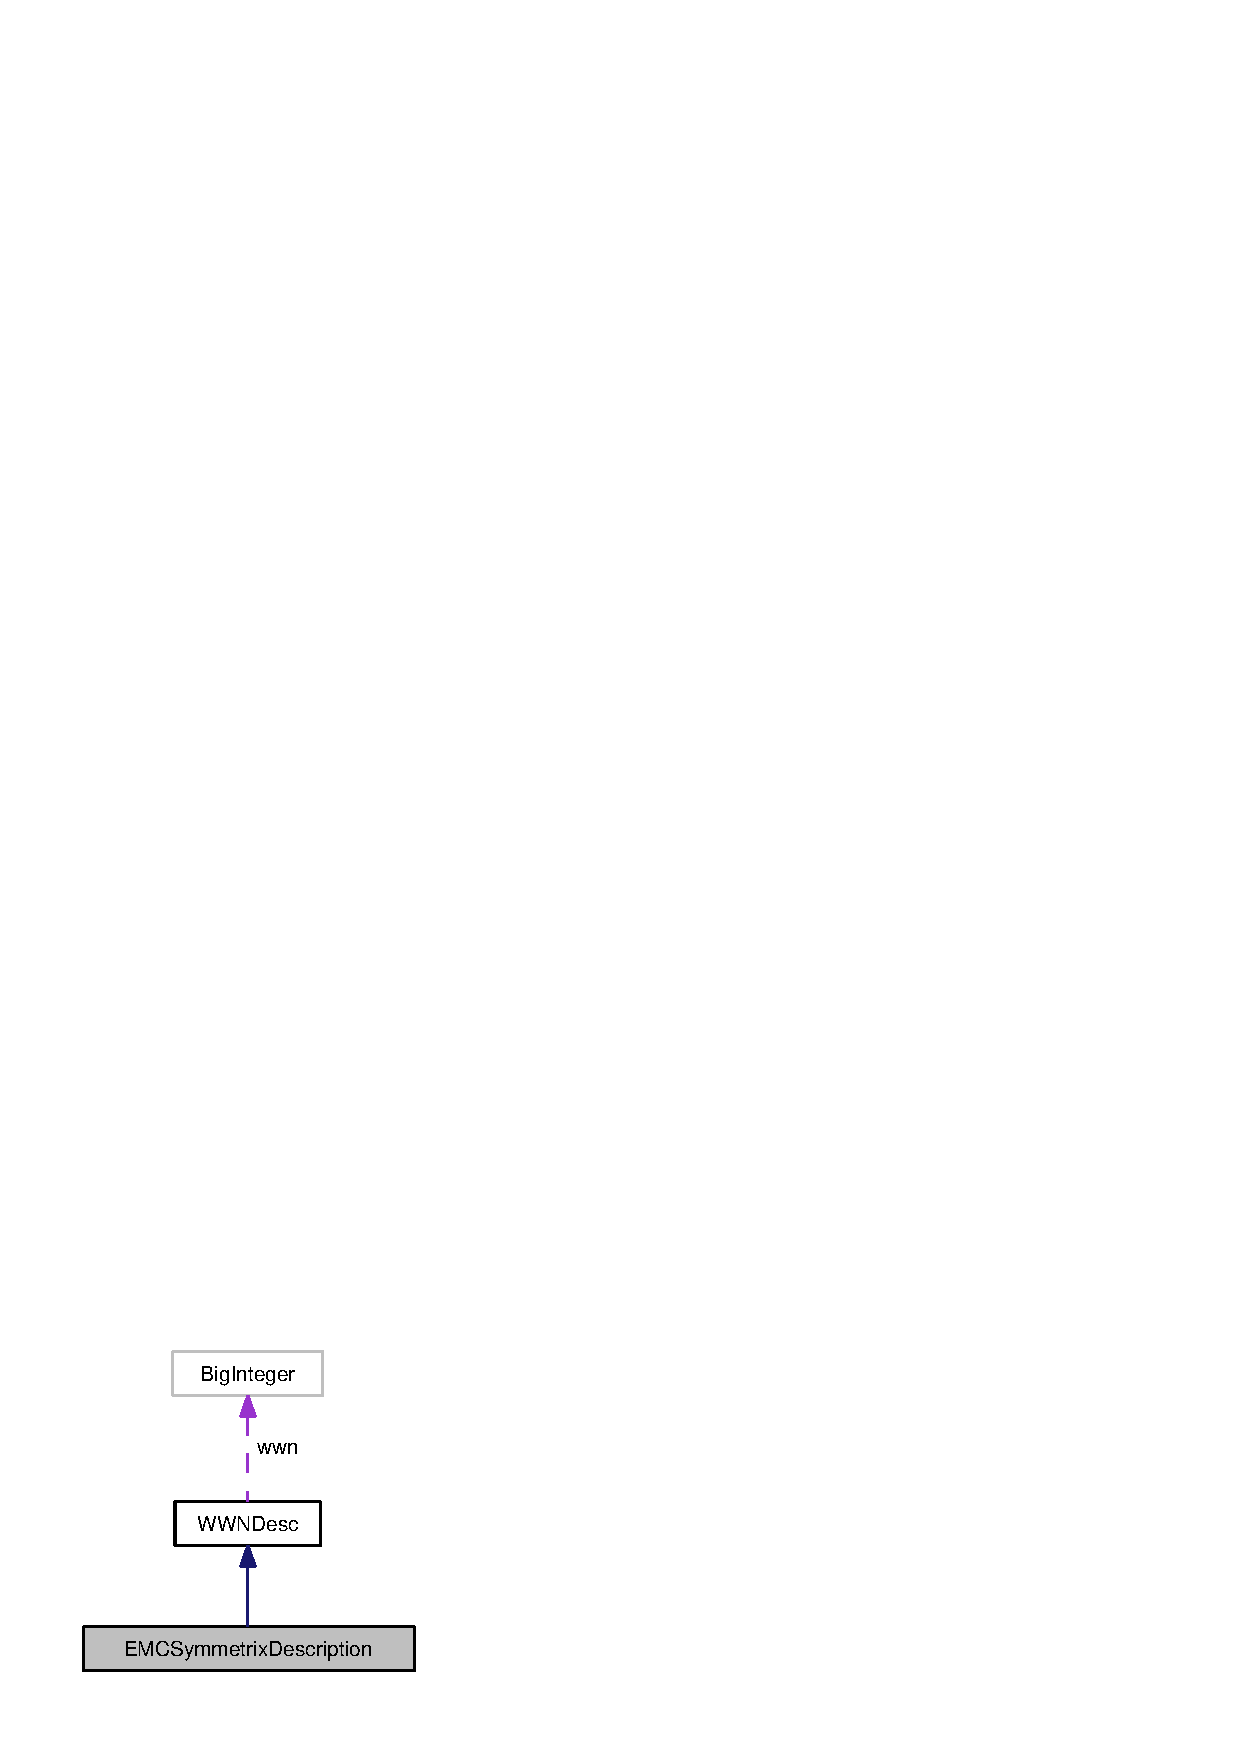
\includegraphics[width=249pt]{classorg_1_1smallfoot_1_1wwn_1_1EMCSymmetrixDescription__coll__graph}
\end{center}
\end{figure}
\subsection*{Public Member Functions}
\begin{DoxyCompactItemize}
\item 
{\bf E\+M\+C\+Symmetrix\+Description} (String {\bf wwn})
\begin{DoxyCompactList}\small\item\em create an instance with \doxyref{brief}{p.}{classorg_1_1smallfoot_1_1wwn_1_1WWNDesc_adbebed411e8c47d43338efa3edaa13f8} set to false. \end{DoxyCompactList}\item 
{\bf E\+M\+C\+Symmetrix\+Description} (boolean {\bf brief}, String {\bf wwn})
\begin{DoxyCompactList}\small\item\em create an instance with the given W\+W\+N. \end{DoxyCompactList}\item 
String {\bf to\+String} ()
\begin{DoxyCompactList}\small\item\em return a description or alias for this W\+W\+N; if brief is set to true during the call to \doxyref{get\+Desc()}{p.}{classorg_1_1smallfoot_1_1wwn_1_1EMCSymmetrixDescription_a7e34be4d9bd11a9971c007c6231b8c01}, then a shorter description or alias will be returned \end{DoxyCompactList}\end{DoxyCompactItemize}
\subsection*{Static Public Member Functions}
\begin{DoxyCompactItemize}
\item 
static {\bf W\+W\+N\+Desc} {\bf get\+Desc} (boolean strong, boolean {\bf brief}, String {\bf wwn})
\begin{DoxyCompactList}\small\item\em If this class matches or describes the given W\+W\+N, returns a new instance of this class loaded with the given W\+W\+N. \end{DoxyCompactList}\item 
static {\bf W\+W\+N\+Desc} {\bf get\+Desc} (boolean strong, boolean {\bf brief}, String {\bf wwn}, int {\bf role})
\begin{DoxyCompactList}\small\item\em If this class matches or describes the given W\+W\+N, returns a new instance of this class loaded with the given W\+W\+N. \end{DoxyCompactList}\end{DoxyCompactItemize}
\subsection*{Additional Inherited Members}


\subsection{Detailed Description}
\doxyref{E\+M\+C\+Symmetrix\+Description}{p.}{classorg_1_1smallfoot_1_1wwn_1_1EMCSymmetrixDescription} (ie Symm-\/187900328-\/03d\+B or Symm-\/0328-\/03d\+B) breaks out the serial and F\+A port from the W\+W\+P\+N. 

\begin{DoxySeeAlso}{See also}
\doxyref{E\+M\+C\+Symmetrix\+Description}{p.}{classorg_1_1smallfoot_1_1wwn_1_1EMCSymmetrixDescription} 

\doxyref{E\+M\+C\+V\+M\+A\+X\+Description}{p.}{classorg_1_1smallfoot_1_1wwn_1_1EMCVMAXDescription} 

\doxyref{E\+M\+C\+V\+P\+L\+E\+X\+Description}{p.}{classorg_1_1smallfoot_1_1wwn_1_1EMCVPLEXDescription} 
\end{DoxySeeAlso}


Definition at line 13 of file E\+M\+C\+Symmetrix\+Description.\+java.



\subsection{Constructor \& Destructor Documentation}
\index{org\+::smallfoot\+::wwn\+::\+E\+M\+C\+Symmetrix\+Description@{org\+::smallfoot\+::wwn\+::\+E\+M\+C\+Symmetrix\+Description}!E\+M\+C\+Symmetrix\+Description@{E\+M\+C\+Symmetrix\+Description}}
\index{E\+M\+C\+Symmetrix\+Description@{E\+M\+C\+Symmetrix\+Description}!org\+::smallfoot\+::wwn\+::\+E\+M\+C\+Symmetrix\+Description@{org\+::smallfoot\+::wwn\+::\+E\+M\+C\+Symmetrix\+Description}}
\subsubsection[{E\+M\+C\+Symmetrix\+Description}]{\setlength{\rightskip}{0pt plus 5cm}{\bf E\+M\+C\+Symmetrix\+Description} (
\begin{DoxyParamCaption}
\item[{String}]{wwn}
\end{DoxyParamCaption}
)\hspace{0.3cm}{\ttfamily [inline]}}\label{classorg_1_1smallfoot_1_1wwn_1_1EMCSymmetrixDescription_aac54d649a6df7c45f2e0424649a6acdd}


create an instance with \doxyref{brief}{p.}{classorg_1_1smallfoot_1_1wwn_1_1WWNDesc_adbebed411e8c47d43338efa3edaa13f8} set to false. 

This is a convenience function to support the older constructor model


\begin{DoxyExceptions}{Exceptions}
{\em java.\+lang.\+Null\+Pointer\+Exception} & if the given wwn is null\\
\hline
\end{DoxyExceptions}

\begin{DoxyParams}{Parameters}
{\em wwn} & the W\+W\+N to evaluate and describe \\
\hline
\end{DoxyParams}


Definition at line 16 of file E\+M\+C\+Symmetrix\+Description.\+java.



Referenced by E\+M\+C\+Symmetrix\+Description.\+get\+Desc().

\index{org\+::smallfoot\+::wwn\+::\+E\+M\+C\+Symmetrix\+Description@{org\+::smallfoot\+::wwn\+::\+E\+M\+C\+Symmetrix\+Description}!E\+M\+C\+Symmetrix\+Description@{E\+M\+C\+Symmetrix\+Description}}
\index{E\+M\+C\+Symmetrix\+Description@{E\+M\+C\+Symmetrix\+Description}!org\+::smallfoot\+::wwn\+::\+E\+M\+C\+Symmetrix\+Description@{org\+::smallfoot\+::wwn\+::\+E\+M\+C\+Symmetrix\+Description}}
\subsubsection[{E\+M\+C\+Symmetrix\+Description}]{\setlength{\rightskip}{0pt plus 5cm}{\bf E\+M\+C\+Symmetrix\+Description} (
\begin{DoxyParamCaption}
\item[{boolean}]{brief, }
\item[{String}]{wwn}
\end{DoxyParamCaption}
)\hspace{0.3cm}{\ttfamily [inline]}}\label{classorg_1_1smallfoot_1_1wwn_1_1EMCSymmetrixDescription_a52f4d3c2e88500ffbfc0a611ac75df5b}


create an instance with the given W\+W\+N. 

Values given to the constructor are simply copied to internal variables for later use


\begin{DoxyExceptions}{Exceptions}
{\em java.\+lang.\+Null\+Pointer\+Exception} & if the given wwn is null\\
\hline
\end{DoxyExceptions}

\begin{DoxyParams}{Parameters}
{\em brief} & whether an abbreviated description is requested \\
\hline
{\em wwn} & the W\+W\+N to evaluate and describe \\
\hline
\end{DoxyParams}


Definition at line 21 of file E\+M\+C\+Symmetrix\+Description.\+java.



\subsection{Member Function Documentation}
\index{org\+::smallfoot\+::wwn\+::\+E\+M\+C\+Symmetrix\+Description@{org\+::smallfoot\+::wwn\+::\+E\+M\+C\+Symmetrix\+Description}!get\+Desc@{get\+Desc}}
\index{get\+Desc@{get\+Desc}!org\+::smallfoot\+::wwn\+::\+E\+M\+C\+Symmetrix\+Description@{org\+::smallfoot\+::wwn\+::\+E\+M\+C\+Symmetrix\+Description}}
\subsubsection[{get\+Desc}]{\setlength{\rightskip}{0pt plus 5cm}static {\bf W\+W\+N\+Desc} get\+Desc (
\begin{DoxyParamCaption}
\item[{boolean}]{strong, }
\item[{boolean}]{brief, }
\item[{String}]{wwn}
\end{DoxyParamCaption}
)\hspace{0.3cm}{\ttfamily [inline]}, {\ttfamily [static]}}\label{classorg_1_1smallfoot_1_1wwn_1_1EMCSymmetrixDescription_a7e34be4d9bd11a9971c007c6231b8c01}


If this class matches or describes the given W\+W\+N, returns a new instance of this class loaded with the given W\+W\+N. 

\begin{DoxyReturn}{Returns}
new instance of this class, or null if the given wwn does not match this class 
\end{DoxyReturn}

\begin{DoxyParams}{Parameters}
{\em strong} & is ignored\+: this class is a strong representation, not a weak one based on empirical matching, hence can always be used with confidence \\
\hline
{\em brief} & is used to ask for a shorter description\+: a more concise nickname or alias \\
\hline
{\em wwn} & the W\+W\+N (W\+W\+P\+N or W\+W\+N\+N, but typically W\+W\+P\+N) to match \\
\hline
\end{DoxyParams}


Definition at line 34 of file E\+M\+C\+Symmetrix\+Description.\+java.



References Dev\+Role.\+max.



Referenced by W\+W\+N\+Description.\+get\+W\+W\+N\+Descriptor().

\index{org\+::smallfoot\+::wwn\+::\+E\+M\+C\+Symmetrix\+Description@{org\+::smallfoot\+::wwn\+::\+E\+M\+C\+Symmetrix\+Description}!get\+Desc@{get\+Desc}}
\index{get\+Desc@{get\+Desc}!org\+::smallfoot\+::wwn\+::\+E\+M\+C\+Symmetrix\+Description@{org\+::smallfoot\+::wwn\+::\+E\+M\+C\+Symmetrix\+Description}}
\subsubsection[{get\+Desc}]{\setlength{\rightskip}{0pt plus 5cm}static {\bf W\+W\+N\+Desc} get\+Desc (
\begin{DoxyParamCaption}
\item[{boolean}]{strong, }
\item[{boolean}]{brief, }
\item[{String}]{wwn, }
\item[{int}]{role}
\end{DoxyParamCaption}
)\hspace{0.3cm}{\ttfamily [inline]}, {\ttfamily [static]}}\label{classorg_1_1smallfoot_1_1wwn_1_1EMCSymmetrixDescription_a37ac294533314b3b7b3a5f3404ee43d6}


If this class matches or describes the given W\+W\+N, returns a new instance of this class loaded with the given W\+W\+N. 

\begin{DoxyReturn}{Returns}
new instance of this class, or null if the given wwn does not match this class 
\end{DoxyReturn}

\begin{DoxyParams}{Parameters}
{\em strong} & is ignored\+: this class is a strong representation, not a weak one based on empirical matching, hence can always be used with confidence \\
\hline
{\em brief} & is used to ask for a shorter description\+: a more concise nickname or alias \\
\hline
{\em wwn} & the W\+W\+N (W\+W\+P\+N or W\+W\+N\+N, but typically W\+W\+P\+N) to match \\
\hline
{\em role} & Role (Initiator/\+Switch/\+Target) to check for \\
\hline
\end{DoxyParams}


Definition at line 42 of file E\+M\+C\+Symmetrix\+Description.\+java.



References E\+M\+C\+Symmetrix\+Description.\+E\+M\+C\+Symmetrix\+Description(), and W\+W\+N\+Desc.\+W\+W\+N\+Desc\+Target.\+is\+A().



Here is the call graph for this function\+:\nopagebreak
\begin{figure}[H]
\begin{center}
\leavevmode
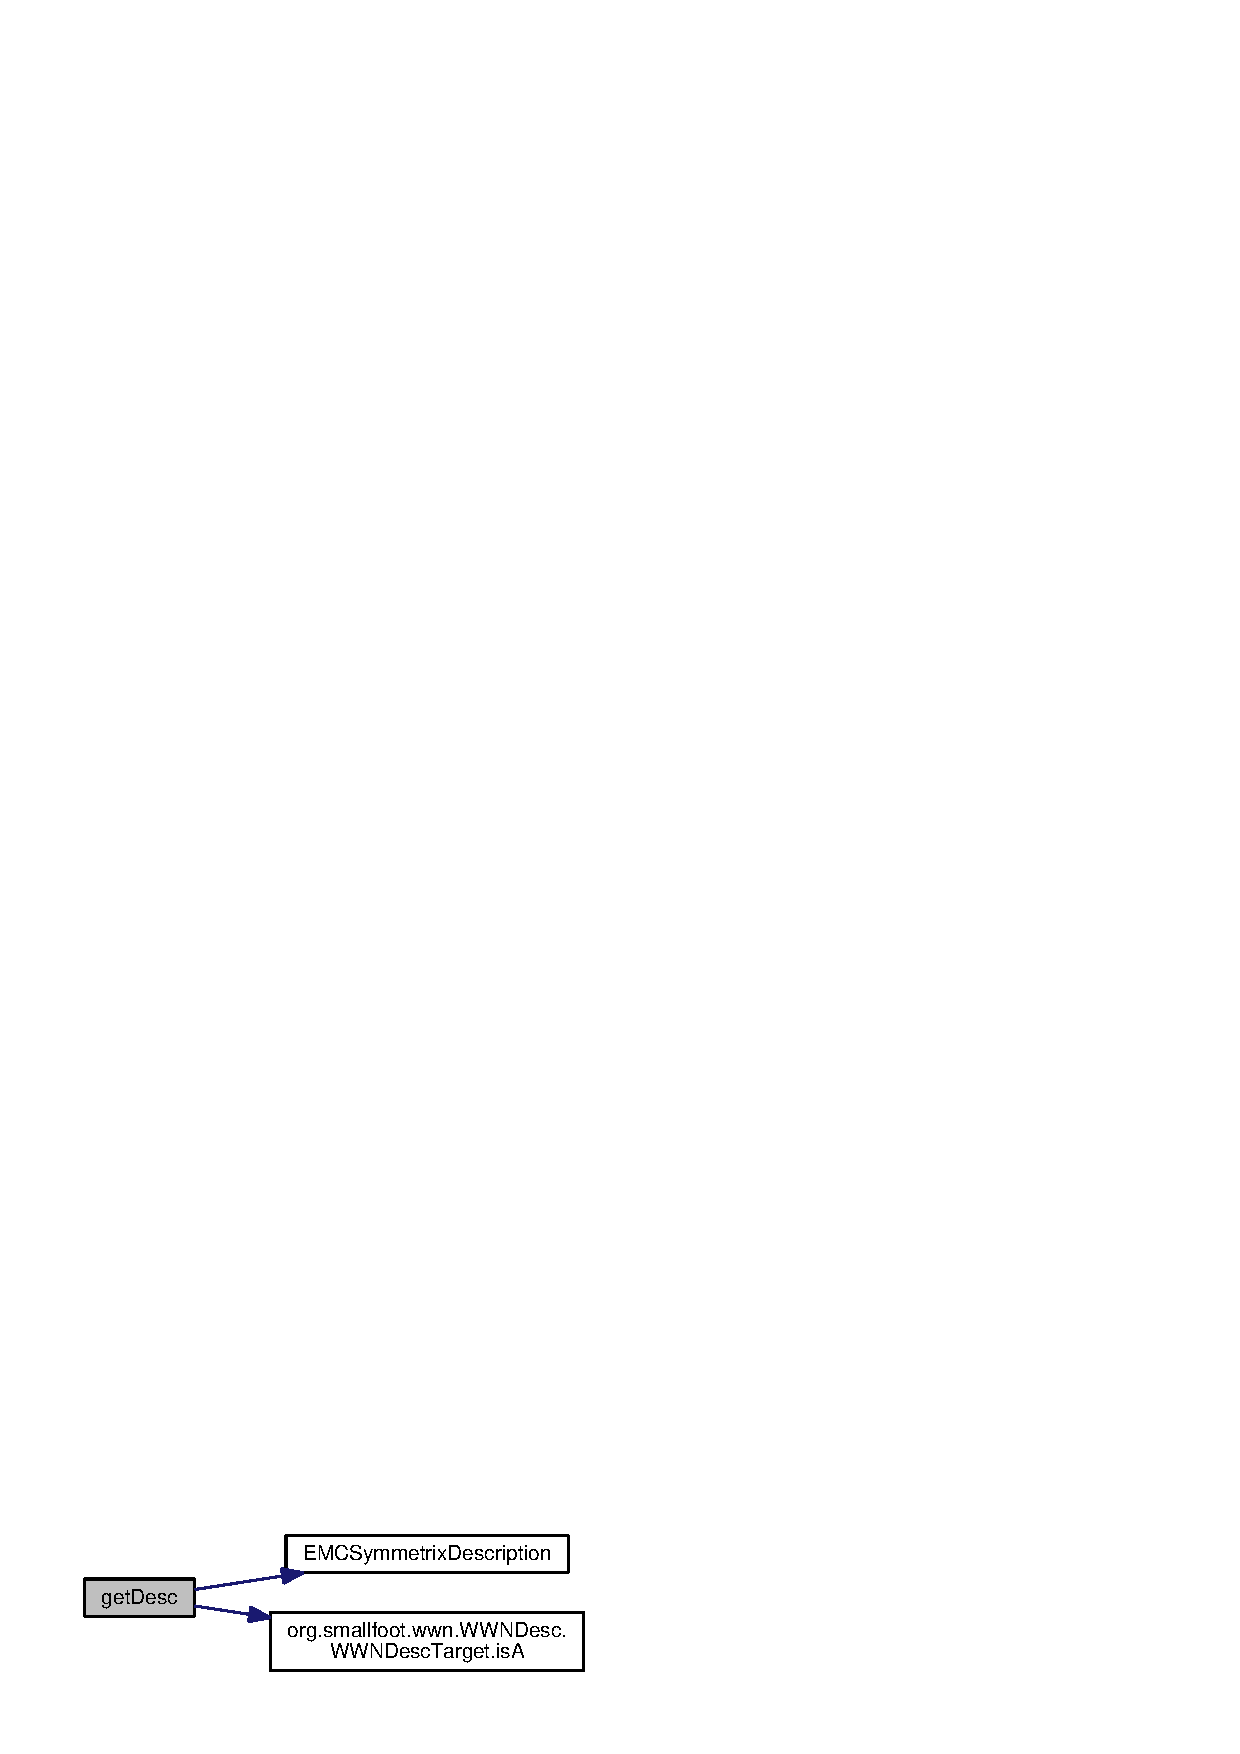
\includegraphics[width=284pt]{classorg_1_1smallfoot_1_1wwn_1_1EMCSymmetrixDescription_a37ac294533314b3b7b3a5f3404ee43d6_cgraph}
\end{center}
\end{figure}


\index{org\+::smallfoot\+::wwn\+::\+E\+M\+C\+Symmetrix\+Description@{org\+::smallfoot\+::wwn\+::\+E\+M\+C\+Symmetrix\+Description}!to\+String@{to\+String}}
\index{to\+String@{to\+String}!org\+::smallfoot\+::wwn\+::\+E\+M\+C\+Symmetrix\+Description@{org\+::smallfoot\+::wwn\+::\+E\+M\+C\+Symmetrix\+Description}}
\subsubsection[{to\+String}]{\setlength{\rightskip}{0pt plus 5cm}String to\+String (
\begin{DoxyParamCaption}
{}
\end{DoxyParamCaption}
)\hspace{0.3cm}{\ttfamily [inline]}}\label{classorg_1_1smallfoot_1_1wwn_1_1EMCSymmetrixDescription_ad146fa8579a5f8a876c4688cc5a68520}


return a description or alias for this W\+W\+N; if brief is set to true during the call to \doxyref{get\+Desc()}{p.}{classorg_1_1smallfoot_1_1wwn_1_1EMCSymmetrixDescription_a7e34be4d9bd11a9971c007c6231b8c01}, then a shorter description or alias will be returned 

\begin{DoxySeeAlso}{See also}
\doxyref{get\+Desc(boolean,boolean,\+String)}{p.}{classorg_1_1smallfoot_1_1wwn_1_1EMCSymmetrixDescription_a7e34be4d9bd11a9971c007c6231b8c01}
\end{DoxySeeAlso}
\begin{DoxyReturn}{Returns}
generated alias or nickname for the W\+W\+N 
\end{DoxyReturn}


Definition at line 59 of file E\+M\+C\+Symmetrix\+Description.\+java.



References W\+W\+N\+Desc.\+brief, and W\+W\+N\+Desc.\+wwn.



The documentation for this class was generated from the following file\+:\begin{DoxyCompactItemize}
\item 
java/{\bf E\+M\+C\+Symmetrix\+Description.\+java}\end{DoxyCompactItemize}

\section{E\-M\-C\-V\-M\-A\-X\-Description Class Reference}
\label{classorg_1_1smallfoot_1_1wwn_1_1EMCVMAXDescription}\index{E\-M\-C\-V\-M\-A\-X\-Description@{E\-M\-C\-V\-M\-A\-X\-Description}}


\doxyref{E\-M\-C\-V\-M\-A\-X\-Description}{p.}{classorg_1_1smallfoot_1_1wwn_1_1EMCVMAXDescription} (ie V\-Max-\/\-H\-K192601234-\/12g\-B or V\-Max-\/1234-\/12g\-B) breaks out the country of manufacturer, serial and F\-A port from the W\-W\-P\-N.  




Inheritance diagram for E\-M\-C\-V\-M\-A\-X\-Description\-:\nopagebreak
\begin{figure}[H]
\begin{center}
\leavevmode
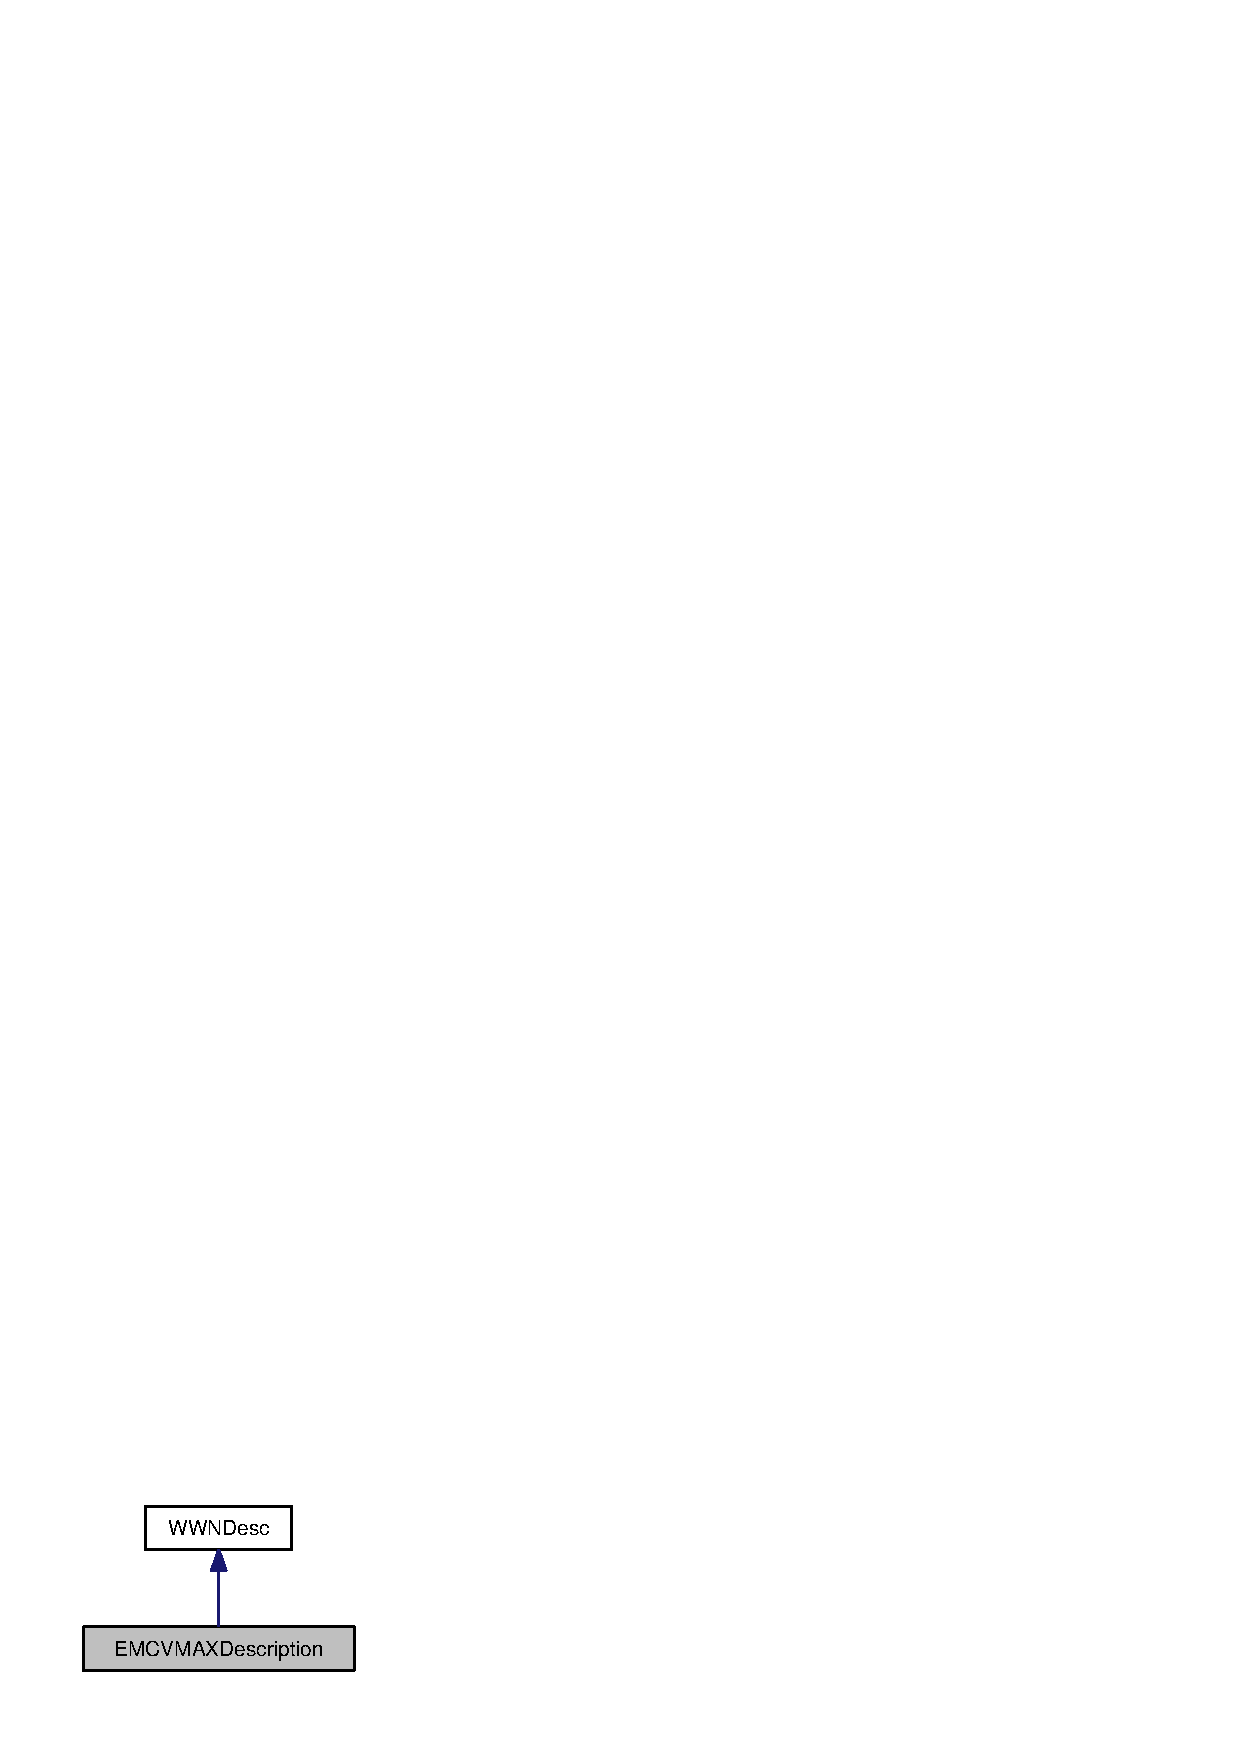
\includegraphics[width=174pt]{classorg_1_1smallfoot_1_1wwn_1_1EMCVMAXDescription__inherit__graph}
\end{center}
\end{figure}


Collaboration diagram for E\-M\-C\-V\-M\-A\-X\-Description\-:\nopagebreak
\begin{figure}[H]
\begin{center}
\leavevmode
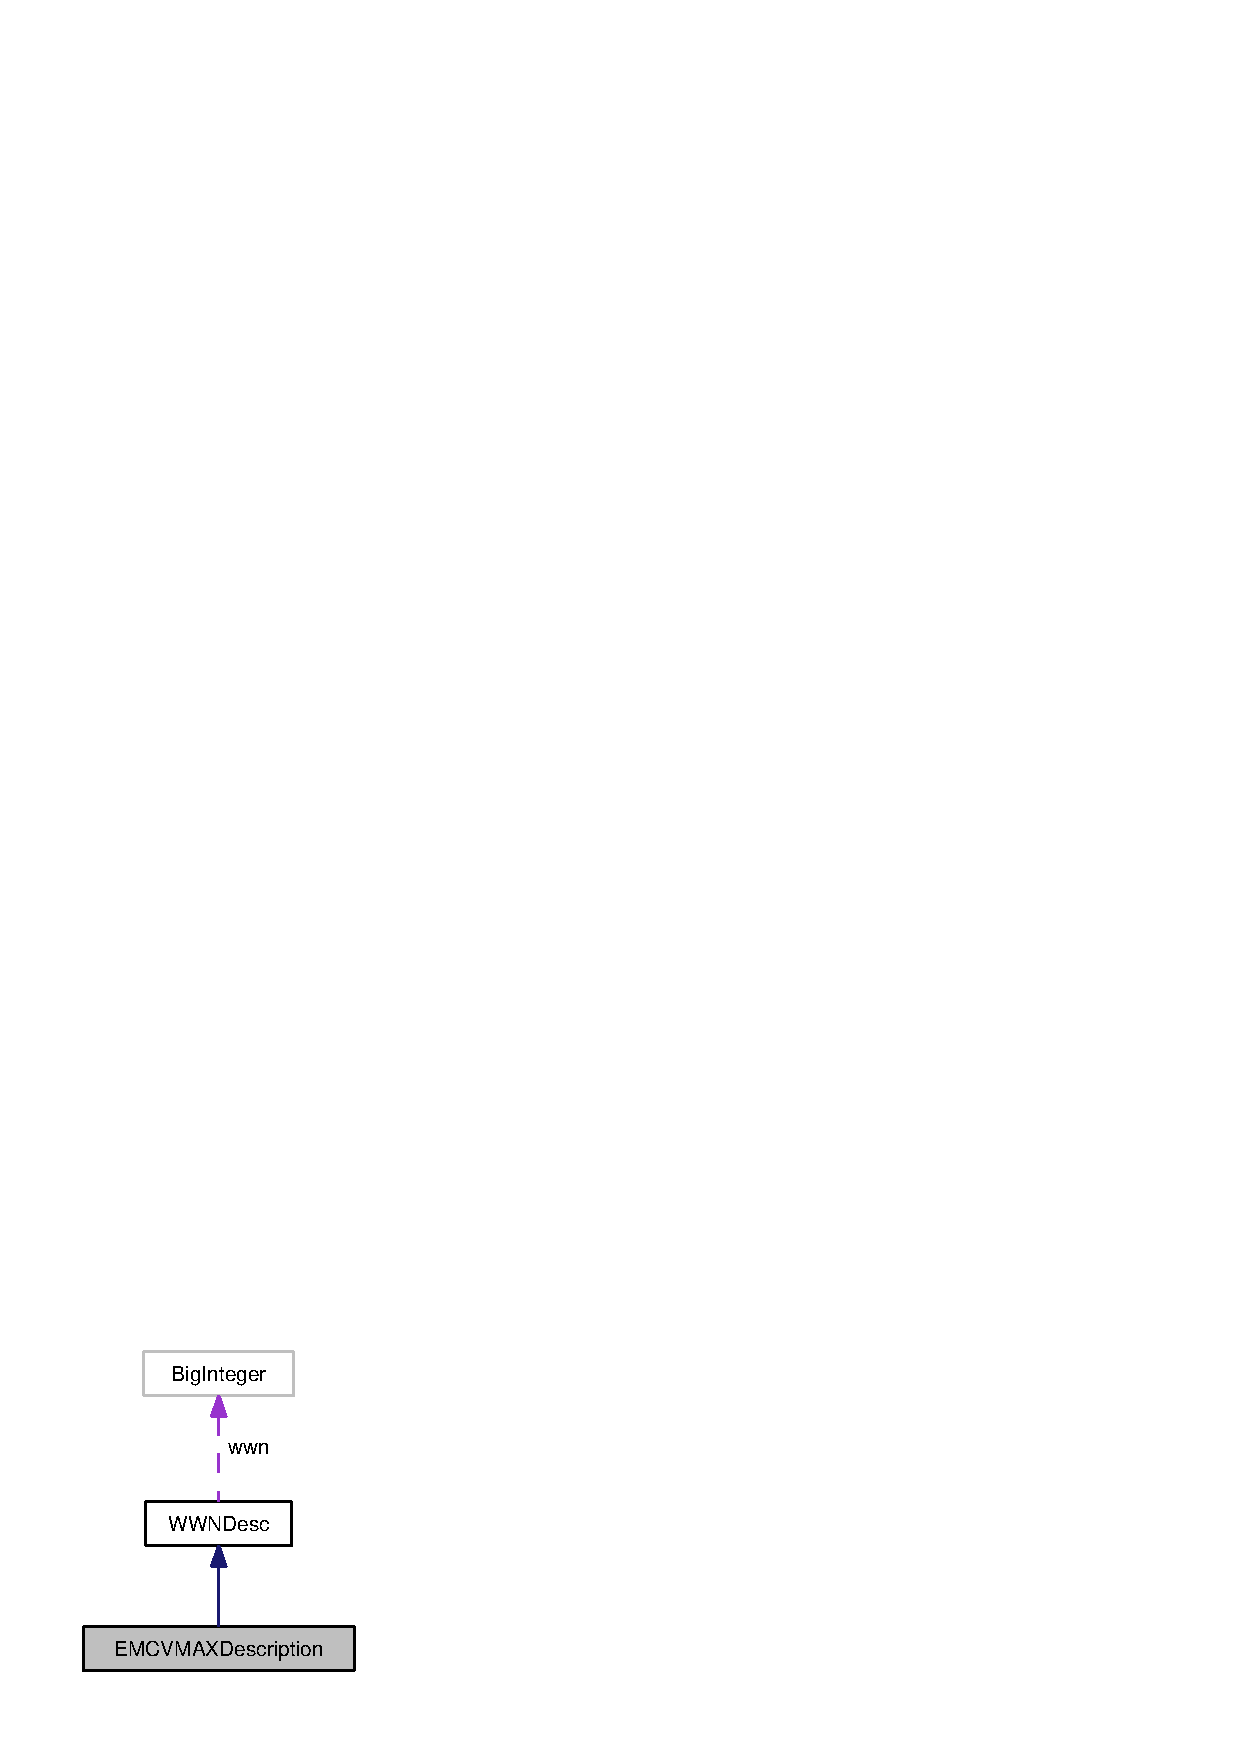
\includegraphics[width=174pt]{classorg_1_1smallfoot_1_1wwn_1_1EMCVMAXDescription__coll__graph}
\end{center}
\end{figure}
\subsection*{Public Member Functions}
\begin{DoxyCompactItemize}
\item 
{\bf E\-M\-C\-V\-M\-A\-X\-Description} (String {\bf wwn})
\begin{DoxyCompactList}\small\item\em create an instance with \doxyref{brief}{p.}{classorg_1_1smallfoot_1_1wwn_1_1WWNDesc_adbebed411e8c47d43338efa3edaa13f8} set to false. \end{DoxyCompactList}\item 
{\bf E\-M\-C\-V\-M\-A\-X\-Description} (boolean {\bf brief}, String {\bf wwn})
\begin{DoxyCompactList}\small\item\em create an instance with the given W\-W\-N. \end{DoxyCompactList}\item 
String {\bf to\-String} ()
\begin{DoxyCompactList}\small\item\em return a description or alias for this W\-W\-N; if brief is set to true during the call to \doxyref{get\-Desc()}{p.}{classorg_1_1smallfoot_1_1wwn_1_1EMCVMAXDescription_a7e34be4d9bd11a9971c007c6231b8c01}, then a shorter description or alias will be returned \end{DoxyCompactList}\end{DoxyCompactItemize}
\subsection*{Static Public Member Functions}
\begin{DoxyCompactItemize}
\item 
static {\bf W\-W\-N\-Desc} {\bf get\-Desc} (boolean strong, boolean {\bf brief}, String {\bf wwn})
\begin{DoxyCompactList}\small\item\em If this class matches or describes the given W\-W\-N, returns a new instance of this class loaded with the given W\-W\-N. \end{DoxyCompactList}\end{DoxyCompactItemize}
\subsection*{Additional Inherited Members}


\subsection{Detailed Description}
\doxyref{E\-M\-C\-V\-M\-A\-X\-Description}{p.}{classorg_1_1smallfoot_1_1wwn_1_1EMCVMAXDescription} (ie V\-Max-\/\-H\-K192601234-\/12g\-B or V\-Max-\/1234-\/12g\-B) breaks out the country of manufacturer, serial and F\-A port from the W\-W\-P\-N. 

\begin{DoxySeeAlso}{See Also}
\doxyref{E\-M\-C\-Clariion\-Description}{p.}{classorg_1_1smallfoot_1_1wwn_1_1EMCClariionDescription} 

\doxyref{E\-M\-C\-Symmetrix\-Description}{p.}{classorg_1_1smallfoot_1_1wwn_1_1EMCSymmetrixDescription} 

\doxyref{E\-M\-C\-V\-P\-L\-E\-X\-Description}{p.}{classorg_1_1smallfoot_1_1wwn_1_1EMCVPLEXDescription} 
\end{DoxySeeAlso}


Definition at line 13 of file E\-M\-C\-V\-M\-A\-X\-Description.\-java.



\subsection{Constructor \& Destructor Documentation}
\index{org\-::smallfoot\-::wwn\-::\-E\-M\-C\-V\-M\-A\-X\-Description@{org\-::smallfoot\-::wwn\-::\-E\-M\-C\-V\-M\-A\-X\-Description}!E\-M\-C\-V\-M\-A\-X\-Description@{E\-M\-C\-V\-M\-A\-X\-Description}}
\index{E\-M\-C\-V\-M\-A\-X\-Description@{E\-M\-C\-V\-M\-A\-X\-Description}!org::smallfoot::wwn::EMCVMAXDescription@{org\-::smallfoot\-::wwn\-::\-E\-M\-C\-V\-M\-A\-X\-Description}}
\subsubsection[{E\-M\-C\-V\-M\-A\-X\-Description}]{\setlength{\rightskip}{0pt plus 5cm}{\bf E\-M\-C\-V\-M\-A\-X\-Description} (
\begin{DoxyParamCaption}
\item[{String}]{wwn}
\end{DoxyParamCaption}
)\hspace{0.3cm}{\ttfamily [inline]}}\label{classorg_1_1smallfoot_1_1wwn_1_1EMCVMAXDescription_ad764133658fc6c5afec948ebd1873bb0}


create an instance with \doxyref{brief}{p.}{classorg_1_1smallfoot_1_1wwn_1_1WWNDesc_adbebed411e8c47d43338efa3edaa13f8} set to false. 

This is a convenience function to support the older constructor model


\begin{DoxyExceptions}{Exceptions}
{\em java.\-lang.\-Null\-Pointer\-Exception} & if the given wwn is null\\
\hline
\end{DoxyExceptions}

\begin{DoxyParams}{Parameters}
{\em wwn} & the W\-W\-N to evaluate and describe \\
\hline
\end{DoxyParams}


Definition at line 16 of file E\-M\-C\-V\-M\-A\-X\-Description.\-java.



Referenced by E\-M\-C\-V\-M\-A\-X\-Description.\-get\-Desc().

\index{org\-::smallfoot\-::wwn\-::\-E\-M\-C\-V\-M\-A\-X\-Description@{org\-::smallfoot\-::wwn\-::\-E\-M\-C\-V\-M\-A\-X\-Description}!E\-M\-C\-V\-M\-A\-X\-Description@{E\-M\-C\-V\-M\-A\-X\-Description}}
\index{E\-M\-C\-V\-M\-A\-X\-Description@{E\-M\-C\-V\-M\-A\-X\-Description}!org::smallfoot::wwn::EMCVMAXDescription@{org\-::smallfoot\-::wwn\-::\-E\-M\-C\-V\-M\-A\-X\-Description}}
\subsubsection[{E\-M\-C\-V\-M\-A\-X\-Description}]{\setlength{\rightskip}{0pt plus 5cm}{\bf E\-M\-C\-V\-M\-A\-X\-Description} (
\begin{DoxyParamCaption}
\item[{boolean}]{brief, }
\item[{String}]{wwn}
\end{DoxyParamCaption}
)\hspace{0.3cm}{\ttfamily [inline]}}\label{classorg_1_1smallfoot_1_1wwn_1_1EMCVMAXDescription_a348ba3a7bc4a038e1ff8479ac5d43a37}


create an instance with the given W\-W\-N. 

Values given to the constructor are simply copied to internal variables for later use


\begin{DoxyExceptions}{Exceptions}
{\em java.\-lang.\-Null\-Pointer\-Exception} & if the given wwn is null\\
\hline
\end{DoxyExceptions}

\begin{DoxyParams}{Parameters}
{\em brief} & whether an abbreviated description is requested \\
\hline
{\em wwn} & the W\-W\-N to evaluate and describe \\
\hline
\end{DoxyParams}


Definition at line 21 of file E\-M\-C\-V\-M\-A\-X\-Description.\-java.



\subsection{Member Function Documentation}
\index{org\-::smallfoot\-::wwn\-::\-E\-M\-C\-V\-M\-A\-X\-Description@{org\-::smallfoot\-::wwn\-::\-E\-M\-C\-V\-M\-A\-X\-Description}!get\-Desc@{get\-Desc}}
\index{get\-Desc@{get\-Desc}!org::smallfoot::wwn::EMCVMAXDescription@{org\-::smallfoot\-::wwn\-::\-E\-M\-C\-V\-M\-A\-X\-Description}}
\subsubsection[{get\-Desc}]{\setlength{\rightskip}{0pt plus 5cm}static {\bf W\-W\-N\-Desc} get\-Desc (
\begin{DoxyParamCaption}
\item[{boolean}]{strong, }
\item[{boolean}]{brief, }
\item[{String}]{wwn}
\end{DoxyParamCaption}
)\hspace{0.3cm}{\ttfamily [inline]}, {\ttfamily [static]}}\label{classorg_1_1smallfoot_1_1wwn_1_1EMCVMAXDescription_a7e34be4d9bd11a9971c007c6231b8c01}


If this class matches or describes the given W\-W\-N, returns a new instance of this class loaded with the given W\-W\-N. 

\begin{DoxyReturn}{Returns}
new instance of this class, or null if the given wwn does not match this class 
\end{DoxyReturn}

\begin{DoxyParams}{Parameters}
{\em strong} & is ignored\-: this class is a strong representation, not a weak one based on empirical matching, hence can always be used with confidence \\
\hline
{\em brief} & is used to ask for a shorter description\-: a more concise nickname or alias \\
\hline
{\em wwn} & the W\-W\-N (W\-W\-P\-N or W\-W\-N\-N, but typically W\-W\-P\-N) to match \\
\hline
\end{DoxyParams}


Definition at line 34 of file E\-M\-C\-V\-M\-A\-X\-Description.\-java.



References E\-M\-C\-V\-M\-A\-X\-Description.\-E\-M\-C\-V\-M\-A\-X\-Description().



Referenced by W\-W\-N\-Description.\-get\-W\-W\-N\-Descriptor().



Here is the call graph for this function\-:\nopagebreak
\begin{figure}[H]
\begin{center}
\leavevmode
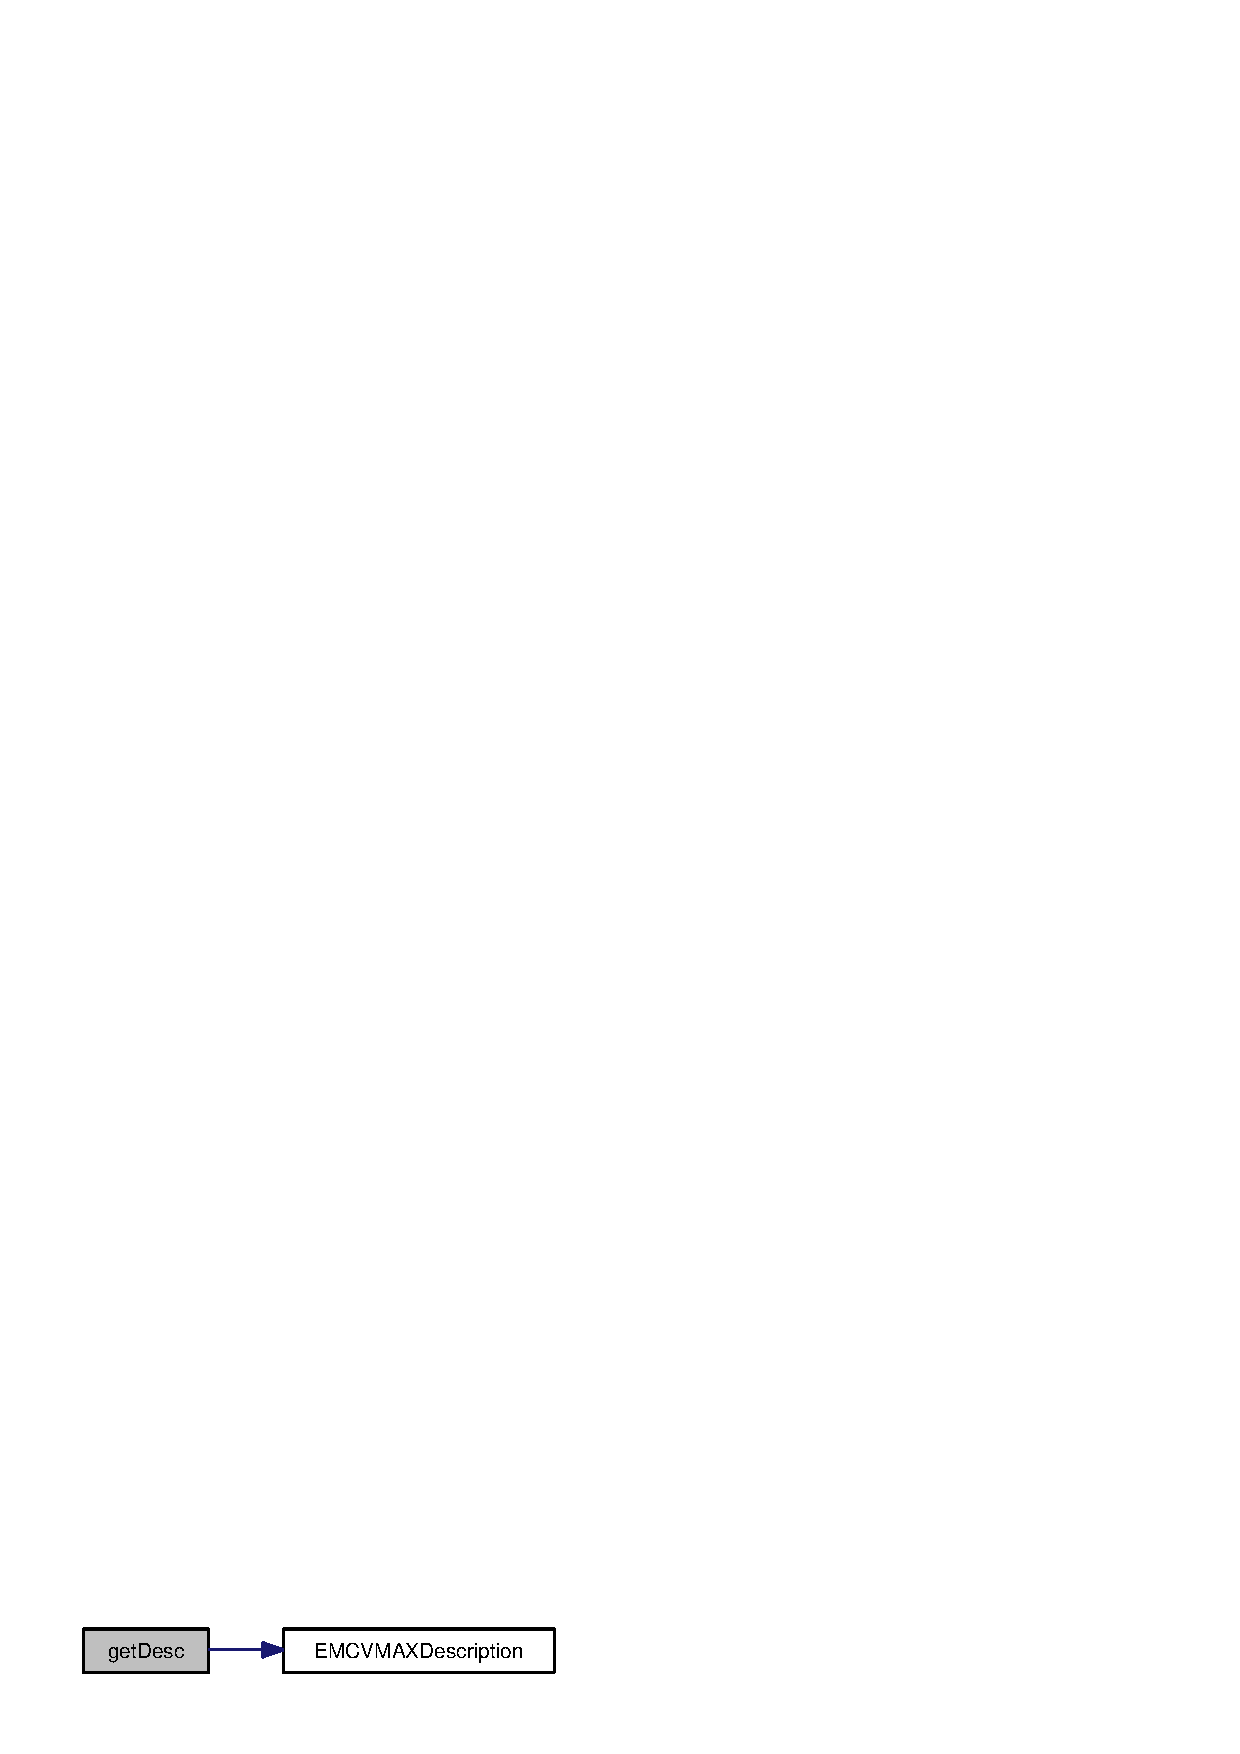
\includegraphics[width=270pt]{classorg_1_1smallfoot_1_1wwn_1_1EMCVMAXDescription_a7e34be4d9bd11a9971c007c6231b8c01_cgraph}
\end{center}
\end{figure}


\index{org\-::smallfoot\-::wwn\-::\-E\-M\-C\-V\-M\-A\-X\-Description@{org\-::smallfoot\-::wwn\-::\-E\-M\-C\-V\-M\-A\-X\-Description}!to\-String@{to\-String}}
\index{to\-String@{to\-String}!org::smallfoot::wwn::EMCVMAXDescription@{org\-::smallfoot\-::wwn\-::\-E\-M\-C\-V\-M\-A\-X\-Description}}
\subsubsection[{to\-String}]{\setlength{\rightskip}{0pt plus 5cm}String to\-String (
\begin{DoxyParamCaption}
{}
\end{DoxyParamCaption}
)\hspace{0.3cm}{\ttfamily [inline]}}\label{classorg_1_1smallfoot_1_1wwn_1_1EMCVMAXDescription_ad146fa8579a5f8a876c4688cc5a68520}


return a description or alias for this W\-W\-N; if brief is set to true during the call to \doxyref{get\-Desc()}{p.}{classorg_1_1smallfoot_1_1wwn_1_1EMCVMAXDescription_a7e34be4d9bd11a9971c007c6231b8c01}, then a shorter description or alias will be returned 

\begin{DoxySeeAlso}{See Also}
\doxyref{get\-Desc(boolean,boolean,\-String)}{p.}{classorg_1_1smallfoot_1_1wwn_1_1EMCVMAXDescription_a7e34be4d9bd11a9971c007c6231b8c01}
\end{DoxySeeAlso}
\begin{DoxyReturn}{Returns}
generated alias or nickname for the W\-W\-N 
\end{DoxyReturn}


Definition at line 49 of file E\-M\-C\-V\-M\-A\-X\-Description.\-java.



References W\-W\-N\-Desc.\-brief.



The documentation for this class was generated from the following file\-:\begin{DoxyCompactItemize}
\item 
java/{\bf E\-M\-C\-V\-M\-A\-X\-Description.\-java}\end{DoxyCompactItemize}

\section{E\-M\-C\-V\-P\-L\-E\-X\-Description Class Reference}
\label{classorg_1_1smallfoot_1_1wwn_1_1EMCVPLEXDescription}\index{E\-M\-C\-V\-P\-L\-E\-X\-Description@{E\-M\-C\-V\-P\-L\-E\-X\-Description}}


Inheritance diagram for E\-M\-C\-V\-P\-L\-E\-X\-Description\-:\nopagebreak
\begin{figure}[H]
\begin{center}
\leavevmode
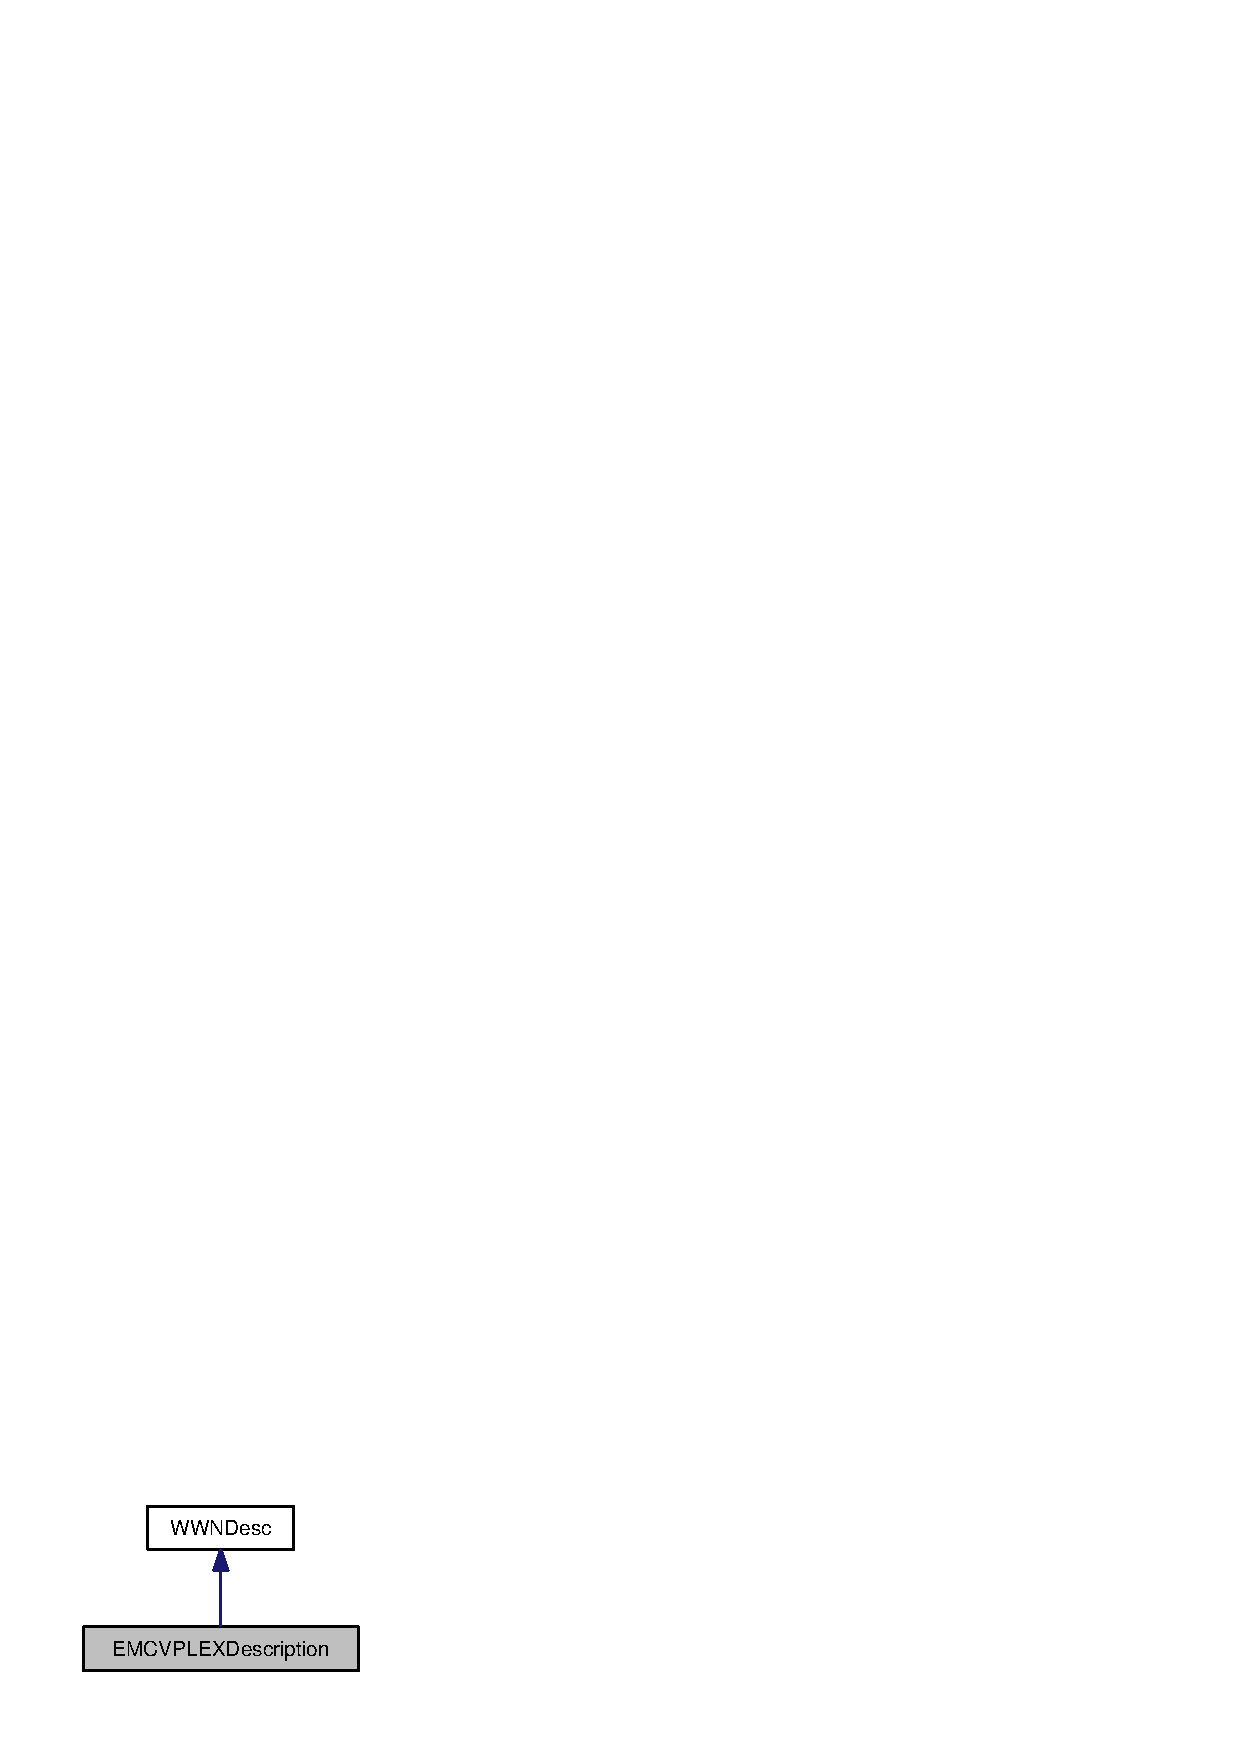
\includegraphics[width=176pt]{classorg_1_1smallfoot_1_1wwn_1_1EMCVPLEXDescription__inherit__graph}
\end{center}
\end{figure}


Collaboration diagram for E\-M\-C\-V\-P\-L\-E\-X\-Description\-:\nopagebreak
\begin{figure}[H]
\begin{center}
\leavevmode
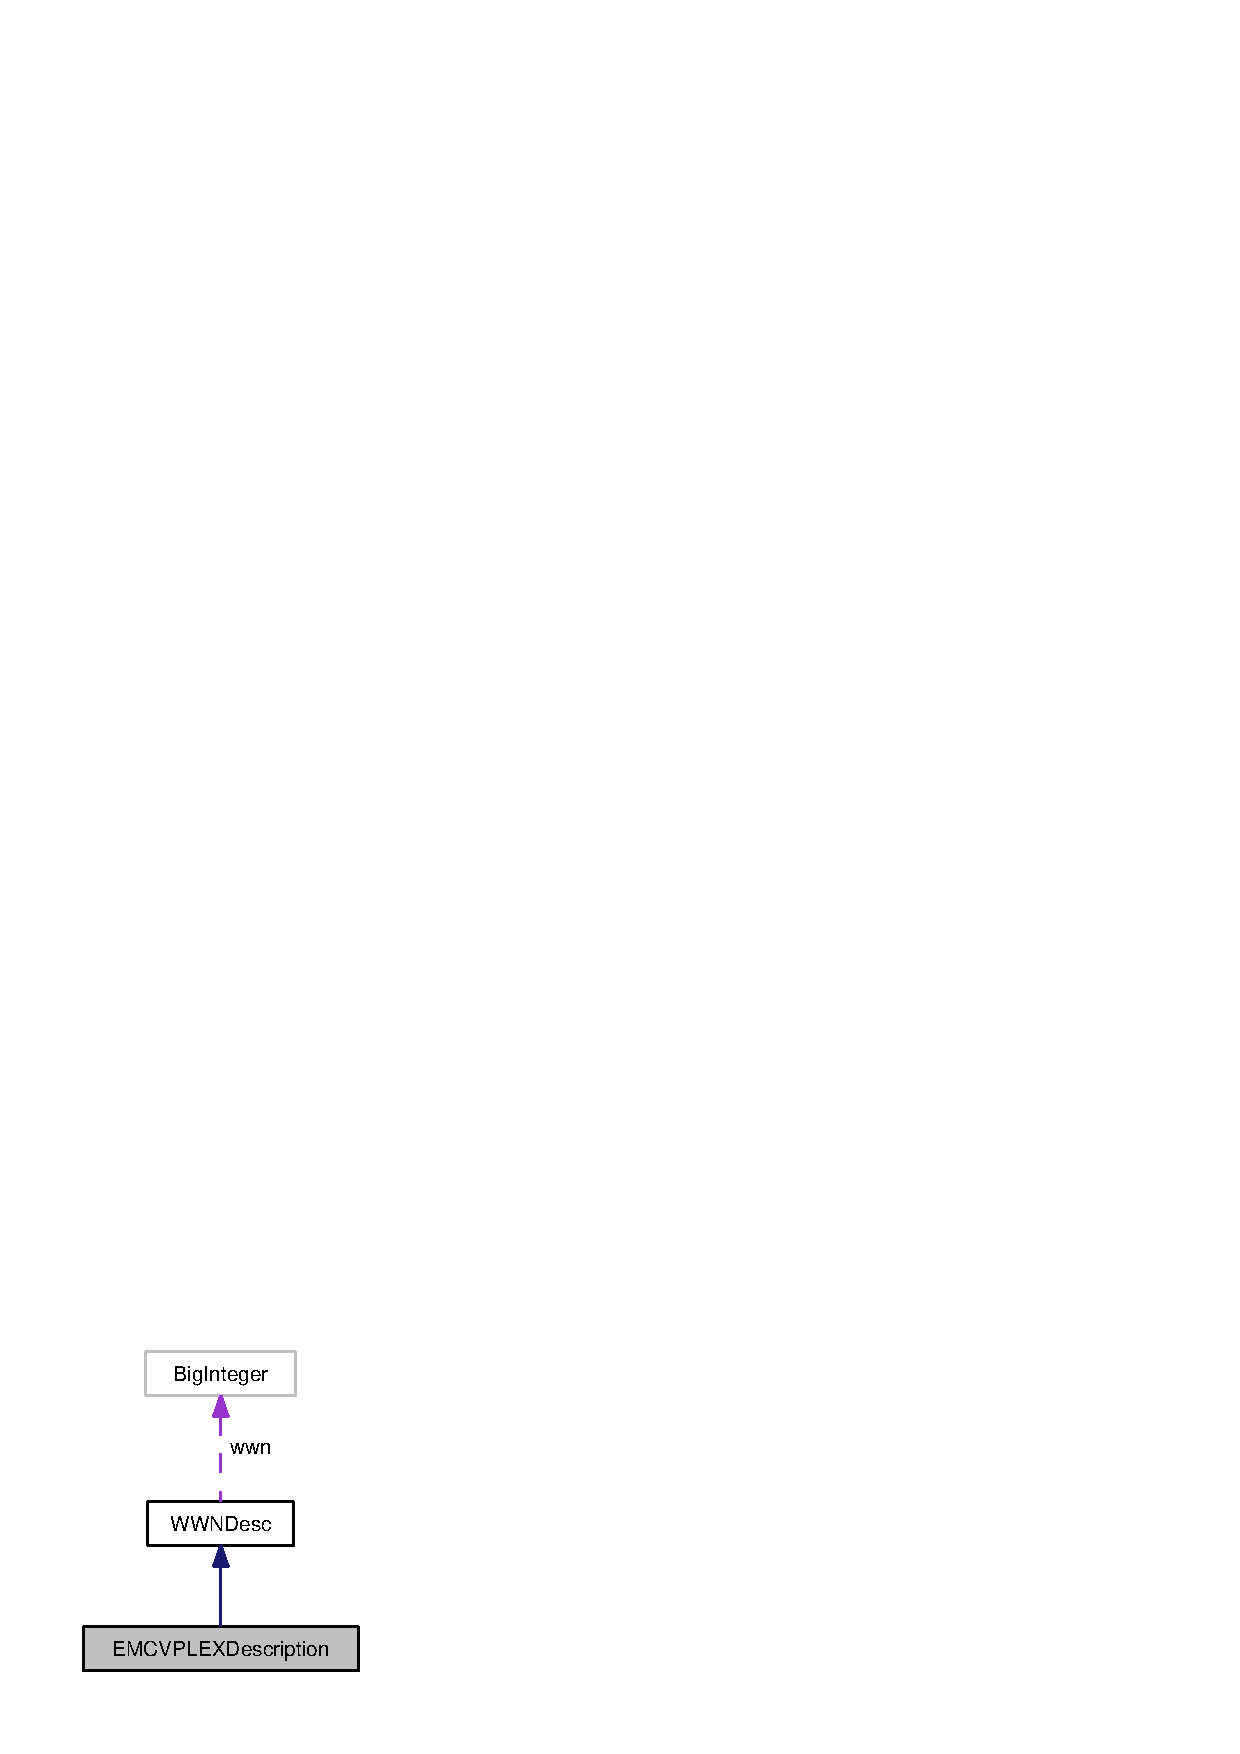
\includegraphics[width=176pt]{classorg_1_1smallfoot_1_1wwn_1_1EMCVPLEXDescription__coll__graph}
\end{center}
\end{figure}
\subsection*{Public Member Functions}
\begin{DoxyCompactItemize}
\item 
{\bf E\-M\-C\-V\-P\-L\-E\-X\-Description} (String wwn)
\begin{DoxyCompactList}\small\item\em create an instance with this.\-brief set to false. \end{DoxyCompactList}\item 
{\bf E\-M\-C\-V\-P\-L\-E\-X\-Description} (boolean brief, String wwn)
\begin{DoxyCompactList}\small\item\em create an instance with the given W\-W\-N. \end{DoxyCompactList}\item 
String {\bf to\-String} ()
\begin{DoxyCompactList}\small\item\em return a description or alias for this W\-W\-N; if brief is set to true during the call to \doxyref{get\-Desc()}{p.}{classorg_1_1smallfoot_1_1wwn_1_1EMCVPLEXDescription_a7e34be4d9bd11a9971c007c6231b8c01}, then a shorter description or alias will be returned \end{DoxyCompactList}\end{DoxyCompactItemize}
\subsection*{Static Public Member Functions}
\begin{DoxyCompactItemize}
\item 
static {\bf W\-W\-N\-Desc} {\bf get\-Desc} (boolean strong, boolean brief, String wwn)
\begin{DoxyCompactList}\small\item\em If this class matches or describes the given W\-W\-N, returns a new instance of this class loaded with the given W\-W\-N. \end{DoxyCompactList}\end{DoxyCompactItemize}


\subsection{Detailed Description}


Definition at line 10 of file E\-M\-C\-V\-P\-L\-E\-X\-Description.\-java.



\subsection{Constructor \& Destructor Documentation}
\index{org\-::smallfoot\-::wwn\-::\-E\-M\-C\-V\-P\-L\-E\-X\-Description@{org\-::smallfoot\-::wwn\-::\-E\-M\-C\-V\-P\-L\-E\-X\-Description}!E\-M\-C\-V\-P\-L\-E\-X\-Description@{E\-M\-C\-V\-P\-L\-E\-X\-Description}}
\index{E\-M\-C\-V\-P\-L\-E\-X\-Description@{E\-M\-C\-V\-P\-L\-E\-X\-Description}!org::smallfoot::wwn::EMCVPLEXDescription@{org\-::smallfoot\-::wwn\-::\-E\-M\-C\-V\-P\-L\-E\-X\-Description}}
\subsubsection[{E\-M\-C\-V\-P\-L\-E\-X\-Description}]{\setlength{\rightskip}{0pt plus 5cm}{\bf E\-M\-C\-V\-P\-L\-E\-X\-Description} (
\begin{DoxyParamCaption}
\item[{String}]{wwn}
\end{DoxyParamCaption}
)\hspace{0.3cm}{\ttfamily [inline]}}\label{classorg_1_1smallfoot_1_1wwn_1_1EMCVPLEXDescription_a022d1e6232e295b14d9ec8c05a9472c7}


create an instance with this.\-brief set to false. 

This is a convenience function to support the older constructor model


\begin{DoxyParams}{Parameters}
{\em wwn} & the W\-W\-N to evaluate and describe \\
\hline
\end{DoxyParams}


Definition at line 13 of file E\-M\-C\-V\-P\-L\-E\-X\-Description.\-java.



Referenced by E\-M\-C\-V\-P\-L\-E\-X\-Description.\-get\-Desc().

\index{org\-::smallfoot\-::wwn\-::\-E\-M\-C\-V\-P\-L\-E\-X\-Description@{org\-::smallfoot\-::wwn\-::\-E\-M\-C\-V\-P\-L\-E\-X\-Description}!E\-M\-C\-V\-P\-L\-E\-X\-Description@{E\-M\-C\-V\-P\-L\-E\-X\-Description}}
\index{E\-M\-C\-V\-P\-L\-E\-X\-Description@{E\-M\-C\-V\-P\-L\-E\-X\-Description}!org::smallfoot::wwn::EMCVPLEXDescription@{org\-::smallfoot\-::wwn\-::\-E\-M\-C\-V\-P\-L\-E\-X\-Description}}
\subsubsection[{E\-M\-C\-V\-P\-L\-E\-X\-Description}]{\setlength{\rightskip}{0pt plus 5cm}{\bf E\-M\-C\-V\-P\-L\-E\-X\-Description} (
\begin{DoxyParamCaption}
\item[{boolean}]{brief, }
\item[{String}]{wwn}
\end{DoxyParamCaption}
)\hspace{0.3cm}{\ttfamily [inline]}}\label{classorg_1_1smallfoot_1_1wwn_1_1EMCVPLEXDescription_a6803024e3e1d731aa60b5f3b46903349}


create an instance with the given W\-W\-N. 

Values given to the constructor are simply copied to internal variables for later use


\begin{DoxyParams}{Parameters}
{\em brief} & whether an abbreviated description is requested \\
\hline
{\em wwn} & the W\-W\-N to evaluate and describe \\
\hline
\end{DoxyParams}


Definition at line 18 of file E\-M\-C\-V\-P\-L\-E\-X\-Description.\-java.



\subsection{Member Function Documentation}
\index{org\-::smallfoot\-::wwn\-::\-E\-M\-C\-V\-P\-L\-E\-X\-Description@{org\-::smallfoot\-::wwn\-::\-E\-M\-C\-V\-P\-L\-E\-X\-Description}!get\-Desc@{get\-Desc}}
\index{get\-Desc@{get\-Desc}!org::smallfoot::wwn::EMCVPLEXDescription@{org\-::smallfoot\-::wwn\-::\-E\-M\-C\-V\-P\-L\-E\-X\-Description}}
\subsubsection[{get\-Desc}]{\setlength{\rightskip}{0pt plus 5cm}static {\bf W\-W\-N\-Desc} get\-Desc (
\begin{DoxyParamCaption}
\item[{boolean}]{strong, }
\item[{boolean}]{brief, }
\item[{String}]{wwn}
\end{DoxyParamCaption}
)\hspace{0.3cm}{\ttfamily [inline]}, {\ttfamily [static]}}\label{classorg_1_1smallfoot_1_1wwn_1_1EMCVPLEXDescription_a7e34be4d9bd11a9971c007c6231b8c01}


If this class matches or describes the given W\-W\-N, returns a new instance of this class loaded with the given W\-W\-N. 

\begin{DoxyReturn}{Returns}
new instance of this class, or null if the given wwn does not match this class 
\end{DoxyReturn}

\begin{DoxyParams}{Parameters}
{\em strong} & is ignored\-: this class is a strong representation, not a weak one based on empirical matching, hence can always be used with confidence \\
\hline
{\em brief} & is used to ask for a shorter description\-: a more concise nickname or alias \\
\hline
{\em wwn} & the W\-W\-N (W\-W\-P\-N or W\-W\-N\-N, but typically W\-W\-P\-N) to match \\
\hline
\end{DoxyParams}


Definition at line 31 of file E\-M\-C\-V\-P\-L\-E\-X\-Description.\-java.



References E\-M\-C\-V\-P\-L\-E\-X\-Description.\-E\-M\-C\-V\-P\-L\-E\-X\-Description().



Referenced by W\-W\-N\-Description.\-get\-W\-W\-N\-Descriptor().



Here is the call graph for this function\-:\nopagebreak
\begin{figure}[H]
\begin{center}
\leavevmode
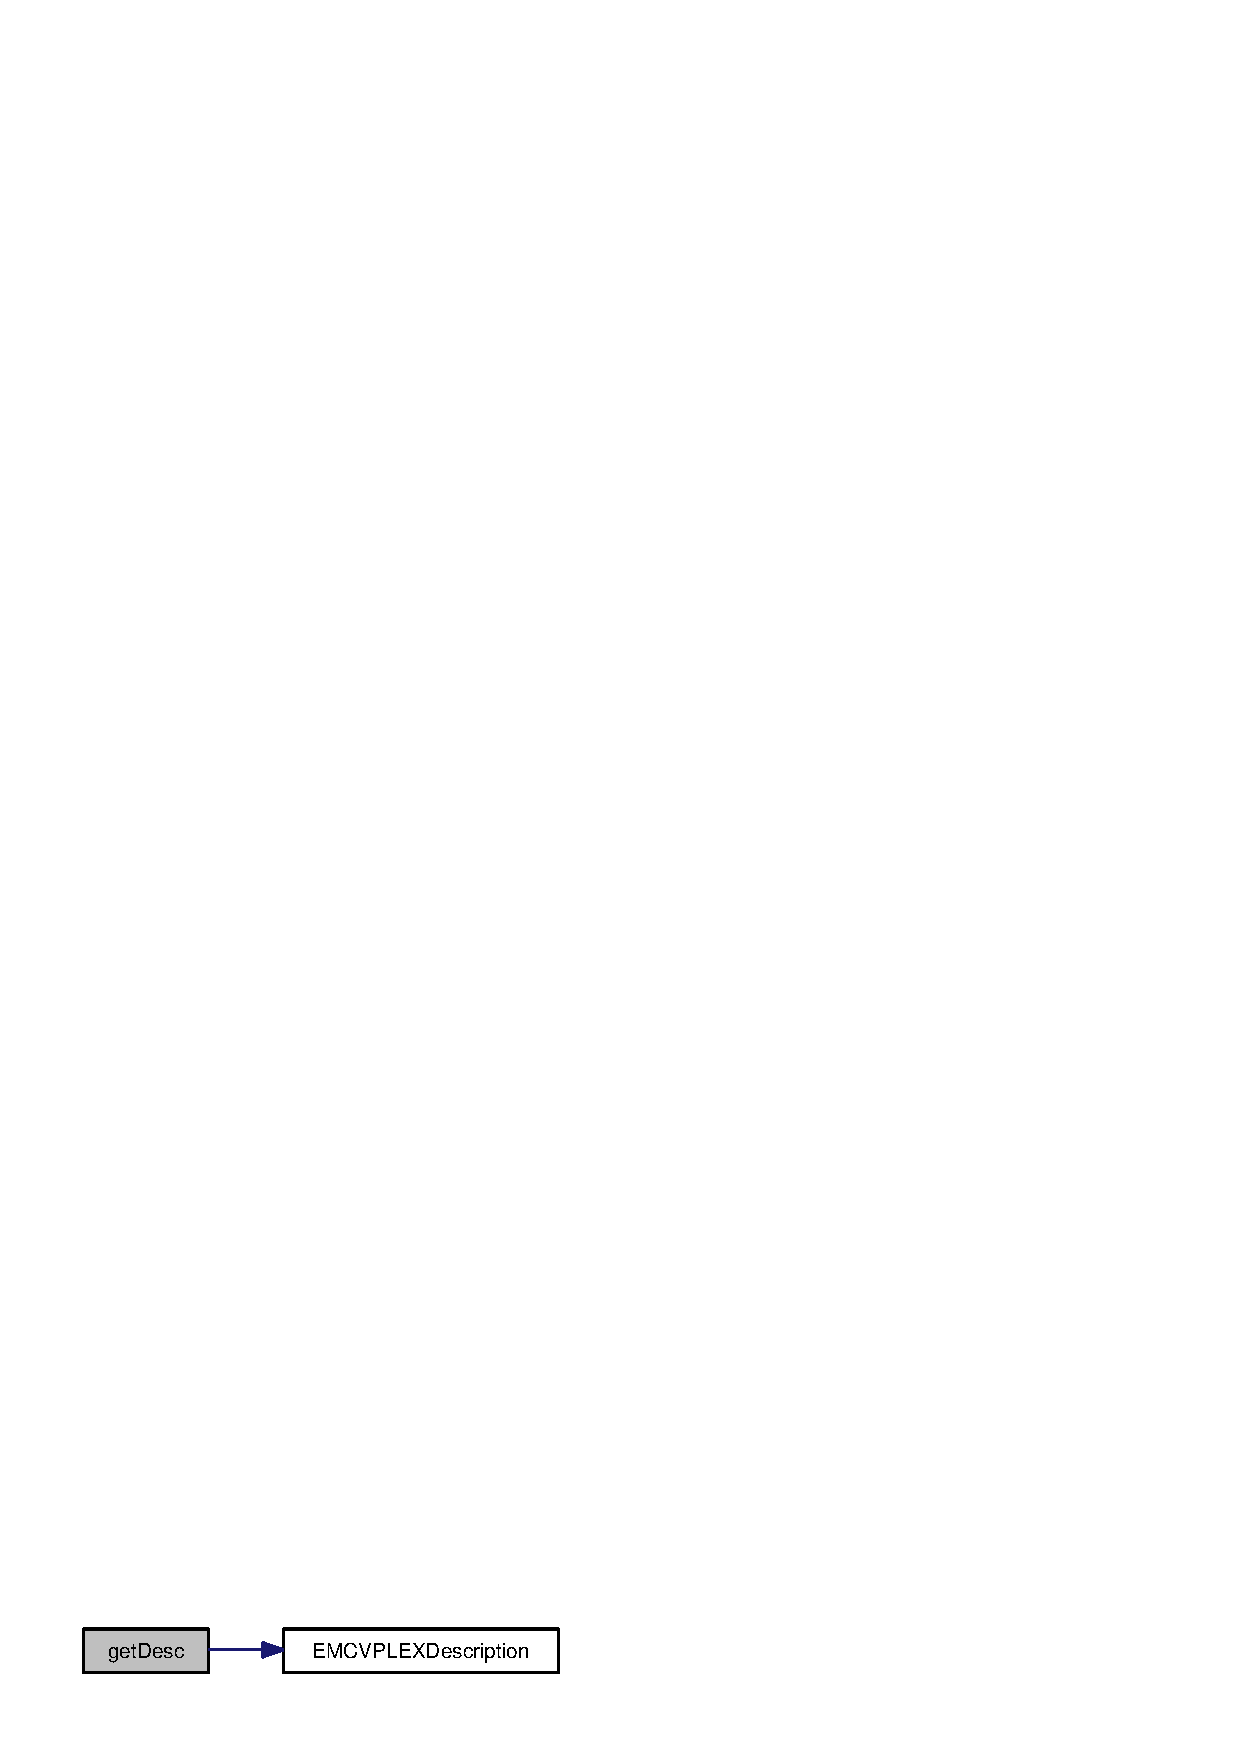
\includegraphics[width=272pt]{classorg_1_1smallfoot_1_1wwn_1_1EMCVPLEXDescription_a7e34be4d9bd11a9971c007c6231b8c01_cgraph}
\end{center}
\end{figure}


\index{org\-::smallfoot\-::wwn\-::\-E\-M\-C\-V\-P\-L\-E\-X\-Description@{org\-::smallfoot\-::wwn\-::\-E\-M\-C\-V\-P\-L\-E\-X\-Description}!to\-String@{to\-String}}
\index{to\-String@{to\-String}!org::smallfoot::wwn::EMCVPLEXDescription@{org\-::smallfoot\-::wwn\-::\-E\-M\-C\-V\-P\-L\-E\-X\-Description}}
\subsubsection[{to\-String}]{\setlength{\rightskip}{0pt plus 5cm}String to\-String (
\begin{DoxyParamCaption}
{}
\end{DoxyParamCaption}
)\hspace{0.3cm}{\ttfamily [inline]}}\label{classorg_1_1smallfoot_1_1wwn_1_1EMCVPLEXDescription_ad146fa8579a5f8a876c4688cc5a68520}


return a description or alias for this W\-W\-N; if brief is set to true during the call to \doxyref{get\-Desc()}{p.}{classorg_1_1smallfoot_1_1wwn_1_1EMCVPLEXDescription_a7e34be4d9bd11a9971c007c6231b8c01}, then a shorter description or alias will be returned 

\begin{DoxySeeAlso}{See Also}
\doxyref{get\-Desc(boolean,boolean,\-String)}{p.}{classorg_1_1smallfoot_1_1wwn_1_1EMCVPLEXDescription_a7e34be4d9bd11a9971c007c6231b8c01}
\end{DoxySeeAlso}
\begin{DoxyReturn}{Returns}
generated alias or nickname for the W\-W\-N 
\end{DoxyReturn}


Definition at line 46 of file E\-M\-C\-V\-P\-L\-E\-X\-Description.\-java.



The documentation for this class was generated from the following file\-:\begin{DoxyCompactItemize}
\item 
java/{\bf E\-M\-C\-V\-P\-L\-E\-X\-Description.\-java}\end{DoxyCompactItemize}

\section{H\-D\-S\-V\-S\-P\-Description Class Reference}
\label{classorg_1_1smallfoot_1_1wwn_1_1HDSVSPDescription}\index{H\-D\-S\-V\-S\-P\-Description@{H\-D\-S\-V\-S\-P\-Description}}


Inheritance diagram for H\-D\-S\-V\-S\-P\-Description\-:\nopagebreak
\begin{figure}[H]
\begin{center}
\leavevmode
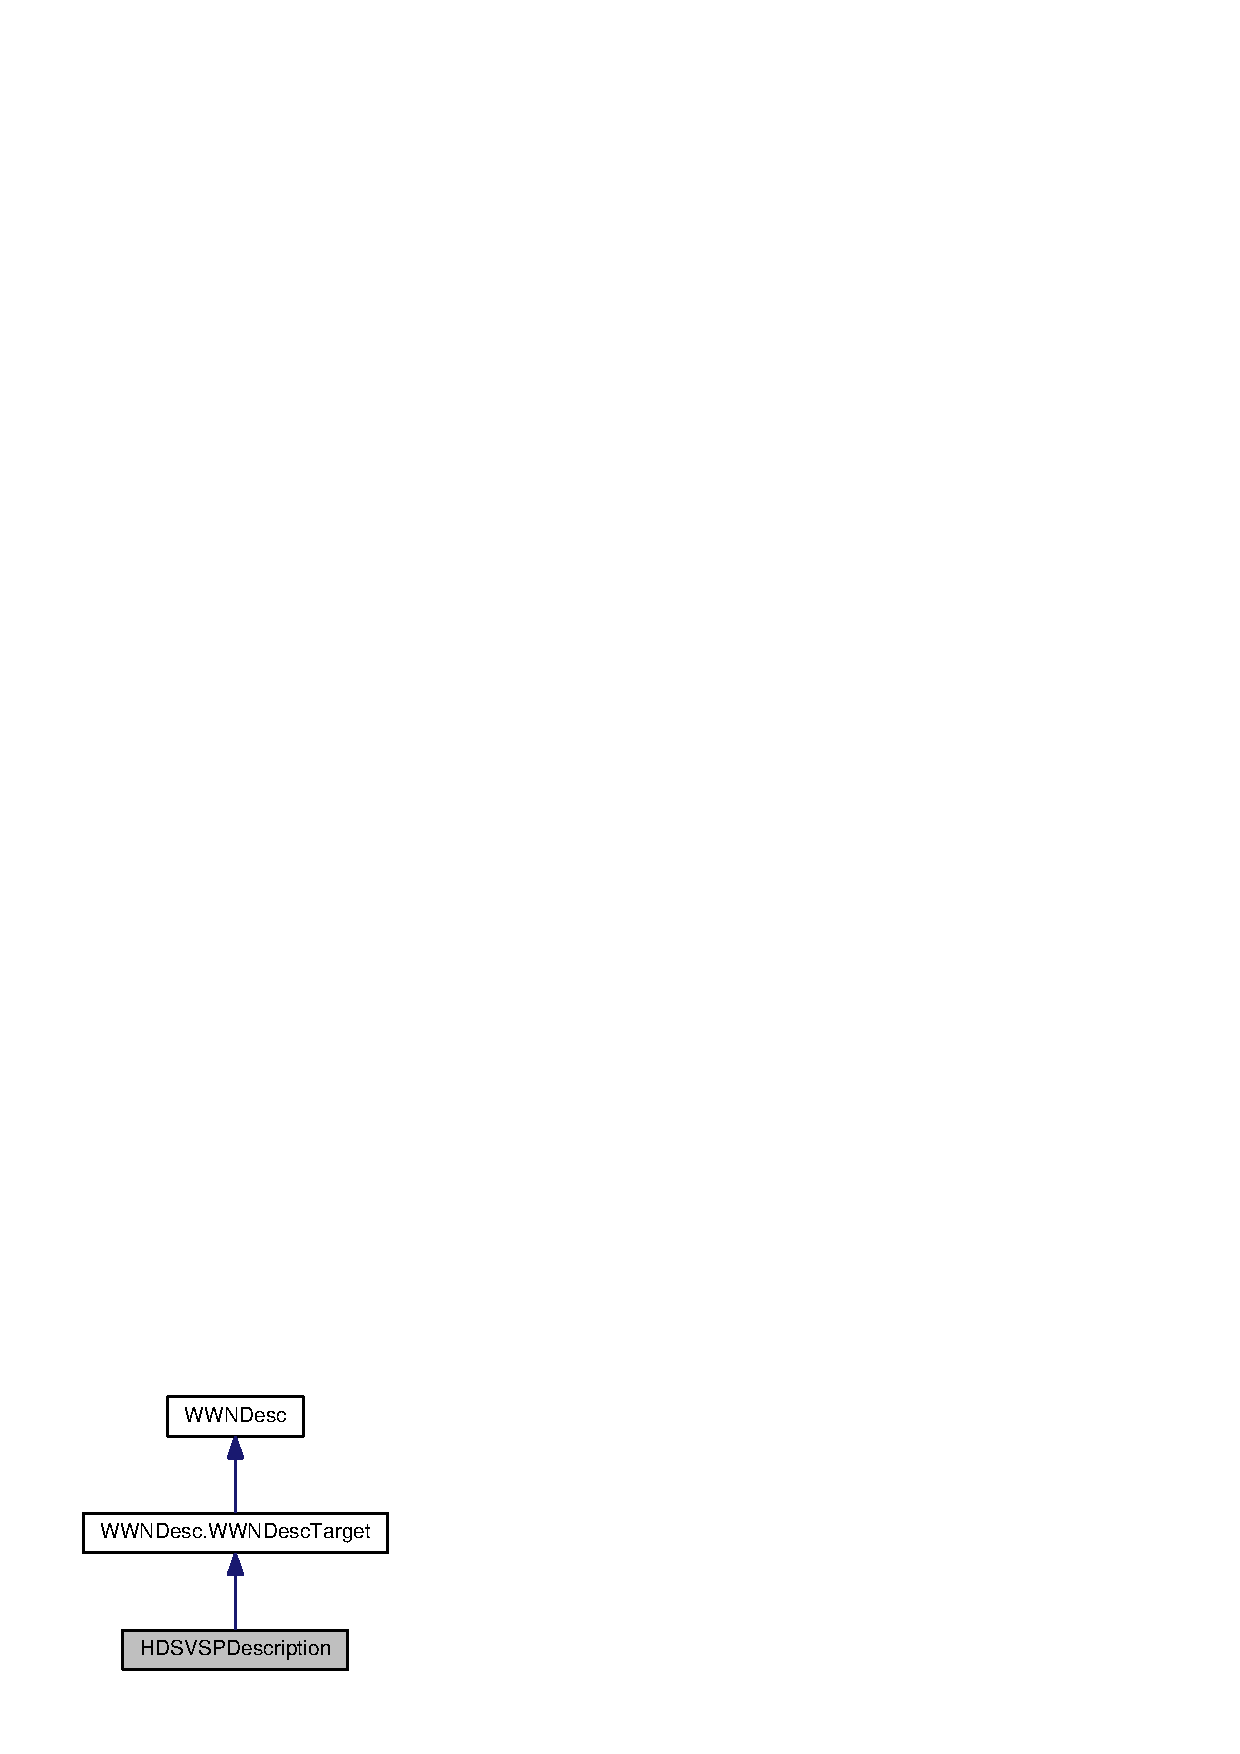
\includegraphics[width=164pt]{classorg_1_1smallfoot_1_1wwn_1_1HDSVSPDescription__inherit__graph}
\end{center}
\end{figure}


Collaboration diagram for H\-D\-S\-V\-S\-P\-Description\-:\nopagebreak
\begin{figure}[H]
\begin{center}
\leavevmode
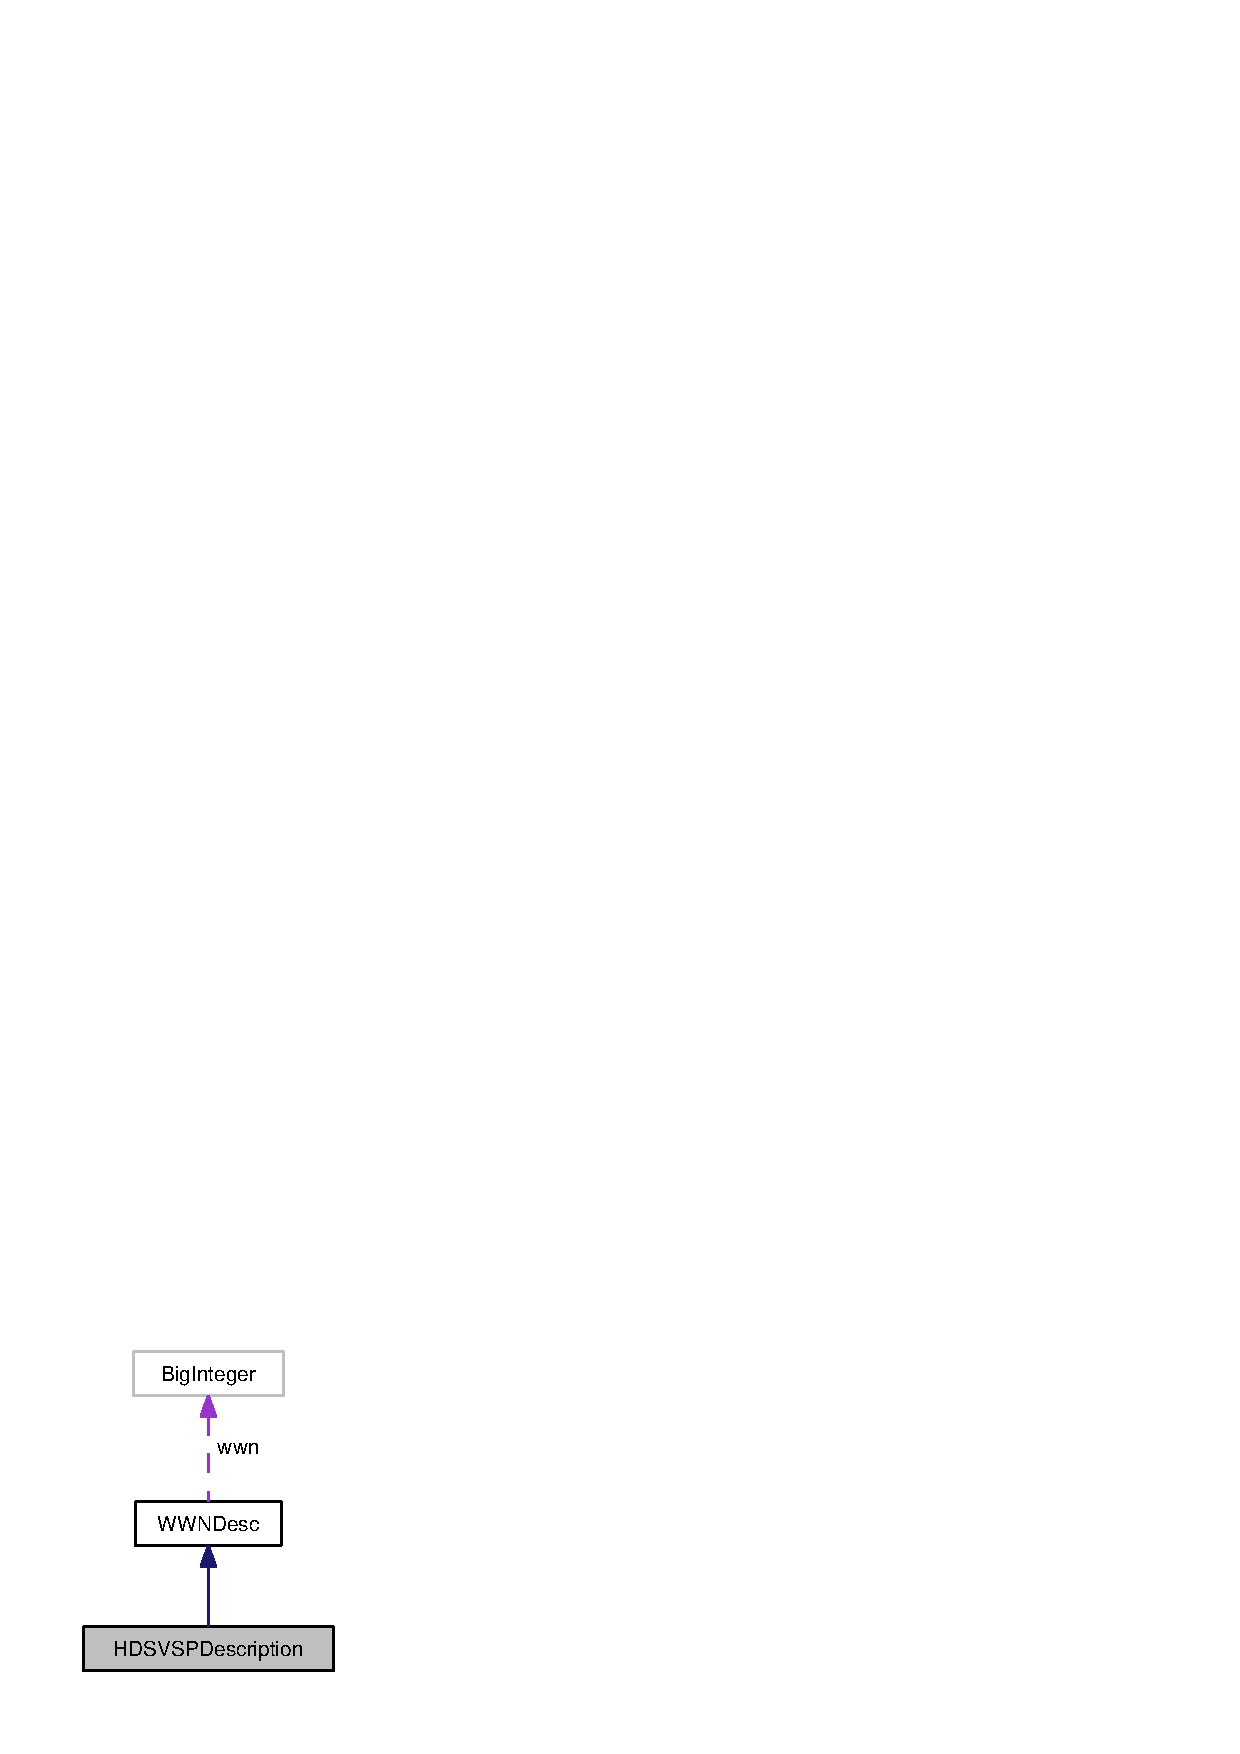
\includegraphics[width=164pt]{classorg_1_1smallfoot_1_1wwn_1_1HDSVSPDescription__coll__graph}
\end{center}
\end{figure}
\subsection*{Public Member Functions}
\begin{DoxyCompactItemize}
\item 
{\bf H\-D\-S\-V\-S\-P\-Description} (String wwn)
\begin{DoxyCompactList}\small\item\em create an instance with this.\-brief set to false. \end{DoxyCompactList}\item 
{\bf H\-D\-S\-V\-S\-P\-Description} (boolean brief, String wwn)
\begin{DoxyCompactList}\small\item\em create an instance with the given W\-W\-N. \end{DoxyCompactList}\item 
String {\bf to\-String} ()
\begin{DoxyCompactList}\small\item\em return a description or alias for this W\-W\-N; if brief is set to true during the call to \doxyref{get\-Desc()}{p.}{classorg_1_1smallfoot_1_1wwn_1_1HDSVSPDescription_a7e34be4d9bd11a9971c007c6231b8c01}, then a shorter description or alias will be returned \end{DoxyCompactList}\end{DoxyCompactItemize}
\subsection*{Static Public Member Functions}
\begin{DoxyCompactItemize}
\item 
static {\bf W\-W\-N\-Desc} {\bf get\-Desc} (boolean strong, boolean brief, String wwn)
\begin{DoxyCompactList}\small\item\em If this class matches or describes the given W\-W\-N, returns a new instance of this class loaded with the given W\-W\-N. \end{DoxyCompactList}\end{DoxyCompactItemize}


\subsection{Detailed Description}


Definition at line 10 of file H\-D\-S\-V\-S\-P\-Description.\-java.



\subsection{Constructor \& Destructor Documentation}
\index{org\-::smallfoot\-::wwn\-::\-H\-D\-S\-V\-S\-P\-Description@{org\-::smallfoot\-::wwn\-::\-H\-D\-S\-V\-S\-P\-Description}!H\-D\-S\-V\-S\-P\-Description@{H\-D\-S\-V\-S\-P\-Description}}
\index{H\-D\-S\-V\-S\-P\-Description@{H\-D\-S\-V\-S\-P\-Description}!org::smallfoot::wwn::HDSVSPDescription@{org\-::smallfoot\-::wwn\-::\-H\-D\-S\-V\-S\-P\-Description}}
\subsubsection[{H\-D\-S\-V\-S\-P\-Description}]{\setlength{\rightskip}{0pt plus 5cm}{\bf H\-D\-S\-V\-S\-P\-Description} (
\begin{DoxyParamCaption}
\item[{String}]{wwn}
\end{DoxyParamCaption}
)\hspace{0.3cm}{\ttfamily [inline]}}\label{classorg_1_1smallfoot_1_1wwn_1_1HDSVSPDescription_a3c873624b4dd44f373af3dc3e445f02c}


create an instance with this.\-brief set to false. 

This is a convenience function to support the older constructor model


\begin{DoxyParams}{Parameters}
{\em wwn} & the W\-W\-N to evaluate and describe \\
\hline
\end{DoxyParams}


Definition at line 13 of file H\-D\-S\-V\-S\-P\-Description.\-java.



Referenced by H\-D\-S\-V\-S\-P\-Description.\-get\-Desc().

\index{org\-::smallfoot\-::wwn\-::\-H\-D\-S\-V\-S\-P\-Description@{org\-::smallfoot\-::wwn\-::\-H\-D\-S\-V\-S\-P\-Description}!H\-D\-S\-V\-S\-P\-Description@{H\-D\-S\-V\-S\-P\-Description}}
\index{H\-D\-S\-V\-S\-P\-Description@{H\-D\-S\-V\-S\-P\-Description}!org::smallfoot::wwn::HDSVSPDescription@{org\-::smallfoot\-::wwn\-::\-H\-D\-S\-V\-S\-P\-Description}}
\subsubsection[{H\-D\-S\-V\-S\-P\-Description}]{\setlength{\rightskip}{0pt plus 5cm}{\bf H\-D\-S\-V\-S\-P\-Description} (
\begin{DoxyParamCaption}
\item[{boolean}]{brief, }
\item[{String}]{wwn}
\end{DoxyParamCaption}
)\hspace{0.3cm}{\ttfamily [inline]}}\label{classorg_1_1smallfoot_1_1wwn_1_1HDSVSPDescription_af2cd2d4fa950688e68f7bcda4b35e9d1}


create an instance with the given W\-W\-N. 

Values given to the constructor are simply copied to internal variables for later use


\begin{DoxyParams}{Parameters}
{\em brief} & whether an abbreviated description is requested \\
\hline
{\em wwn} & the W\-W\-N to evaluate and describe \\
\hline
\end{DoxyParams}


Definition at line 18 of file H\-D\-S\-V\-S\-P\-Description.\-java.



\subsection{Member Function Documentation}
\index{org\-::smallfoot\-::wwn\-::\-H\-D\-S\-V\-S\-P\-Description@{org\-::smallfoot\-::wwn\-::\-H\-D\-S\-V\-S\-P\-Description}!get\-Desc@{get\-Desc}}
\index{get\-Desc@{get\-Desc}!org::smallfoot::wwn::HDSVSPDescription@{org\-::smallfoot\-::wwn\-::\-H\-D\-S\-V\-S\-P\-Description}}
\subsubsection[{get\-Desc}]{\setlength{\rightskip}{0pt plus 5cm}static {\bf W\-W\-N\-Desc} get\-Desc (
\begin{DoxyParamCaption}
\item[{boolean}]{strong, }
\item[{boolean}]{brief, }
\item[{String}]{wwn}
\end{DoxyParamCaption}
)\hspace{0.3cm}{\ttfamily [inline]}, {\ttfamily [static]}}\label{classorg_1_1smallfoot_1_1wwn_1_1HDSVSPDescription_a7e34be4d9bd11a9971c007c6231b8c01}


If this class matches or describes the given W\-W\-N, returns a new instance of this class loaded with the given W\-W\-N. 

\begin{DoxyReturn}{Returns}
new instance of this class, or null if the given wwn does not match this class 
\end{DoxyReturn}

\begin{DoxyParams}{Parameters}
{\em strong} & is ignored\-: this class is a strong representation, not a weak one based on empirical matching, hence can always be used with confidence \\
\hline
{\em brief} & is used to ask for a shorter description\-: a more concise nickname or alias \\
\hline
{\em wwn} & the W\-W\-N (W\-W\-P\-N or W\-W\-N\-N, but typically W\-W\-P\-N) to match \\
\hline
\end{DoxyParams}


Definition at line 31 of file H\-D\-S\-V\-S\-P\-Description.\-java.



References H\-D\-S\-V\-S\-P\-Description.\-H\-D\-S\-V\-S\-P\-Description().



Referenced by W\-W\-N\-Description.\-get\-W\-W\-N\-Descriptor().



Here is the call graph for this function\-:\nopagebreak
\begin{figure}[H]
\begin{center}
\leavevmode
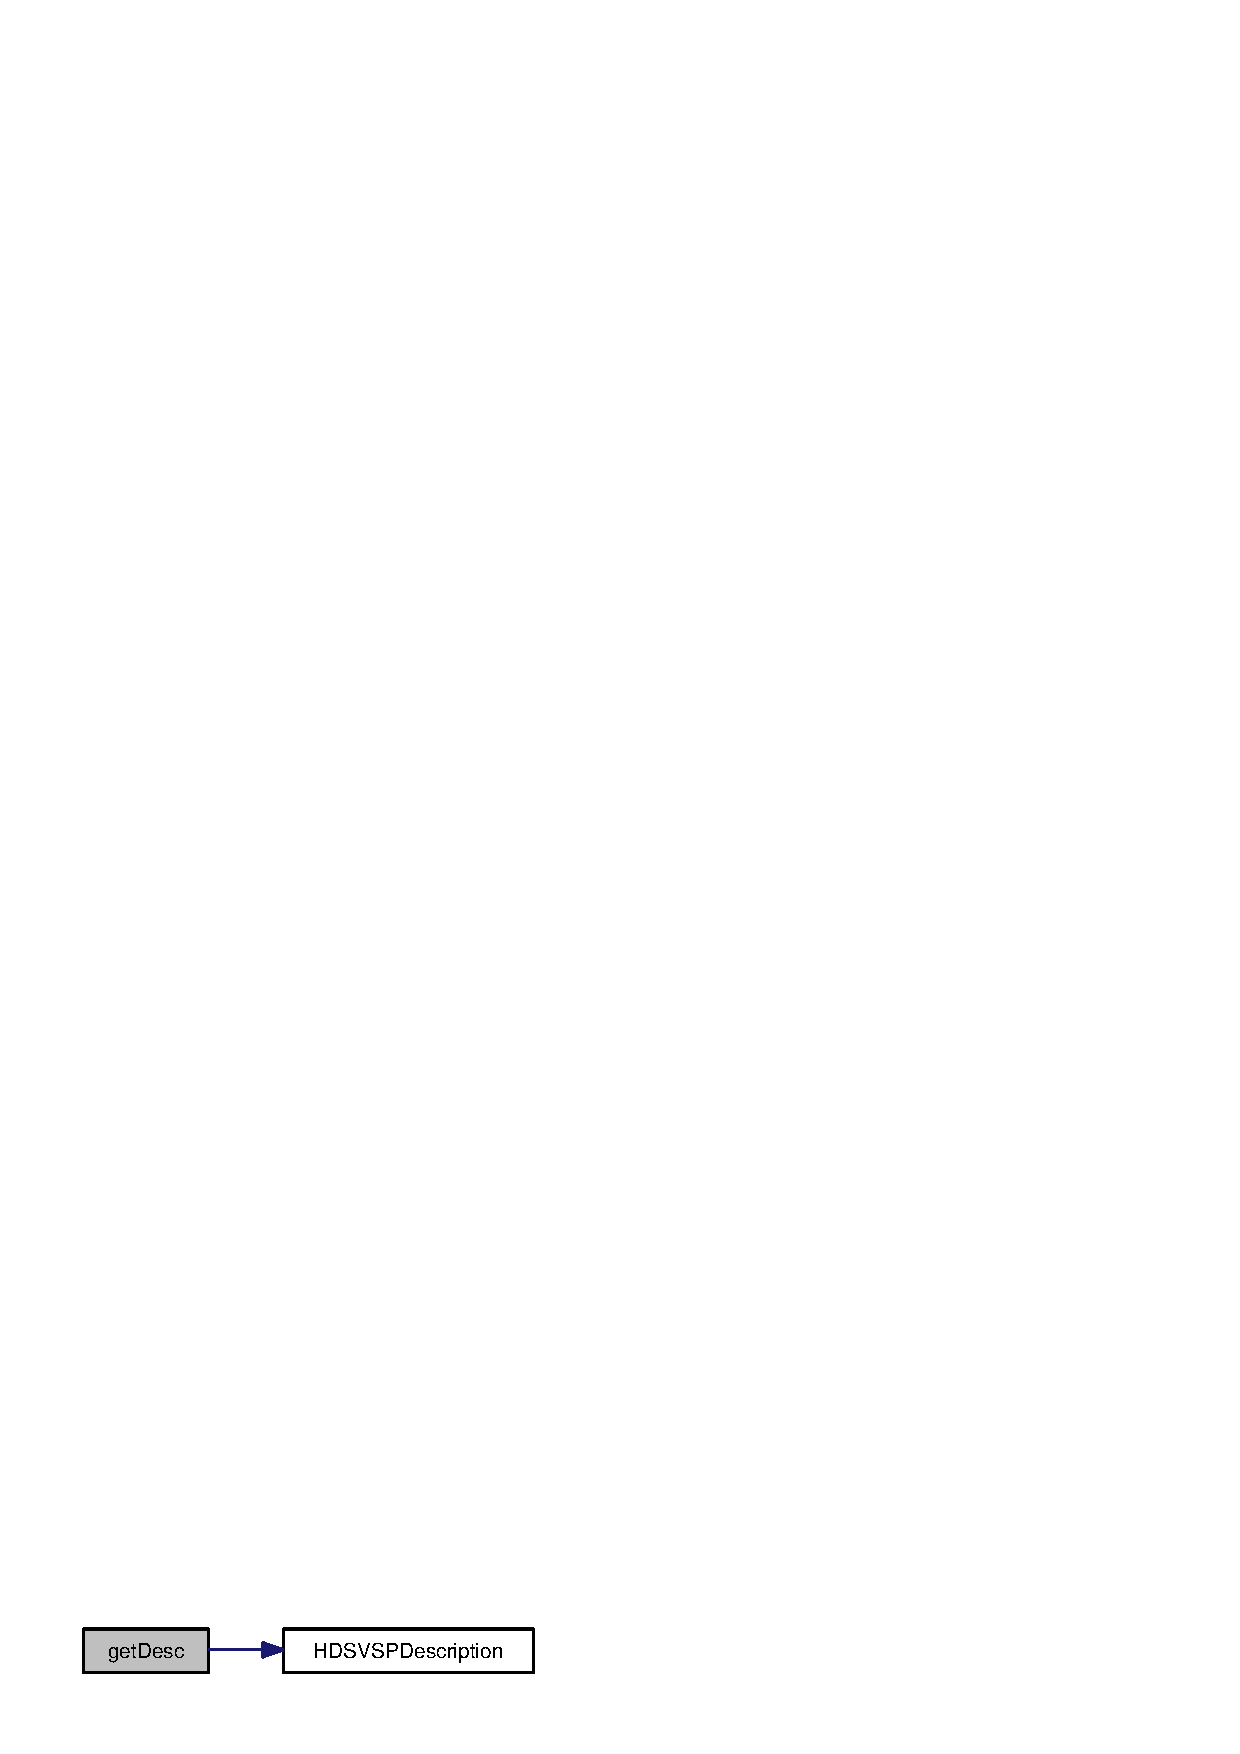
\includegraphics[width=260pt]{classorg_1_1smallfoot_1_1wwn_1_1HDSVSPDescription_a7e34be4d9bd11a9971c007c6231b8c01_cgraph}
\end{center}
\end{figure}


\index{org\-::smallfoot\-::wwn\-::\-H\-D\-S\-V\-S\-P\-Description@{org\-::smallfoot\-::wwn\-::\-H\-D\-S\-V\-S\-P\-Description}!to\-String@{to\-String}}
\index{to\-String@{to\-String}!org::smallfoot::wwn::HDSVSPDescription@{org\-::smallfoot\-::wwn\-::\-H\-D\-S\-V\-S\-P\-Description}}
\subsubsection[{to\-String}]{\setlength{\rightskip}{0pt plus 5cm}String to\-String (
\begin{DoxyParamCaption}
{}
\end{DoxyParamCaption}
)\hspace{0.3cm}{\ttfamily [inline]}}\label{classorg_1_1smallfoot_1_1wwn_1_1HDSVSPDescription_ad146fa8579a5f8a876c4688cc5a68520}


return a description or alias for this W\-W\-N; if brief is set to true during the call to \doxyref{get\-Desc()}{p.}{classorg_1_1smallfoot_1_1wwn_1_1HDSVSPDescription_a7e34be4d9bd11a9971c007c6231b8c01}, then a shorter description or alias will be returned 

\begin{DoxySeeAlso}{See Also}
\doxyref{get\-Desc(boolean,boolean,\-String)}{p.}{classorg_1_1smallfoot_1_1wwn_1_1HDSVSPDescription_a7e34be4d9bd11a9971c007c6231b8c01}
\end{DoxySeeAlso}
\begin{DoxyReturn}{Returns}
generated alias or nickname for the W\-W\-N 
\end{DoxyReturn}
\begin{DoxyRefDesc}{Todo}
\item[{\bf Todo}]50060e8\-: 005\-: U\-S\-P-\/\-V\-: {\tt http\-://www.\-hitachi-\/storage.\-com/content/how-\/decode-\/usp-\/v-\/wwn} 00/5\-: U\-S\-P-\/\-V\-: brionetka.\-com/linux/?p=38 breaks it up as N\-O\-O\-O\-O\-O\-O\-F\-F\-S\-S\-S\-S\-C\-P (N=5, O\-O\-O\-O\-O\-O = O\-U\-I, F\-F = Family \{01=7700/\-Lightning, 02=9900/\-Thunder\}, S\-S\-S\-S=Serial, C = Cluster, P=Port (0-\/\-F=A-\/\-Q skipping \char`\"{}\-I\char`\"{}) note article confuses N\-A\-A marker as \char`\"{}50\char`\"{} need to check against {\tt http\-://p2v.\-it/tools/wwndec/index.\-php?input=50060\-E8010277210} need to check {\tt http\-://p2v.\-it/tools/wwndec/index.\-php?input=50060e8016624800} \end{DoxyRefDesc}


Definition at line 46 of file H\-D\-S\-V\-S\-P\-Description.\-java.



The documentation for this class was generated from the following file\-:\begin{DoxyCompactItemize}
\item 
java/{\bf H\-D\-S\-V\-S\-P\-Description.\-java}\end{DoxyCompactItemize}

\section{H\-P3\-Par\-Description Class Reference}
\label{classorg_1_1smallfoot_1_1wwn_1_1HP3ParDescription}\index{H\-P3\-Par\-Description@{H\-P3\-Par\-Description}}


Inheritance diagram for H\-P3\-Par\-Description\-:\nopagebreak
\begin{figure}[H]
\begin{center}
\leavevmode
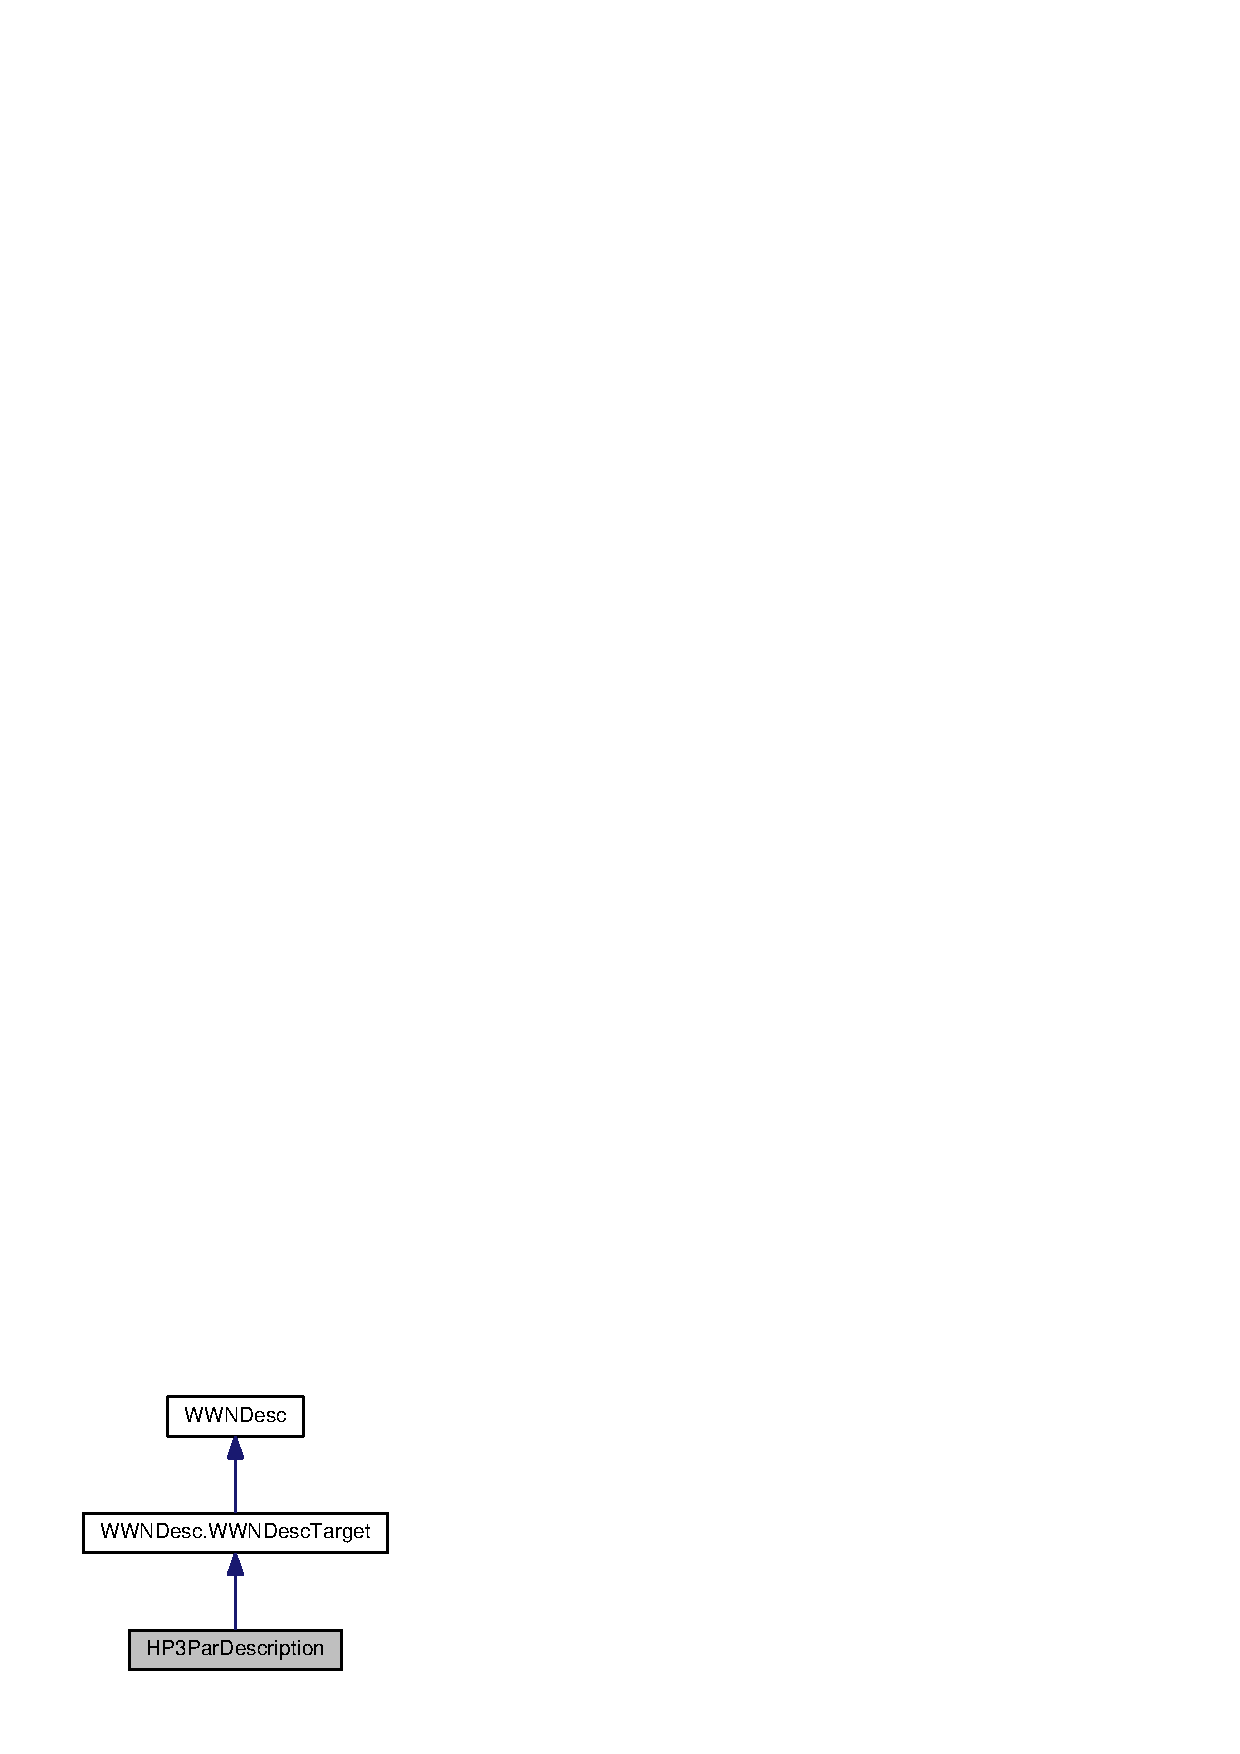
\includegraphics[width=158pt]{classorg_1_1smallfoot_1_1wwn_1_1HP3ParDescription__inherit__graph}
\end{center}
\end{figure}


Collaboration diagram for H\-P3\-Par\-Description\-:\nopagebreak
\begin{figure}[H]
\begin{center}
\leavevmode
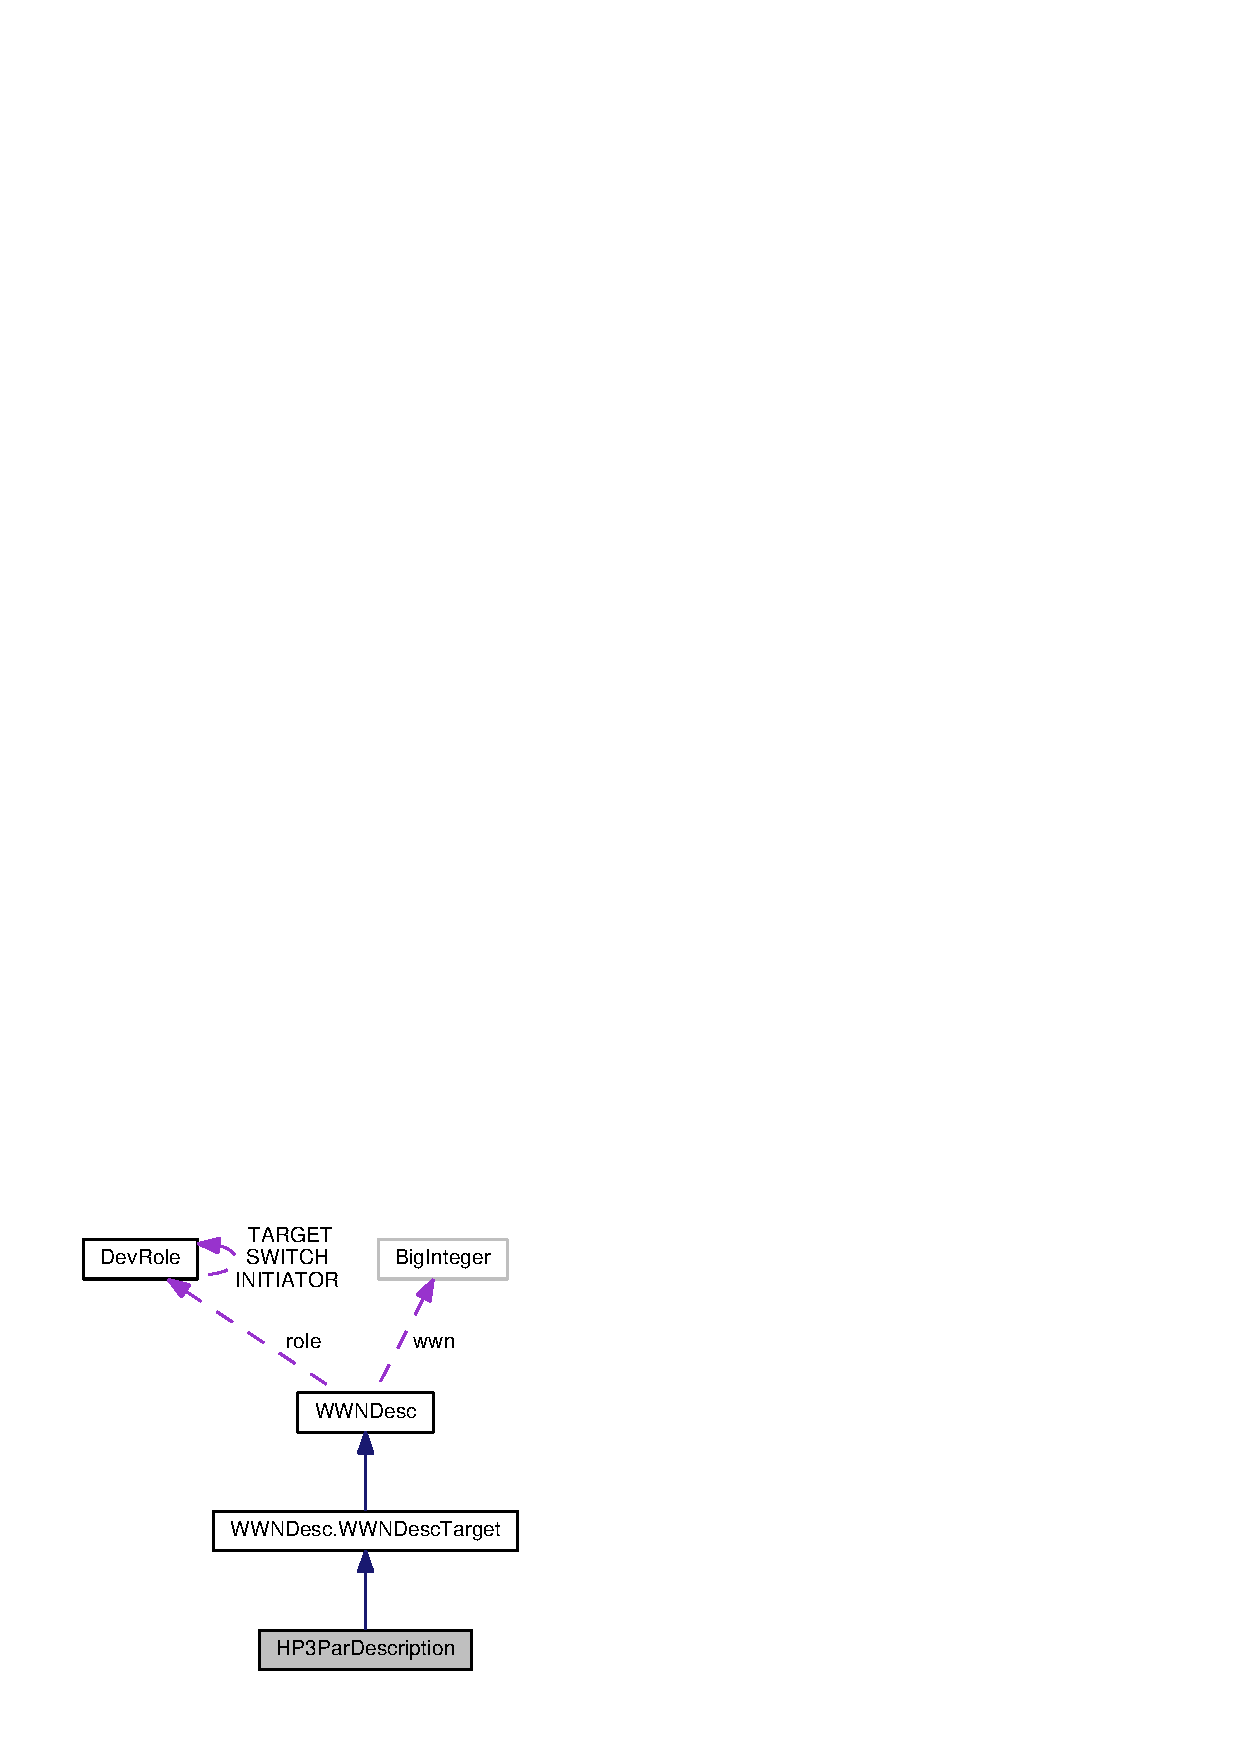
\includegraphics[width=158pt]{classorg_1_1smallfoot_1_1wwn_1_1HP3ParDescription__coll__graph}
\end{center}
\end{figure}
\subsection*{Public Member Functions}
\begin{DoxyCompactItemize}
\item 
{\bf H\-P3\-Par\-Description} (String wwn)
\begin{DoxyCompactList}\small\item\em create an instance with this.\-brief set to false. \end{DoxyCompactList}\item 
{\bf H\-P3\-Par\-Description} (boolean brief, String wwn)
\begin{DoxyCompactList}\small\item\em create an instance with the given W\-W\-N. \end{DoxyCompactList}\item 
String {\bf to\-String} ()
\begin{DoxyCompactList}\small\item\em return a description or alias for this W\-W\-N \end{DoxyCompactList}\end{DoxyCompactItemize}
\subsection*{Static Public Member Functions}
\begin{DoxyCompactItemize}
\item 
static {\bf W\-W\-N\-Desc} {\bf get\-Desc} (boolean strong, boolean brief, String wwn)
\begin{DoxyCompactList}\small\item\em If this class matches or describes the given W\-W\-N, returns a new instance of this class loaded with the given W\-W\-N. \end{DoxyCompactList}\end{DoxyCompactItemize}


\subsection{Detailed Description}


Definition at line 10 of file H\-P3\-Par\-Description.\-java.



\subsection{Constructor \& Destructor Documentation}
\index{org\-::smallfoot\-::wwn\-::\-H\-P3\-Par\-Description@{org\-::smallfoot\-::wwn\-::\-H\-P3\-Par\-Description}!H\-P3\-Par\-Description@{H\-P3\-Par\-Description}}
\index{H\-P3\-Par\-Description@{H\-P3\-Par\-Description}!org::smallfoot::wwn::HP3ParDescription@{org\-::smallfoot\-::wwn\-::\-H\-P3\-Par\-Description}}
\subsubsection[{H\-P3\-Par\-Description}]{\setlength{\rightskip}{0pt plus 5cm}{\bf H\-P3\-Par\-Description} (
\begin{DoxyParamCaption}
\item[{String}]{wwn}
\end{DoxyParamCaption}
)\hspace{0.3cm}{\ttfamily [inline]}}\label{classorg_1_1smallfoot_1_1wwn_1_1HP3ParDescription_a8113b7e0db585cec11c121463692764e}


create an instance with this.\-brief set to false. 

This is a convenience function to support the older constructor model


\begin{DoxyParams}{Parameters}
{\em wwn} & the W\-W\-N to evaluate and describe \\
\hline
\end{DoxyParams}


Definition at line 13 of file H\-P3\-Par\-Description.\-java.



Referenced by H\-P3\-Par\-Description.\-get\-Desc().

\index{org\-::smallfoot\-::wwn\-::\-H\-P3\-Par\-Description@{org\-::smallfoot\-::wwn\-::\-H\-P3\-Par\-Description}!H\-P3\-Par\-Description@{H\-P3\-Par\-Description}}
\index{H\-P3\-Par\-Description@{H\-P3\-Par\-Description}!org::smallfoot::wwn::HP3ParDescription@{org\-::smallfoot\-::wwn\-::\-H\-P3\-Par\-Description}}
\subsubsection[{H\-P3\-Par\-Description}]{\setlength{\rightskip}{0pt plus 5cm}{\bf H\-P3\-Par\-Description} (
\begin{DoxyParamCaption}
\item[{boolean}]{brief, }
\item[{String}]{wwn}
\end{DoxyParamCaption}
)\hspace{0.3cm}{\ttfamily [inline]}}\label{classorg_1_1smallfoot_1_1wwn_1_1HP3ParDescription_a06ba9718f7c87d200769170c5b6b3e83}


create an instance with the given W\-W\-N. 

Values given to the constructor are simply copied to internal variables for later use


\begin{DoxyParams}{Parameters}
{\em brief} & whether an abbreviated description is requested \\
\hline
{\em wwn} & the W\-W\-N to evaluate and describe \\
\hline
\end{DoxyParams}


Definition at line 18 of file H\-P3\-Par\-Description.\-java.



\subsection{Member Function Documentation}
\index{org\-::smallfoot\-::wwn\-::\-H\-P3\-Par\-Description@{org\-::smallfoot\-::wwn\-::\-H\-P3\-Par\-Description}!get\-Desc@{get\-Desc}}
\index{get\-Desc@{get\-Desc}!org::smallfoot::wwn::HP3ParDescription@{org\-::smallfoot\-::wwn\-::\-H\-P3\-Par\-Description}}
\subsubsection[{get\-Desc}]{\setlength{\rightskip}{0pt plus 5cm}static {\bf W\-W\-N\-Desc} get\-Desc (
\begin{DoxyParamCaption}
\item[{boolean}]{strong, }
\item[{boolean}]{brief, }
\item[{String}]{wwn}
\end{DoxyParamCaption}
)\hspace{0.3cm}{\ttfamily [inline]}, {\ttfamily [static]}}\label{classorg_1_1smallfoot_1_1wwn_1_1HP3ParDescription_a7e34be4d9bd11a9971c007c6231b8c01}


If this class matches or describes the given W\-W\-N, returns a new instance of this class loaded with the given W\-W\-N. 

\begin{DoxyReturn}{Returns}
new instance of this class, or null if the given wwn does not match this class 
\end{DoxyReturn}

\begin{DoxyParams}{Parameters}
{\em strong} & is ignored\-: this class is a strong representation, not a weak one based on empirical matching, hence can always be used with confidence \\
\hline
{\em brief} & is ignored\-: this class has only one representation of the W\-W\-N description or alias \\
\hline
{\em wwn} & the W\-W\-N (W\-W\-P\-N or W\-W\-N\-N, but typically W\-W\-P\-N) to match \\
\hline
\end{DoxyParams}


Definition at line 31 of file H\-P3\-Par\-Description.\-java.



References H\-P3\-Par\-Description.\-H\-P3\-Par\-Description().



Referenced by W\-W\-N\-Description.\-get\-W\-W\-N\-Descriptor().



Here is the call graph for this function\-:\nopagebreak
\begin{figure}[H]
\begin{center}
\leavevmode
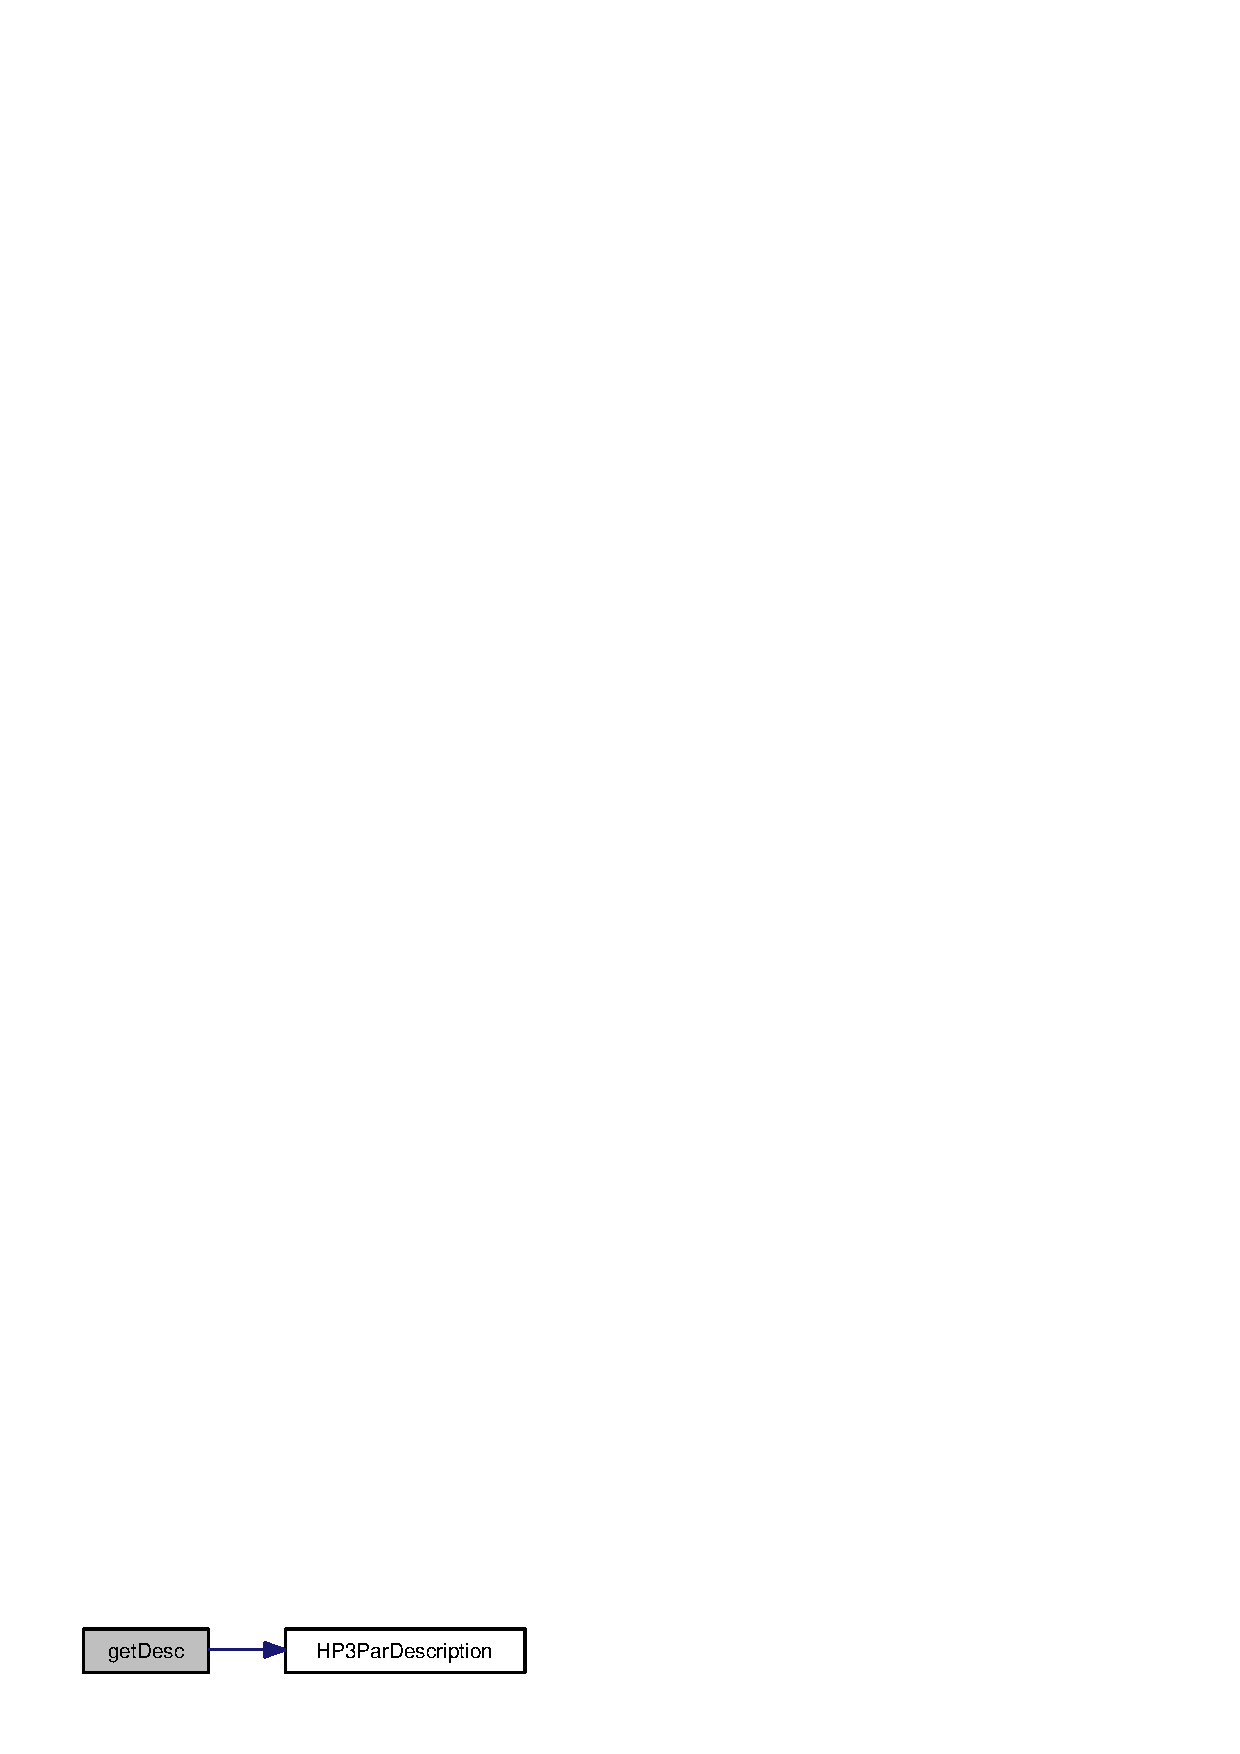
\includegraphics[width=256pt]{classorg_1_1smallfoot_1_1wwn_1_1HP3ParDescription_a7e34be4d9bd11a9971c007c6231b8c01_cgraph}
\end{center}
\end{figure}


\index{org\-::smallfoot\-::wwn\-::\-H\-P3\-Par\-Description@{org\-::smallfoot\-::wwn\-::\-H\-P3\-Par\-Description}!to\-String@{to\-String}}
\index{to\-String@{to\-String}!org::smallfoot::wwn::HP3ParDescription@{org\-::smallfoot\-::wwn\-::\-H\-P3\-Par\-Description}}
\subsubsection[{to\-String}]{\setlength{\rightskip}{0pt plus 5cm}String to\-String (
\begin{DoxyParamCaption}
{}
\end{DoxyParamCaption}
)\hspace{0.3cm}{\ttfamily [inline]}}\label{classorg_1_1smallfoot_1_1wwn_1_1HP3ParDescription_ad146fa8579a5f8a876c4688cc5a68520}


return a description or alias for this W\-W\-N 

\begin{DoxyReturn}{Returns}
generated alias or nickname for the W\-W\-N 
\end{DoxyReturn}


Definition at line 44 of file H\-P3\-Par\-Description.\-java.



The documentation for this class was generated from the following file\-:\begin{DoxyCompactItemize}
\item 
java/{\bf H\-P3\-Par\-Description.\-java}\end{DoxyCompactItemize}

\section{\-H\-P\-Dot\-Hill\-Description \-Class \-Reference}
\label{classorg_1_1smallfoot_1_1wwn_1_1HPDotHillDescription}\index{\-H\-P\-Dot\-Hill\-Description@{\-H\-P\-Dot\-Hill\-Description}}


\-Descriptor for (\-Dot \-Hill \-Systems \-Modular \-Smart \-Array) \-H\-P \-P2000.  




\-Inheritance diagram for \-H\-P\-Dot\-Hill\-Description\-:\nopagebreak
\begin{figure}[H]
\begin{center}
\leavevmode
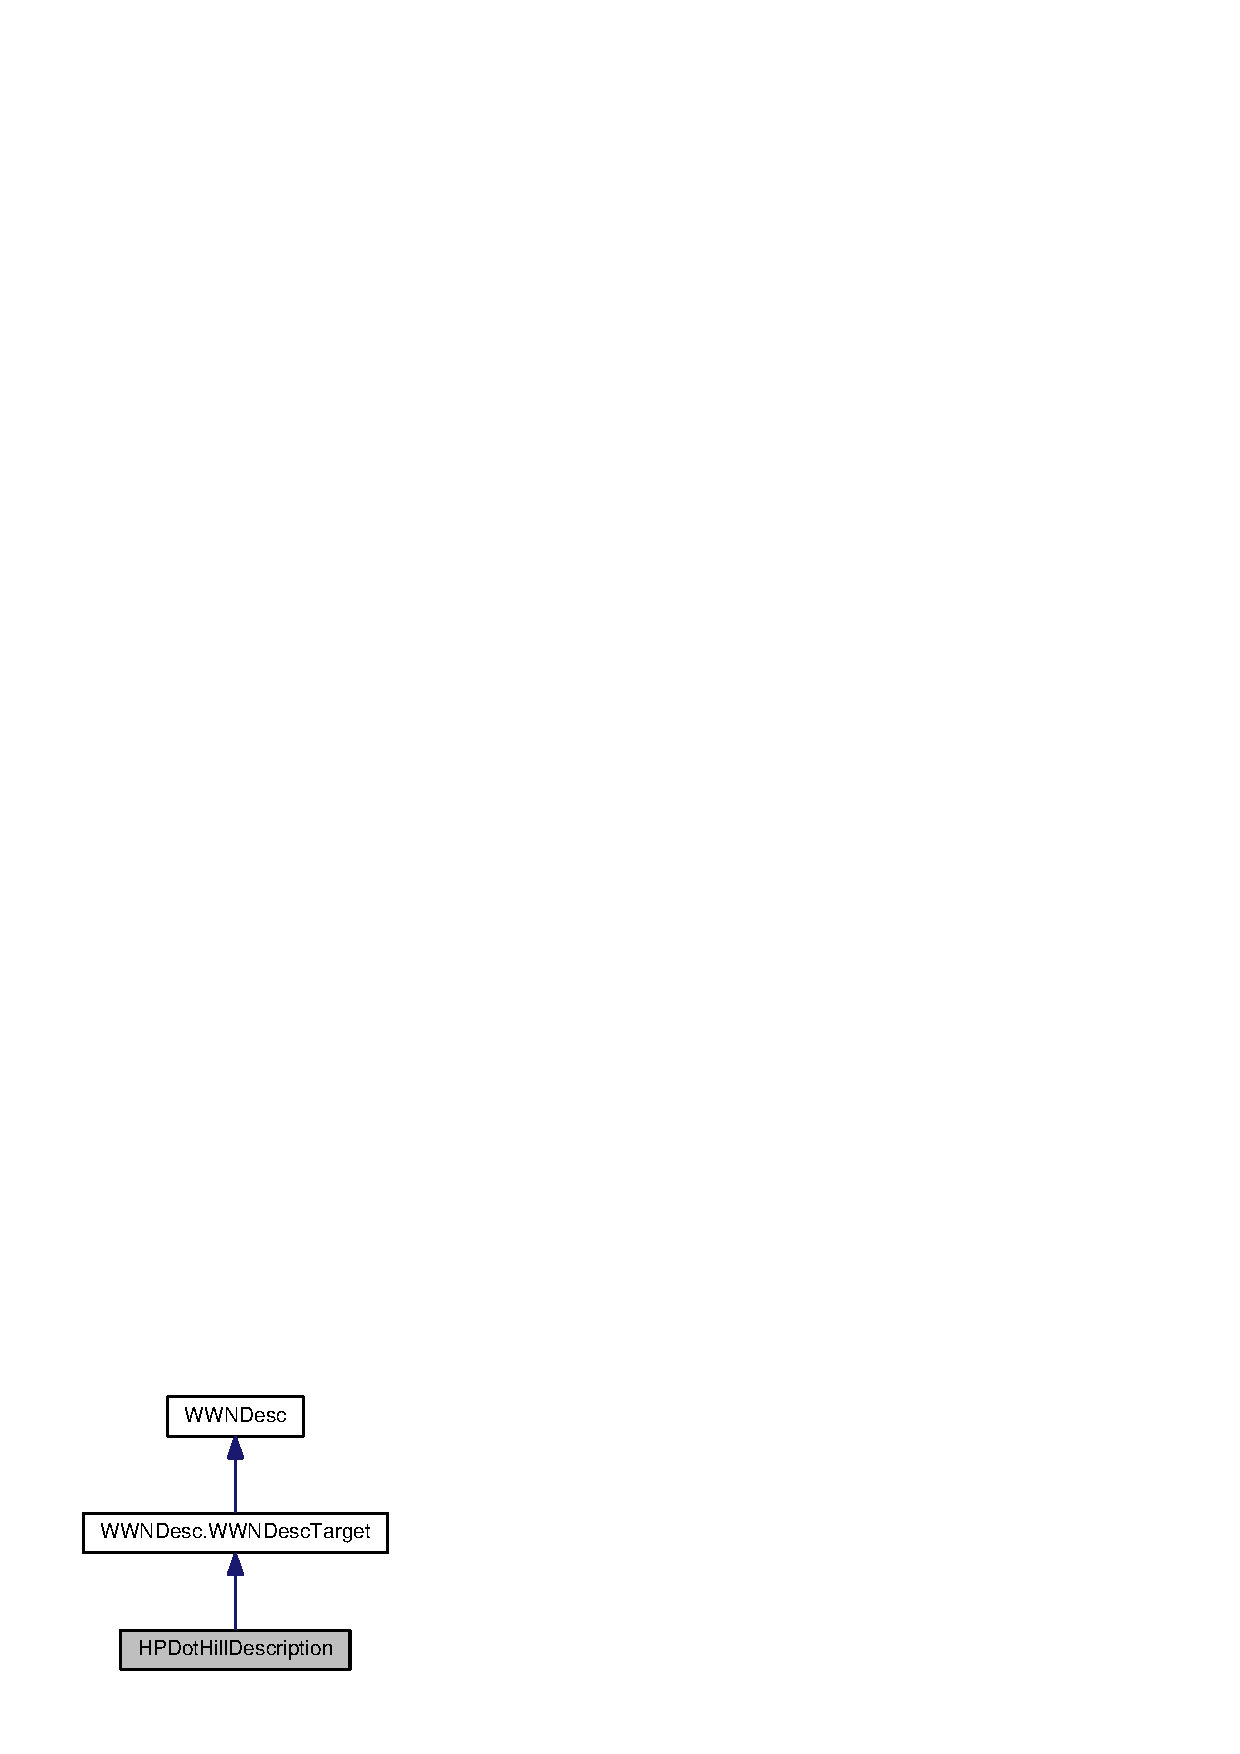
\includegraphics[width=170pt]{classorg_1_1smallfoot_1_1wwn_1_1HPDotHillDescription__inherit__graph}
\end{center}
\end{figure}


\-Collaboration diagram for \-H\-P\-Dot\-Hill\-Description\-:\nopagebreak
\begin{figure}[H]
\begin{center}
\leavevmode
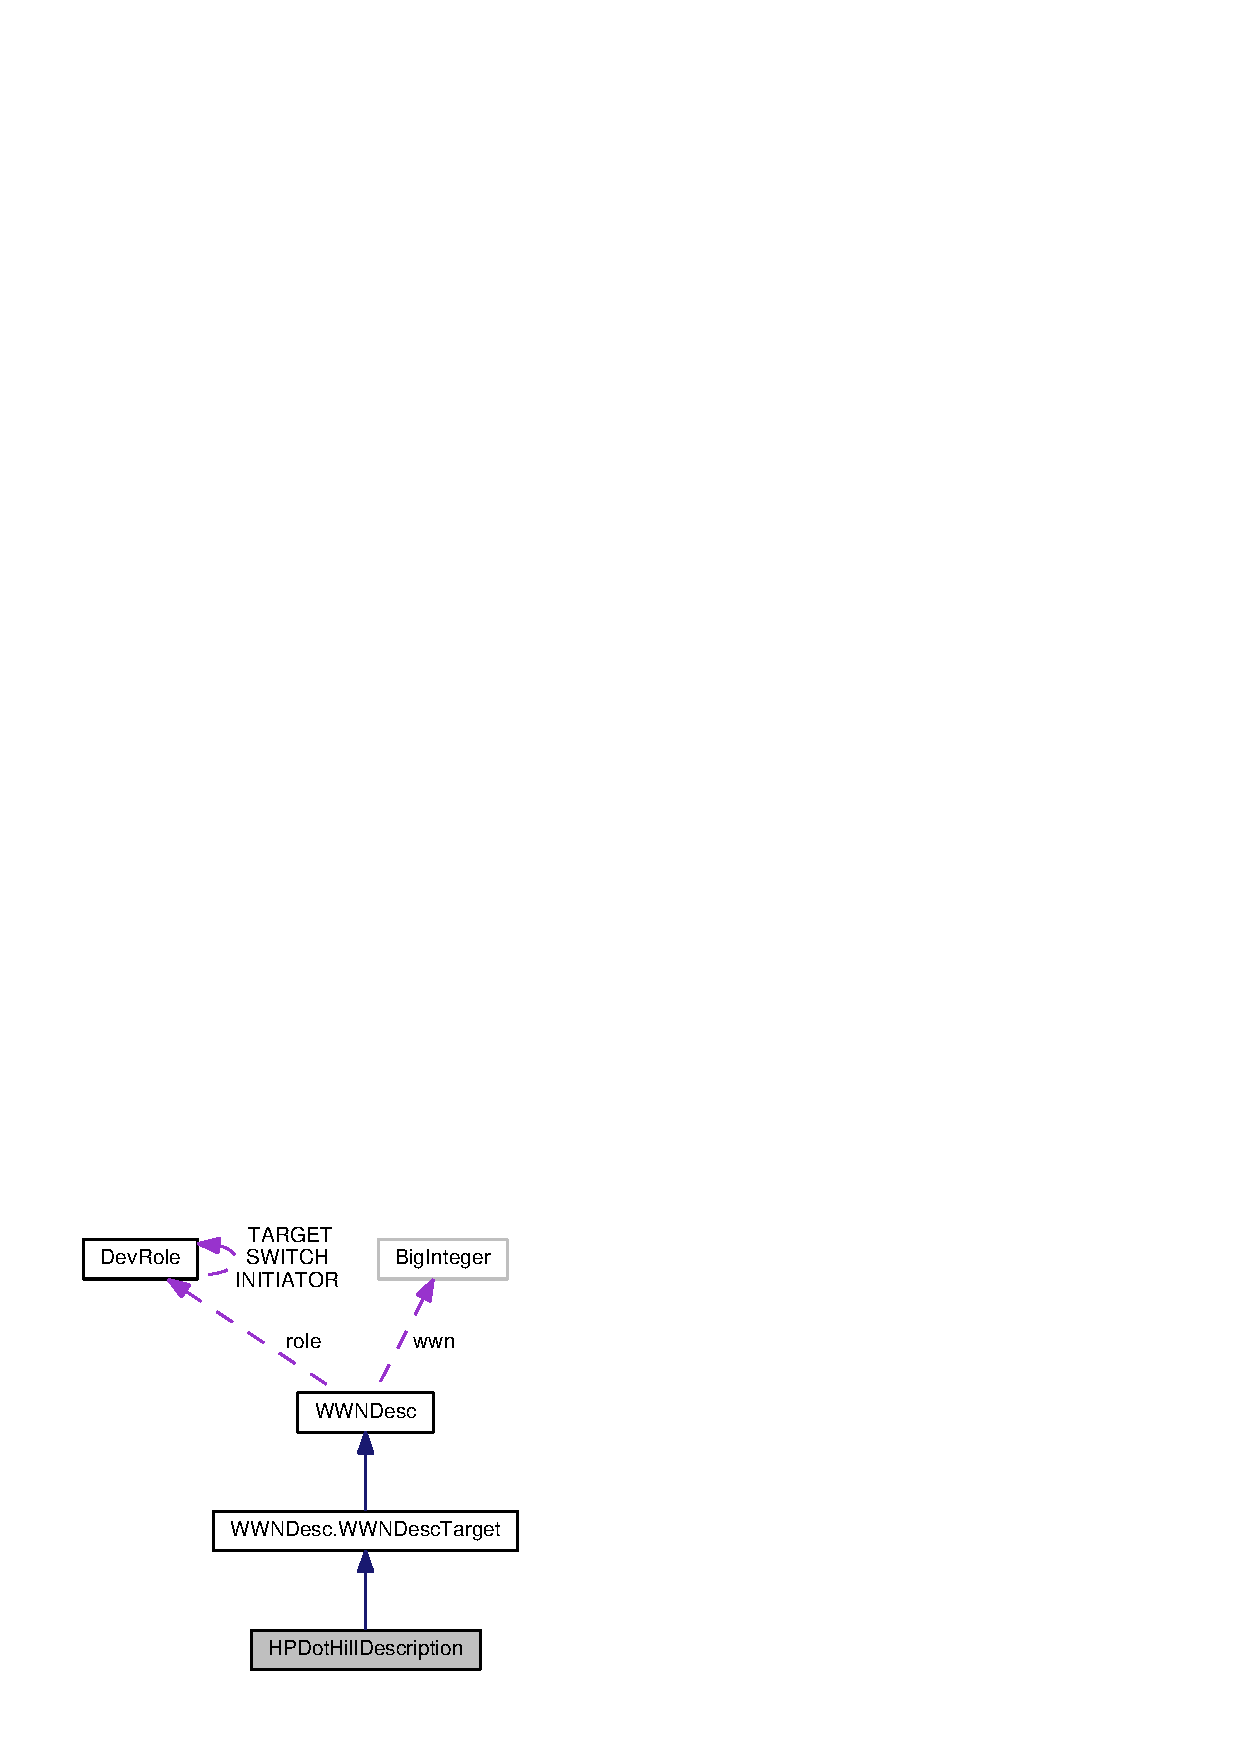
\includegraphics[width=170pt]{classorg_1_1smallfoot_1_1wwn_1_1HPDotHillDescription__coll__graph}
\end{center}
\end{figure}
\subsection*{\-Public \-Member \-Functions}
\begin{DoxyCompactItemize}
\item 
{\bf \-H\-P\-Dot\-Hill\-Description} (\-String {\bf wwn})
\item 
\-String {\bf to\-String} ()
\end{DoxyCompactItemize}
\subsection*{\-Static \-Public \-Member \-Functions}
\begin{DoxyCompactItemize}
\item 
static {\bf \-W\-W\-N\-Desc} {\bf get\-Desc} (booleanstrong, boolean {\bf brief}, \-String {\bf wwn})
\end{DoxyCompactItemize}


\subsection{\-Detailed \-Description}
\-Descriptor for (\-Dot \-Hill \-Systems \-Modular \-Smart \-Array) \-H\-P \-P2000. 

\-These descriptors are fairly weak\-: \-I'm somewhat sure of the serial, but only two matches for the port-\/number logic. 

\-Definition at line 15 of file \-H\-P\-Dot\-Hill\-Description.\-java.



\subsection{\-Constructor \& \-Destructor \-Documentation}
\index{org\-::smallfoot\-::wwn\-::\-H\-P\-Dot\-Hill\-Description@{org\-::smallfoot\-::wwn\-::\-H\-P\-Dot\-Hill\-Description}!\-H\-P\-Dot\-Hill\-Description@{\-H\-P\-Dot\-Hill\-Description}}
\index{\-H\-P\-Dot\-Hill\-Description@{\-H\-P\-Dot\-Hill\-Description}!org::smallfoot::wwn::HPDotHillDescription@{org\-::smallfoot\-::wwn\-::\-H\-P\-Dot\-Hill\-Description}}
\subsubsection[{\-H\-P\-Dot\-Hill\-Description}]{\setlength{\rightskip}{0pt plus 5cm}{\bf \-H\-P\-Dot\-Hill\-Description} (
\begin{DoxyParamCaption}
\item[{\-String}]{wwn}
\end{DoxyParamCaption}
)\hspace{0.3cm}{\ttfamily  [inline]}}\label{classorg_1_1smallfoot_1_1wwn_1_1HPDotHillDescription_ad22528e257f239b38e608c80cd4806a6}


\-Definition at line 17 of file \-H\-P\-Dot\-Hill\-Description.\-java.



\-Referenced by \-H\-P\-Dot\-Hill\-Description.\-get\-Desc().



\subsection{\-Member \-Function \-Documentation}
\index{org\-::smallfoot\-::wwn\-::\-H\-P\-Dot\-Hill\-Description@{org\-::smallfoot\-::wwn\-::\-H\-P\-Dot\-Hill\-Description}!get\-Desc@{get\-Desc}}
\index{get\-Desc@{get\-Desc}!org::smallfoot::wwn::HPDotHillDescription@{org\-::smallfoot\-::wwn\-::\-H\-P\-Dot\-Hill\-Description}}
\subsubsection[{get\-Desc}]{\setlength{\rightskip}{0pt plus 5cm}static {\bf \-W\-W\-N\-Desc} {\bf get\-Desc} (
\begin{DoxyParamCaption}
\item[{boolean}]{strong, }
\item[{boolean}]{brief, }
\item[{\-String}]{wwn}
\end{DoxyParamCaption}
)\hspace{0.3cm}{\ttfamily  [inline, static]}}\label{classorg_1_1smallfoot_1_1wwn_1_1HPDotHillDescription_a22e37e33bddb34b1c7506f3f35749eb2}


\-Definition at line 22 of file \-H\-P\-Dot\-Hill\-Description.\-java.



\-References \-H\-P\-Dot\-Hill\-Description.\-H\-P\-Dot\-Hill\-Description().



\-Referenced by \-W\-W\-N\-Description.\-get\-W\-W\-N\-Descriptor().



\-Here is the call graph for this function\-:\nopagebreak
\begin{figure}[H]
\begin{center}
\leavevmode
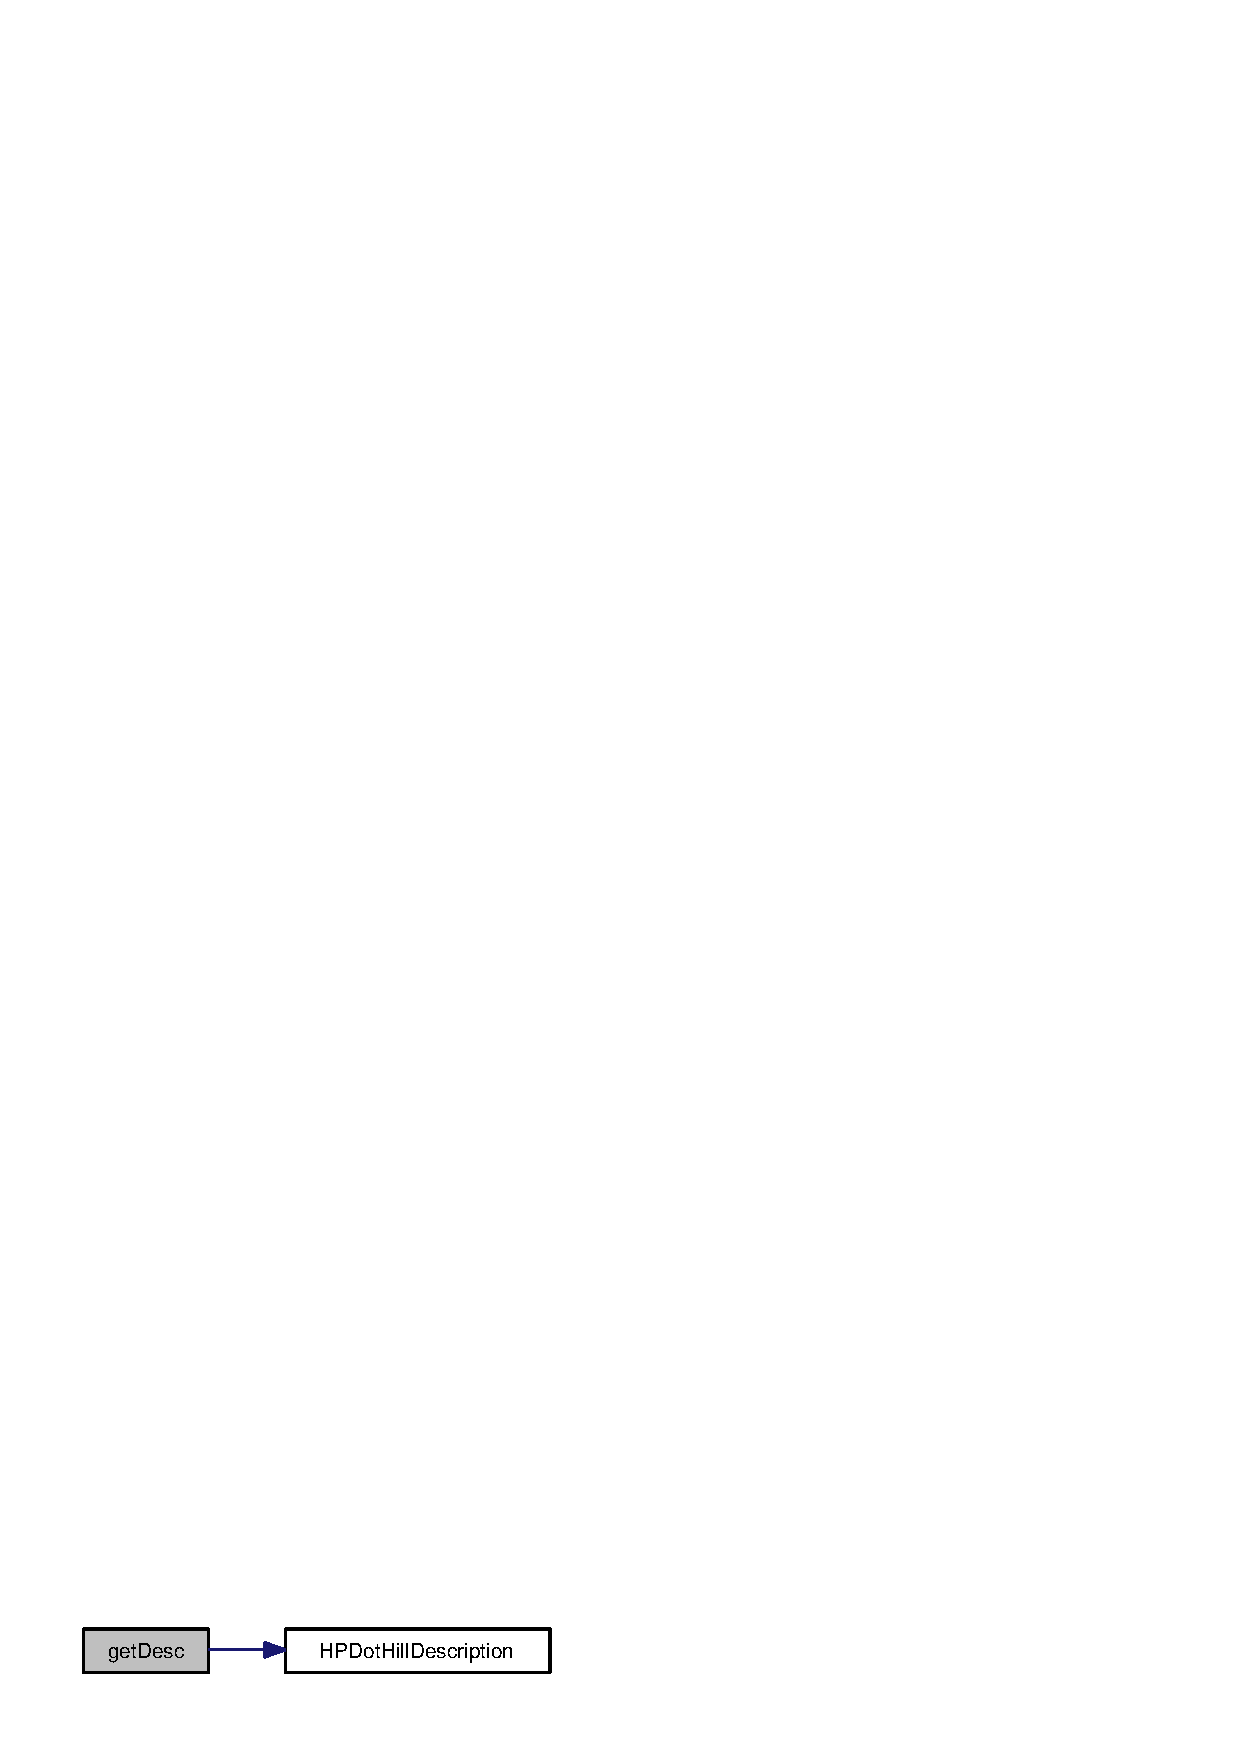
\includegraphics[width=268pt]{classorg_1_1smallfoot_1_1wwn_1_1HPDotHillDescription_a22e37e33bddb34b1c7506f3f35749eb2_cgraph}
\end{center}
\end{figure}


\index{org\-::smallfoot\-::wwn\-::\-H\-P\-Dot\-Hill\-Description@{org\-::smallfoot\-::wwn\-::\-H\-P\-Dot\-Hill\-Description}!to\-String@{to\-String}}
\index{to\-String@{to\-String}!org::smallfoot::wwn::HPDotHillDescription@{org\-::smallfoot\-::wwn\-::\-H\-P\-Dot\-Hill\-Description}}
\subsubsection[{to\-String}]{\setlength{\rightskip}{0pt plus 5cm}\-String {\bf to\-String} (
\begin{DoxyParamCaption}
{}
\end{DoxyParamCaption}
)\hspace{0.3cm}{\ttfamily  [inline]}}\label{classorg_1_1smallfoot_1_1wwn_1_1HPDotHillDescription_ad146fa8579a5f8a876c4688cc5a68520}


\-Reimplemented from {\bf \-W\-W\-N\-Desc} \doxyref{}{p.}{classorg_1_1smallfoot_1_1wwn_1_1WWNDesc_ad146fa8579a5f8a876c4688cc5a68520}.



\-Definition at line 30 of file \-H\-P\-Dot\-Hill\-Description.\-java.



\-References \-W\-W\-N\-Desc.\-wwn.



\-The documentation for this class was generated from the following file\-:\begin{DoxyCompactItemize}
\item 
java/{\bf \-H\-P\-Dot\-Hill\-Description.\-java}\end{DoxyCompactItemize}

\section{I\+B\+M3700\+Description Class Reference}
\label{classorg_1_1smallfoot_1_1wwn_1_1IBM3700Description}\index{I\+B\+M3700\+Description@{I\+B\+M3700\+Description}}


\doxyref{I\+B\+M3700\+Description}{p.}{classorg_1_1smallfoot_1_1wwn_1_1IBM3700Description} (ie Ram\+San-\/\+G8332-\/\+F\+C-\/2\+B) breaks out the serial and port information from the Texas Memory Systems hardware initially called Ram\+San.  




Inheritance diagram for I\+B\+M3700\+Description\+:\nopagebreak
\begin{figure}[H]
\begin{center}
\leavevmode
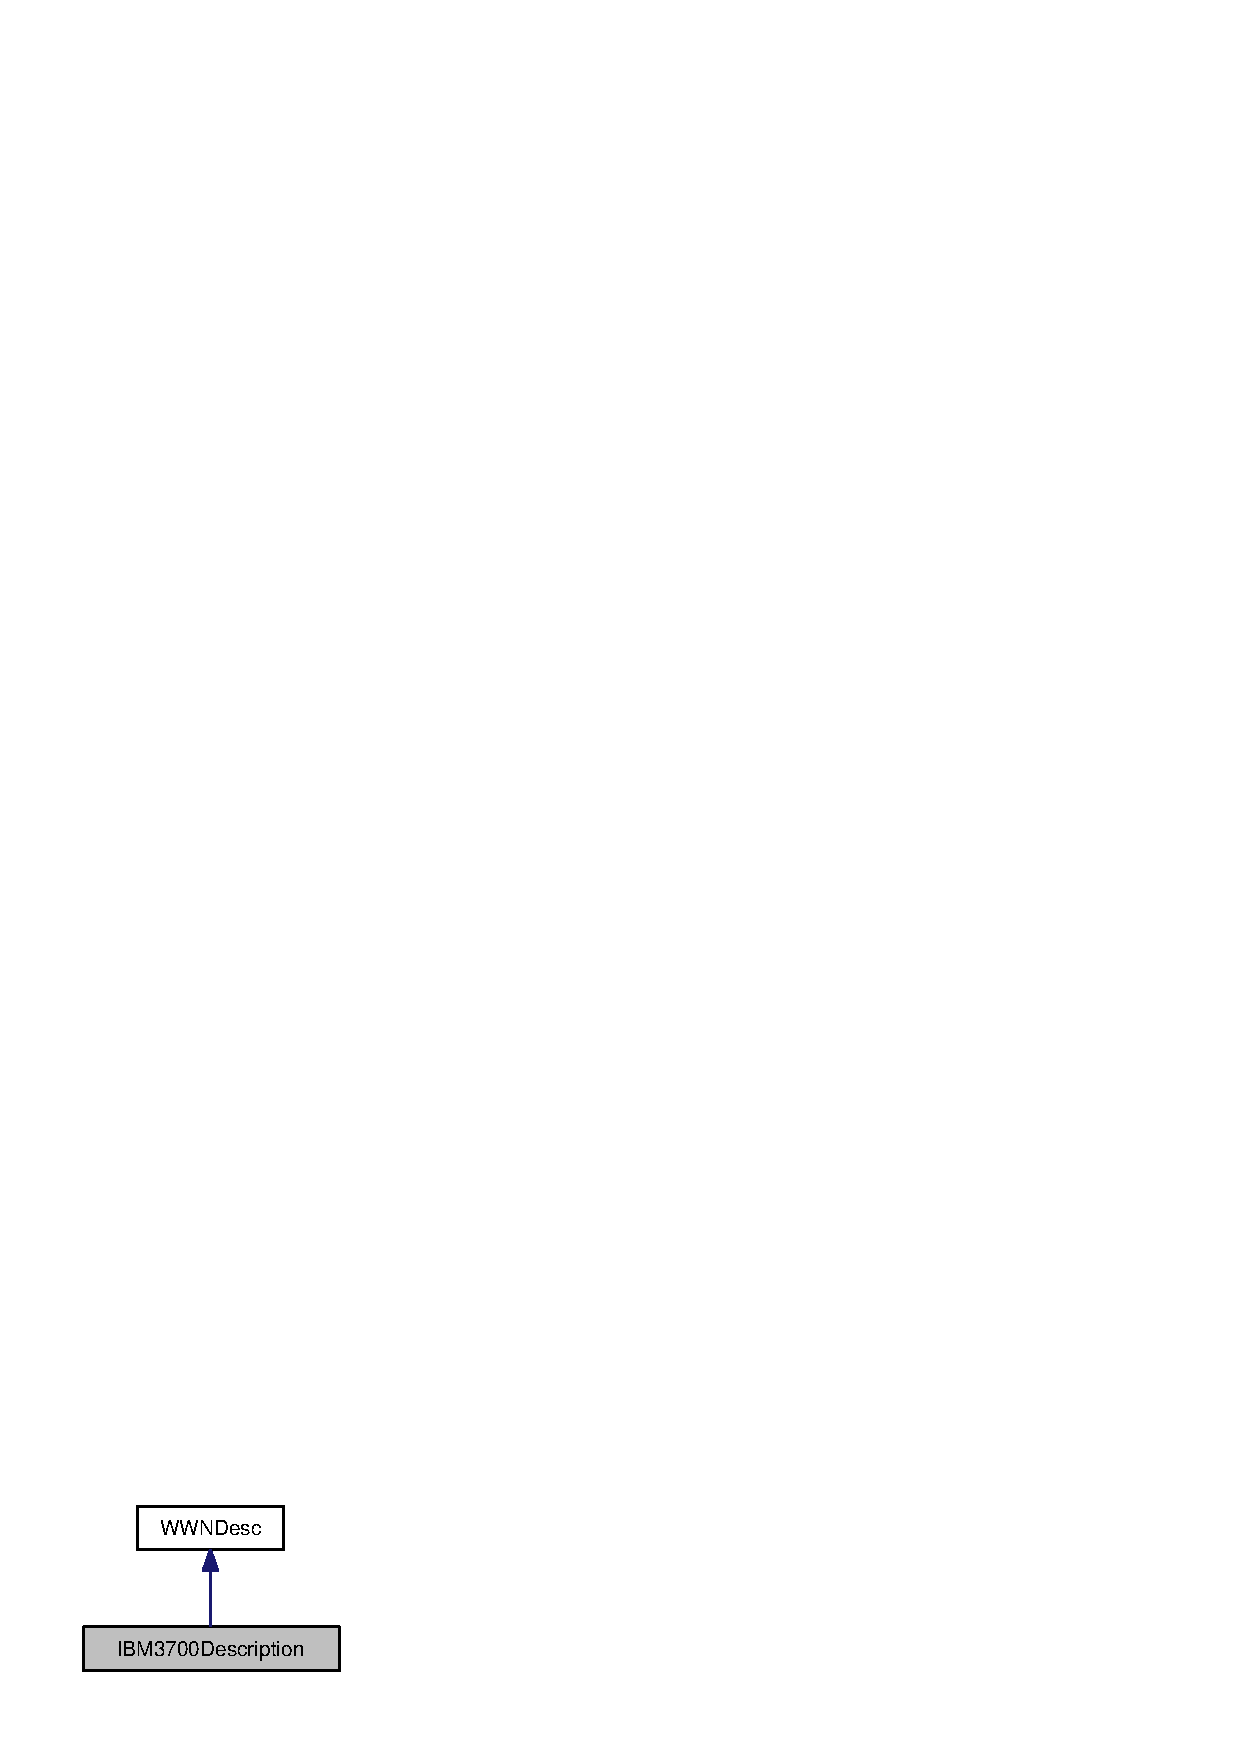
\includegraphics[width=188pt]{classorg_1_1smallfoot_1_1wwn_1_1IBM3700Description__inherit__graph}
\end{center}
\end{figure}


Collaboration diagram for I\+B\+M3700\+Description\+:\nopagebreak
\begin{figure}[H]
\begin{center}
\leavevmode
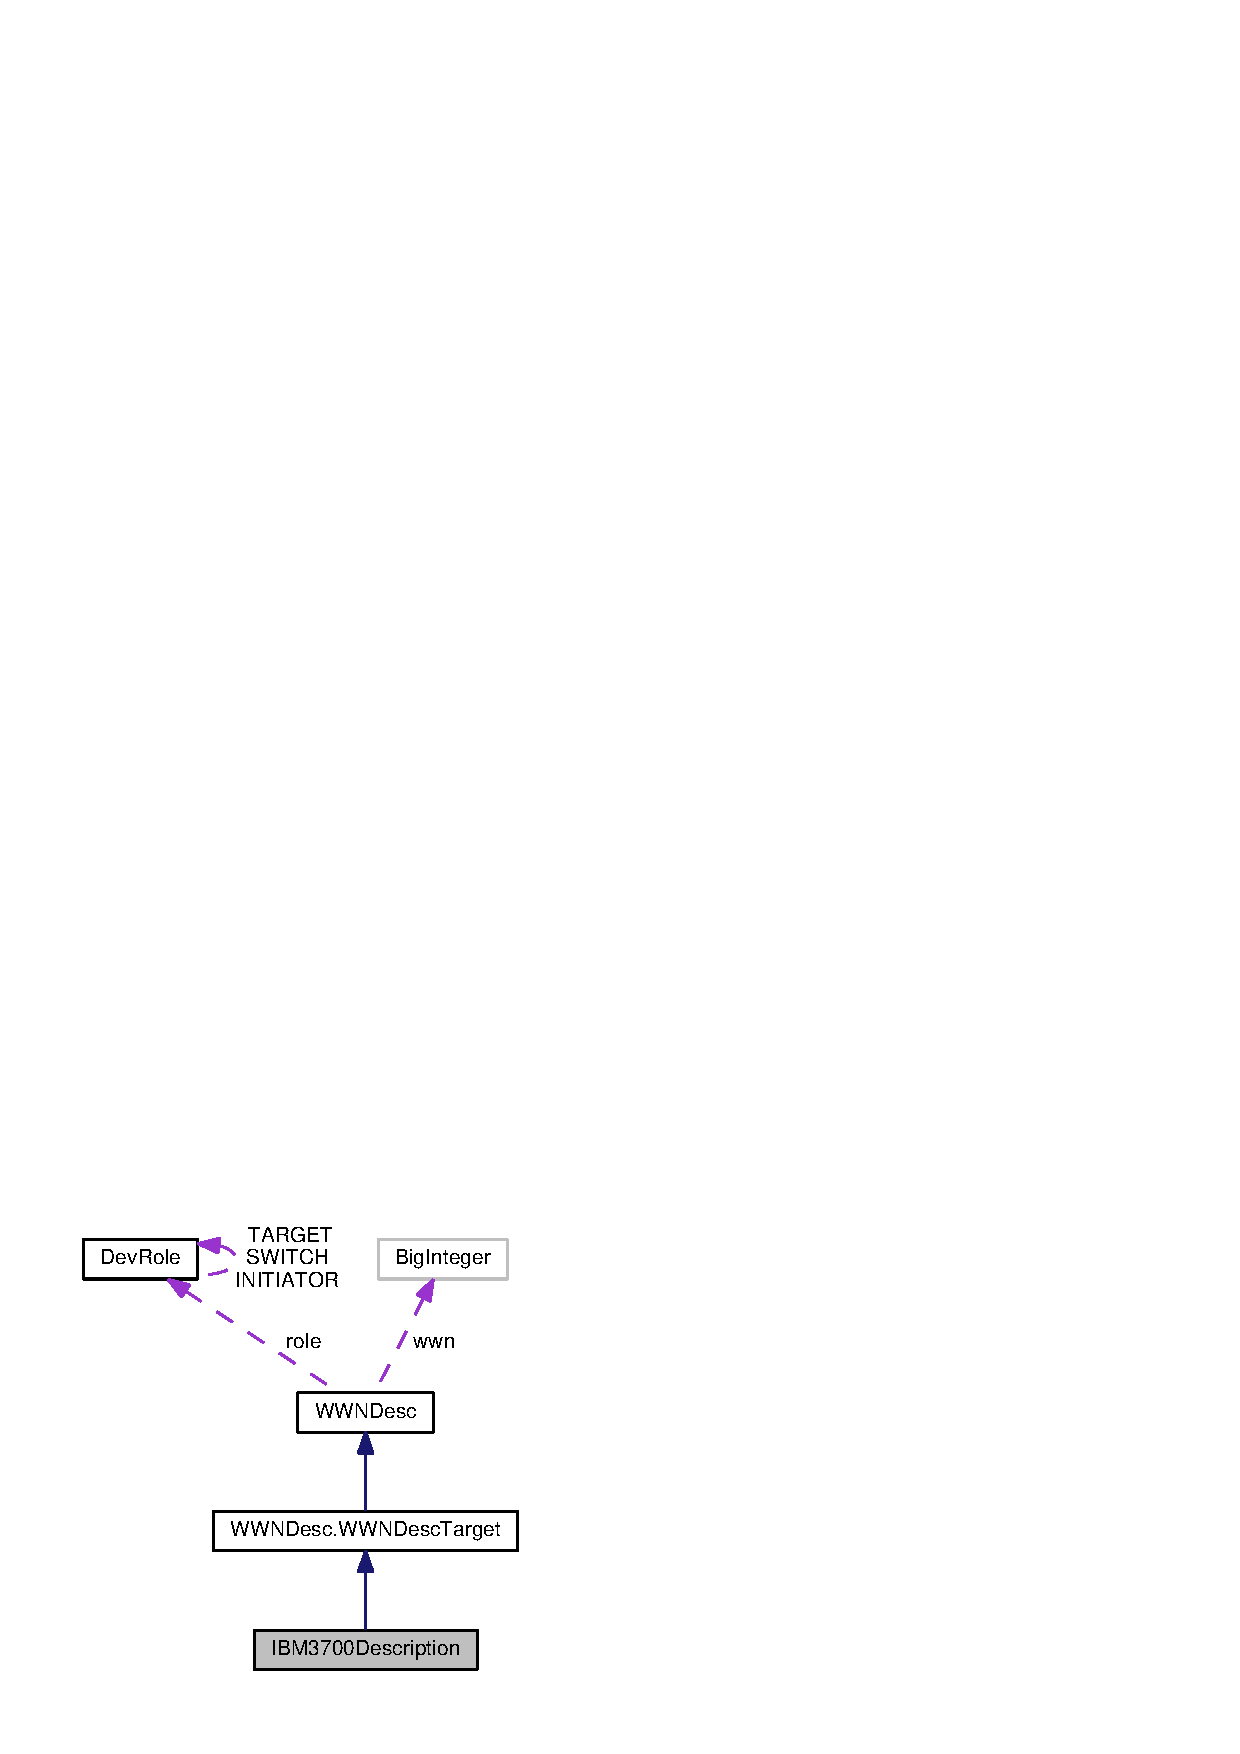
\includegraphics[width=249pt]{classorg_1_1smallfoot_1_1wwn_1_1IBM3700Description__coll__graph}
\end{center}
\end{figure}
\subsection*{Public Member Functions}
\begin{DoxyCompactItemize}
\item 
{\bf I\+B\+M3700\+Description} (String {\bf wwn})
\begin{DoxyCompactList}\small\item\em create an instance with \doxyref{brief}{p.}{classorg_1_1smallfoot_1_1wwn_1_1WWNDesc_adbebed411e8c47d43338efa3edaa13f8} set to false. \end{DoxyCompactList}\item 
{\bf I\+B\+M3700\+Description} (boolean {\bf brief}, String {\bf wwn})
\begin{DoxyCompactList}\small\item\em create an instance with the given W\+W\+N. \end{DoxyCompactList}\item 
String {\bf to\+String} ()
\begin{DoxyCompactList}\small\item\em return a description or alias for this W\+W\+N \end{DoxyCompactList}\end{DoxyCompactItemize}
\subsection*{Static Public Member Functions}
\begin{DoxyCompactItemize}
\item 
static {\bf W\+W\+N\+Desc} {\bf get\+Desc} (boolean strong, boolean {\bf brief}, String {\bf wwn})
\begin{DoxyCompactList}\small\item\em If this class matches or describes the given W\+W\+N, returns a new instance of this class loaded with the given W\+W\+N. \end{DoxyCompactList}\item 
static {\bf W\+W\+N\+Desc} {\bf get\+Desc} (boolean strong, boolean {\bf brief}, String {\bf wwn}, int {\bf role})
\begin{DoxyCompactList}\small\item\em If this class matches or describes the given W\+W\+N, returns a new instance of this class loaded with the given W\+W\+N. \end{DoxyCompactList}\end{DoxyCompactItemize}
\subsection*{Additional Inherited Members}


\subsection{Detailed Description}
\doxyref{I\+B\+M3700\+Description}{p.}{classorg_1_1smallfoot_1_1wwn_1_1IBM3700Description} (ie Ram\+San-\/\+G8332-\/\+F\+C-\/2\+B) breaks out the serial and port information from the Texas Memory Systems hardware initially called Ram\+San. 

Definition at line 13 of file I\+B\+M3700\+Description.\+java.



\subsection{Constructor \& Destructor Documentation}
\index{org\+::smallfoot\+::wwn\+::\+I\+B\+M3700\+Description@{org\+::smallfoot\+::wwn\+::\+I\+B\+M3700\+Description}!I\+B\+M3700\+Description@{I\+B\+M3700\+Description}}
\index{I\+B\+M3700\+Description@{I\+B\+M3700\+Description}!org\+::smallfoot\+::wwn\+::\+I\+B\+M3700\+Description@{org\+::smallfoot\+::wwn\+::\+I\+B\+M3700\+Description}}
\subsubsection[{I\+B\+M3700\+Description}]{\setlength{\rightskip}{0pt plus 5cm}{\bf I\+B\+M3700\+Description} (
\begin{DoxyParamCaption}
\item[{String}]{wwn}
\end{DoxyParamCaption}
)\hspace{0.3cm}{\ttfamily [inline]}}\label{classorg_1_1smallfoot_1_1wwn_1_1IBM3700Description_a956b2c06b0e4934236fcb08fba5807dd}


create an instance with \doxyref{brief}{p.}{classorg_1_1smallfoot_1_1wwn_1_1WWNDesc_adbebed411e8c47d43338efa3edaa13f8} set to false. 

This is a convenience function to support the older constructor model


\begin{DoxyExceptions}{Exceptions}
{\em java.\+lang.\+Null\+Pointer\+Exception} & if the given wwn is null\\
\hline
\end{DoxyExceptions}

\begin{DoxyParams}{Parameters}
{\em wwn} & the W\+W\+N to evaluate and describe \\
\hline
\end{DoxyParams}


Definition at line 16 of file I\+B\+M3700\+Description.\+java.



Referenced by I\+B\+M3700\+Description.\+get\+Desc().

\index{org\+::smallfoot\+::wwn\+::\+I\+B\+M3700\+Description@{org\+::smallfoot\+::wwn\+::\+I\+B\+M3700\+Description}!I\+B\+M3700\+Description@{I\+B\+M3700\+Description}}
\index{I\+B\+M3700\+Description@{I\+B\+M3700\+Description}!org\+::smallfoot\+::wwn\+::\+I\+B\+M3700\+Description@{org\+::smallfoot\+::wwn\+::\+I\+B\+M3700\+Description}}
\subsubsection[{I\+B\+M3700\+Description}]{\setlength{\rightskip}{0pt plus 5cm}{\bf I\+B\+M3700\+Description} (
\begin{DoxyParamCaption}
\item[{boolean}]{brief, }
\item[{String}]{wwn}
\end{DoxyParamCaption}
)\hspace{0.3cm}{\ttfamily [inline]}}\label{classorg_1_1smallfoot_1_1wwn_1_1IBM3700Description_ae6037d4ae31df18dbdc9a4e09f85e8a8}


create an instance with the given W\+W\+N. 

Values given to the constructor are simply copied to internal variables for later use


\begin{DoxyExceptions}{Exceptions}
{\em java.\+lang.\+Null\+Pointer\+Exception} & if the given wwn is null\\
\hline
\end{DoxyExceptions}

\begin{DoxyParams}{Parameters}
{\em brief} & whether an abbreviated description is requested \\
\hline
{\em wwn} & the W\+W\+N to evaluate and describe \\
\hline
\end{DoxyParams}


Definition at line 21 of file I\+B\+M3700\+Description.\+java.



\subsection{Member Function Documentation}
\index{org\+::smallfoot\+::wwn\+::\+I\+B\+M3700\+Description@{org\+::smallfoot\+::wwn\+::\+I\+B\+M3700\+Description}!get\+Desc@{get\+Desc}}
\index{get\+Desc@{get\+Desc}!org\+::smallfoot\+::wwn\+::\+I\+B\+M3700\+Description@{org\+::smallfoot\+::wwn\+::\+I\+B\+M3700\+Description}}
\subsubsection[{get\+Desc}]{\setlength{\rightskip}{0pt plus 5cm}static {\bf W\+W\+N\+Desc} get\+Desc (
\begin{DoxyParamCaption}
\item[{boolean}]{strong, }
\item[{boolean}]{brief, }
\item[{String}]{wwn}
\end{DoxyParamCaption}
)\hspace{0.3cm}{\ttfamily [inline]}, {\ttfamily [static]}}\label{classorg_1_1smallfoot_1_1wwn_1_1IBM3700Description_a7e34be4d9bd11a9971c007c6231b8c01}


If this class matches or describes the given W\+W\+N, returns a new instance of this class loaded with the given W\+W\+N. 

\begin{DoxyReturn}{Returns}
new instance of this class, or null if the given wwn does not match this class 
\end{DoxyReturn}

\begin{DoxyParams}{Parameters}
{\em strong} & is ignored\+: this class is a strong representation, not a weak one based on empirical matching, hence can always be used with confidence \\
\hline
{\em brief} & is ignored\+: this class has only one representation of the W\+W\+N description or alias \\
\hline
{\em wwn} & the W\+W\+N (W\+W\+P\+N or W\+W\+N\+N, but typically W\+W\+P\+N) to match \\
\hline
\end{DoxyParams}


Definition at line 34 of file I\+B\+M3700\+Description.\+java.



References Dev\+Role.\+max.



Referenced by W\+W\+N\+Description.\+get\+W\+W\+N\+Descriptor().

\index{org\+::smallfoot\+::wwn\+::\+I\+B\+M3700\+Description@{org\+::smallfoot\+::wwn\+::\+I\+B\+M3700\+Description}!get\+Desc@{get\+Desc}}
\index{get\+Desc@{get\+Desc}!org\+::smallfoot\+::wwn\+::\+I\+B\+M3700\+Description@{org\+::smallfoot\+::wwn\+::\+I\+B\+M3700\+Description}}
\subsubsection[{get\+Desc}]{\setlength{\rightskip}{0pt plus 5cm}static {\bf W\+W\+N\+Desc} get\+Desc (
\begin{DoxyParamCaption}
\item[{boolean}]{strong, }
\item[{boolean}]{brief, }
\item[{String}]{wwn, }
\item[{int}]{role}
\end{DoxyParamCaption}
)\hspace{0.3cm}{\ttfamily [inline]}, {\ttfamily [static]}}\label{classorg_1_1smallfoot_1_1wwn_1_1IBM3700Description_a37ac294533314b3b7b3a5f3404ee43d6}


If this class matches or describes the given W\+W\+N, returns a new instance of this class loaded with the given W\+W\+N. 

\begin{DoxyReturn}{Returns}
new instance of this class, or null if the given wwn does not match this class 
\end{DoxyReturn}

\begin{DoxyParams}{Parameters}
{\em strong} & is ignored\+: this class is a strong representation, not a weak one based on empirical matching, hence can always be used with confidence \\
\hline
{\em brief} & is ignored\+: this class has only one representation of the W\+W\+N description or alias \\
\hline
{\em wwn} & the W\+W\+N (W\+W\+P\+N or W\+W\+N\+N, but typically W\+W\+P\+N) to match \\
\hline
{\em role} & Role (Initiator/\+Switch/\+Target) to check for \\
\hline
\end{DoxyParams}


Definition at line 42 of file I\+B\+M3700\+Description.\+java.



References I\+B\+M3700\+Description.\+I\+B\+M3700\+Description(), and W\+W\+N\+Desc.\+W\+W\+N\+Desc\+Target.\+is\+A().



Here is the call graph for this function\+:\nopagebreak
\begin{figure}[H]
\begin{center}
\leavevmode
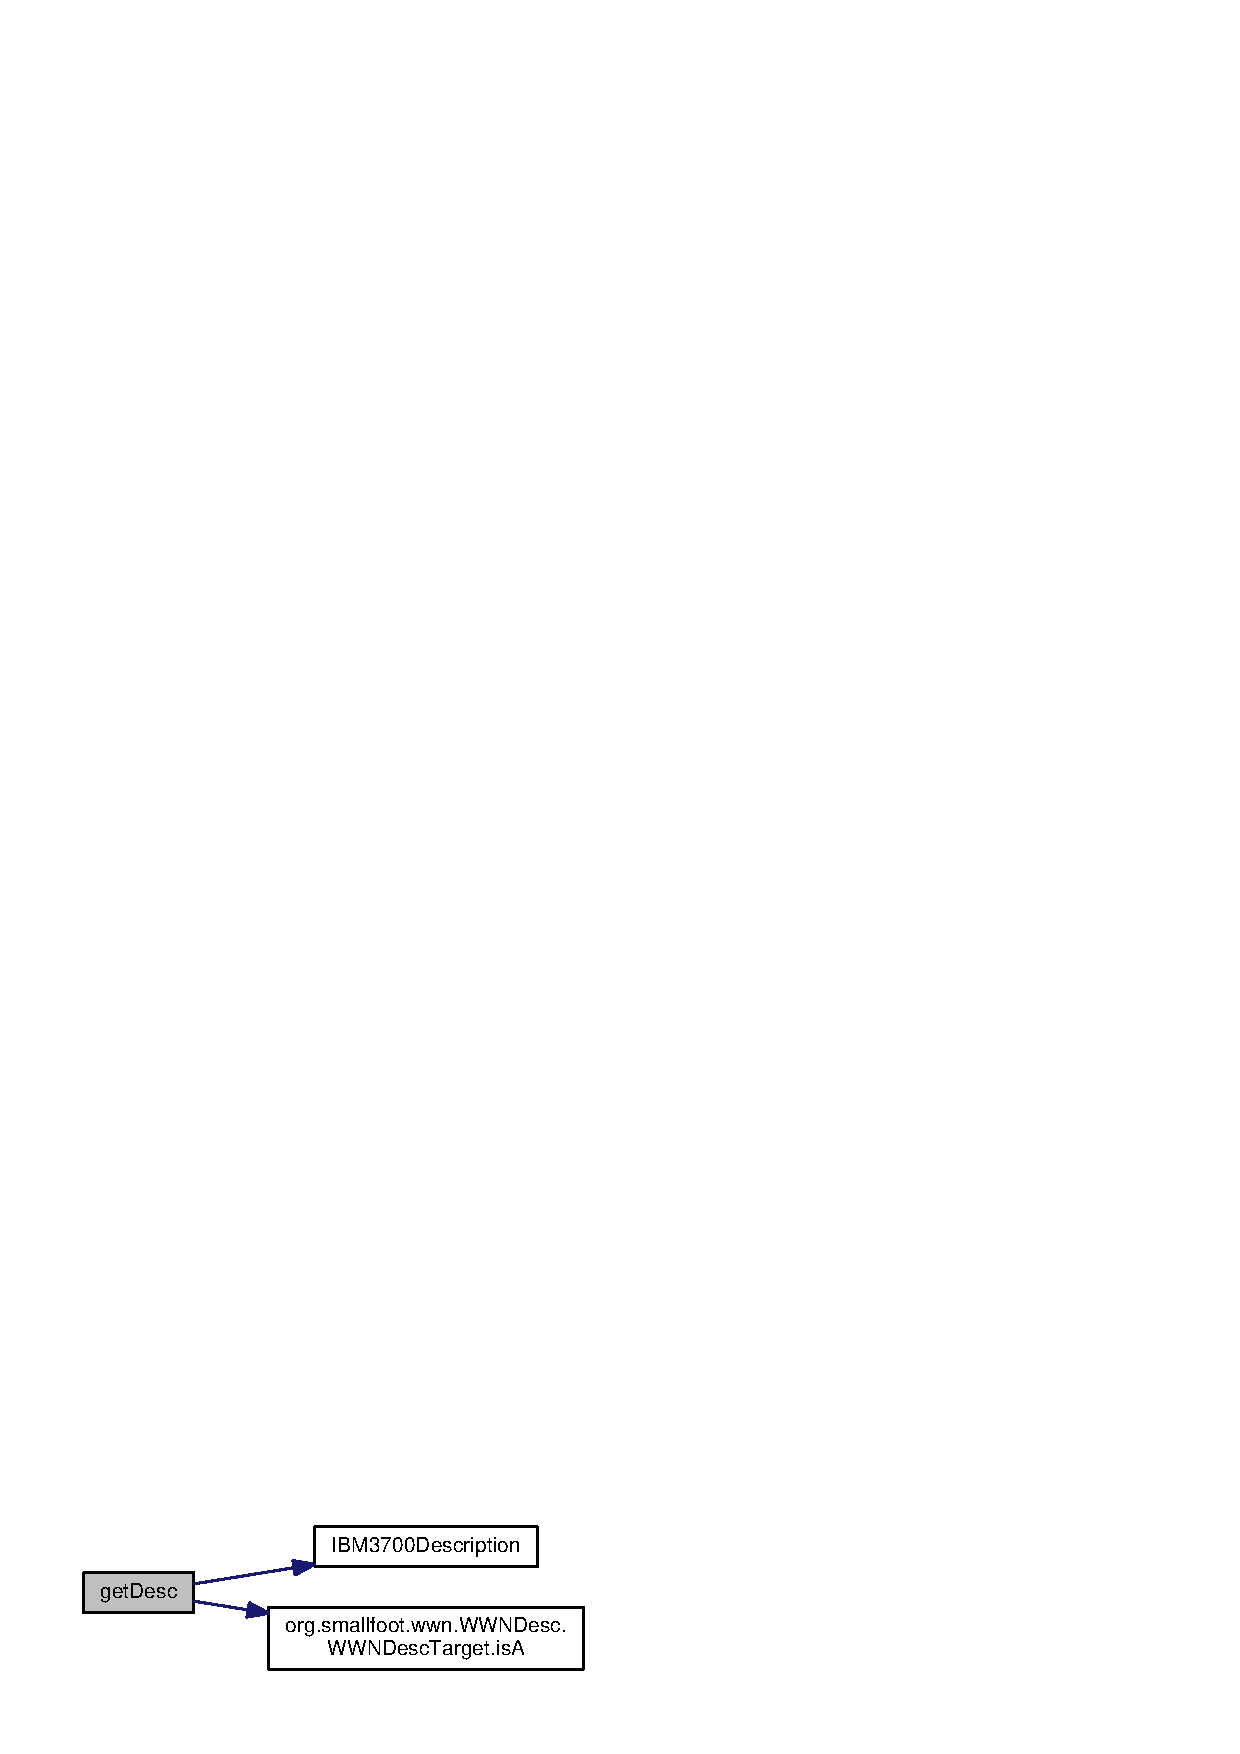
\includegraphics[width=284pt]{classorg_1_1smallfoot_1_1wwn_1_1IBM3700Description_a37ac294533314b3b7b3a5f3404ee43d6_cgraph}
\end{center}
\end{figure}


\index{org\+::smallfoot\+::wwn\+::\+I\+B\+M3700\+Description@{org\+::smallfoot\+::wwn\+::\+I\+B\+M3700\+Description}!to\+String@{to\+String}}
\index{to\+String@{to\+String}!org\+::smallfoot\+::wwn\+::\+I\+B\+M3700\+Description@{org\+::smallfoot\+::wwn\+::\+I\+B\+M3700\+Description}}
\subsubsection[{to\+String}]{\setlength{\rightskip}{0pt plus 5cm}String to\+String (
\begin{DoxyParamCaption}
{}
\end{DoxyParamCaption}
)\hspace{0.3cm}{\ttfamily [inline]}}\label{classorg_1_1smallfoot_1_1wwn_1_1IBM3700Description_ad146fa8579a5f8a876c4688cc5a68520}


return a description or alias for this W\+W\+N 

\begin{DoxyReturn}{Returns}
generated alias or nickname for the W\+W\+N 
\end{DoxyReturn}


Definition at line 57 of file I\+B\+M3700\+Description.\+java.



References W\+W\+N\+Desc.\+wwn.



The documentation for this class was generated from the following file\+:\begin{DoxyCompactItemize}
\item 
java/{\bf I\+B\+M3700\+Description.\+java}\end{DoxyCompactItemize}

\section{I\-B\-M\-S\-V\-C\-Description Class Reference}
\label{classorg_1_1smallfoot_1_1wwn_1_1IBMSVCDescription}\index{I\-B\-M\-S\-V\-C\-Description@{I\-B\-M\-S\-V\-C\-Description}}


Inheritance diagram for I\-B\-M\-S\-V\-C\-Description\-:\nopagebreak
\begin{figure}[H]
\begin{center}
\leavevmode
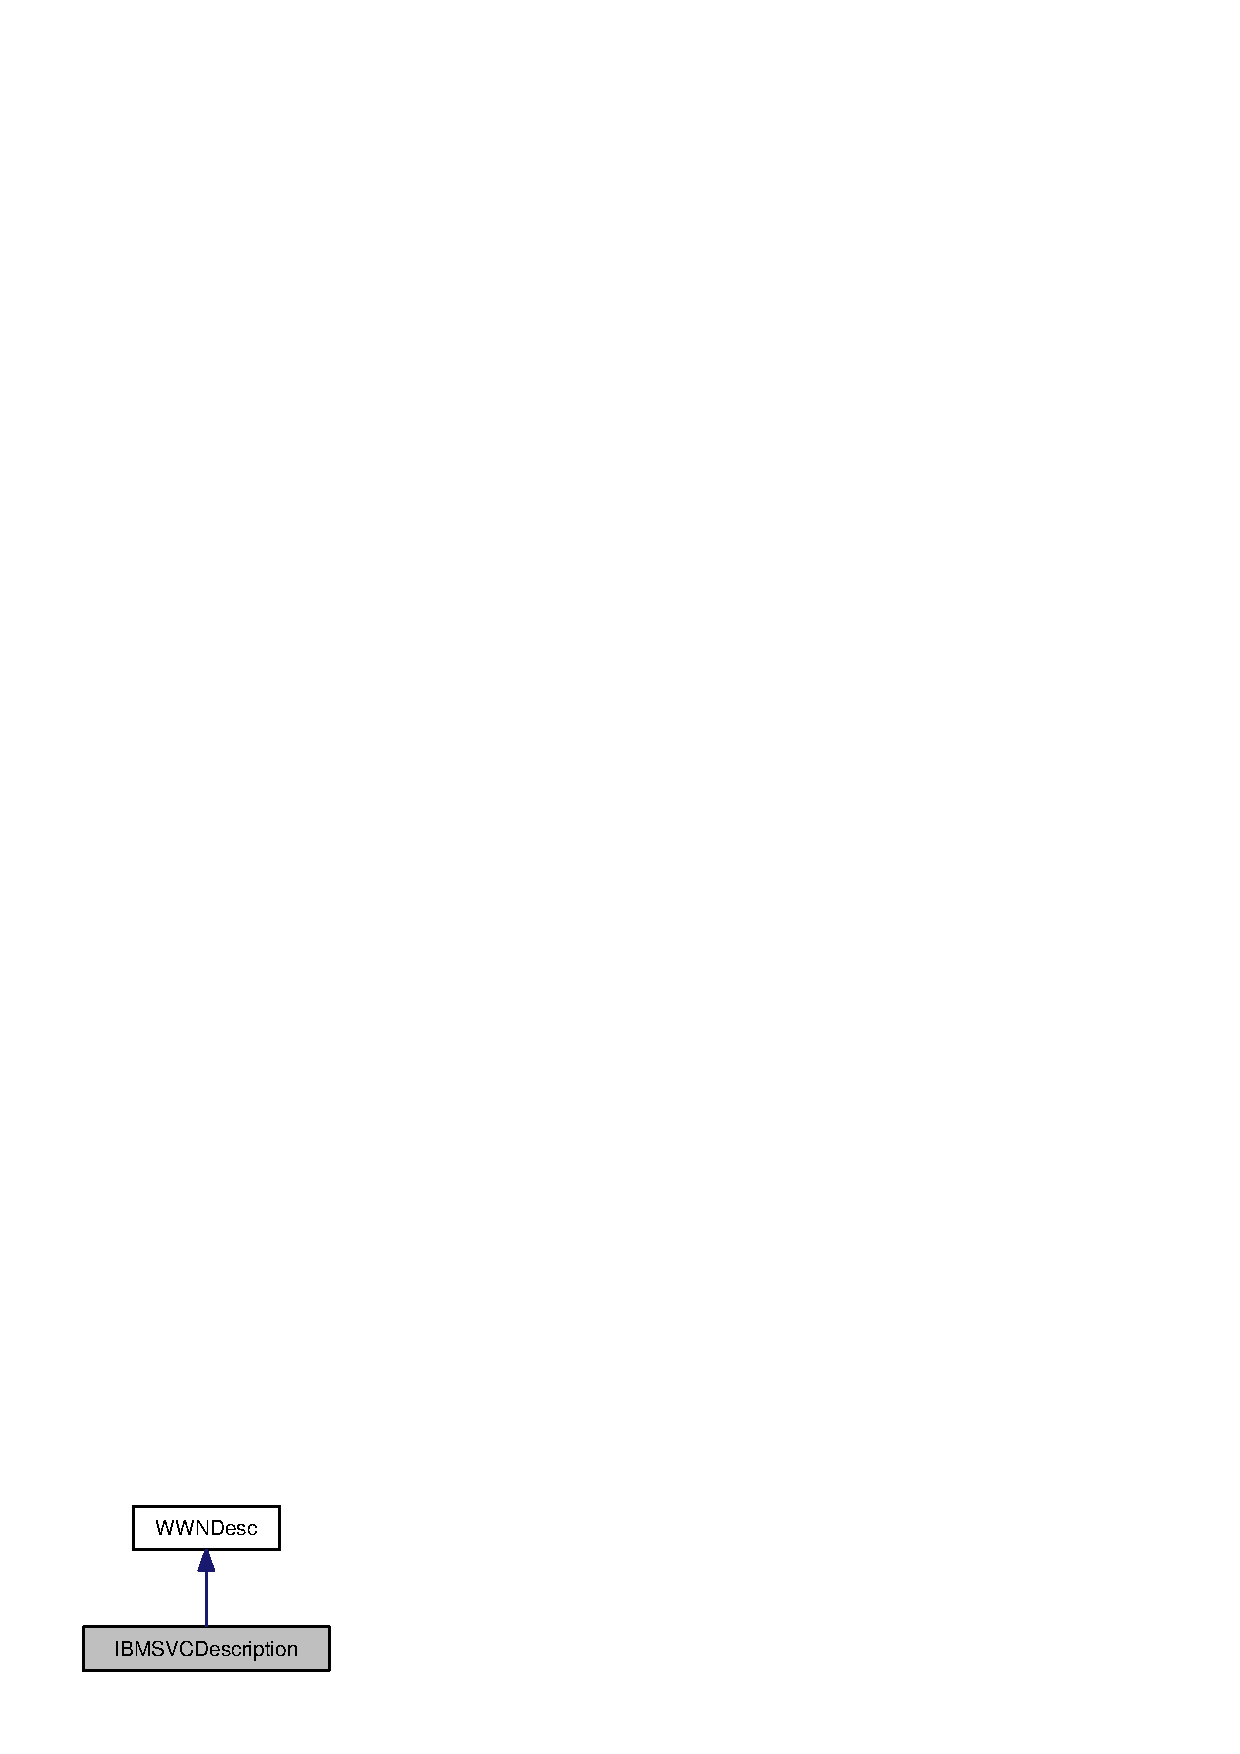
\includegraphics[width=162pt]{classorg_1_1smallfoot_1_1wwn_1_1IBMSVCDescription__inherit__graph}
\end{center}
\end{figure}


Collaboration diagram for I\-B\-M\-S\-V\-C\-Description\-:\nopagebreak
\begin{figure}[H]
\begin{center}
\leavevmode
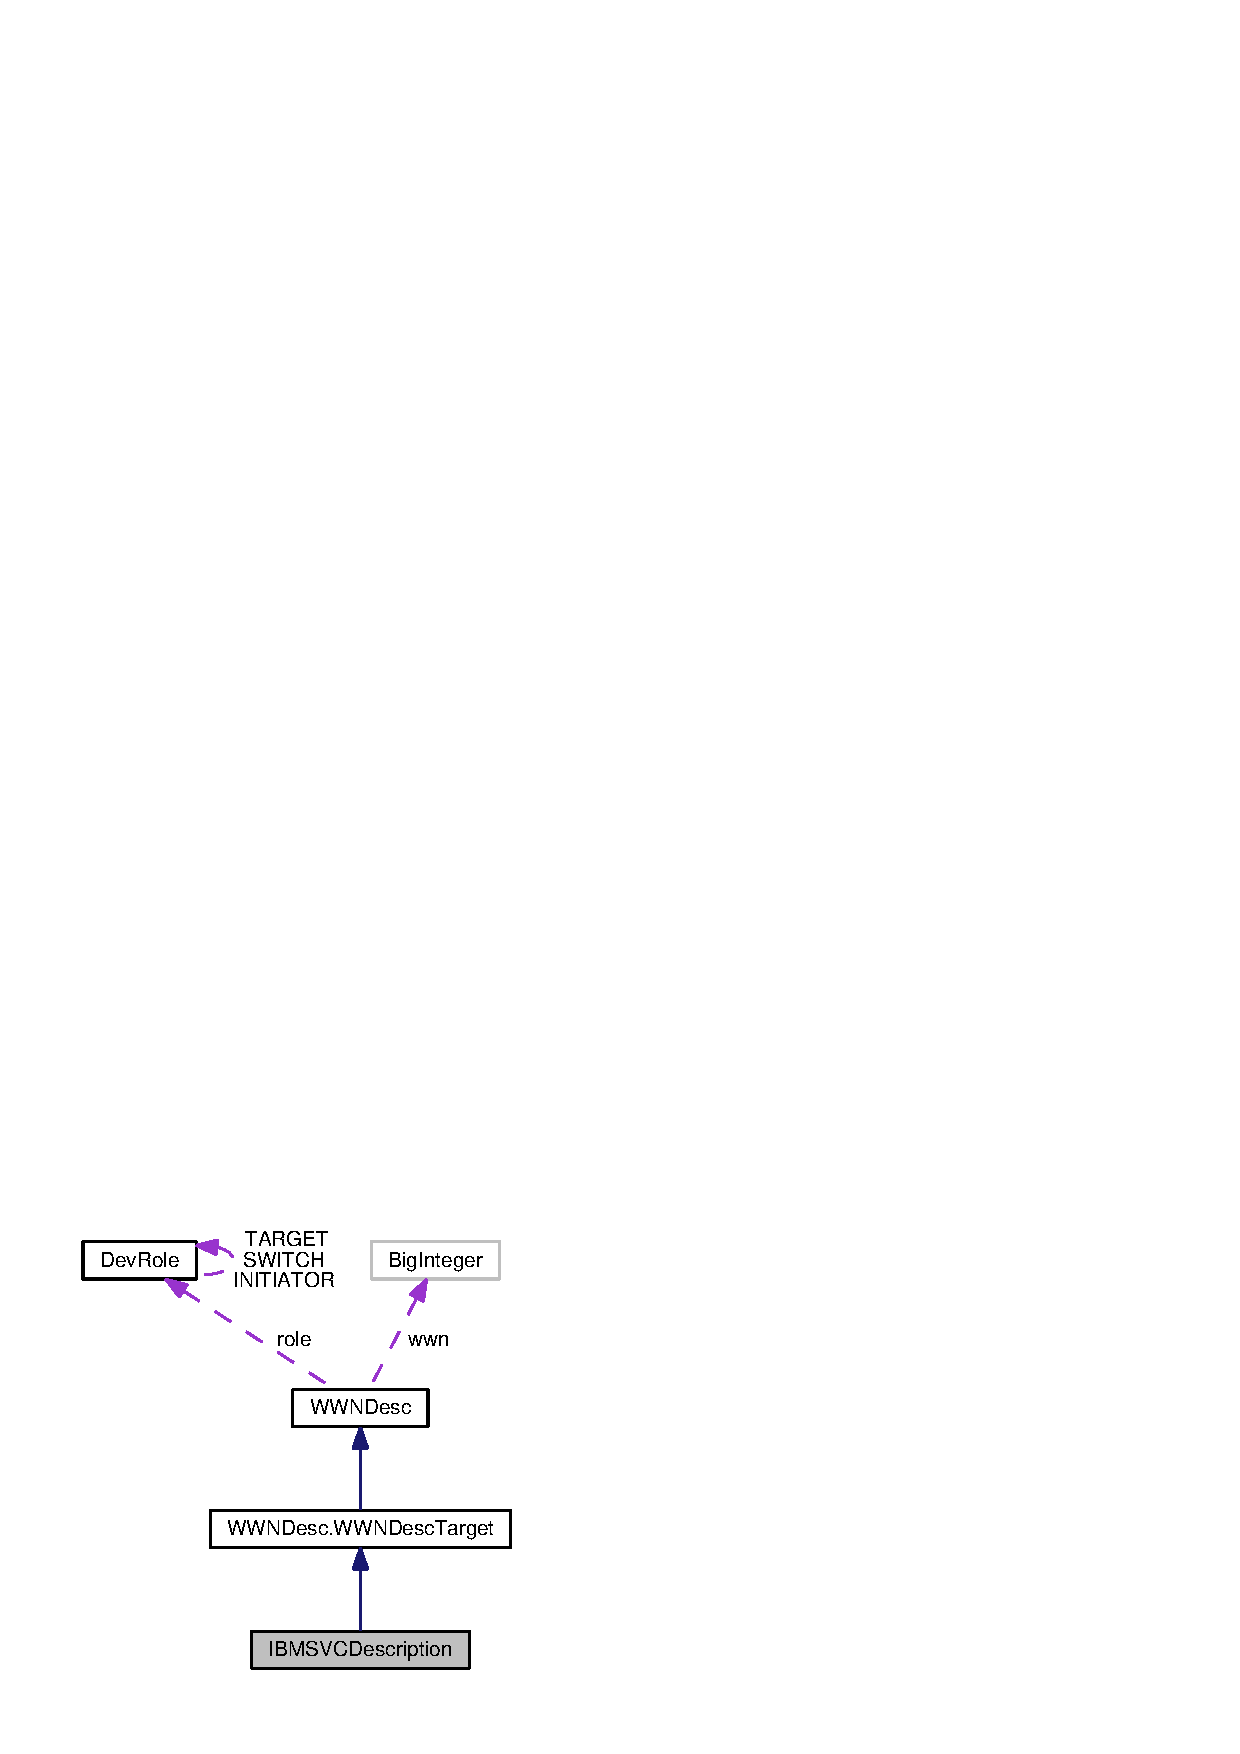
\includegraphics[width=162pt]{classorg_1_1smallfoot_1_1wwn_1_1IBMSVCDescription__coll__graph}
\end{center}
\end{figure}
\subsection*{Public Member Functions}
\begin{DoxyCompactItemize}
\item 
{\bf I\-B\-M\-S\-V\-C\-Description} (String wwn)
\begin{DoxyCompactList}\small\item\em create an instance with this.\-brief set to false. \end{DoxyCompactList}\item 
{\bf I\-B\-M\-S\-V\-C\-Description} (boolean brief, String wwn)
\begin{DoxyCompactList}\small\item\em create an instance with the given W\-W\-N. \end{DoxyCompactList}\item 
String {\bf to\-String} ()
\begin{DoxyCompactList}\small\item\em return a description or alias for this W\-W\-N; if brief is set to true during the call to \doxyref{get\-Desc()}{p.}{classorg_1_1smallfoot_1_1wwn_1_1IBMSVCDescription_a7e34be4d9bd11a9971c007c6231b8c01}, then a shorter description or alias will be returned \end{DoxyCompactList}\end{DoxyCompactItemize}
\subsection*{Static Public Member Functions}
\begin{DoxyCompactItemize}
\item 
static {\bf W\-W\-N\-Desc} {\bf get\-Desc} (boolean strong, boolean brief, String wwn)
\begin{DoxyCompactList}\small\item\em If this class matches or describes the given W\-W\-N, returns a new instance of this class loaded with the given W\-W\-N. \end{DoxyCompactList}\end{DoxyCompactItemize}


\subsection{Detailed Description}


Definition at line 10 of file I\-B\-M\-S\-V\-C\-Description.\-java.



\subsection{Constructor \& Destructor Documentation}
\index{org\-::smallfoot\-::wwn\-::\-I\-B\-M\-S\-V\-C\-Description@{org\-::smallfoot\-::wwn\-::\-I\-B\-M\-S\-V\-C\-Description}!I\-B\-M\-S\-V\-C\-Description@{I\-B\-M\-S\-V\-C\-Description}}
\index{I\-B\-M\-S\-V\-C\-Description@{I\-B\-M\-S\-V\-C\-Description}!org::smallfoot::wwn::IBMSVCDescription@{org\-::smallfoot\-::wwn\-::\-I\-B\-M\-S\-V\-C\-Description}}
\subsubsection[{I\-B\-M\-S\-V\-C\-Description}]{\setlength{\rightskip}{0pt plus 5cm}{\bf I\-B\-M\-S\-V\-C\-Description} (
\begin{DoxyParamCaption}
\item[{String}]{wwn}
\end{DoxyParamCaption}
)\hspace{0.3cm}{\ttfamily [inline]}}\label{classorg_1_1smallfoot_1_1wwn_1_1IBMSVCDescription_a57a4e0da6d730a8b79fa3deabf6e59dd}


create an instance with this.\-brief set to false. 

This is a convenience function to support the older constructor model


\begin{DoxyParams}{Parameters}
{\em wwn} & the W\-W\-N to evaluate and describe \\
\hline
\end{DoxyParams}


Definition at line 13 of file I\-B\-M\-S\-V\-C\-Description.\-java.



Referenced by I\-B\-M\-S\-V\-C\-Description.\-get\-Desc().

\index{org\-::smallfoot\-::wwn\-::\-I\-B\-M\-S\-V\-C\-Description@{org\-::smallfoot\-::wwn\-::\-I\-B\-M\-S\-V\-C\-Description}!I\-B\-M\-S\-V\-C\-Description@{I\-B\-M\-S\-V\-C\-Description}}
\index{I\-B\-M\-S\-V\-C\-Description@{I\-B\-M\-S\-V\-C\-Description}!org::smallfoot::wwn::IBMSVCDescription@{org\-::smallfoot\-::wwn\-::\-I\-B\-M\-S\-V\-C\-Description}}
\subsubsection[{I\-B\-M\-S\-V\-C\-Description}]{\setlength{\rightskip}{0pt plus 5cm}{\bf I\-B\-M\-S\-V\-C\-Description} (
\begin{DoxyParamCaption}
\item[{boolean}]{brief, }
\item[{String}]{wwn}
\end{DoxyParamCaption}
)\hspace{0.3cm}{\ttfamily [inline]}}\label{classorg_1_1smallfoot_1_1wwn_1_1IBMSVCDescription_a063df7534db1b95a74bfe2e5e84c1331}


create an instance with the given W\-W\-N. 

Values given to the constructor are simply copied to internal variables for later use


\begin{DoxyParams}{Parameters}
{\em brief} & whether an abbreviated description is requested \\
\hline
{\em wwn} & the W\-W\-N to evaluate and describe \\
\hline
\end{DoxyParams}


Definition at line 18 of file I\-B\-M\-S\-V\-C\-Description.\-java.



\subsection{Member Function Documentation}
\index{org\-::smallfoot\-::wwn\-::\-I\-B\-M\-S\-V\-C\-Description@{org\-::smallfoot\-::wwn\-::\-I\-B\-M\-S\-V\-C\-Description}!get\-Desc@{get\-Desc}}
\index{get\-Desc@{get\-Desc}!org::smallfoot::wwn::IBMSVCDescription@{org\-::smallfoot\-::wwn\-::\-I\-B\-M\-S\-V\-C\-Description}}
\subsubsection[{get\-Desc}]{\setlength{\rightskip}{0pt plus 5cm}static {\bf W\-W\-N\-Desc} get\-Desc (
\begin{DoxyParamCaption}
\item[{boolean}]{strong, }
\item[{boolean}]{brief, }
\item[{String}]{wwn}
\end{DoxyParamCaption}
)\hspace{0.3cm}{\ttfamily [inline]}, {\ttfamily [static]}}\label{classorg_1_1smallfoot_1_1wwn_1_1IBMSVCDescription_a7e34be4d9bd11a9971c007c6231b8c01}


If this class matches or describes the given W\-W\-N, returns a new instance of this class loaded with the given W\-W\-N. 

\begin{DoxyReturn}{Returns}
new instance of this class, or null if the given wwn does not match this class 
\end{DoxyReturn}

\begin{DoxyParams}{Parameters}
{\em strong} & is ignored\-: this class is a strong representation, not a weak one based on empirical matching, hence can always be used with confidence \\
\hline
{\em brief} & is used to ask for a shorter description\-: a more concise nickname or alias \\
\hline
{\em wwn} & the W\-W\-N (W\-W\-P\-N or W\-W\-N\-N, but typically W\-W\-P\-N) to match \\
\hline
\end{DoxyParams}


Definition at line 31 of file I\-B\-M\-S\-V\-C\-Description.\-java.



References I\-B\-M\-S\-V\-C\-Description.\-I\-B\-M\-S\-V\-C\-Description().



Referenced by W\-W\-N\-Description.\-get\-W\-W\-N\-Descriptor().



Here is the call graph for this function\-:\nopagebreak
\begin{figure}[H]
\begin{center}
\leavevmode
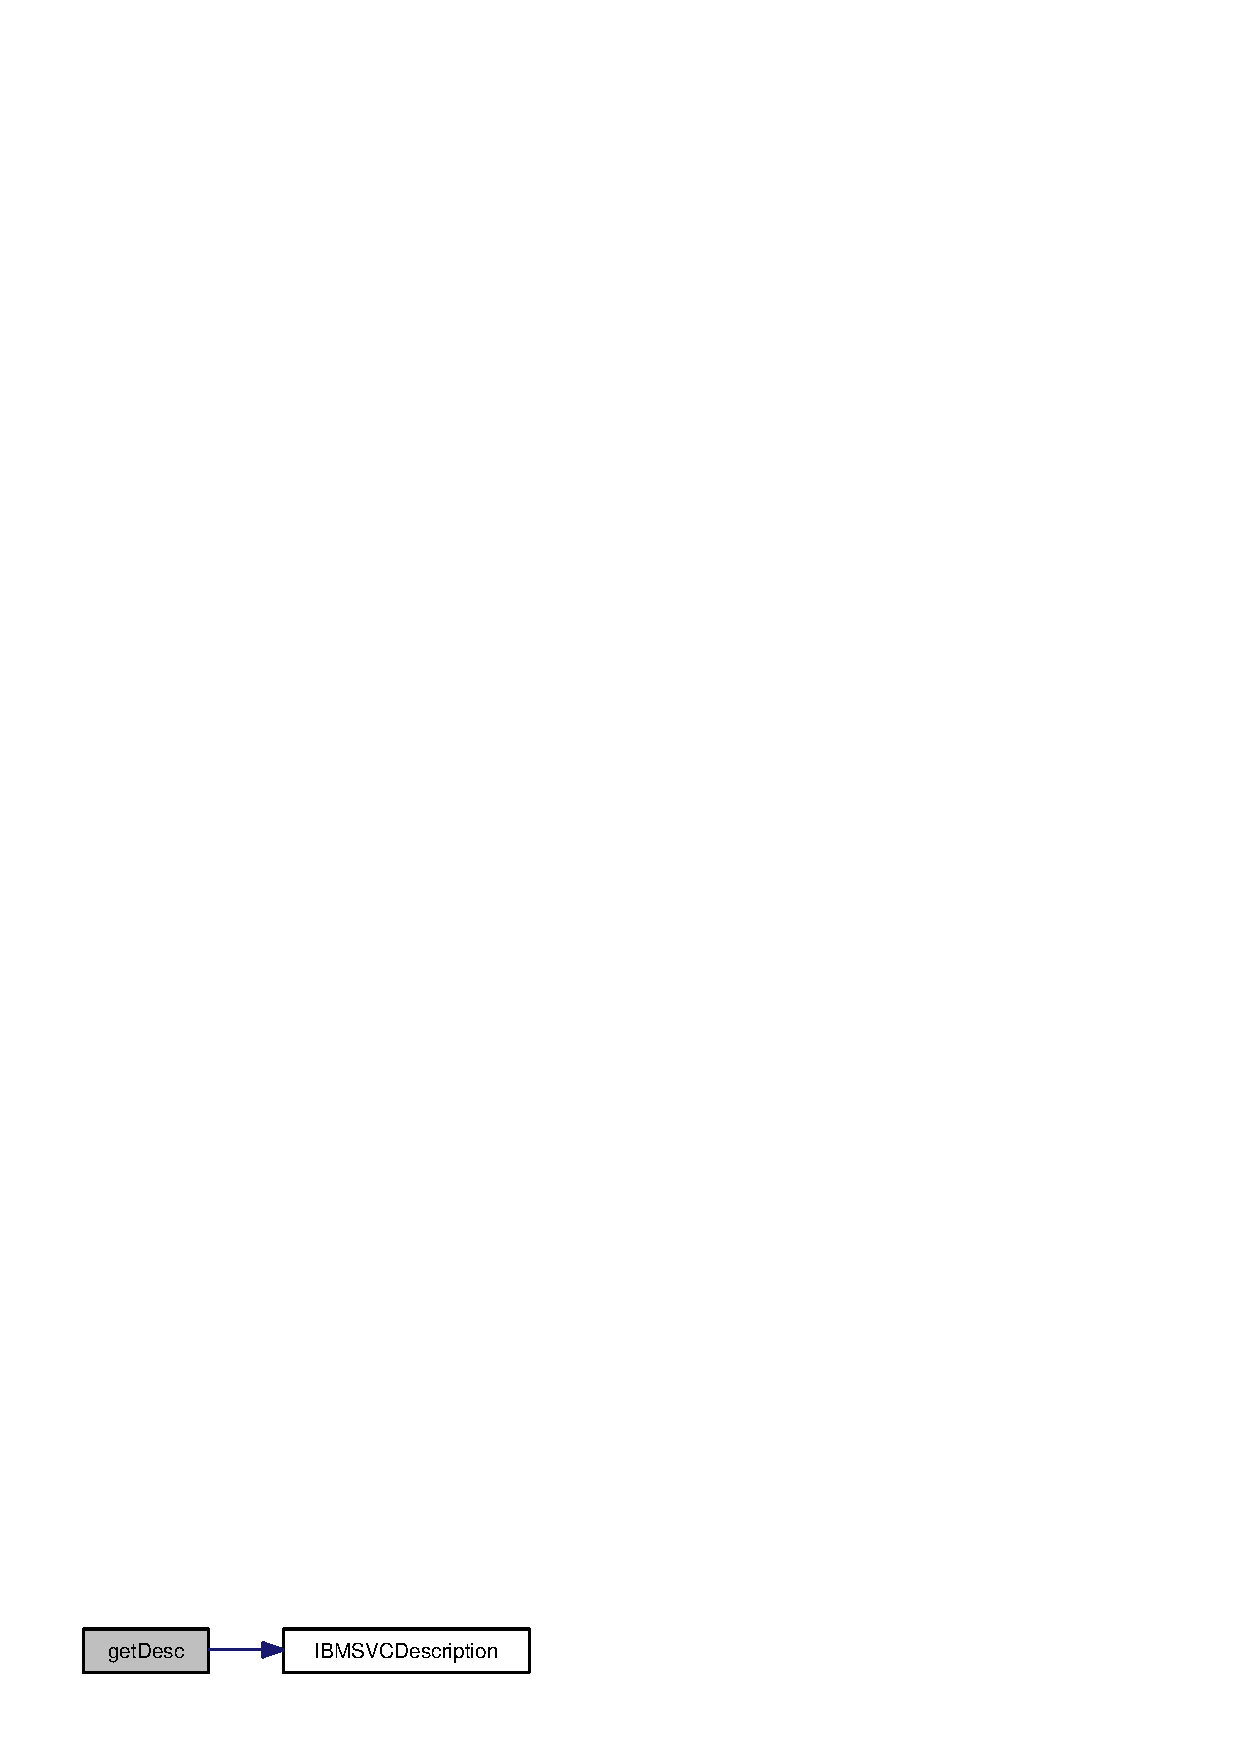
\includegraphics[width=258pt]{classorg_1_1smallfoot_1_1wwn_1_1IBMSVCDescription_a7e34be4d9bd11a9971c007c6231b8c01_cgraph}
\end{center}
\end{figure}


\index{org\-::smallfoot\-::wwn\-::\-I\-B\-M\-S\-V\-C\-Description@{org\-::smallfoot\-::wwn\-::\-I\-B\-M\-S\-V\-C\-Description}!to\-String@{to\-String}}
\index{to\-String@{to\-String}!org::smallfoot::wwn::IBMSVCDescription@{org\-::smallfoot\-::wwn\-::\-I\-B\-M\-S\-V\-C\-Description}}
\subsubsection[{to\-String}]{\setlength{\rightskip}{0pt plus 5cm}String to\-String (
\begin{DoxyParamCaption}
{}
\end{DoxyParamCaption}
)\hspace{0.3cm}{\ttfamily [inline]}}\label{classorg_1_1smallfoot_1_1wwn_1_1IBMSVCDescription_ad146fa8579a5f8a876c4688cc5a68520}


return a description or alias for this W\-W\-N; if brief is set to true during the call to \doxyref{get\-Desc()}{p.}{classorg_1_1smallfoot_1_1wwn_1_1IBMSVCDescription_a7e34be4d9bd11a9971c007c6231b8c01}, then a shorter description or alias will be returned 

\begin{DoxySeeAlso}{See Also}
\doxyref{get\-Desc(boolean,boolean,\-String)}{p.}{classorg_1_1smallfoot_1_1wwn_1_1IBMSVCDescription_a7e34be4d9bd11a9971c007c6231b8c01}
\end{DoxySeeAlso}
\begin{DoxyReturn}{Returns}
generated alias or nickname for the W\-W\-N 
\end{DoxyReturn}


Definition at line 46 of file I\-B\-M\-S\-V\-C\-Description.\-java.



The documentation for this class was generated from the following file\-:\begin{DoxyCompactItemize}
\item 
java/{\bf I\-B\-M\-S\-V\-C\-Description.\-java}\end{DoxyCompactItemize}

\section{Net\-App\-Description Class Reference}
\label{classorg_1_1smallfoot_1_1wwn_1_1NetAppDescription}\index{Net\-App\-Description@{Net\-App\-Description}}


\doxyref{Net\-App\-Description}{p.}{classorg_1_1smallfoot_1_1wwn_1_1NetAppDescription} (ie Net\-App-\/123456-\/i\-Grp1-\/0a) breaks out the serial, I\-O Group, and port information from the W\-W\-P\-N.  




Inheritance diagram for Net\-App\-Description\-:\nopagebreak
\begin{figure}[H]
\begin{center}
\leavevmode
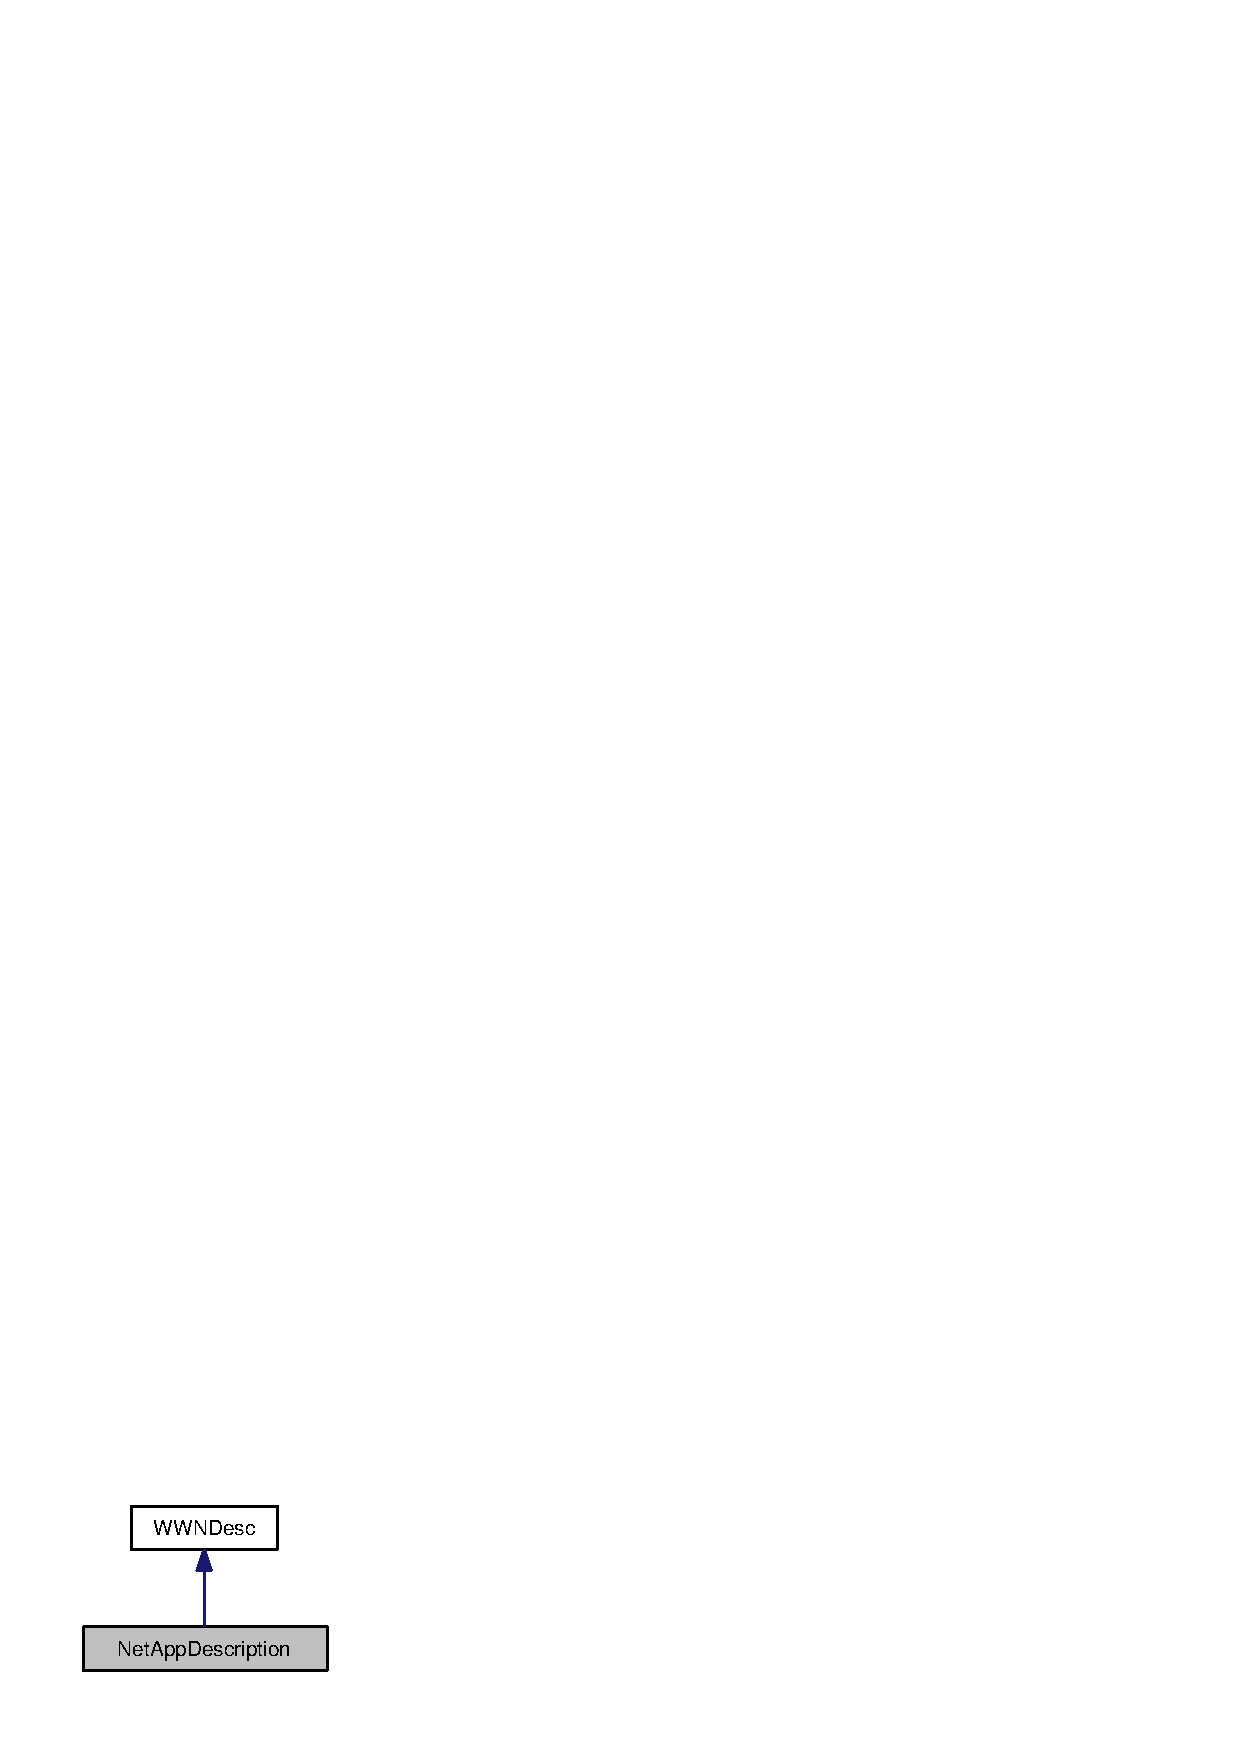
\includegraphics[width=160pt]{classorg_1_1smallfoot_1_1wwn_1_1NetAppDescription__inherit__graph}
\end{center}
\end{figure}


Collaboration diagram for Net\-App\-Description\-:\nopagebreak
\begin{figure}[H]
\begin{center}
\leavevmode
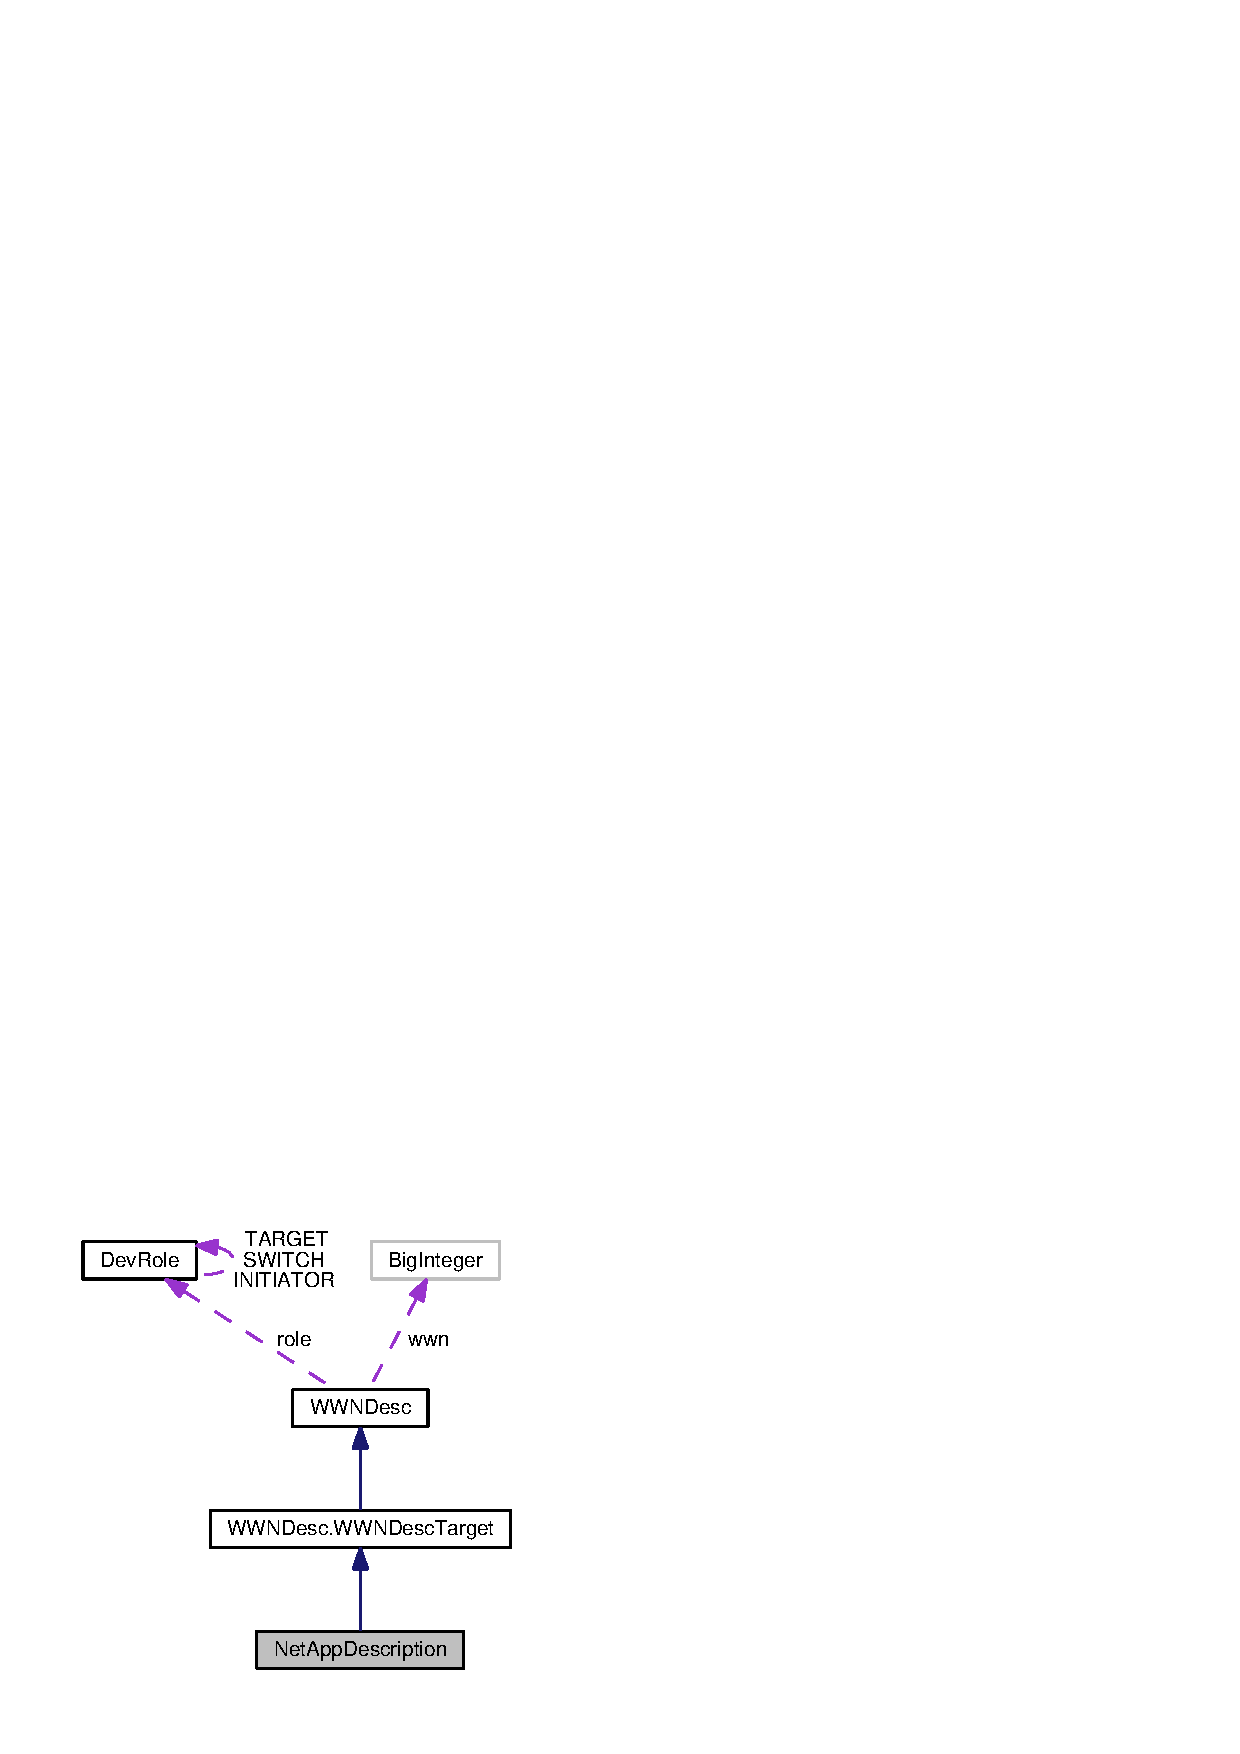
\includegraphics[width=160pt]{classorg_1_1smallfoot_1_1wwn_1_1NetAppDescription__coll__graph}
\end{center}
\end{figure}
\subsection*{Public Member Functions}
\begin{DoxyCompactItemize}
\item 
{\bf Net\-App\-Description} (String {\bf wwn})
\begin{DoxyCompactList}\small\item\em create an instance with \doxyref{brief}{p.}{classorg_1_1smallfoot_1_1wwn_1_1WWNDesc_adbebed411e8c47d43338efa3edaa13f8} set to false. \end{DoxyCompactList}\item 
{\bf Net\-App\-Description} (boolean {\bf brief}, String {\bf wwn})
\begin{DoxyCompactList}\small\item\em create an instance with the given W\-W\-N. \end{DoxyCompactList}\item 
String {\bf to\-String} ()
\begin{DoxyCompactList}\small\item\em return a description or alias for this W\-W\-N; if brief is set to true during the call to \doxyref{get\-Desc()}{p.}{classorg_1_1smallfoot_1_1wwn_1_1NetAppDescription_a7e34be4d9bd11a9971c007c6231b8c01}, then a shorter description or alias will be returned \end{DoxyCompactList}\end{DoxyCompactItemize}
\subsection*{Static Public Member Functions}
\begin{DoxyCompactItemize}
\item 
static {\bf W\-W\-N\-Desc} {\bf get\-Desc} (boolean strong, boolean {\bf brief}, String {\bf wwn})
\begin{DoxyCompactList}\small\item\em If this class matches or describes the given W\-W\-N, returns a new instance of this class loaded with the given W\-W\-N. \end{DoxyCompactList}\end{DoxyCompactItemize}
\subsection*{Additional Inherited Members}


\subsection{Detailed Description}
\doxyref{Net\-App\-Description}{p.}{classorg_1_1smallfoot_1_1wwn_1_1NetAppDescription} (ie Net\-App-\/123456-\/i\-Grp1-\/0a) breaks out the serial, I\-O Group, and port information from the W\-W\-P\-N. 

Definition at line 14 of file Net\-App\-Description.\-java.



\subsection{Constructor \& Destructor Documentation}
\index{org\-::smallfoot\-::wwn\-::\-Net\-App\-Description@{org\-::smallfoot\-::wwn\-::\-Net\-App\-Description}!Net\-App\-Description@{Net\-App\-Description}}
\index{Net\-App\-Description@{Net\-App\-Description}!org::smallfoot::wwn::NetAppDescription@{org\-::smallfoot\-::wwn\-::\-Net\-App\-Description}}
\subsubsection[{Net\-App\-Description}]{\setlength{\rightskip}{0pt plus 5cm}{\bf Net\-App\-Description} (
\begin{DoxyParamCaption}
\item[{String}]{wwn}
\end{DoxyParamCaption}
)\hspace{0.3cm}{\ttfamily [inline]}}\label{classorg_1_1smallfoot_1_1wwn_1_1NetAppDescription_ac528ef64391ea541bcb573fa7dd983a0}


create an instance with \doxyref{brief}{p.}{classorg_1_1smallfoot_1_1wwn_1_1WWNDesc_adbebed411e8c47d43338efa3edaa13f8} set to false. 

This is a convenience function to support the older constructor model


\begin{DoxyExceptions}{Exceptions}
{\em java.\-lang.\-Null\-Pointer\-Exception} & if the given wwn is null\\
\hline
\end{DoxyExceptions}

\begin{DoxyParams}{Parameters}
{\em wwn} & the W\-W\-N to evaluate and describe \\
\hline
\end{DoxyParams}


Definition at line 17 of file Net\-App\-Description.\-java.



Referenced by Net\-App\-Description.\-get\-Desc().

\index{org\-::smallfoot\-::wwn\-::\-Net\-App\-Description@{org\-::smallfoot\-::wwn\-::\-Net\-App\-Description}!Net\-App\-Description@{Net\-App\-Description}}
\index{Net\-App\-Description@{Net\-App\-Description}!org::smallfoot::wwn::NetAppDescription@{org\-::smallfoot\-::wwn\-::\-Net\-App\-Description}}
\subsubsection[{Net\-App\-Description}]{\setlength{\rightskip}{0pt plus 5cm}{\bf Net\-App\-Description} (
\begin{DoxyParamCaption}
\item[{boolean}]{brief, }
\item[{String}]{wwn}
\end{DoxyParamCaption}
)\hspace{0.3cm}{\ttfamily [inline]}}\label{classorg_1_1smallfoot_1_1wwn_1_1NetAppDescription_a11fdde1c8d9837b45468199530c747f4}


create an instance with the given W\-W\-N. 

Values given to the constructor are simply copied to internal variables for later use


\begin{DoxyExceptions}{Exceptions}
{\em java.\-lang.\-Null\-Pointer\-Exception} & if the given wwn is null\\
\hline
\end{DoxyExceptions}

\begin{DoxyParams}{Parameters}
{\em brief} & whether an abbreviated description is requested \\
\hline
{\em wwn} & the W\-W\-N to evaluate and describe \\
\hline
\end{DoxyParams}


Definition at line 22 of file Net\-App\-Description.\-java.



\subsection{Member Function Documentation}
\index{org\-::smallfoot\-::wwn\-::\-Net\-App\-Description@{org\-::smallfoot\-::wwn\-::\-Net\-App\-Description}!get\-Desc@{get\-Desc}}
\index{get\-Desc@{get\-Desc}!org::smallfoot::wwn::NetAppDescription@{org\-::smallfoot\-::wwn\-::\-Net\-App\-Description}}
\subsubsection[{get\-Desc}]{\setlength{\rightskip}{0pt plus 5cm}static {\bf W\-W\-N\-Desc} get\-Desc (
\begin{DoxyParamCaption}
\item[{boolean}]{strong, }
\item[{boolean}]{brief, }
\item[{String}]{wwn}
\end{DoxyParamCaption}
)\hspace{0.3cm}{\ttfamily [inline]}, {\ttfamily [static]}}\label{classorg_1_1smallfoot_1_1wwn_1_1NetAppDescription_a7e34be4d9bd11a9971c007c6231b8c01}


If this class matches or describes the given W\-W\-N, returns a new instance of this class loaded with the given W\-W\-N. 

\begin{DoxyReturn}{Returns}
new instance of this class, or null if the given wwn does not match this class 
\end{DoxyReturn}

\begin{DoxyParams}{Parameters}
{\em strong} & is ignored\-: this class is a strong representation, not a weak one based on empirical matching, hence can always be used with confidence \\
\hline
{\em brief} & is used to ask for a shorter description\-: a more concise nickname or alias \\
\hline
{\em wwn} & the W\-W\-N (W\-W\-P\-N or W\-W\-N\-N, but typically W\-W\-P\-N) to match \\
\hline
\end{DoxyParams}


Definition at line 35 of file Net\-App\-Description.\-java.



References Net\-App\-Description.\-Net\-App\-Description().



Referenced by W\-W\-N\-Description.\-get\-W\-W\-N\-Descriptor().



Here is the call graph for this function\-:\nopagebreak
\begin{figure}[H]
\begin{center}
\leavevmode
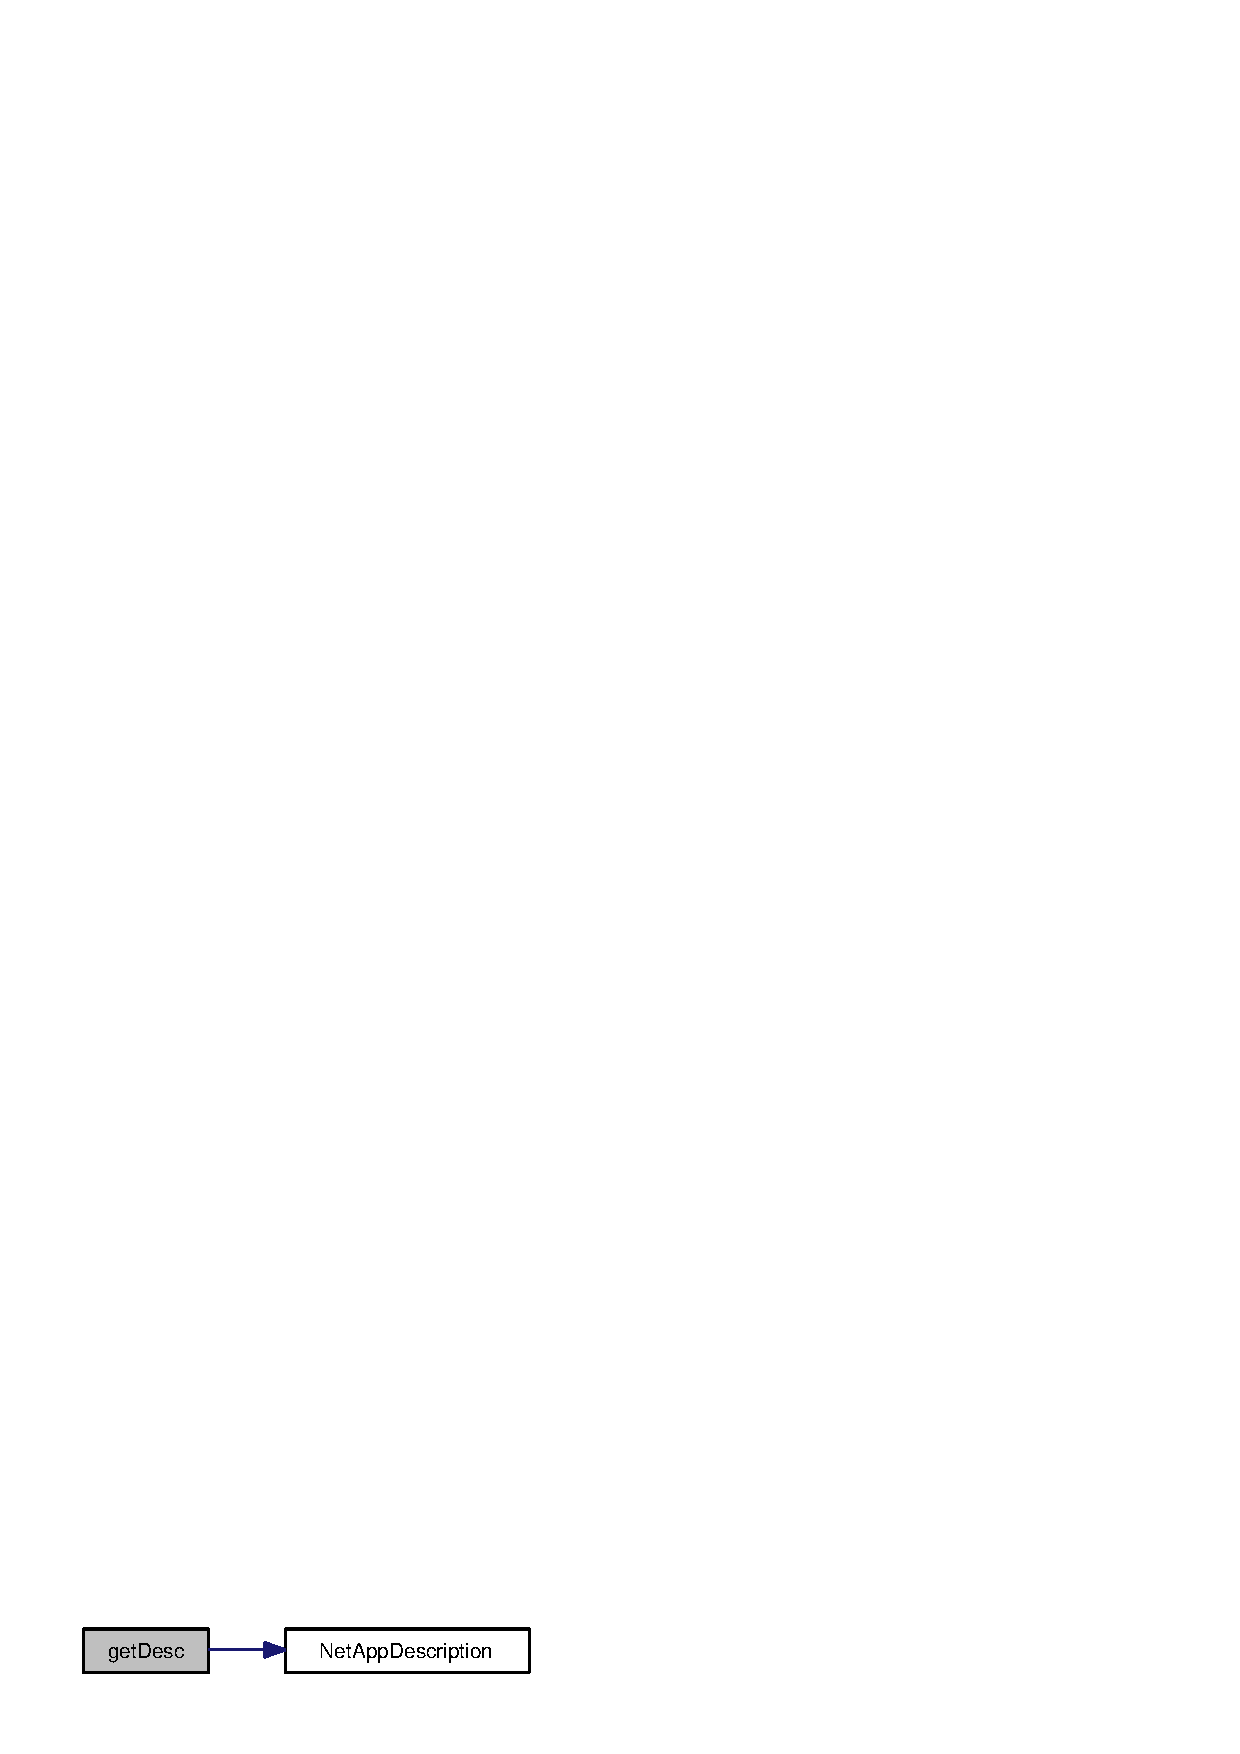
\includegraphics[width=258pt]{classorg_1_1smallfoot_1_1wwn_1_1NetAppDescription_a7e34be4d9bd11a9971c007c6231b8c01_cgraph}
\end{center}
\end{figure}


\index{org\-::smallfoot\-::wwn\-::\-Net\-App\-Description@{org\-::smallfoot\-::wwn\-::\-Net\-App\-Description}!to\-String@{to\-String}}
\index{to\-String@{to\-String}!org::smallfoot::wwn::NetAppDescription@{org\-::smallfoot\-::wwn\-::\-Net\-App\-Description}}
\subsubsection[{to\-String}]{\setlength{\rightskip}{0pt plus 5cm}String to\-String (
\begin{DoxyParamCaption}
{}
\end{DoxyParamCaption}
)\hspace{0.3cm}{\ttfamily [inline]}}\label{classorg_1_1smallfoot_1_1wwn_1_1NetAppDescription_ad146fa8579a5f8a876c4688cc5a68520}


return a description or alias for this W\-W\-N; if brief is set to true during the call to \doxyref{get\-Desc()}{p.}{classorg_1_1smallfoot_1_1wwn_1_1NetAppDescription_a7e34be4d9bd11a9971c007c6231b8c01}, then a shorter description or alias will be returned 

\begin{DoxySeeAlso}{See Also}
\doxyref{get\-Desc(boolean,boolean,\-String)}{p.}{classorg_1_1smallfoot_1_1wwn_1_1NetAppDescription_a7e34be4d9bd11a9971c007c6231b8c01}
\end{DoxySeeAlso}
\begin{DoxyReturn}{Returns}
generated alias or nickname for the W\-W\-N 
\end{DoxyReturn}


Definition at line 50 of file Net\-App\-Description.\-java.



References W\-W\-N\-Desc.\-brief.



The documentation for this class was generated from the following file\-:\begin{DoxyCompactItemize}
\item 
java/{\bf Net\-App\-Description.\-java}\end{DoxyCompactItemize}

\section{Oracle\+Pillar\+Description Class Reference}
\label{classorg_1_1smallfoot_1_1wwn_1_1OraclePillarDescription}\index{Oracle\+Pillar\+Description@{Oracle\+Pillar\+Description}}


Descriptor for (Oracle) Pillar Data Systems\textquotesingle{} Service Lifecycle Management devices.  




Inheritance diagram for Oracle\+Pillar\+Description\+:\nopagebreak
\begin{figure}[H]
\begin{center}
\leavevmode
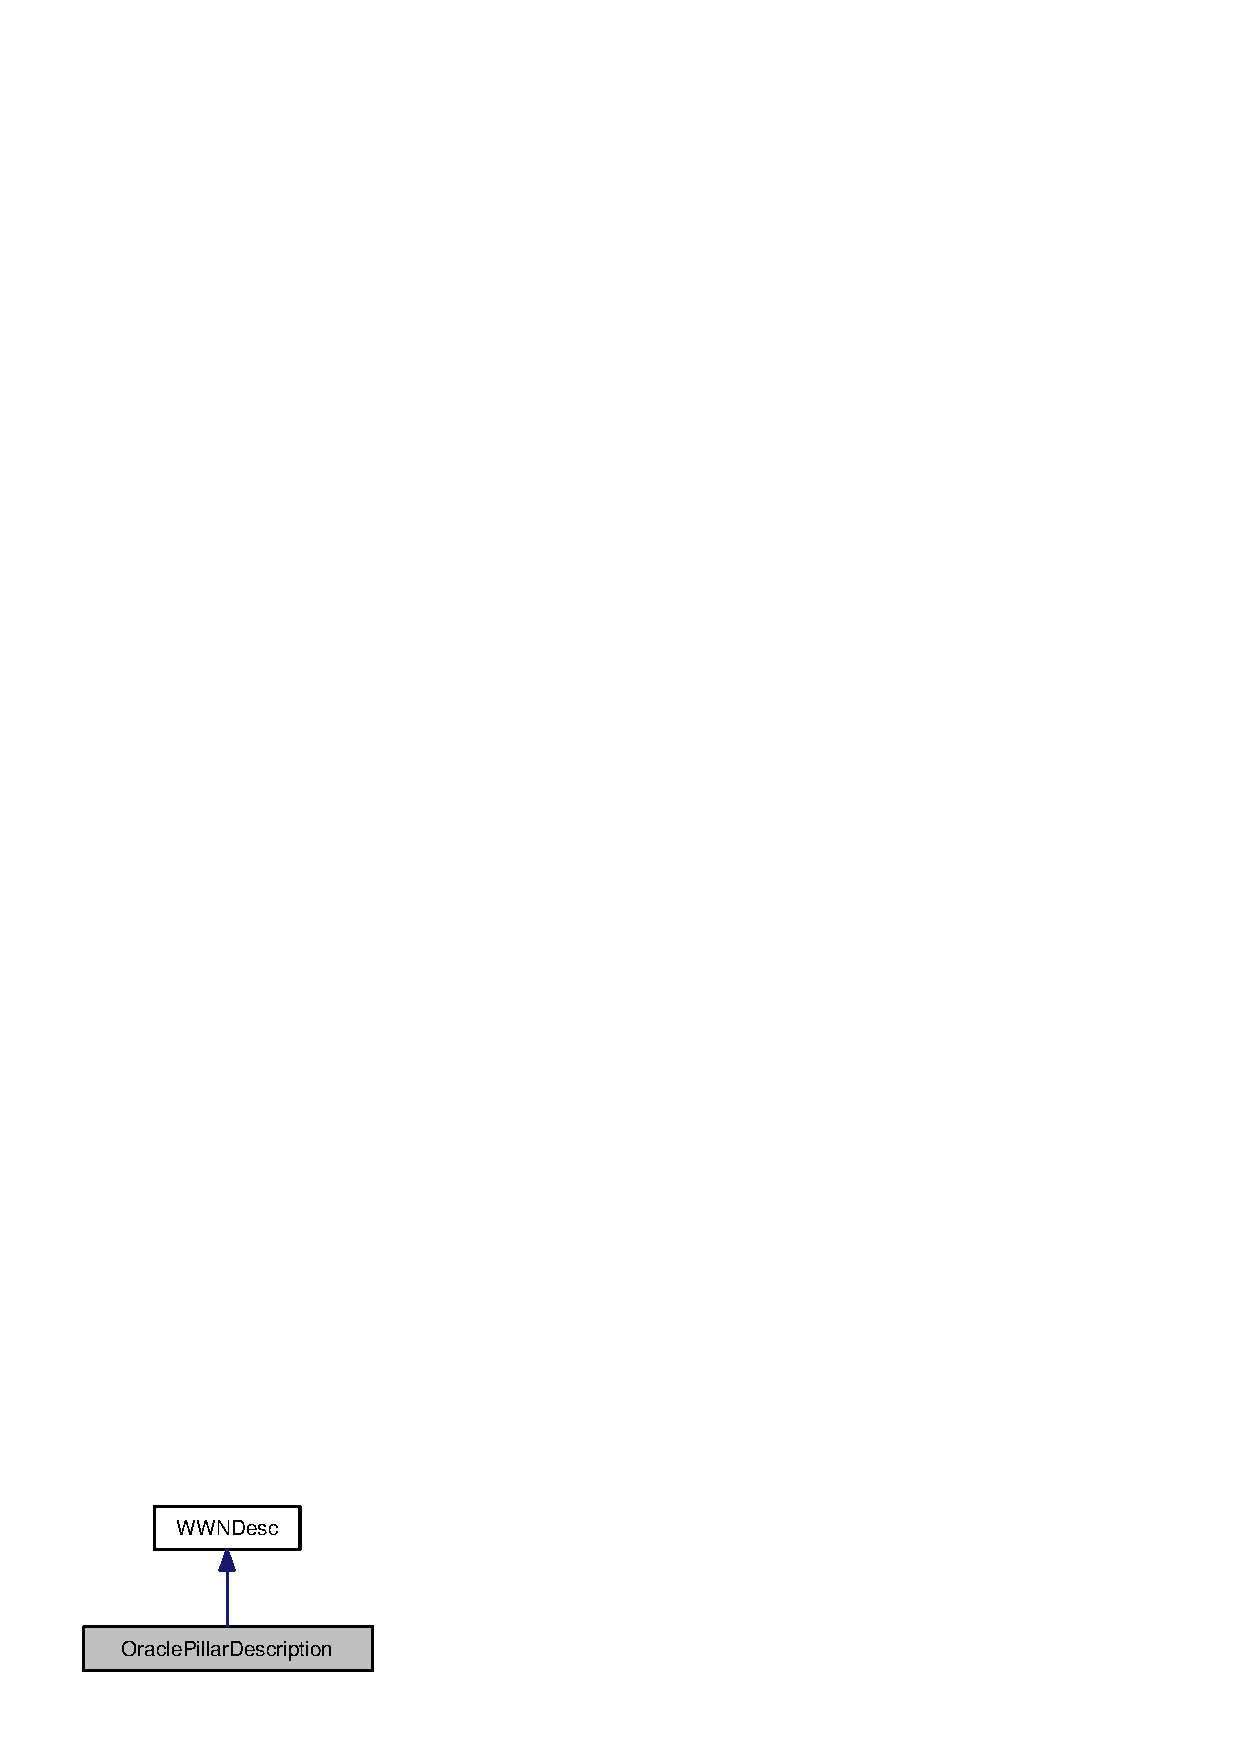
\includegraphics[width=190pt]{classorg_1_1smallfoot_1_1wwn_1_1OraclePillarDescription__inherit__graph}
\end{center}
\end{figure}


Collaboration diagram for Oracle\+Pillar\+Description\+:\nopagebreak
\begin{figure}[H]
\begin{center}
\leavevmode
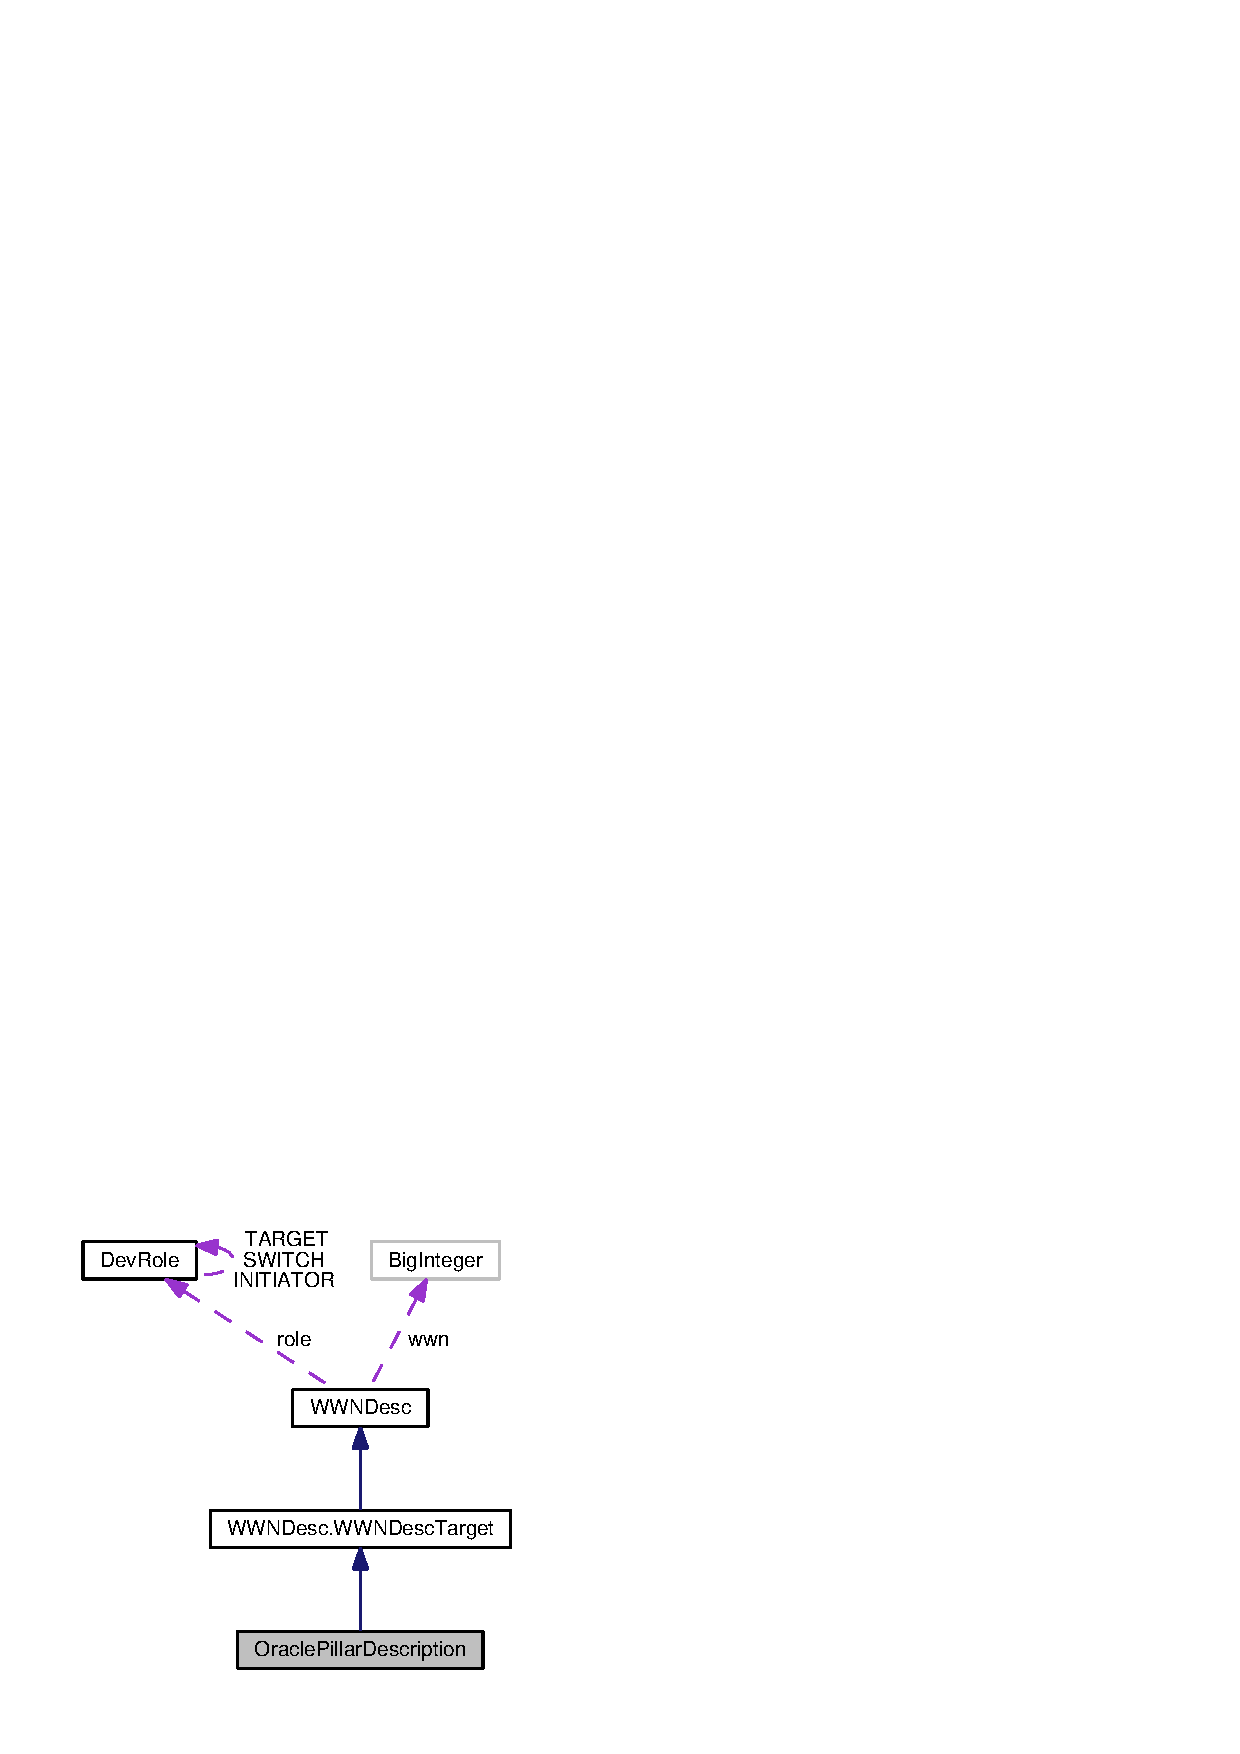
\includegraphics[width=253pt]{classorg_1_1smallfoot_1_1wwn_1_1OraclePillarDescription__coll__graph}
\end{center}
\end{figure}
\subsection*{Public Member Functions}
\begin{DoxyCompactItemize}
\item 
{\bf Oracle\+Pillar\+Description} (String {\bf wwn})
\begin{DoxyCompactList}\small\item\em create an instance with \doxyref{brief}{p.}{classorg_1_1smallfoot_1_1wwn_1_1WWNDesc_adbebed411e8c47d43338efa3edaa13f8} set to false. \end{DoxyCompactList}\item 
String {\bf to\+String} ()
\begin{DoxyCompactList}\small\item\em return a description or alias for this W\+W\+N \end{DoxyCompactList}\end{DoxyCompactItemize}
\subsection*{Static Public Member Functions}
\begin{DoxyCompactItemize}
\item 
static {\bf W\+W\+N\+Desc} {\bf get\+Desc} (boolean strong, boolean {\bf brief}, String {\bf wwn})
\begin{DoxyCompactList}\small\item\em If this class matches or describes the given W\+W\+N, returns a new instance of this class loaded with the given W\+W\+N. \end{DoxyCompactList}\item 
static {\bf W\+W\+N\+Desc} {\bf get\+Desc} (boolean strong, boolean {\bf brief}, String {\bf wwn}, int {\bf role})
\begin{DoxyCompactList}\small\item\em If this class matches or describes the given W\+W\+N, returns a new instance of this class loaded with the given W\+W\+N. \end{DoxyCompactList}\end{DoxyCompactItemize}
\subsection*{Additional Inherited Members}


\subsection{Detailed Description}
Descriptor for (Oracle) Pillar Data Systems\textquotesingle{} Service Lifecycle Management devices. 

Definition at line 13 of file Oracle\+Pillar\+Description.\+java.



\subsection{Constructor \& Destructor Documentation}
\index{org\+::smallfoot\+::wwn\+::\+Oracle\+Pillar\+Description@{org\+::smallfoot\+::wwn\+::\+Oracle\+Pillar\+Description}!Oracle\+Pillar\+Description@{Oracle\+Pillar\+Description}}
\index{Oracle\+Pillar\+Description@{Oracle\+Pillar\+Description}!org\+::smallfoot\+::wwn\+::\+Oracle\+Pillar\+Description@{org\+::smallfoot\+::wwn\+::\+Oracle\+Pillar\+Description}}
\subsubsection[{Oracle\+Pillar\+Description}]{\setlength{\rightskip}{0pt plus 5cm}{\bf Oracle\+Pillar\+Description} (
\begin{DoxyParamCaption}
\item[{String}]{wwn}
\end{DoxyParamCaption}
)\hspace{0.3cm}{\ttfamily [inline]}}\label{classorg_1_1smallfoot_1_1wwn_1_1OraclePillarDescription_a18e4afcfc6772a559d0e3ad342315eaa}


create an instance with \doxyref{brief}{p.}{classorg_1_1smallfoot_1_1wwn_1_1WWNDesc_adbebed411e8c47d43338efa3edaa13f8} set to false. 

This is a convenience function to support the older constructor model


\begin{DoxyExceptions}{Exceptions}
{\em java.\+lang.\+Null\+Pointer\+Exception} & if the given wwn is null\\
\hline
\end{DoxyExceptions}

\begin{DoxyParams}{Parameters}
{\em wwn} & the W\+W\+N to evaluate and describe \\
\hline
\end{DoxyParams}


Definition at line 16 of file Oracle\+Pillar\+Description.\+java.



Referenced by Oracle\+Pillar\+Description.\+get\+Desc().



\subsection{Member Function Documentation}
\index{org\+::smallfoot\+::wwn\+::\+Oracle\+Pillar\+Description@{org\+::smallfoot\+::wwn\+::\+Oracle\+Pillar\+Description}!get\+Desc@{get\+Desc}}
\index{get\+Desc@{get\+Desc}!org\+::smallfoot\+::wwn\+::\+Oracle\+Pillar\+Description@{org\+::smallfoot\+::wwn\+::\+Oracle\+Pillar\+Description}}
\subsubsection[{get\+Desc}]{\setlength{\rightskip}{0pt plus 5cm}static {\bf W\+W\+N\+Desc} get\+Desc (
\begin{DoxyParamCaption}
\item[{boolean}]{strong, }
\item[{boolean}]{brief, }
\item[{String}]{wwn}
\end{DoxyParamCaption}
)\hspace{0.3cm}{\ttfamily [inline]}, {\ttfamily [static]}}\label{classorg_1_1smallfoot_1_1wwn_1_1OraclePillarDescription_a7e34be4d9bd11a9971c007c6231b8c01}


If this class matches or describes the given W\+W\+N, returns a new instance of this class loaded with the given W\+W\+N. 

\begin{DoxyReturn}{Returns}
new instance of this class, or null if the given wwn does not match this class 
\end{DoxyReturn}

\begin{DoxyParams}{Parameters}
{\em strong} & is ignored\+: this class is a strong representation, not a weak one based on empirical matching, hence can always be used with confidence \\
\hline
{\em brief} & is ignored\+: this class has only one representation of the W\+W\+N description or alias \\
\hline
{\em wwn} & the W\+W\+N (W\+W\+P\+N or W\+W\+N\+N, but typically W\+W\+P\+N) to match \\
\hline
\end{DoxyParams}


Definition at line 29 of file Oracle\+Pillar\+Description.\+java.



References Dev\+Role.\+max.



Referenced by W\+W\+N\+Description.\+get\+W\+W\+N\+Descriptor().

\index{org\+::smallfoot\+::wwn\+::\+Oracle\+Pillar\+Description@{org\+::smallfoot\+::wwn\+::\+Oracle\+Pillar\+Description}!get\+Desc@{get\+Desc}}
\index{get\+Desc@{get\+Desc}!org\+::smallfoot\+::wwn\+::\+Oracle\+Pillar\+Description@{org\+::smallfoot\+::wwn\+::\+Oracle\+Pillar\+Description}}
\subsubsection[{get\+Desc}]{\setlength{\rightskip}{0pt plus 5cm}static {\bf W\+W\+N\+Desc} get\+Desc (
\begin{DoxyParamCaption}
\item[{boolean}]{strong, }
\item[{boolean}]{brief, }
\item[{String}]{wwn, }
\item[{int}]{role}
\end{DoxyParamCaption}
)\hspace{0.3cm}{\ttfamily [inline]}, {\ttfamily [static]}}\label{classorg_1_1smallfoot_1_1wwn_1_1OraclePillarDescription_a37ac294533314b3b7b3a5f3404ee43d6}


If this class matches or describes the given W\+W\+N, returns a new instance of this class loaded with the given W\+W\+N. 

\begin{DoxyReturn}{Returns}
new instance of this class, or null if the given wwn does not match this class 
\end{DoxyReturn}

\begin{DoxyParams}{Parameters}
{\em strong} & is ignored\+: this class is a strong representation, not a weak one based on empirical matching, hence can always be used with confidence \\
\hline
{\em brief} & is ignored\+: this class has only one representation of the W\+W\+N description or alias \\
\hline
{\em wwn} & the W\+W\+N (W\+W\+P\+N or W\+W\+N\+N, but typically W\+W\+P\+N) to match \\
\hline
{\em role} & Role (Initiator/\+Switch/\+Target) to check for \\
\hline
\end{DoxyParams}


Definition at line 37 of file Oracle\+Pillar\+Description.\+java.



References W\+W\+N\+Desc.\+W\+W\+N\+Desc\+Target.\+is\+A(), and Oracle\+Pillar\+Description.\+Oracle\+Pillar\+Description().



Here is the call graph for this function\+:\nopagebreak
\begin{figure}[H]
\begin{center}
\leavevmode
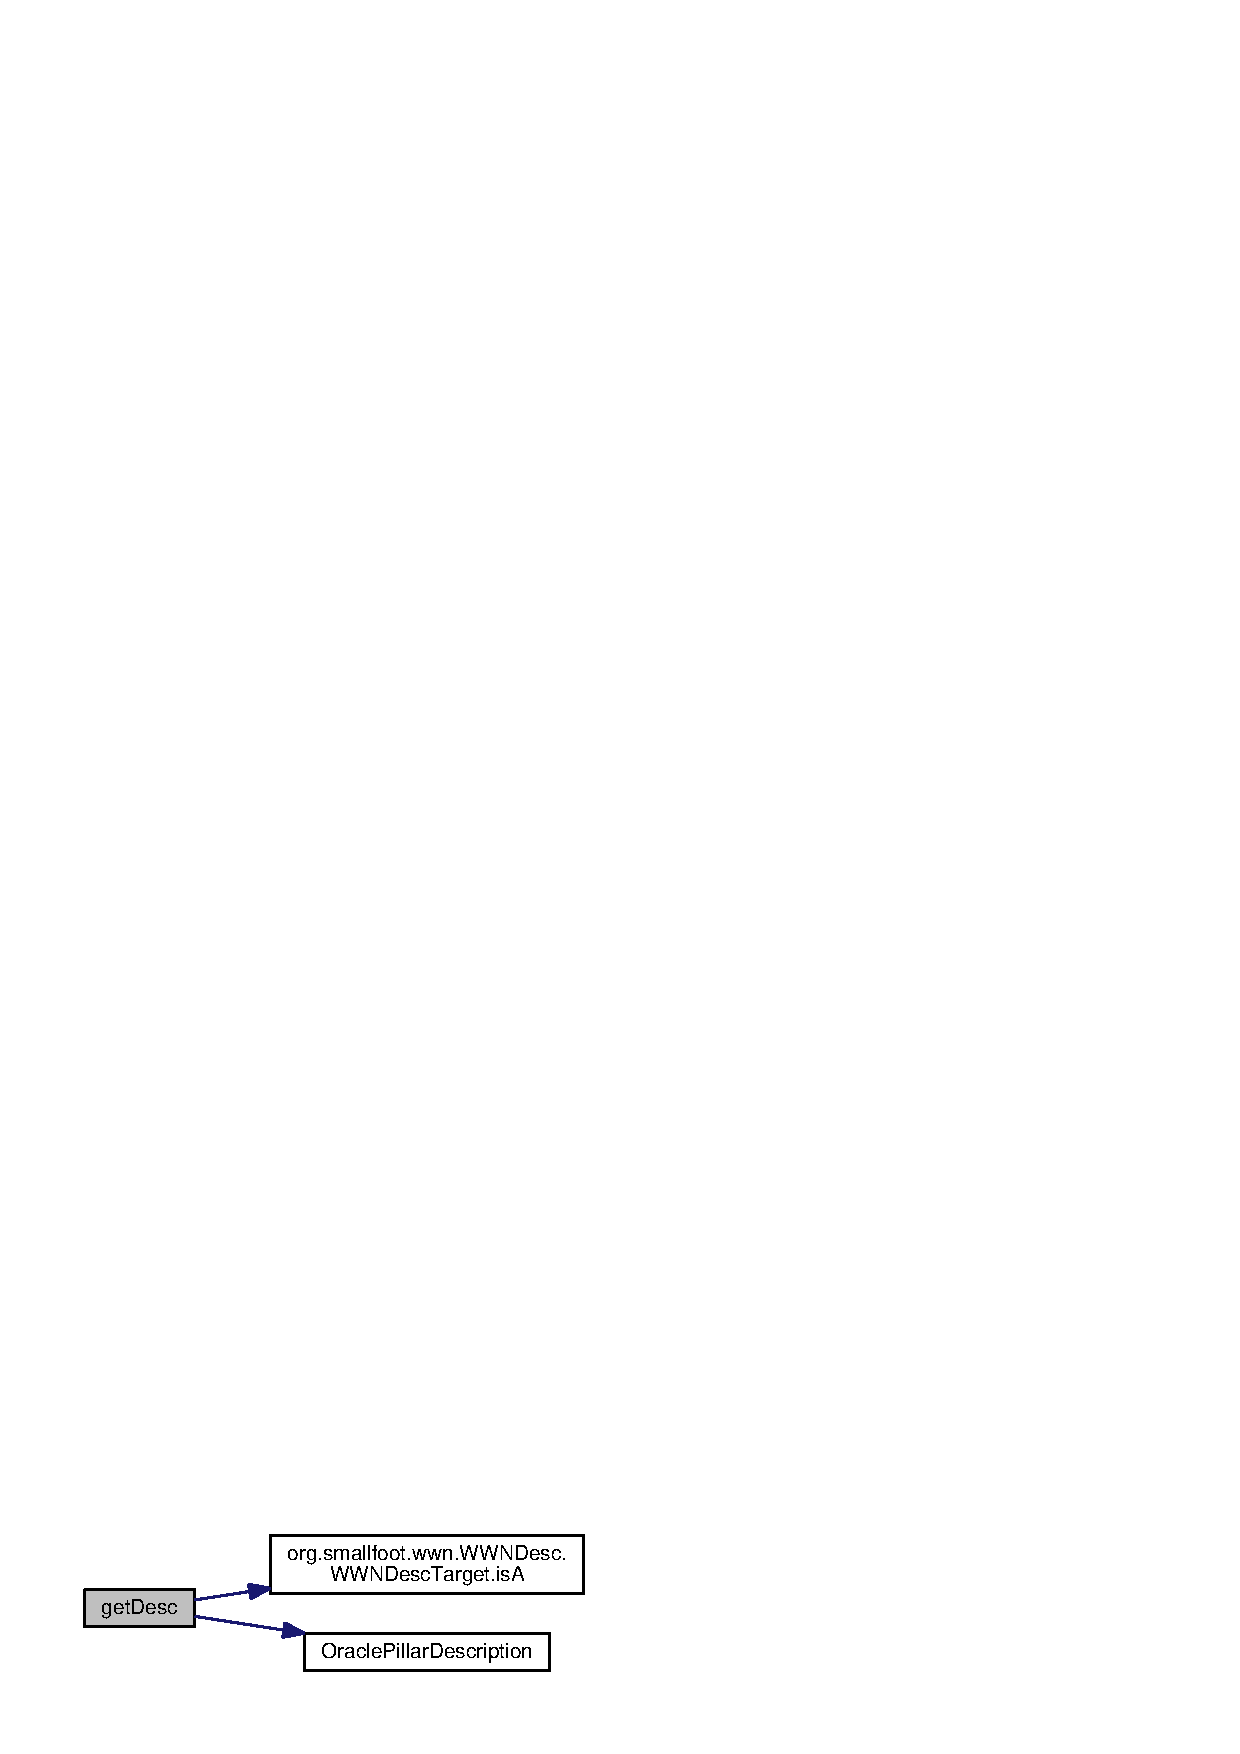
\includegraphics[width=284pt]{classorg_1_1smallfoot_1_1wwn_1_1OraclePillarDescription_a37ac294533314b3b7b3a5f3404ee43d6_cgraph}
\end{center}
\end{figure}


\index{org\+::smallfoot\+::wwn\+::\+Oracle\+Pillar\+Description@{org\+::smallfoot\+::wwn\+::\+Oracle\+Pillar\+Description}!to\+String@{to\+String}}
\index{to\+String@{to\+String}!org\+::smallfoot\+::wwn\+::\+Oracle\+Pillar\+Description@{org\+::smallfoot\+::wwn\+::\+Oracle\+Pillar\+Description}}
\subsubsection[{to\+String}]{\setlength{\rightskip}{0pt plus 5cm}String to\+String (
\begin{DoxyParamCaption}
{}
\end{DoxyParamCaption}
)\hspace{0.3cm}{\ttfamily [inline]}}\label{classorg_1_1smallfoot_1_1wwn_1_1OraclePillarDescription_ad146fa8579a5f8a876c4688cc5a68520}


return a description or alias for this W\+W\+N 

\begin{DoxyReturn}{Returns}
generated alias or nickname for the W\+W\+N 
\end{DoxyReturn}


Definition at line 52 of file Oracle\+Pillar\+Description.\+java.



References W\+W\+N\+Desc.\+wwn.



The documentation for this class was generated from the following file\+:\begin{DoxyCompactItemize}
\item 
java/{\bf Oracle\+Pillar\+Description.\+java}\end{DoxyCompactItemize}

\section{Pure\-Storage\-Description Class Reference}
\label{classorg_1_1smallfoot_1_1wwn_1_1PureStorageDescription}\index{Pure\-Storage\-Description@{Pure\-Storage\-Description}}


Inheritance diagram for Pure\-Storage\-Description\-:\nopagebreak
\begin{figure}[H]
\begin{center}
\leavevmode
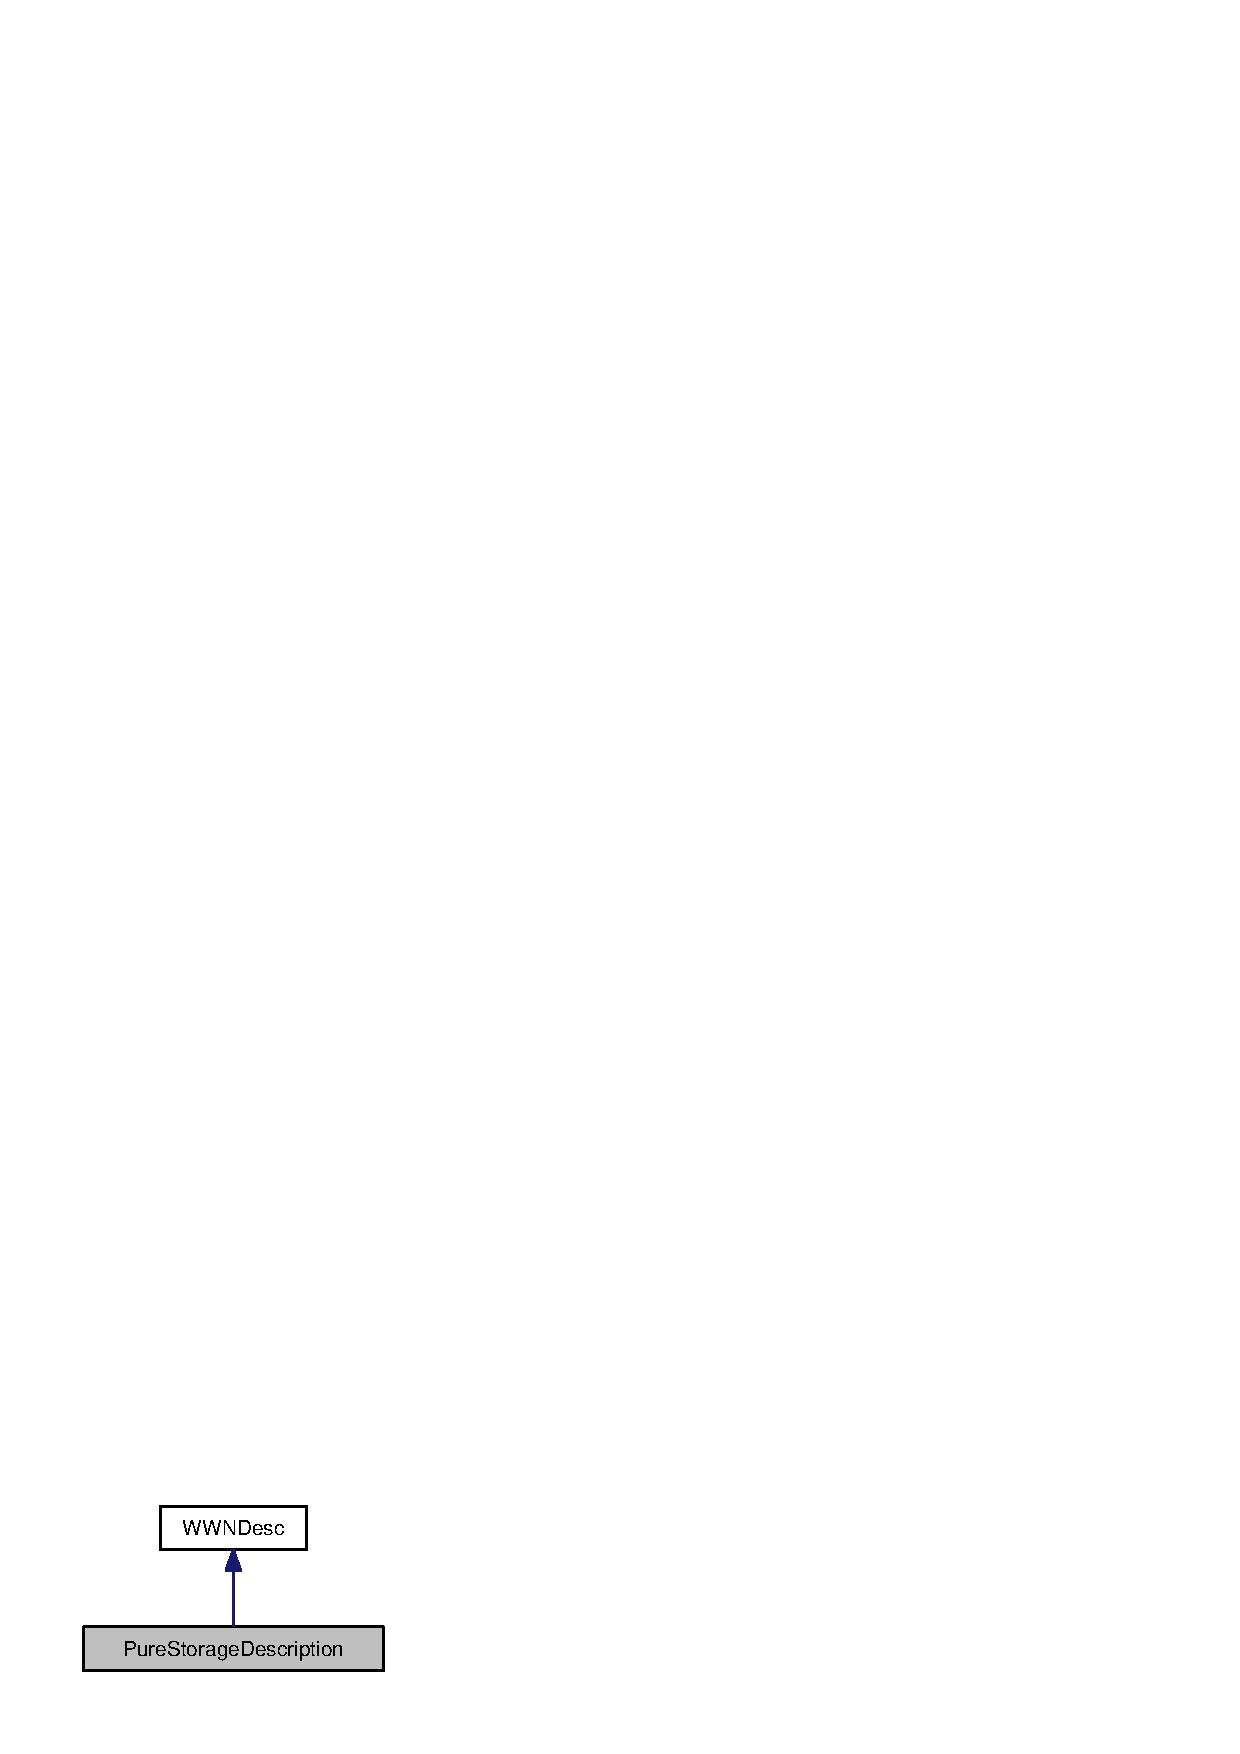
\includegraphics[width=188pt]{classorg_1_1smallfoot_1_1wwn_1_1PureStorageDescription__inherit__graph}
\end{center}
\end{figure}


Collaboration diagram for Pure\-Storage\-Description\-:\nopagebreak
\begin{figure}[H]
\begin{center}
\leavevmode
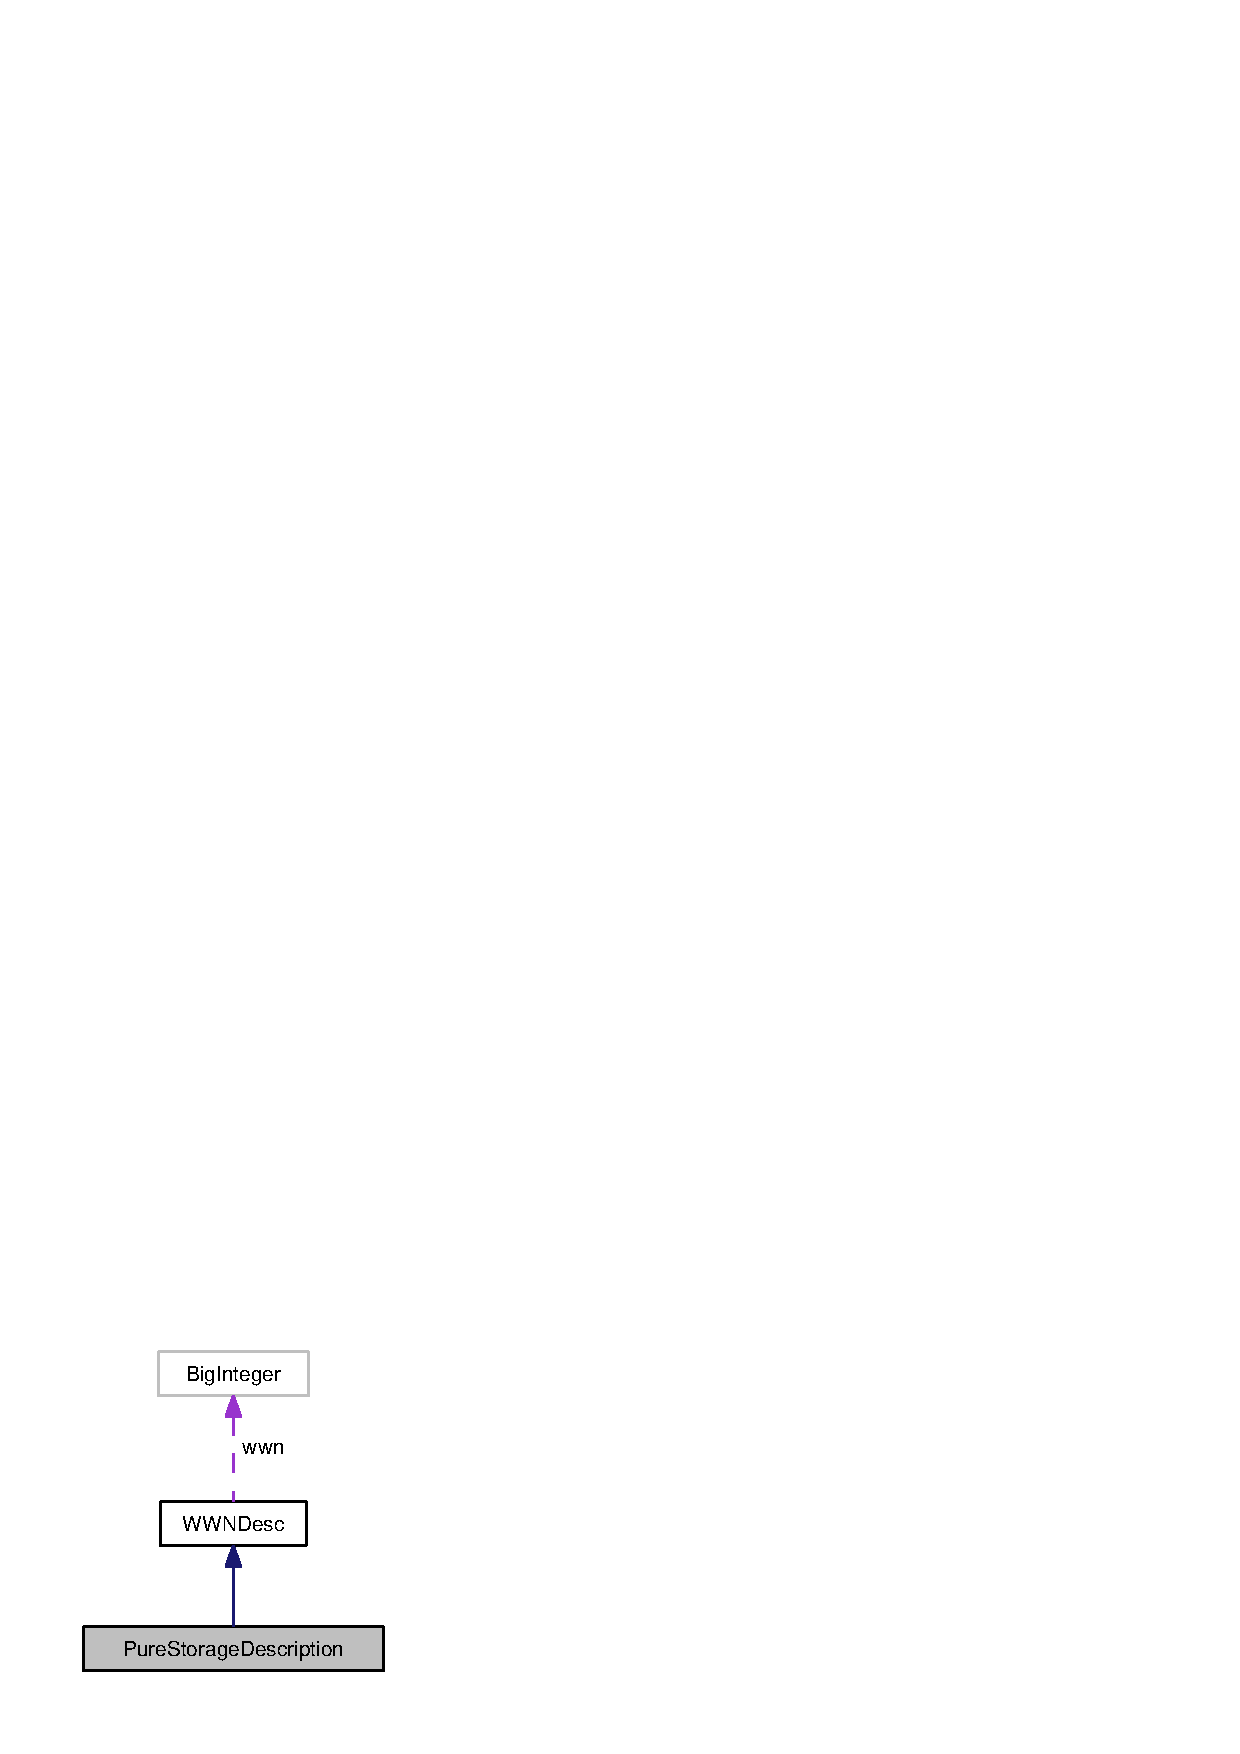
\includegraphics[width=188pt]{classorg_1_1smallfoot_1_1wwn_1_1PureStorageDescription__coll__graph}
\end{center}
\end{figure}
\subsection*{Public Member Functions}
\begin{DoxyCompactItemize}
\item 
{\bf Pure\-Storage\-Description} (String wwn)
\begin{DoxyCompactList}\small\item\em create an instance with this.\-brief set to false. \end{DoxyCompactList}\item 
{\bf Pure\-Storage\-Description} (boolean brief, String wwn)
\begin{DoxyCompactList}\small\item\em create an instance with the given W\-W\-N. \end{DoxyCompactList}\item 
String {\bf to\-String} ()
\begin{DoxyCompactList}\small\item\em return a description or alias for this W\-W\-N; if brief is set to true during the call to \doxyref{get\-Desc()}{p.}{classorg_1_1smallfoot_1_1wwn_1_1PureStorageDescription_a7e34be4d9bd11a9971c007c6231b8c01}, then a shorter description or alias will be returned \end{DoxyCompactList}\end{DoxyCompactItemize}
\subsection*{Static Public Member Functions}
\begin{DoxyCompactItemize}
\item 
static {\bf W\-W\-N\-Desc} {\bf get\-Desc} (boolean strong, boolean brief, String wwn)
\begin{DoxyCompactList}\small\item\em If this class matches or describes the given W\-W\-N, returns a new instance of this class loaded with the given W\-W\-N. \end{DoxyCompactList}\end{DoxyCompactItemize}


\subsection{Detailed Description}


Definition at line 6 of file Pure\-Storage\-Description.\-java.



\subsection{Constructor \& Destructor Documentation}
\index{org\-::smallfoot\-::wwn\-::\-Pure\-Storage\-Description@{org\-::smallfoot\-::wwn\-::\-Pure\-Storage\-Description}!Pure\-Storage\-Description@{Pure\-Storage\-Description}}
\index{Pure\-Storage\-Description@{Pure\-Storage\-Description}!org::smallfoot::wwn::PureStorageDescription@{org\-::smallfoot\-::wwn\-::\-Pure\-Storage\-Description}}
\subsubsection[{Pure\-Storage\-Description}]{\setlength{\rightskip}{0pt plus 5cm}{\bf Pure\-Storage\-Description} (
\begin{DoxyParamCaption}
\item[{String}]{wwn}
\end{DoxyParamCaption}
)\hspace{0.3cm}{\ttfamily [inline]}}\label{classorg_1_1smallfoot_1_1wwn_1_1PureStorageDescription_a72a5ef8310289be76088199c473b607a}


create an instance with this.\-brief set to false. 

This is a convenience function to support the older constructor model


\begin{DoxyParams}{Parameters}
{\em wwn} & the W\-W\-N to evaluate and describe \\
\hline
\end{DoxyParams}


Definition at line 9 of file Pure\-Storage\-Description.\-java.



Referenced by Pure\-Storage\-Description.\-get\-Desc().

\index{org\-::smallfoot\-::wwn\-::\-Pure\-Storage\-Description@{org\-::smallfoot\-::wwn\-::\-Pure\-Storage\-Description}!Pure\-Storage\-Description@{Pure\-Storage\-Description}}
\index{Pure\-Storage\-Description@{Pure\-Storage\-Description}!org::smallfoot::wwn::PureStorageDescription@{org\-::smallfoot\-::wwn\-::\-Pure\-Storage\-Description}}
\subsubsection[{Pure\-Storage\-Description}]{\setlength{\rightskip}{0pt plus 5cm}{\bf Pure\-Storage\-Description} (
\begin{DoxyParamCaption}
\item[{boolean}]{brief, }
\item[{String}]{wwn}
\end{DoxyParamCaption}
)\hspace{0.3cm}{\ttfamily [inline]}}\label{classorg_1_1smallfoot_1_1wwn_1_1PureStorageDescription_a2ea6fcaaa1974c68217380fa6667f564}


create an instance with the given W\-W\-N. 

Values given to the constructor are simply copied to internal variables for later use


\begin{DoxyParams}{Parameters}
{\em brief} & whether an abbreviated description is requested \\
\hline
{\em wwn} & the W\-W\-N to evaluate and describe \\
\hline
\end{DoxyParams}


Definition at line 33 of file Pure\-Storage\-Description.\-java.



\subsection{Member Function Documentation}
\index{org\-::smallfoot\-::wwn\-::\-Pure\-Storage\-Description@{org\-::smallfoot\-::wwn\-::\-Pure\-Storage\-Description}!get\-Desc@{get\-Desc}}
\index{get\-Desc@{get\-Desc}!org::smallfoot::wwn::PureStorageDescription@{org\-::smallfoot\-::wwn\-::\-Pure\-Storage\-Description}}
\subsubsection[{get\-Desc}]{\setlength{\rightskip}{0pt plus 5cm}static {\bf W\-W\-N\-Desc} get\-Desc (
\begin{DoxyParamCaption}
\item[{boolean}]{strong, }
\item[{boolean}]{brief, }
\item[{String}]{wwn}
\end{DoxyParamCaption}
)\hspace{0.3cm}{\ttfamily [inline]}, {\ttfamily [static]}}\label{classorg_1_1smallfoot_1_1wwn_1_1PureStorageDescription_a7e34be4d9bd11a9971c007c6231b8c01}


If this class matches or describes the given W\-W\-N, returns a new instance of this class loaded with the given W\-W\-N. 

\begin{DoxyReturn}{Returns}
new instance of this class, or null if the given wwn does not match this class 
\end{DoxyReturn}

\begin{DoxyParams}{Parameters}
{\em strong} & used to restrict matching to strong-\/matches only. This is a weak-\/confidence description, so will return null for strong-\/only matching \\
\hline
{\em brief} & is used to ask for a shorter description\-: a more concise nickname or alias \\
\hline
{\em wwn} & the W\-W\-N (W\-W\-P\-N or W\-W\-N\-N, but typically W\-W\-P\-N) to match \\
\hline
\end{DoxyParams}


Definition at line 22 of file Pure\-Storage\-Description.\-java.



References Pure\-Storage\-Description.\-Pure\-Storage\-Description().



Referenced by W\-W\-N\-Description.\-get\-W\-W\-N\-Descriptor().



Here is the call graph for this function\-:\nopagebreak
\begin{figure}[H]
\begin{center}
\leavevmode
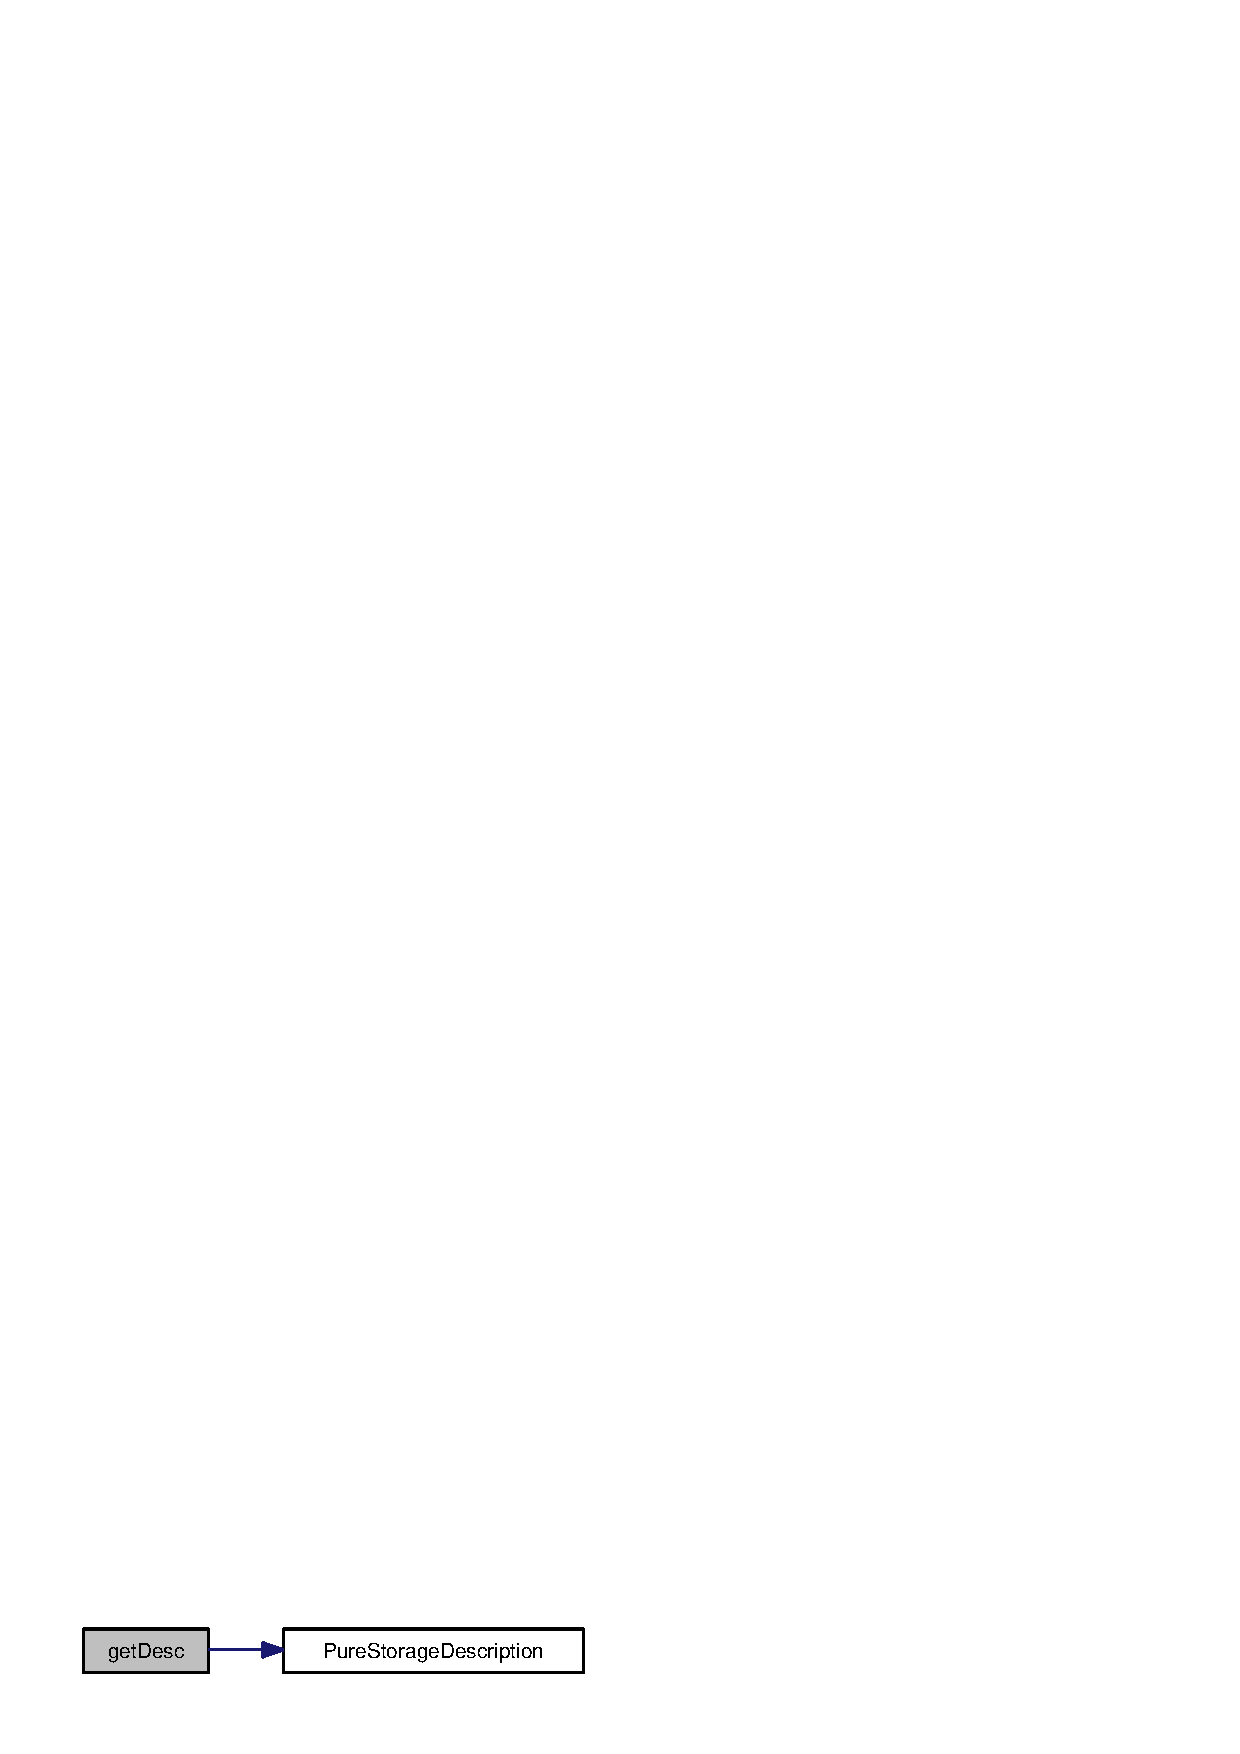
\includegraphics[width=284pt]{classorg_1_1smallfoot_1_1wwn_1_1PureStorageDescription_a7e34be4d9bd11a9971c007c6231b8c01_cgraph}
\end{center}
\end{figure}


\index{org\-::smallfoot\-::wwn\-::\-Pure\-Storage\-Description@{org\-::smallfoot\-::wwn\-::\-Pure\-Storage\-Description}!to\-String@{to\-String}}
\index{to\-String@{to\-String}!org::smallfoot::wwn::PureStorageDescription@{org\-::smallfoot\-::wwn\-::\-Pure\-Storage\-Description}}
\subsubsection[{to\-String}]{\setlength{\rightskip}{0pt plus 5cm}String to\-String (
\begin{DoxyParamCaption}
{}
\end{DoxyParamCaption}
)\hspace{0.3cm}{\ttfamily [inline]}}\label{classorg_1_1smallfoot_1_1wwn_1_1PureStorageDescription_ad146fa8579a5f8a876c4688cc5a68520}


return a description or alias for this W\-W\-N; if brief is set to true during the call to \doxyref{get\-Desc()}{p.}{classorg_1_1smallfoot_1_1wwn_1_1PureStorageDescription_a7e34be4d9bd11a9971c007c6231b8c01}, then a shorter description or alias will be returned 

\begin{DoxySeeAlso}{See Also}
\doxyref{get\-Desc(boolean,boolean,\-String)}{p.}{classorg_1_1smallfoot_1_1wwn_1_1PureStorageDescription_a7e34be4d9bd11a9971c007c6231b8c01}
\end{DoxySeeAlso}
\begin{DoxyReturn}{Returns}
generated alias or nickname for the W\-W\-N 
\end{DoxyReturn}


Definition at line 44 of file Pure\-Storage\-Description.\-java.



The documentation for this class was generated from the following file\-:\begin{DoxyCompactItemize}
\item 
java/Pure\-Storage\-Description.\-java\end{DoxyCompactItemize}

\section{version Class Reference}
\label{classorg_1_1smallfoot_1_1wwn_1_1version}\index{version@{version}}


version is used to allow a package that uses this package to be able to \char`\"{}ask\char`\"{} the jar file what version it is  


\subsection*{Static Public Member Functions}
\begin{DoxyCompactItemize}
\item 
static void {\bf main} (String arg[$\,$])
\begin{DoxyCompactList}\small\item\em returns the version of the class; used to cause the build-\/time-\/detected version and buildid to be available by consumers of the generated wwndesc.\+jar file \end{DoxyCompactList}\end{DoxyCompactItemize}


\subsection{Detailed Description}
version is used to allow a package that uses this package to be able to \char`\"{}ask\char`\"{} the jar file what version it is 

Definition at line 8 of file version.\+java.



\subsection{Member Function Documentation}
\index{org\+::smallfoot\+::wwn\+::version@{org\+::smallfoot\+::wwn\+::version}!main@{main}}
\index{main@{main}!org\+::smallfoot\+::wwn\+::version@{org\+::smallfoot\+::wwn\+::version}}
\subsubsection[{main}]{\setlength{\rightskip}{0pt plus 5cm}static void main (
\begin{DoxyParamCaption}
\item[{String}]{arg[$\,$]}
\end{DoxyParamCaption}
)\hspace{0.3cm}{\ttfamily [inline]}, {\ttfamily [static]}}\label{classorg_1_1smallfoot_1_1wwn_1_1version_ae4faf7ff4190d227357ef851490d7757}


returns the version of the class; used to cause the build-\/time-\/detected version and buildid to be available by consumers of the generated wwndesc.\+jar file 

for example\+: java -\/cp wwndesc.\+jar \doxyref{org.\+smallfoot.\+wwn.\+version}{p.}{classorg_1_1smallfoot_1_1wwn_1_1version} 1.\+0.\+62


\begin{DoxyParams}{Parameters}
{\em arg} & ignored \\
\hline
\end{DoxyParams}


Definition at line 19 of file version.\+java.



The documentation for this class was generated from the following file\+:\begin{DoxyCompactItemize}
\item 
java/{\bf version.\+java}\end{DoxyCompactItemize}

\section{W\-W\-N\-Desc Class Reference}
\label{classorg_1_1smallfoot_1_1wwn_1_1WWNDesc}\index{W\-W\-N\-Desc@{W\-W\-N\-Desc}}


\doxyref{W\-W\-N\-Desc}{p.}{classorg_1_1smallfoot_1_1wwn_1_1WWNDesc} is the basic generic class from which each vendor-\/specific pattern is built upon; similar to an abstract parent but populated methods.  




Inheritance diagram for W\-W\-N\-Desc\-:\nopagebreak
\begin{figure}[H]
\begin{center}
\leavevmode
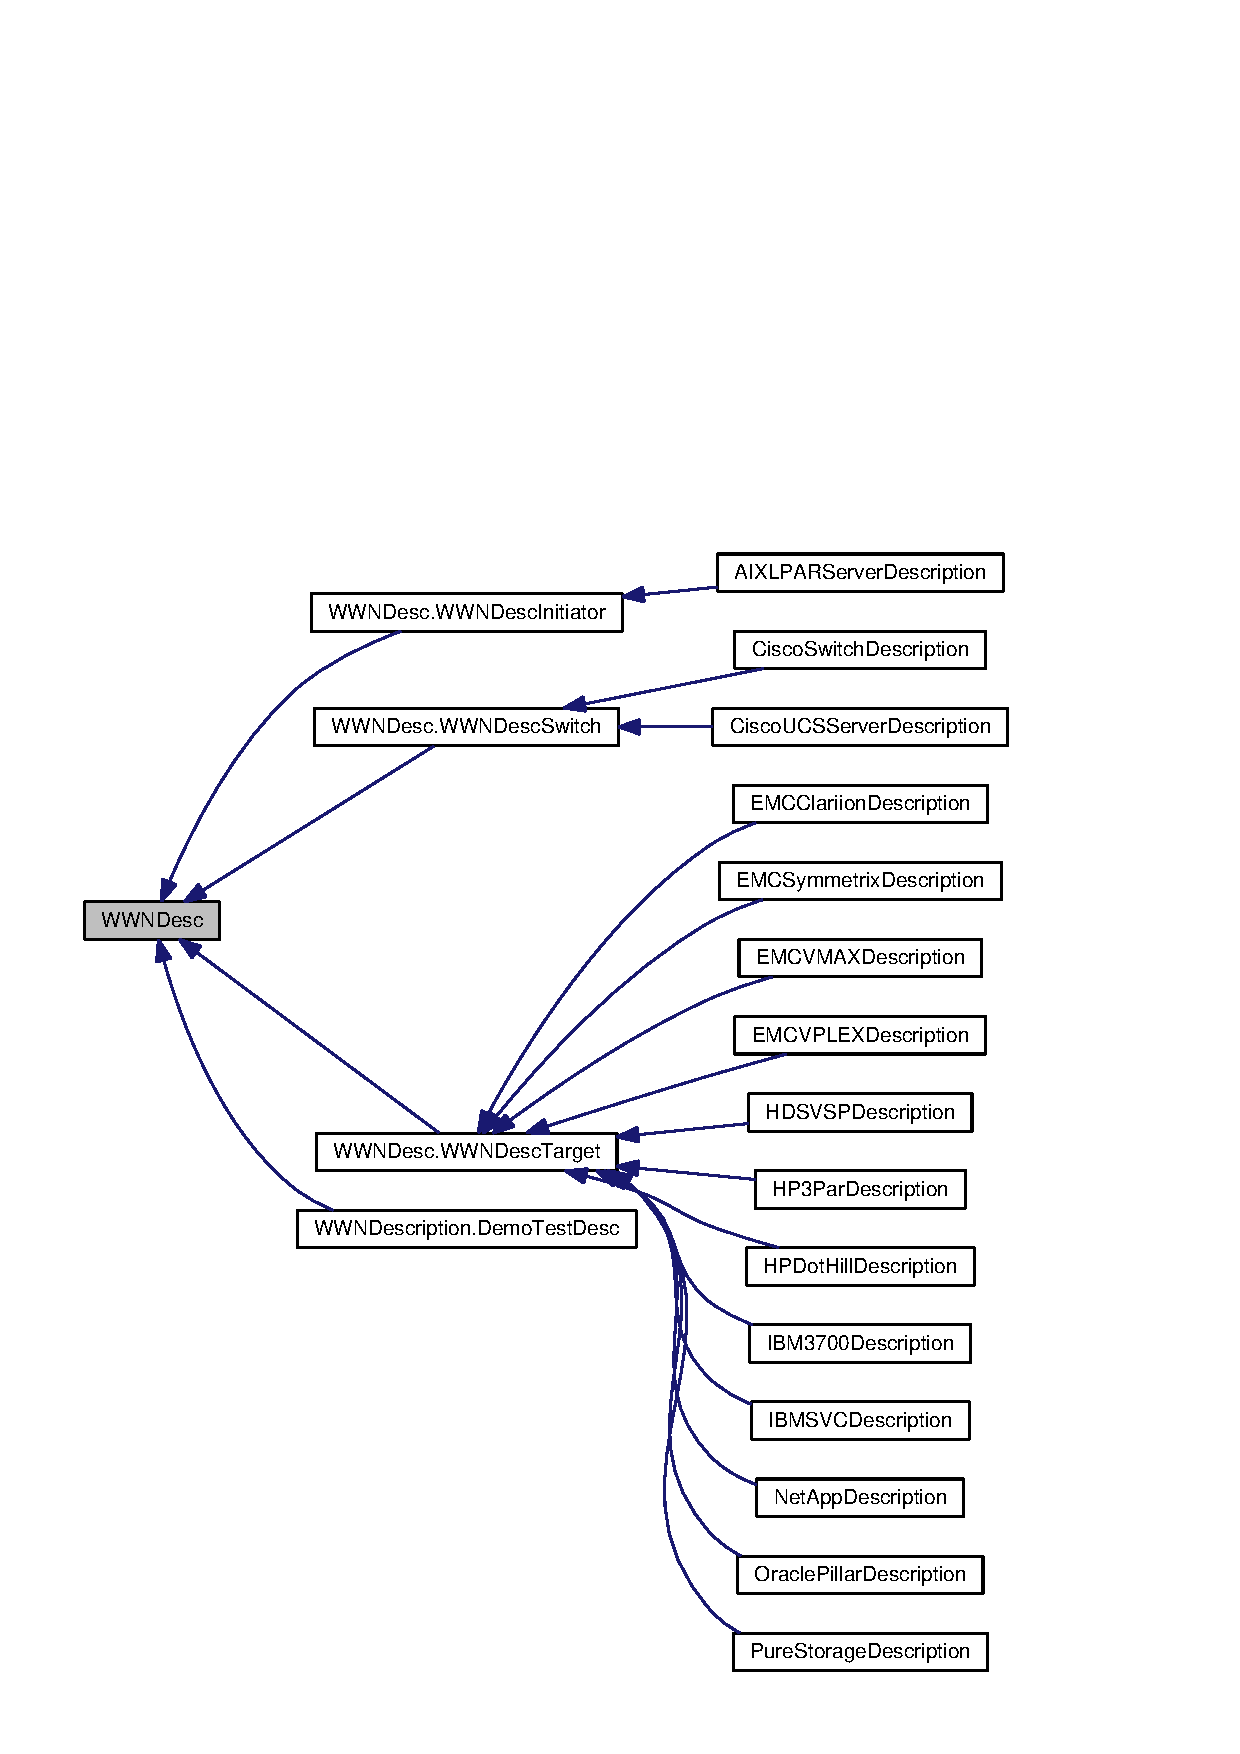
\includegraphics[width=340pt]{classorg_1_1smallfoot_1_1wwn_1_1WWNDesc__inherit__graph}
\end{center}
\end{figure}


Collaboration diagram for W\-W\-N\-Desc\-:\nopagebreak
\begin{figure}[H]
\begin{center}
\leavevmode
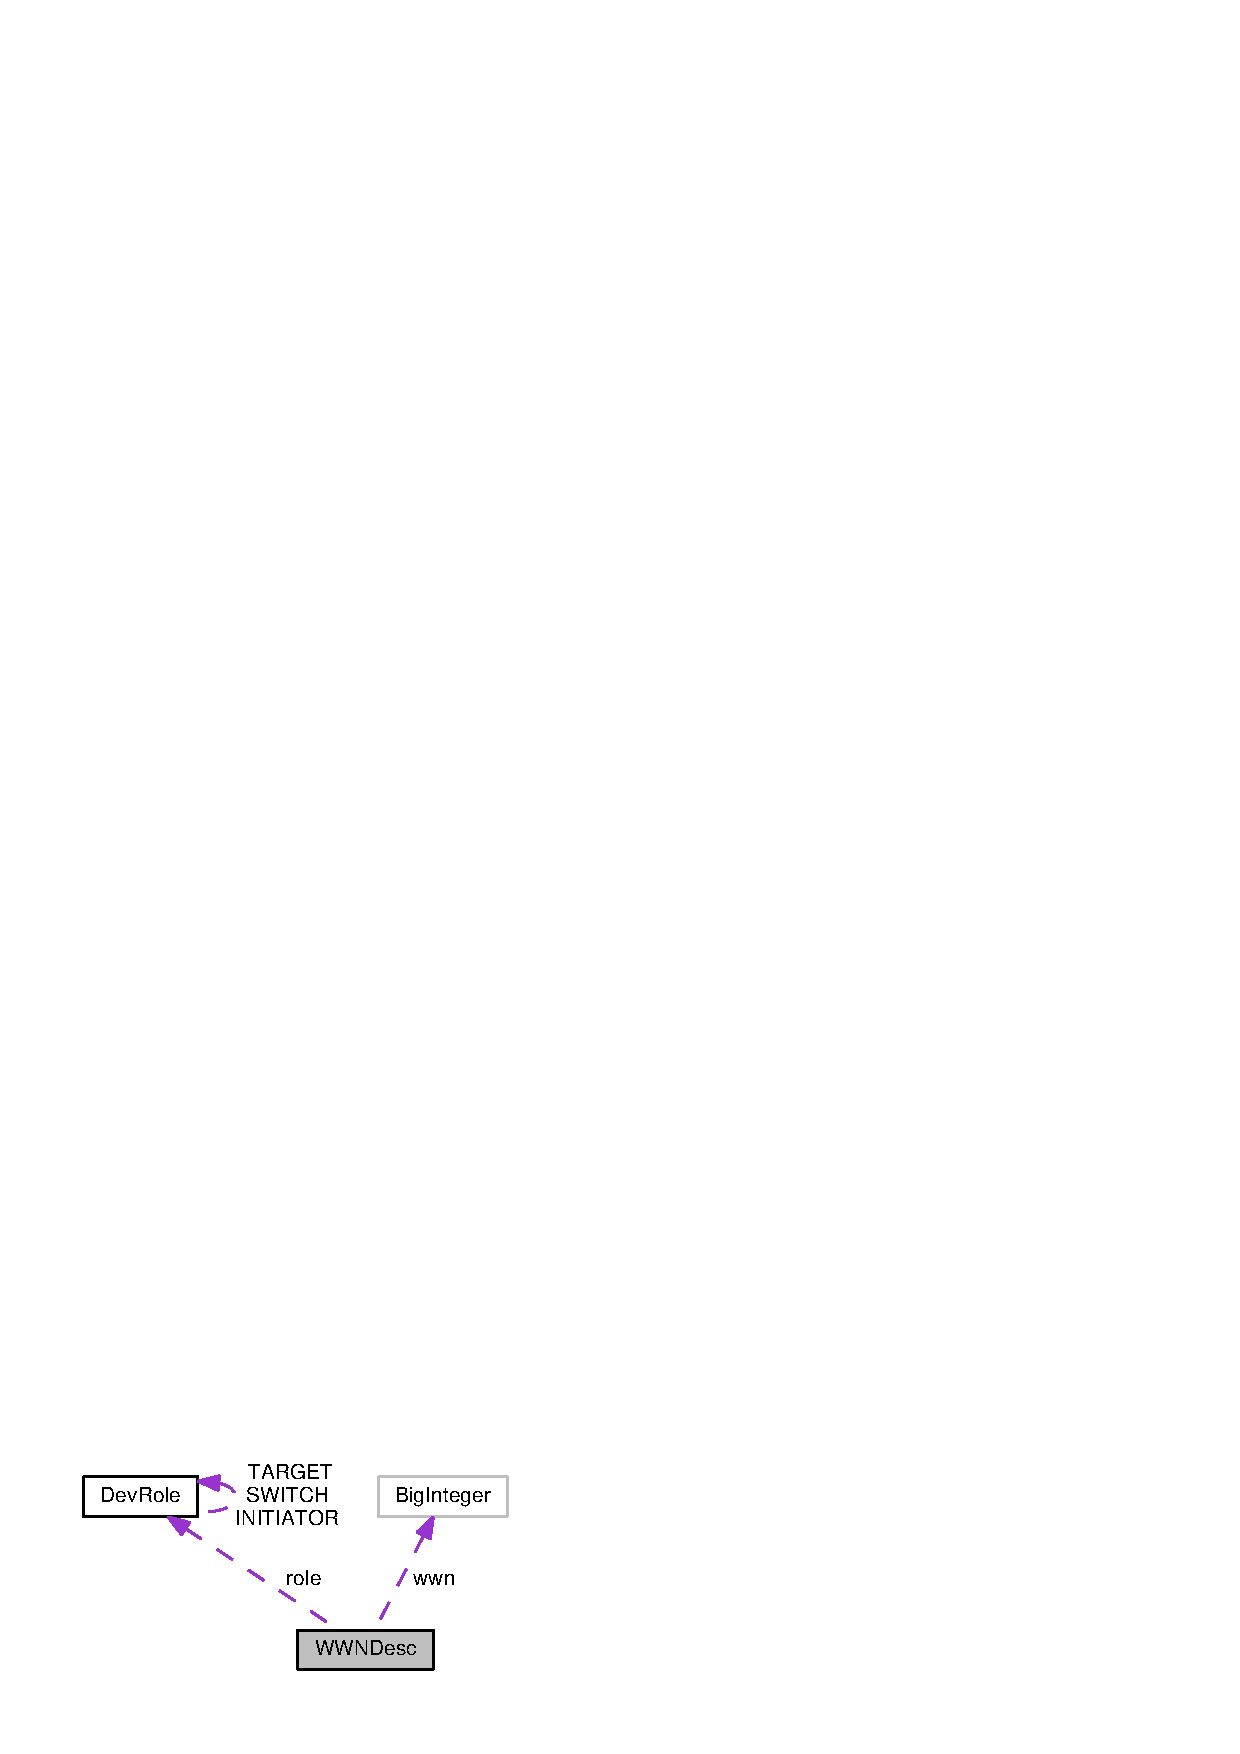
\includegraphics[width=116pt]{classorg_1_1smallfoot_1_1wwn_1_1WWNDesc__coll__graph}
\end{center}
\end{figure}
\subsection*{Public Member Functions}
\begin{DoxyCompactItemize}
\item 
{\bf W\-W\-N\-Desc} (String {\bf wwn})
\begin{DoxyCompactList}\small\item\em create an instance with \doxyref{brief}{p.}{classorg_1_1smallfoot_1_1wwn_1_1WWNDesc_adbebed411e8c47d43338efa3edaa13f8} set to false. \end{DoxyCompactList}\item 
{\bf W\-W\-N\-Desc} (boolean {\bf brief}, String {\bf wwn})
\begin{DoxyCompactList}\small\item\em create an instance with the given W\-W\-N. \end{DoxyCompactList}\item 
String {\bf to\-String} ()
\begin{DoxyCompactList}\small\item\em describe the W\-W\-N\-: produce a short (shorter if this.\-brief = true) description suitable for use as an alias for this W\-W\-N \end{DoxyCompactList}\end{DoxyCompactItemize}
\subsection*{Protected Attributes}
\begin{DoxyCompactItemize}
\item 
boolean {\bf brief}
\begin{DoxyCompactList}\small\item\em whether a more brief output should be offered in \doxyref{to\-String()}{p.}{classorg_1_1smallfoot_1_1wwn_1_1WWNDesc_ad146fa8579a5f8a876c4688cc5a68520} (ie the difference between \char`\"{}\-V\-Max-\/\-H\-K192601234-\/12g\-B\char`\"{} and \char`\"{}\-V\-Max-\/1234-\/12g\-B\char`\"{}) . \end{DoxyCompactList}\item 
Big\-Integer {\bf wwn}\label{classorg_1_1smallfoot_1_1wwn_1_1WWNDesc_aa6eeb40b2983b06aec48b79024fdecea}

\begin{DoxyCompactList}\small\item\em the W\-W\-N that the instance tried to describe \end{DoxyCompactList}\end{DoxyCompactItemize}


\subsection{Detailed Description}
\doxyref{W\-W\-N\-Desc}{p.}{classorg_1_1smallfoot_1_1wwn_1_1WWNDesc} is the basic generic class from which each vendor-\/specific pattern is built upon; similar to an abstract parent but populated methods. 

Definition at line 19 of file W\-W\-N\-Desc.\-java.



\subsection{Constructor \& Destructor Documentation}
\index{org\-::smallfoot\-::wwn\-::\-W\-W\-N\-Desc@{org\-::smallfoot\-::wwn\-::\-W\-W\-N\-Desc}!W\-W\-N\-Desc@{W\-W\-N\-Desc}}
\index{W\-W\-N\-Desc@{W\-W\-N\-Desc}!org::smallfoot::wwn::WWNDesc@{org\-::smallfoot\-::wwn\-::\-W\-W\-N\-Desc}}
\subsubsection[{W\-W\-N\-Desc}]{\setlength{\rightskip}{0pt plus 5cm}{\bf W\-W\-N\-Desc} (
\begin{DoxyParamCaption}
\item[{String}]{wwn}
\end{DoxyParamCaption}
)\hspace{0.3cm}{\ttfamily [inline]}}\label{classorg_1_1smallfoot_1_1wwn_1_1WWNDesc_ade15e20276ee2abd521abb251e61c297}


create an instance with \doxyref{brief}{p.}{classorg_1_1smallfoot_1_1wwn_1_1WWNDesc_adbebed411e8c47d43338efa3edaa13f8} set to false. 

This is a convenience function to support the older constructor model


\begin{DoxyExceptions}{Exceptions}
{\em java.\-lang.\-Null\-Pointer\-Exception} & if the given wwn is null\\
\hline
\end{DoxyExceptions}

\begin{DoxyParams}{Parameters}
{\em wwn} & the W\-W\-N to evaluate and describe \\
\hline
\end{DoxyParams}


Definition at line 31 of file W\-W\-N\-Desc.\-java.



References W\-W\-N\-Desc.\-wwn.

\index{org\-::smallfoot\-::wwn\-::\-W\-W\-N\-Desc@{org\-::smallfoot\-::wwn\-::\-W\-W\-N\-Desc}!W\-W\-N\-Desc@{W\-W\-N\-Desc}}
\index{W\-W\-N\-Desc@{W\-W\-N\-Desc}!org::smallfoot::wwn::WWNDesc@{org\-::smallfoot\-::wwn\-::\-W\-W\-N\-Desc}}
\subsubsection[{W\-W\-N\-Desc}]{\setlength{\rightskip}{0pt plus 5cm}{\bf W\-W\-N\-Desc} (
\begin{DoxyParamCaption}
\item[{boolean}]{brief, }
\item[{String}]{wwn}
\end{DoxyParamCaption}
)\hspace{0.3cm}{\ttfamily [inline]}}\label{classorg_1_1smallfoot_1_1wwn_1_1WWNDesc_a2493316b54bd042475e268e01c2d33af}


create an instance with the given W\-W\-N. 

Values given to the constructor are simply copied to internal variables for later use


\begin{DoxyExceptions}{Exceptions}
{\em java.\-lang.\-Null\-Pointer\-Exception} & if the given wwn is null\\
\hline
\end{DoxyExceptions}

\begin{DoxyParams}{Parameters}
{\em brief} & whether an abbreviated description is requested \\
\hline
{\em wwn} & the W\-W\-N to evaluate and describe \\
\hline
\end{DoxyParams}


Definition at line 43 of file W\-W\-N\-Desc.\-java.



References W\-W\-N\-Desc.\-brief.



\subsection{Member Function Documentation}
\index{org\-::smallfoot\-::wwn\-::\-W\-W\-N\-Desc@{org\-::smallfoot\-::wwn\-::\-W\-W\-N\-Desc}!to\-String@{to\-String}}
\index{to\-String@{to\-String}!org::smallfoot::wwn::WWNDesc@{org\-::smallfoot\-::wwn\-::\-W\-W\-N\-Desc}}
\subsubsection[{to\-String}]{\setlength{\rightskip}{0pt plus 5cm}String to\-String (
\begin{DoxyParamCaption}
{}
\end{DoxyParamCaption}
)\hspace{0.3cm}{\ttfamily [inline]}}\label{classorg_1_1smallfoot_1_1wwn_1_1WWNDesc_ad146fa8579a5f8a876c4688cc5a68520}


describe the W\-W\-N\-: produce a short (shorter if this.\-brief = true) description suitable for use as an alias for this W\-W\-N 

\begin{DoxyReturn}{Returns}
the alias for the W\-W\-N constructed form the W\-W\-N bit fields 
\end{DoxyReturn}


Definition at line 55 of file W\-W\-N\-Desc.\-java.



\subsection{Field Documentation}
\index{org\-::smallfoot\-::wwn\-::\-W\-W\-N\-Desc@{org\-::smallfoot\-::wwn\-::\-W\-W\-N\-Desc}!brief@{brief}}
\index{brief@{brief}!org::smallfoot::wwn::WWNDesc@{org\-::smallfoot\-::wwn\-::\-W\-W\-N\-Desc}}
\subsubsection[{brief}]{\setlength{\rightskip}{0pt plus 5cm}boolean brief\hspace{0.3cm}{\ttfamily [protected]}}\label{classorg_1_1smallfoot_1_1wwn_1_1WWNDesc_adbebed411e8c47d43338efa3edaa13f8}


whether a more brief output should be offered in \doxyref{to\-String()}{p.}{classorg_1_1smallfoot_1_1wwn_1_1WWNDesc_ad146fa8579a5f8a876c4688cc5a68520} (ie the difference between \char`\"{}\-V\-Max-\/\-H\-K192601234-\/12g\-B\char`\"{} and \char`\"{}\-V\-Max-\/1234-\/12g\-B\char`\"{}) . 

. the class may choose to ignore this value 

Definition at line 22 of file W\-W\-N\-Desc.\-java.



Referenced by Pure\-Storage\-Description.\-to\-String(), E\-M\-C\-V\-M\-A\-X\-Description.\-to\-String(), E\-M\-C\-V\-P\-L\-E\-X\-Description.\-to\-String(), E\-M\-C\-Symmetrix\-Description.\-to\-String(), H\-D\-S\-V\-S\-P\-Description.\-to\-String(), Net\-App\-Description.\-to\-String(), I\-B\-M\-S\-V\-C\-Description.\-to\-String(), and W\-W\-N\-Desc.\-W\-W\-N\-Desc().



The documentation for this class was generated from the following file\-:\begin{DoxyCompactItemize}
\item 
java/{\bf W\-W\-N\-Desc.\-java}\end{DoxyCompactItemize}

\section{W\+W\+N\+Description Class Reference}
\label{classorg_1_1smallfoot_1_1wwn_1_1WWNDescription}\index{W\+W\+N\+Description@{W\+W\+N\+Description}}


In situations where nicknames simply are not present, but we need descriptors in short-\/order, the \char`\"{}-\/-\/wwn=\char`\"{} or \char`\"{}-\/w\char`\"{} ooption can be used to get a description of what the most likely Nickname would be.  


\subsection*{Data Structures}
\begin{DoxyCompactItemize}
\item 
class {\bf Demo\+Test\+Desc}
\begin{DoxyCompactList}\small\item\em test case\+: this matches a single item known to exist in the Demo Database \end{DoxyCompactList}\end{DoxyCompactItemize}
\subsection*{Public Member Functions}
\begin{DoxyCompactItemize}
\item 
{\bf W\+W\+N\+Desc} {\bf get\+W\+W\+N\+Descriptor} (String val)
\begin{DoxyCompactList}\small\item\em Iterates \doxyref{W\+W\+N\+Description}{p.}{classorg_1_1smallfoot_1_1wwn_1_1WWNDescription} decendents looking for which will accept responsibility, and if so, returns the instance it generates as a descriptor. \end{DoxyCompactList}\item 
{\bf W\+W\+N\+Desc} {\bf get\+W\+W\+N\+Descriptor} (String val, boolean provide\+Base)
\begin{DoxyCompactList}\small\item\em Iterates \doxyref{W\+W\+N\+Description}{p.}{classorg_1_1smallfoot_1_1wwn_1_1WWNDescription} decendents looking for which will accept responsibility, and if so, returns the instance it generates as a descriptor. \end{DoxyCompactList}\item 
{\bf W\+W\+N\+Desc} {\bf get\+W\+W\+N\+Descriptor} (String val, boolean provide\+Base, {\bf Dev\+Role} role)
\begin{DoxyCompactList}\small\item\em Iterates \doxyref{W\+W\+N\+Description}{p.}{classorg_1_1smallfoot_1_1wwn_1_1WWNDescription} decendents looking for which will accept responsibility, and if so, returns the instance it generates as a descriptor. \end{DoxyCompactList}\item 
{\bf W\+W\+N\+Desc} {\bf get\+W\+W\+N\+Descriptor} (String val, boolean provide\+Base, int role)
\begin{DoxyCompactList}\small\item\em Iterates \doxyref{W\+W\+N\+Description}{p.}{classorg_1_1smallfoot_1_1wwn_1_1WWNDescription} decendents looking for which will accept responsibility, and if so, returns the instance it generates as a descriptor. \end{DoxyCompactList}\item 
void {\bf usage} (String proc)
\begin{DoxyCompactList}\small\item\em usage messages are useful to those of us with short memories as well (hey, I just need to add swap!) \end{DoxyCompactList}\end{DoxyCompactItemize}
\subsection*{Static Public Member Functions}
\begin{DoxyCompactItemize}
\item 
static void {\bf main} (String args[$\,$])
\begin{DoxyCompactList}\small\item\em Main function, as you can tell. \end{DoxyCompactList}\end{DoxyCompactItemize}
\subsection*{Data Fields}
\begin{DoxyCompactItemize}
\item 
boolean {\bf brief\+W\+W\+N\+Estimate} = false
\begin{DoxyCompactList}\small\item\em setting to \char`\"{}true\char`\"{} via the \char`\"{}-\/-\/briefestimate\char`\"{} commandline causes all descriptions later requested in \doxyref{get\+W\+W\+N\+Descriptor(\+String)}{p.}{classorg_1_1smallfoot_1_1wwn_1_1WWNDescription_a44589ea01f3c2e5a8fbe84cb249ec404} to be \char`\"{}brief\char`\"{} (more concise) \end{DoxyCompactList}\end{DoxyCompactItemize}


\subsection{Detailed Description}
In situations where nicknames simply are not present, but we need descriptors in short-\/order, the \char`\"{}-\/-\/wwn=\char`\"{} or \char`\"{}-\/w\char`\"{} ooption can be used to get a description of what the most likely Nickname would be. 

For example, \char`\"{}java -\/jar wwndesc.\+jar -\/w 5006048\+A\+C\+C\+C86\+A32\char`\"{} results in \char`\"{}\+Symm-\/182500953-\/05b\+A\char`\"{} matching {\tt http\+://www.\+emcstorageinfo.\+com/2007/08/how-\/to-\/decode-\/symmetrix-\/world-\/wide.\+html} Note that --briefestimate and --nobriefestimate configure for more brief estimate/suggested nicknames\subsection{Examples}\label{classorg_1_1smallfoot_1_1wwn_1_1WWNDescription_Examples}
java -\/jar vict.\+jar --wwn 500610601234567

java -\/jar vict.\+jar --briefestimate --wwn 500610601234567

java -\/jar vict.\+jar --nobriefestimate --wwn 5000097301234564\subsection{Issues}\label{classorg_1_1smallfoot_1_1wwn_1_1WWNDescription_Known}


Definition at line 29 of file W\+W\+N\+Description.\+java.



\subsection{Member Function Documentation}
\index{org\+::smallfoot\+::wwn\+::\+W\+W\+N\+Description@{org\+::smallfoot\+::wwn\+::\+W\+W\+N\+Description}!get\+W\+W\+N\+Descriptor@{get\+W\+W\+N\+Descriptor}}
\index{get\+W\+W\+N\+Descriptor@{get\+W\+W\+N\+Descriptor}!org\+::smallfoot\+::wwn\+::\+W\+W\+N\+Description@{org\+::smallfoot\+::wwn\+::\+W\+W\+N\+Description}}
\subsubsection[{get\+W\+W\+N\+Descriptor}]{\setlength{\rightskip}{0pt plus 5cm}{\bf W\+W\+N\+Desc} get\+W\+W\+N\+Descriptor (
\begin{DoxyParamCaption}
\item[{String}]{val}
\end{DoxyParamCaption}
)\hspace{0.3cm}{\ttfamily [inline]}}\label{classorg_1_1smallfoot_1_1wwn_1_1WWNDescription_a44589ea01f3c2e5a8fbe84cb249ec404}


Iterates \doxyref{W\+W\+N\+Description}{p.}{classorg_1_1smallfoot_1_1wwn_1_1WWNDescription} decendents looking for which will accept responsibility, and if so, returns the instance it generates as a descriptor. 

\begin{DoxyReturn}{Returns}
new instance of \doxyref{W\+W\+N\+Desc}{p.}{classorg_1_1smallfoot_1_1wwn_1_1WWNDesc} descendent, or null if no descendents accept responsibility to describe or provide an alias for that W\+W\+N
\end{DoxyReturn}

\begin{DoxyParams}{Parameters}
{\em val} & W\+W\+N to check \\
\hline
\end{DoxyParams}


Definition at line 62 of file W\+W\+N\+Description.\+java.



Referenced by W\+W\+N\+Description.\+get\+W\+W\+N\+Descriptor(), and W\+W\+N\+Description.\+main().

\index{org\+::smallfoot\+::wwn\+::\+W\+W\+N\+Description@{org\+::smallfoot\+::wwn\+::\+W\+W\+N\+Description}!get\+W\+W\+N\+Descriptor@{get\+W\+W\+N\+Descriptor}}
\index{get\+W\+W\+N\+Descriptor@{get\+W\+W\+N\+Descriptor}!org\+::smallfoot\+::wwn\+::\+W\+W\+N\+Description@{org\+::smallfoot\+::wwn\+::\+W\+W\+N\+Description}}
\subsubsection[{get\+W\+W\+N\+Descriptor}]{\setlength{\rightskip}{0pt plus 5cm}{\bf W\+W\+N\+Desc} get\+W\+W\+N\+Descriptor (
\begin{DoxyParamCaption}
\item[{String}]{val, }
\item[{boolean}]{provide\+Base}
\end{DoxyParamCaption}
)\hspace{0.3cm}{\ttfamily [inline]}}\label{classorg_1_1smallfoot_1_1wwn_1_1WWNDescription_ad107e09f44b93a618bae90e3b32e96f8}


Iterates \doxyref{W\+W\+N\+Description}{p.}{classorg_1_1smallfoot_1_1wwn_1_1WWNDescription} decendents looking for which will accept responsibility, and if so, returns the instance it generates as a descriptor. 

\begin{DoxyReturn}{Returns}
new instance of \doxyref{W\+W\+N\+Desc}{p.}{classorg_1_1smallfoot_1_1wwn_1_1WWNDesc} descendent, or null if no descendents accept responsibility to describe or provide an alias for that W\+W\+N
\end{DoxyReturn}

\begin{DoxyParams}{Parameters}
{\em val} & W\+W\+N to check \\
\hline
{\em provide\+Base} & whether to provide a bogus \doxyref{W\+W\+N\+Desc}{p.}{classorg_1_1smallfoot_1_1wwn_1_1WWNDesc} instance rather than a null \\
\hline
\end{DoxyParams}


Definition at line 75 of file W\+W\+N\+Description.\+java.



References W\+W\+N\+Description.\+get\+W\+W\+N\+Descriptor().



Here is the call graph for this function\+:\nopagebreak
\begin{figure}[H]
\begin{center}
\leavevmode
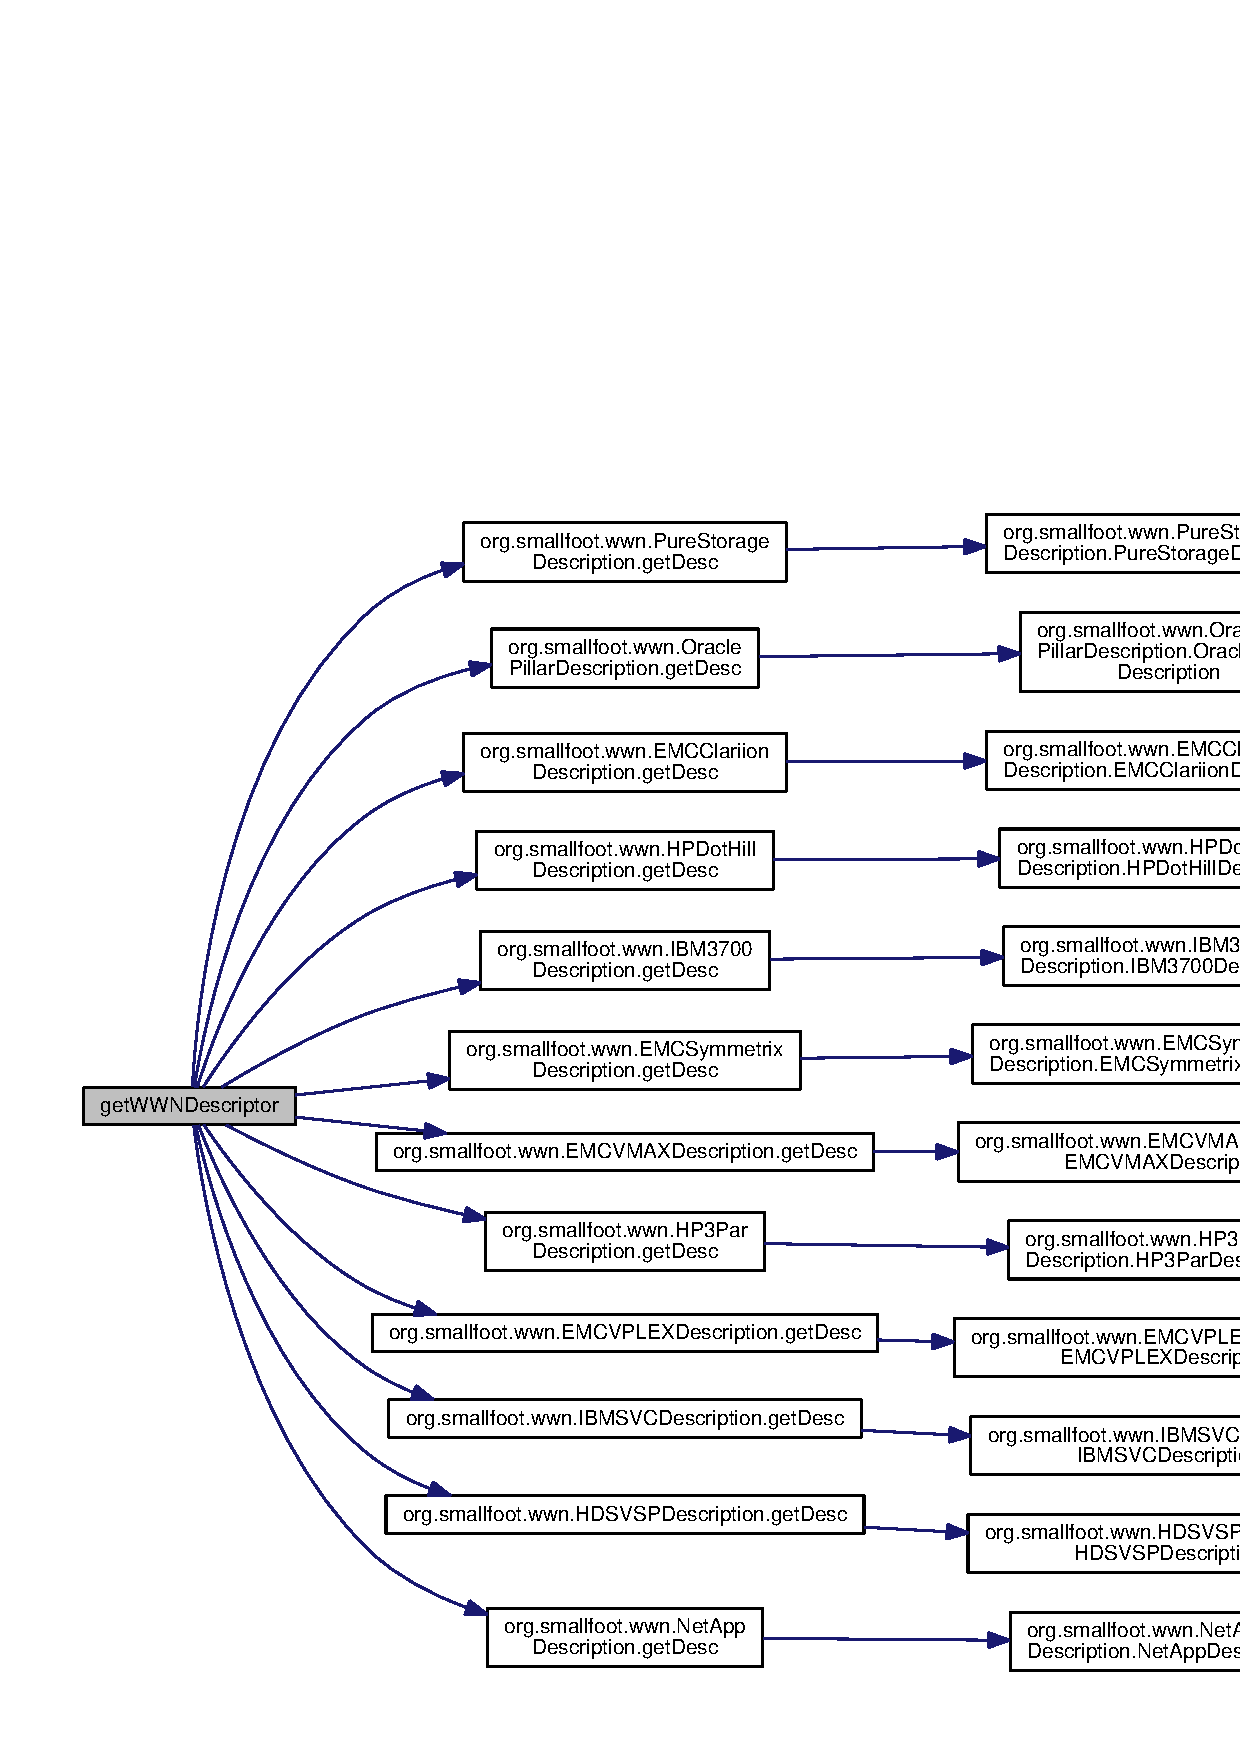
\includegraphics[width=284pt]{classorg_1_1smallfoot_1_1wwn_1_1WWNDescription_ad107e09f44b93a618bae90e3b32e96f8_cgraph}
\end{center}
\end{figure}


\index{org\+::smallfoot\+::wwn\+::\+W\+W\+N\+Description@{org\+::smallfoot\+::wwn\+::\+W\+W\+N\+Description}!get\+W\+W\+N\+Descriptor@{get\+W\+W\+N\+Descriptor}}
\index{get\+W\+W\+N\+Descriptor@{get\+W\+W\+N\+Descriptor}!org\+::smallfoot\+::wwn\+::\+W\+W\+N\+Description@{org\+::smallfoot\+::wwn\+::\+W\+W\+N\+Description}}
\subsubsection[{get\+W\+W\+N\+Descriptor}]{\setlength{\rightskip}{0pt plus 5cm}{\bf W\+W\+N\+Desc} get\+W\+W\+N\+Descriptor (
\begin{DoxyParamCaption}
\item[{String}]{val, }
\item[{boolean}]{provide\+Base, }
\item[{{\bf Dev\+Role}}]{role}
\end{DoxyParamCaption}
)\hspace{0.3cm}{\ttfamily [inline]}}\label{classorg_1_1smallfoot_1_1wwn_1_1WWNDescription_a75059cc51be3b90691caaad2ea2b96c6}


Iterates \doxyref{W\+W\+N\+Description}{p.}{classorg_1_1smallfoot_1_1wwn_1_1WWNDescription} decendents looking for which will accept responsibility, and if so, returns the instance it generates as a descriptor. 

\begin{DoxyReturn}{Returns}
new instance of \doxyref{W\+W\+N\+Desc}{p.}{classorg_1_1smallfoot_1_1wwn_1_1WWNDesc} descendent, or null if no descendents accept responsibility to describe or provide an alias for that W\+W\+N
\end{DoxyReturn}

\begin{DoxyParams}{Parameters}
{\em val} & W\+W\+N to check \\
\hline
{\em provide\+Base} & whether to provide a bogus \doxyref{W\+W\+N\+Desc}{p.}{classorg_1_1smallfoot_1_1wwn_1_1WWNDesc} instance rather than a null\\
\hline
{\em role} & \doxyref{Dev\+Role}{p.}{classorg_1_1smallfoot_1_1wwn_1_1DevRole} to check for \\
\hline
\end{DoxyParams}


Definition at line 84 of file W\+W\+N\+Description.\+java.



References W\+W\+N\+Description.\+get\+W\+W\+N\+Descriptor(), and Dev\+Role.\+value.



Here is the call graph for this function\+:\nopagebreak
\begin{figure}[H]
\begin{center}
\leavevmode
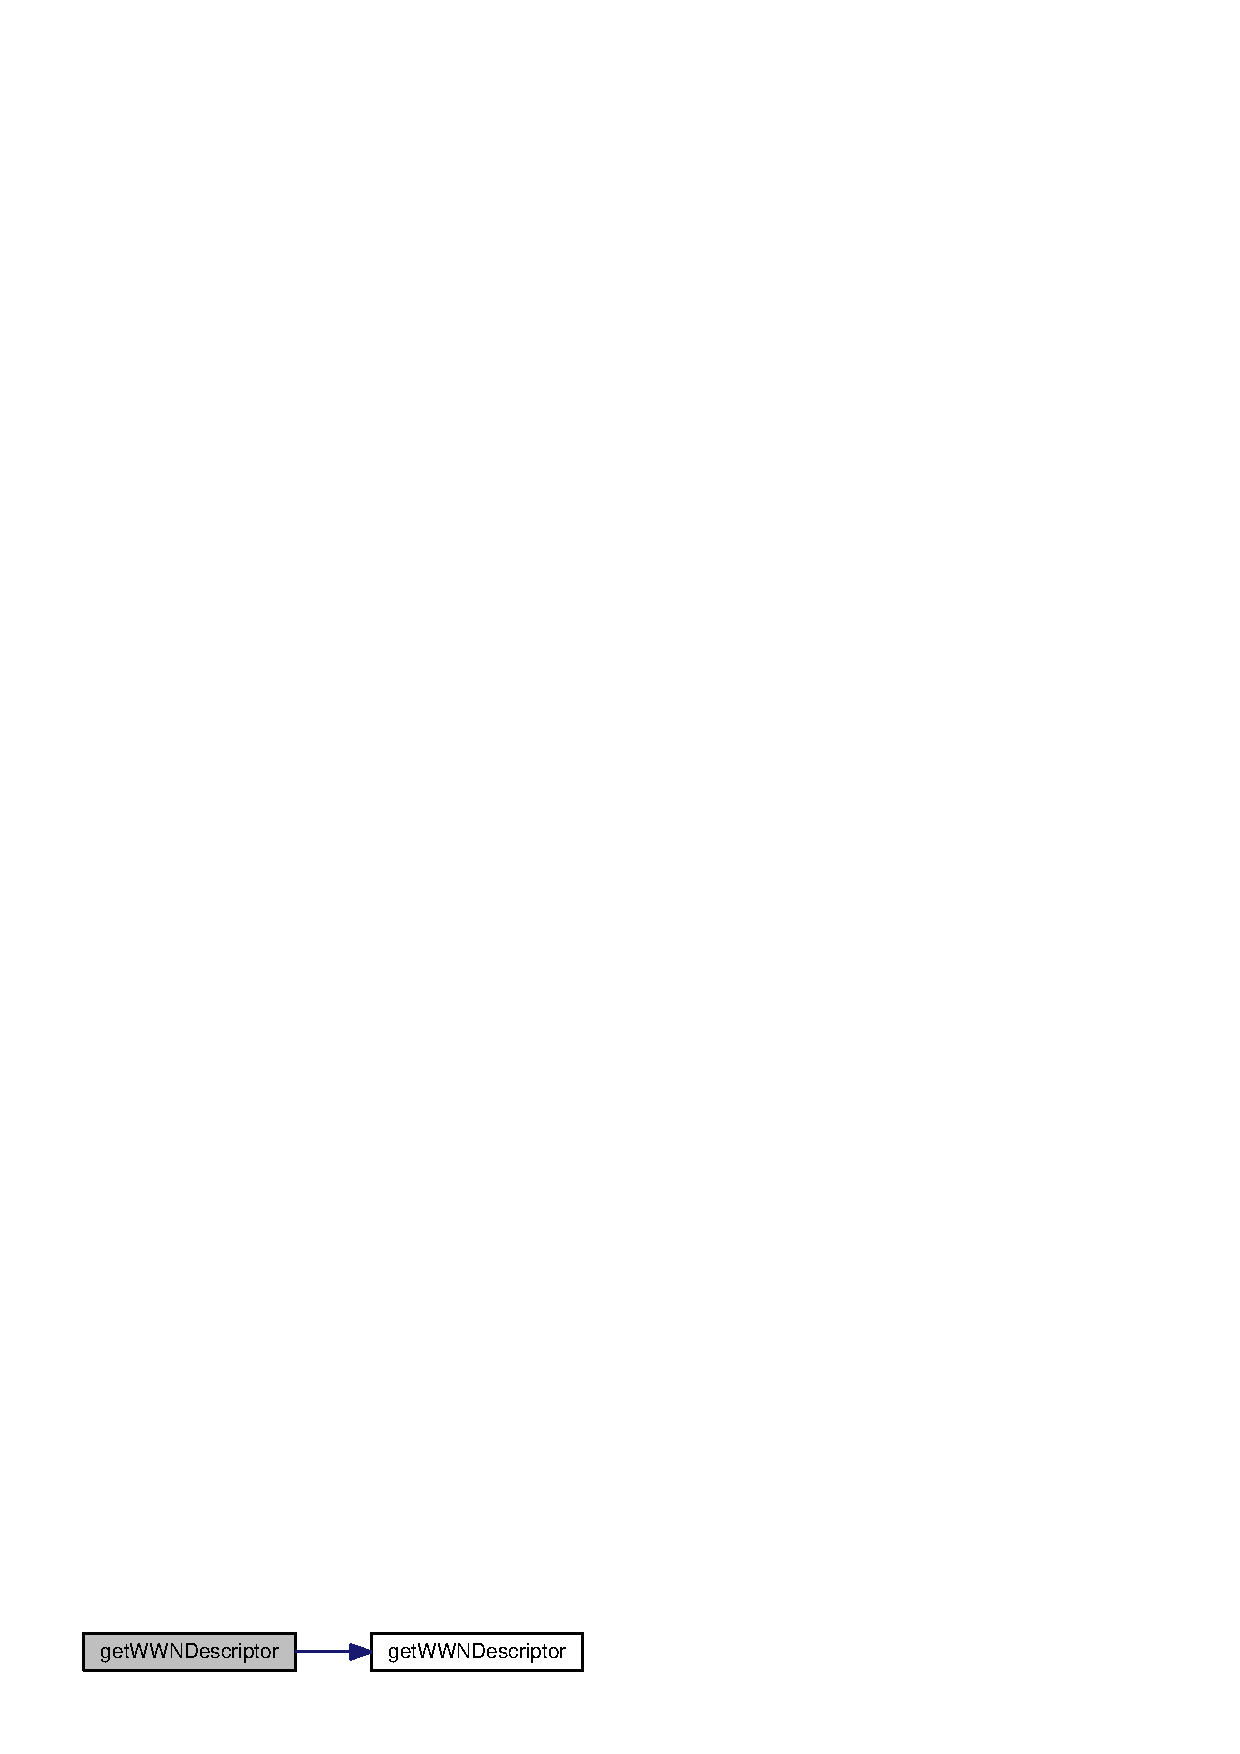
\includegraphics[width=284pt]{classorg_1_1smallfoot_1_1wwn_1_1WWNDescription_a75059cc51be3b90691caaad2ea2b96c6_cgraph}
\end{center}
\end{figure}


\index{org\+::smallfoot\+::wwn\+::\+W\+W\+N\+Description@{org\+::smallfoot\+::wwn\+::\+W\+W\+N\+Description}!get\+W\+W\+N\+Descriptor@{get\+W\+W\+N\+Descriptor}}
\index{get\+W\+W\+N\+Descriptor@{get\+W\+W\+N\+Descriptor}!org\+::smallfoot\+::wwn\+::\+W\+W\+N\+Description@{org\+::smallfoot\+::wwn\+::\+W\+W\+N\+Description}}
\subsubsection[{get\+W\+W\+N\+Descriptor}]{\setlength{\rightskip}{0pt plus 5cm}{\bf W\+W\+N\+Desc} get\+W\+W\+N\+Descriptor (
\begin{DoxyParamCaption}
\item[{String}]{val, }
\item[{boolean}]{provide\+Base, }
\item[{int}]{role}
\end{DoxyParamCaption}
)\hspace{0.3cm}{\ttfamily [inline]}}\label{classorg_1_1smallfoot_1_1wwn_1_1WWNDescription_a096d21a419b9a081abec2e2fcaf6eb5d}


Iterates \doxyref{W\+W\+N\+Description}{p.}{classorg_1_1smallfoot_1_1wwn_1_1WWNDescription} decendents looking for which will accept responsibility, and if so, returns the instance it generates as a descriptor. 

\begin{DoxyReturn}{Returns}
new instance of \doxyref{W\+W\+N\+Desc}{p.}{classorg_1_1smallfoot_1_1wwn_1_1WWNDesc} descendent, or null if no descendents accept responsibility to describe or provide an alias for that W\+W\+N
\end{DoxyReturn}

\begin{DoxyParams}{Parameters}
{\em val} & W\+W\+N to check \\
\hline
{\em provide\+Base} & whether to provide a bogus \doxyref{W\+W\+N\+Desc}{p.}{classorg_1_1smallfoot_1_1wwn_1_1WWNDesc} instance rather than a null\\
\hline
{\em role} & \doxyref{Dev\+Role}{p.}{classorg_1_1smallfoot_1_1wwn_1_1DevRole} to check for \\
\hline
\end{DoxyParams}


Definition at line 91 of file W\+W\+N\+Description.\+java.



References Pure\+Storage\+Description.\+get\+Desc(), Cisco\+Switch\+Description.\+get\+Desc(), A\+I\+X\+L\+P\+A\+R\+Server\+Description.\+get\+Desc(), E\+M\+C\+Clariion\+Description.\+get\+Desc(), Oracle\+Pillar\+Description.\+get\+Desc(), H\+P\+Dot\+Hill\+Description.\+get\+Desc(), Cisco\+U\+C\+S\+Server\+Description.\+get\+Desc(), I\+B\+M\+S\+V\+C\+Description.\+get\+Desc(), I\+B\+M3700\+Description.\+get\+Desc(), E\+M\+C\+Symmetrix\+Description.\+get\+Desc(), E\+M\+C\+V\+P\+L\+E\+X\+Description.\+get\+Desc(), H\+P3\+Par\+Description.\+get\+Desc(), E\+M\+C\+V\+M\+A\+X\+Description.\+get\+Desc(), Net\+App\+Description.\+get\+Desc(), and H\+D\+S\+V\+S\+P\+Description.\+get\+Desc().



Here is the call graph for this function\+:\nopagebreak
\begin{figure}[H]
\begin{center}
\leavevmode
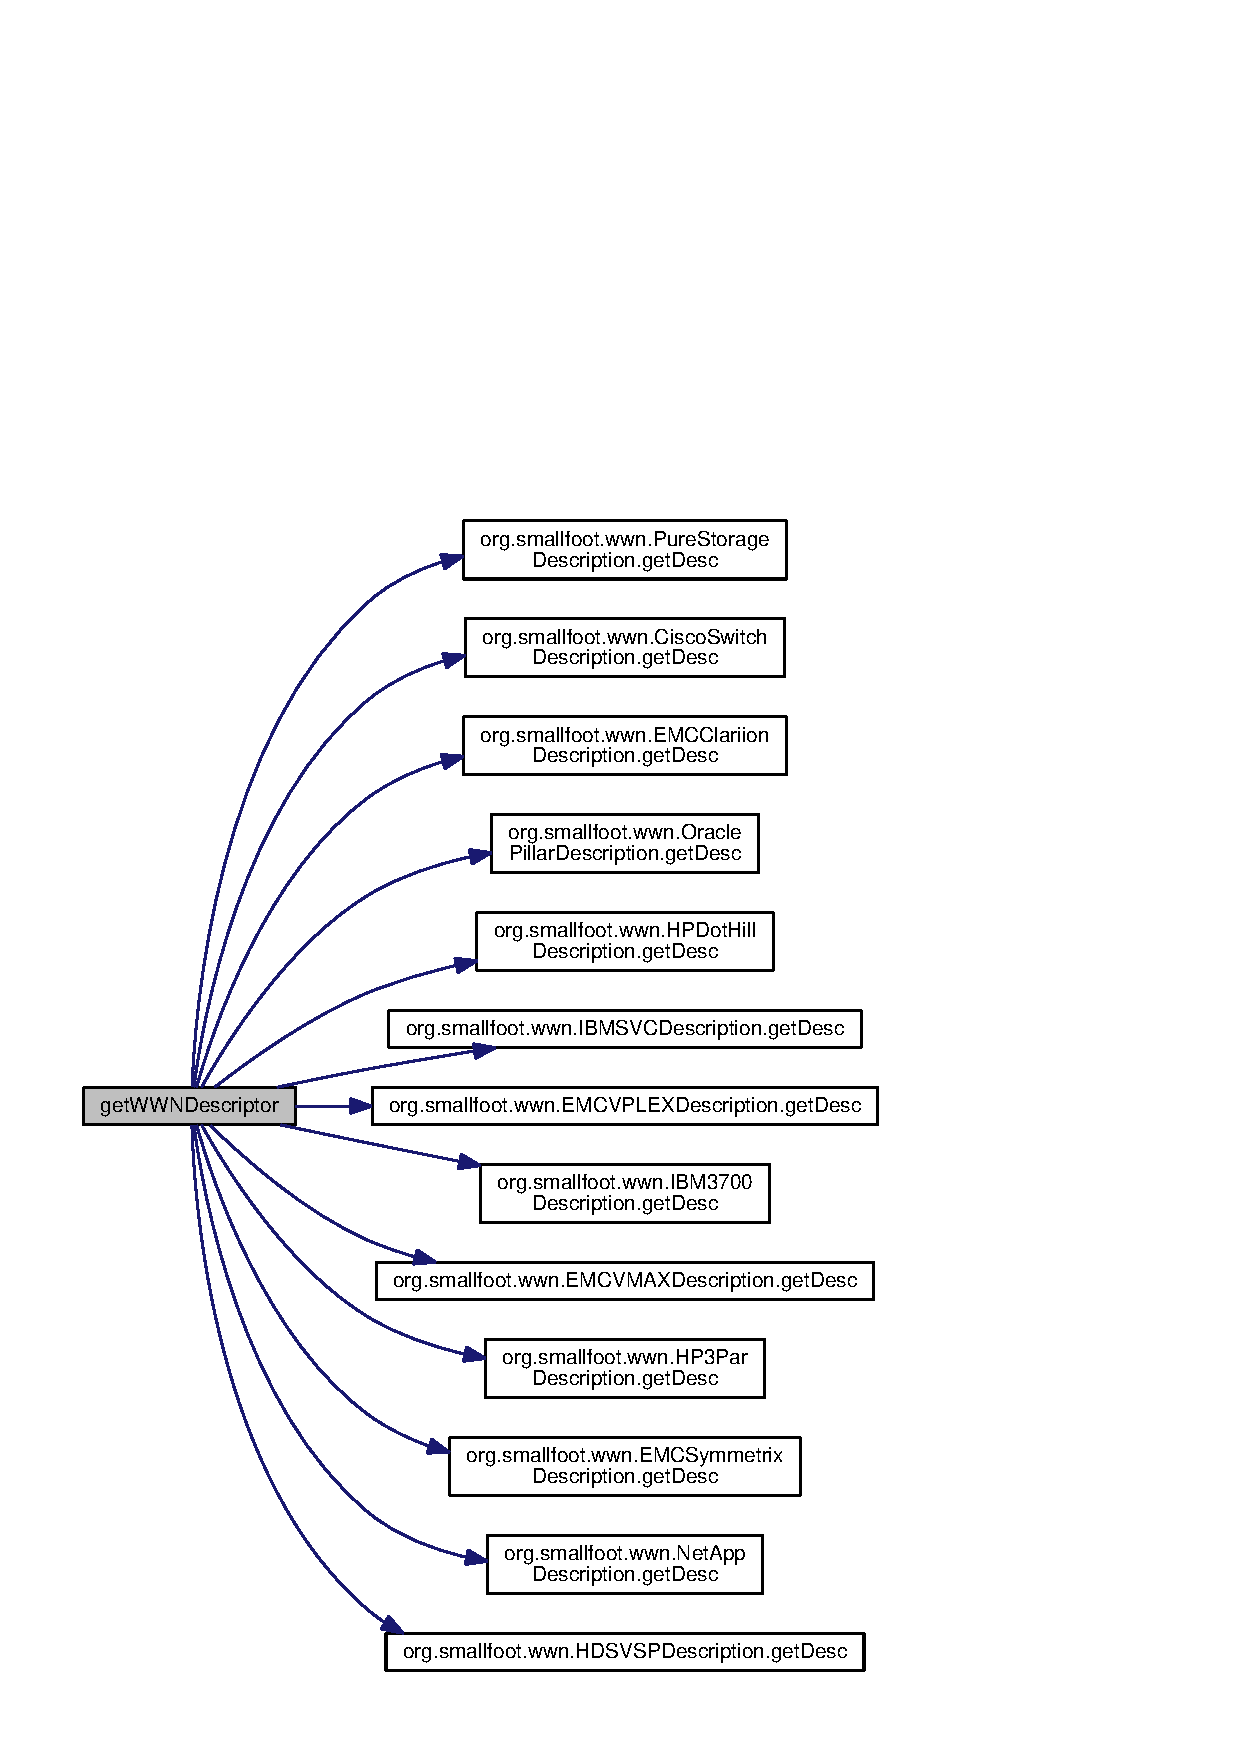
\includegraphics[height=550pt]{classorg_1_1smallfoot_1_1wwn_1_1WWNDescription_a096d21a419b9a081abec2e2fcaf6eb5d_cgraph}
\end{center}
\end{figure}


\index{org\+::smallfoot\+::wwn\+::\+W\+W\+N\+Description@{org\+::smallfoot\+::wwn\+::\+W\+W\+N\+Description}!main@{main}}
\index{main@{main}!org\+::smallfoot\+::wwn\+::\+W\+W\+N\+Description@{org\+::smallfoot\+::wwn\+::\+W\+W\+N\+Description}}
\subsubsection[{main}]{\setlength{\rightskip}{0pt plus 5cm}static void main (
\begin{DoxyParamCaption}
\item[{String}]{args[$\,$]}
\end{DoxyParamCaption}
)\hspace{0.3cm}{\ttfamily [inline]}, {\ttfamily [static]}}\label{classorg_1_1smallfoot_1_1wwn_1_1WWNDescription_a75988cf84fc6ee7a2ebff36e363021aa}


Main function, as you can tell. 

this function merely parses the command-\/line to dispatch actions to the meat of the meal above. I'm using an actual Get\+Opt because, yes, I'm a U\+N\+I\+X/\+C hack, re-\/using 3-\/decades-\/old knowledge, but this also preserves both extensibility and the ability to use longopts in scripts as a way to self-\/document what the tool's doing.

No real intelligence herein except the parse-\/and-\/redirect action.


\begin{DoxyParams}{Parameters}
{\em args} & commandline arguments passed in by the J\+R\+E \\
\hline
\end{DoxyParams}


Definition at line 171 of file W\+W\+N\+Description.\+java.



References W\+W\+N\+Description.\+brief\+W\+W\+N\+Estimate, W\+W\+N\+Desc.\+desc\+Port(), W\+W\+N\+Description.\+get\+W\+W\+N\+Descriptor(), W\+W\+N\+Desc.\+to\+String(), and W\+W\+N\+Description.\+usage().



Here is the call graph for this function\+:\nopagebreak
\begin{figure}[H]
\begin{center}
\leavevmode
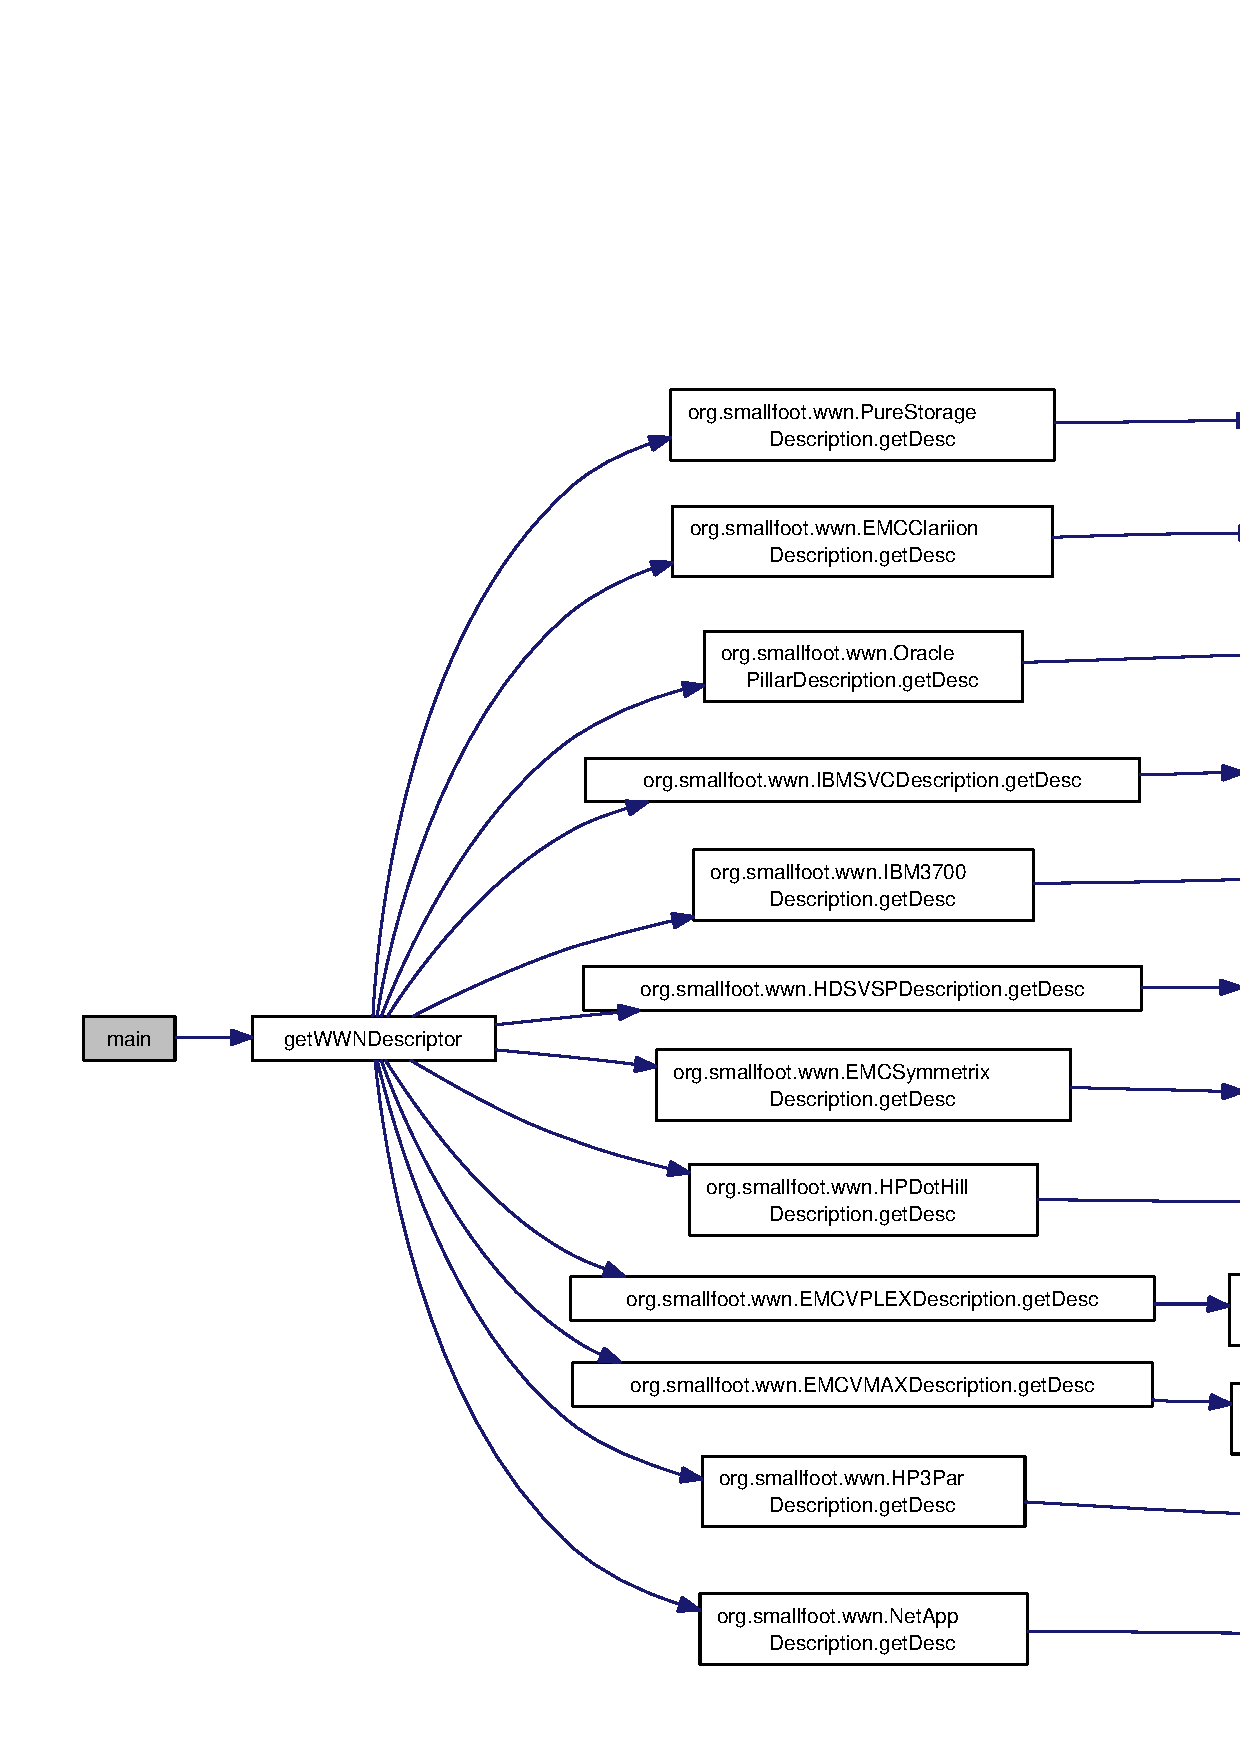
\includegraphics[width=308pt]{classorg_1_1smallfoot_1_1wwn_1_1WWNDescription_a75988cf84fc6ee7a2ebff36e363021aa_cgraph}
\end{center}
\end{figure}


\index{org\+::smallfoot\+::wwn\+::\+W\+W\+N\+Description@{org\+::smallfoot\+::wwn\+::\+W\+W\+N\+Description}!usage@{usage}}
\index{usage@{usage}!org\+::smallfoot\+::wwn\+::\+W\+W\+N\+Description@{org\+::smallfoot\+::wwn\+::\+W\+W\+N\+Description}}
\subsubsection[{usage}]{\setlength{\rightskip}{0pt plus 5cm}void usage (
\begin{DoxyParamCaption}
\item[{String}]{proc}
\end{DoxyParamCaption}
)\hspace{0.3cm}{\ttfamily [inline]}}\label{classorg_1_1smallfoot_1_1wwn_1_1WWNDescription_a65d03ca5cd39f6905d34f7b0aab28f42}


usage messages are useful to those of us with short memories as well (hey, I just need to add swap!) 


\begin{DoxyParams}{Parameters}
{\em proc} & name of the process or program (ie wwndesc) \\
\hline
\end{DoxyParams}


Definition at line 143 of file W\+W\+N\+Description.\+java.



Referenced by W\+W\+N\+Description.\+main().



\subsection{Field Documentation}
\index{org\+::smallfoot\+::wwn\+::\+W\+W\+N\+Description@{org\+::smallfoot\+::wwn\+::\+W\+W\+N\+Description}!brief\+W\+W\+N\+Estimate@{brief\+W\+W\+N\+Estimate}}
\index{brief\+W\+W\+N\+Estimate@{brief\+W\+W\+N\+Estimate}!org\+::smallfoot\+::wwn\+::\+W\+W\+N\+Description@{org\+::smallfoot\+::wwn\+::\+W\+W\+N\+Description}}
\subsubsection[{brief\+W\+W\+N\+Estimate}]{\setlength{\rightskip}{0pt plus 5cm}boolean brief\+W\+W\+N\+Estimate = false}\label{classorg_1_1smallfoot_1_1wwn_1_1WWNDescription_a48cfcc3bfbc4d22cd4ad0fb8c46aeff8}


setting to \char`\"{}true\char`\"{} via the \char`\"{}-\/-\/briefestimate\char`\"{} commandline causes all descriptions later requested in \doxyref{get\+W\+W\+N\+Descriptor(\+String)}{p.}{classorg_1_1smallfoot_1_1wwn_1_1WWNDescription_a44589ea01f3c2e5a8fbe84cb249ec404} to be \char`\"{}brief\char`\"{} (more concise) 

\begin{DoxySeeAlso}{See also}
\doxyref{W\+W\+N\+Desc\+::to\+String()}{p.}{classorg_1_1smallfoot_1_1wwn_1_1WWNDesc_ad146fa8579a5f8a876c4688cc5a68520} 
\end{DoxySeeAlso}


Definition at line 31 of file W\+W\+N\+Description.\+java.



Referenced by W\+W\+N\+Description.\+main().



The documentation for this class was generated from the following file\+:\begin{DoxyCompactItemize}
\item 
java/{\bf W\+W\+N\+Description.\+java}\end{DoxyCompactItemize}

\chapter{File Documentation}
\section{htdocs/\-R\-E\-A\-D\-M\-E.dox \-File \-Reference}
\label{README_8dox}\index{htdocs/\-R\-E\-A\-D\-M\-E.\-dox@{htdocs/\-R\-E\-A\-D\-M\-E.\-dox}}


\subsection{\-Detailed \-Description}


\-Definition in file {\bf \-R\-E\-A\-D\-M\-E.\-dox}.


\section{java/\+E\+M\+C\+Clariion\+Description.java File Reference}
\label{EMCClariionDescription_8java}\index{java/\+E\+M\+C\+Clariion\+Description.\+java@{java/\+E\+M\+C\+Clariion\+Description.\+java}}
\subsection*{Data Structures}
\begin{DoxyCompactItemize}
\item 
class {\bf E\+M\+C\+Clariion\+Description}
\begin{DoxyCompactList}\small\item\em \doxyref{E\+M\+C\+Clariion\+Description}{p.}{classorg_1_1smallfoot_1_1wwn_1_1EMCClariionDescription} (ie C\+L-\/01234567-\/\+S\+P\+B1) describes the serial and C\+L of a Clariion; E\+M\+C doesn\textquotesingle{}t seem to include any additional data in the W\+W\+P\+N. \end{DoxyCompactList}\end{DoxyCompactItemize}

\section{java/\-E\-M\-C\-Symmetrix\-Description.java File Reference}
\label{EMCSymmetrixDescription_8java}\index{java/\-E\-M\-C\-Symmetrix\-Description.\-java@{java/\-E\-M\-C\-Symmetrix\-Description.\-java}}
\subsection*{Data Structures}
\begin{DoxyCompactItemize}
\item 
class {\bf E\-M\-C\-Symmetrix\-Description}
\begin{DoxyCompactList}\small\item\em \doxyref{E\-M\-C\-Symmetrix\-Description}{p.}{classorg_1_1smallfoot_1_1wwn_1_1EMCSymmetrixDescription} (ie Symm-\/187900328-\/03d\-B or Symm-\/0328-\/03d\-B) breaks out the serial and F\-A port from the W\-W\-P\-N. \end{DoxyCompactList}\end{DoxyCompactItemize}

\section{java/\+E\+M\+C\+V\+M\+A\+X\+Description.java File Reference}
\label{EMCVMAXDescription_8java}\index{java/\+E\+M\+C\+V\+M\+A\+X\+Description.\+java@{java/\+E\+M\+C\+V\+M\+A\+X\+Description.\+java}}
\subsection*{Data Structures}
\begin{DoxyCompactItemize}
\item 
class {\bf E\+M\+C\+V\+M\+A\+X\+Description}
\begin{DoxyCompactList}\small\item\em \doxyref{E\+M\+C\+V\+M\+A\+X\+Description}{p.}{classorg_1_1smallfoot_1_1wwn_1_1EMCVMAXDescription} (ie V\+Max-\/\+H\+K192601234-\/12g\+B or V\+Max-\/1234-\/12g\+B) breaks out the country of manufacturer, serial and F\+A port from the W\+W\+P\+N. \end{DoxyCompactList}\end{DoxyCompactItemize}

\section{java/\-E\-M\-C\-V\-P\-L\-E\-X\-Description.java \-File \-Reference}
\label{EMCVPLEXDescription_8java}\index{java/\-E\-M\-C\-V\-P\-L\-E\-X\-Description.\-java@{java/\-E\-M\-C\-V\-P\-L\-E\-X\-Description.\-java}}
\subsection*{\-Data \-Structures}
\begin{DoxyCompactItemize}
\item 
class {\bf \-E\-M\-C\-V\-P\-L\-E\-X\-Description}
\end{DoxyCompactItemize}
\subsection*{\-Namespaces}
\begin{DoxyCompactItemize}
\item 
package {\bf org.\-smallfoot.\-wwn}
\end{DoxyCompactItemize}


\subsection{\-Detailed \-Description}


\-Definition in file {\bf \-E\-M\-C\-V\-P\-L\-E\-X\-Description.\-java}.


\section{java/\+H\+D\+S\+V\+S\+P\+Description.java File Reference}
\label{HDSVSPDescription_8java}\index{java/\+H\+D\+S\+V\+S\+P\+Description.\+java@{java/\+H\+D\+S\+V\+S\+P\+Description.\+java}}
\subsection*{Data Structures}
\begin{DoxyCompactItemize}
\item 
class {\bf H\+D\+S\+V\+S\+P\+Description}
\begin{DoxyCompactList}\small\item\em \doxyref{H\+D\+S\+V\+S\+P\+Description}{p.}{classorg_1_1smallfoot_1_1wwn_1_1HDSVSPDescription} (ie U\+S\+P\+V-\/10098-\/\+C\+L2\+A) breaks out the model type, serial, and F\+A port from the W\+W\+P\+N. \end{DoxyCompactList}\end{DoxyCompactItemize}

\section{java/\+H\+P3\+Par\+Description.java File Reference}
\label{HP3ParDescription_8java}\index{java/\+H\+P3\+Par\+Description.\+java@{java/\+H\+P3\+Par\+Description.\+java}}
\subsection*{Data Structures}
\begin{DoxyCompactItemize}
\item 
class {\bf H\+P3\+Par\+Description}
\begin{DoxyCompactList}\small\item\em \doxyref{H\+P3\+Par\+Description}{p.}{classorg_1_1smallfoot_1_1wwn_1_1HP3ParDescription} (ie 3\+Par-\/1234\+:0\+:0\+:1) breaks out the serial, chassis, node, and port information from the W\+W\+P\+N. \end{DoxyCompactList}\end{DoxyCompactItemize}

\section{java/\-H\-P\-Dot\-Hill\-Description.java File Reference}
\label{HPDotHillDescription_8java}\index{java/\-H\-P\-Dot\-Hill\-Description.\-java@{java/\-H\-P\-Dot\-Hill\-Description.\-java}}
\subsection*{Data Structures}
\begin{DoxyCompactItemize}
\item 
class {\bf H\-P\-Dot\-Hill\-Description}
\begin{DoxyCompactList}\small\item\em Descriptor for (Dot Hill Systems Modular Smart Array) H\-P P2000. \end{DoxyCompactList}\end{DoxyCompactItemize}

\section{java/\-I\-B\-M3700\-Description.java File Reference}
\label{IBM3700Description_8java}\index{java/\-I\-B\-M3700\-Description.\-java@{java/\-I\-B\-M3700\-Description.\-java}}
\subsection*{Data Structures}
\begin{DoxyCompactItemize}
\item 
class {\bf I\-B\-M3700\-Description}
\begin{DoxyCompactList}\small\item\em \doxyref{I\-B\-M3700\-Description}{p.}{classorg_1_1smallfoot_1_1wwn_1_1IBM3700Description} (ie Ram\-San-\/\-G8332-\/\-F\-C-\/2\-B) breaks out the serial and port information from the Texas Memory Systems hardware initially called Ram\-San. \end{DoxyCompactList}\end{DoxyCompactItemize}

\section{java/\-I\-B\-M\-S\-V\-C\-Description.java File Reference}
\label{IBMSVCDescription_8java}\index{java/\-I\-B\-M\-S\-V\-C\-Description.\-java@{java/\-I\-B\-M\-S\-V\-C\-Description.\-java}}
\subsection*{Data Structures}
\begin{DoxyCompactItemize}
\item 
class {\bf I\-B\-M\-S\-V\-C\-Description}
\begin{DoxyCompactList}\small\item\em \doxyref{I\-B\-M\-S\-V\-C\-Description}{p.}{classorg_1_1smallfoot_1_1wwn_1_1IBMSVCDescription} (ie S\-V\-Ce0\-\_\-\-Node0\-E\-\_\-\-Port1) breaks out the S\-V\-C number, node, and port of a W\-W\-P\-N; it does not see where two nodes of a S\-V\-C are related. \end{DoxyCompactList}\end{DoxyCompactItemize}

\section{java/\-Net\-App\-Description.java File Reference}
\label{NetAppDescription_8java}\index{java/\-Net\-App\-Description.\-java@{java/\-Net\-App\-Description.\-java}}
\subsection*{Data Structures}
\begin{DoxyCompactItemize}
\item 
class {\bf Net\-App\-Description}
\begin{DoxyCompactList}\small\item\em \doxyref{Net\-App\-Description}{p.}{classorg_1_1smallfoot_1_1wwn_1_1NetAppDescription} (ie Net\-App-\/123456-\/i\-Grp1-\/0a) breaks out the serial, I\-O Group, and port information from the W\-W\-P\-N. \end{DoxyCompactList}\end{DoxyCompactItemize}

\section{java/\-Oracle\-Pillar\-Description.java File Reference}
\label{OraclePillarDescription_8java}\index{java/\-Oracle\-Pillar\-Description.\-java@{java/\-Oracle\-Pillar\-Description.\-java}}
\subsection*{Data Structures}
\begin{DoxyCompactItemize}
\item 
class {\bf Oracle\-Pillar\-Description}
\begin{DoxyCompactList}\small\item\em Descriptor for (Oracle) Pillar Data Systems' Service Lifecycle Management devices. \end{DoxyCompactList}\end{DoxyCompactItemize}

\section{java/version.java File Reference}
\label{version_8java}\index{java/version.\+java@{java/version.\+java}}
\subsection*{Data Structures}
\begin{DoxyCompactItemize}
\item 
class {\bf version}
\begin{DoxyCompactList}\small\item\em version is used to allow a package that uses this package to be able to \char`\"{}ask\char`\"{} the jar file what version it is \end{DoxyCompactList}\end{DoxyCompactItemize}

\section{java/\+W\+W\+N\+Desc.java File Reference}
\label{WWNDesc_8java}\index{java/\+W\+W\+N\+Desc.\+java@{java/\+W\+W\+N\+Desc.\+java}}


W\+W\+N\+Desc is the basic abstract ancestor\+: every descriptor is a descendent class extending this one, adding logic to the to\+String() function's output.  


\subsection*{Data Structures}
\begin{DoxyCompactItemize}
\item 
class {\bf W\+W\+N\+Desc}
\begin{DoxyCompactList}\small\item\em \doxyref{W\+W\+N\+Desc}{p.}{classorg_1_1smallfoot_1_1wwn_1_1WWNDesc} is the basic generic class from which each vendor-\/specific pattern is built upon; similar to an abstract parent but populated methods. \end{DoxyCompactList}\item 
class {\bf W\+W\+N\+Desc.\+W\+W\+N\+Desc\+Initiator}
\begin{DoxyCompactList}\small\item\em simple pass-\/thru class to define internal value for a Initiator in an idempotent way \end{DoxyCompactList}\item 
class {\bf W\+W\+N\+Desc.\+W\+W\+N\+Desc\+Switch}
\begin{DoxyCompactList}\small\item\em simple pass-\/thru class to define internal value for a Switch in an idempotent way \end{DoxyCompactList}\item 
class {\bf W\+W\+N\+Desc.\+W\+W\+N\+Desc\+Target}
\begin{DoxyCompactList}\small\item\em simple pass-\/thru class to define internal value for a Target in an idempotent way \end{DoxyCompactList}\end{DoxyCompactItemize}


\subsection{Detailed Description}
W\+W\+N\+Desc is the basic abstract ancestor\+: every descriptor is a descendent class extending this one, adding logic to the to\+String() function's output. 

to\+String() may choose to use the brief variable return a more brief output. Additionally, when called from W\+W\+N\+Description.\+get\+W\+W\+N\+Descriptor(), a static function is often used to choose whether an instance of the W\+W\+N\+Desc descendent should be created. 

Definition in file {\bf W\+W\+N\+Desc.\+java}.


\section{java/\+W\+W\+N\+Description.java File Reference}
\label{WWNDescription_8java}\index{java/\+W\+W\+N\+Description.\+java@{java/\+W\+W\+N\+Description.\+java}}
\subsection*{Data Structures}
\begin{DoxyCompactItemize}
\item 
class {\bf W\+W\+N\+Description.\+Demo\+Test\+Desc}
\begin{DoxyCompactList}\small\item\em test case\+: this matches a single item known to exist in the Demo Database \end{DoxyCompactList}\item 
class {\bf W\+W\+N\+Description}
\begin{DoxyCompactList}\small\item\em In situations where nicknames simply are not present, but we need descriptors in short-\/order, the \char`\"{}-\/-\/wwn=\char`\"{} or \char`\"{}-\/w\char`\"{} ooption can be used to get a description of what the most likely Nickname would be. \end{DoxyCompactList}\end{DoxyCompactItemize}

%--- End generated contents ---

% Index
\newpage
\phantomsection
\addcontentsline{toc}{chapter}{Index}
\printindex

\end{document}
